\documentclass{report}
\usepackage{graphicx} % Required for inserting images
\usepackage[utf8]{inputenc}
\usepackage[main=greek,english]{babel}
\usepackage{longtable}
\usepackage[utf8]{inputenc}
\usepackage{longtable}
\usepackage{tabu}
\usepackage{amsmath}
\usepackage{float}
\usepackage{pdfpages}
\usepackage{subfiles}
\newcommand\tab[1][1cm]{\hspace*{#1}}
\newcommand \en {\selectlanguage{english}}
\newcommand \gr {\selectlanguage{greek}}
\usepackage[euler]{textgreek}
\usepackage{import}
\usepackage{subfig}
\usepackage[a4paper,width=150mm,top=25mm,bottom=25mm]{geometry}
\usepackage{amsmath}
\usepackage{caption}
\usepackage{url}
\usepackage[T1]{fontenc}
\usepackage[pages=some]{background}
\usepackage [autostyle, english = american]{csquotes}
\MakeOuterQuote{"}

\usepackage{fancyhdr}

\pagestyle{fancy}
\fancyhf{}

\fancyhead[RE,LO]{Ελευθερία Μπελλά}
\fancyhead[LE,RO]{Εντοπισμός περιοχών σε σήμα καρδιακού ρυθμού με μη φυσιολογική και πιθανώς επικίνδυνη καρδιακή λειτουργία}
\fancyfoot[CE,CO]{\leftmark}
\fancyfoot[LE,RO]{\thepage}
\rfoot{\thepage}

\newpage
\backgroundsetup{
firstpage=true,
scale=1,
color=black,
opacity=1.0,
angle=0,
contents={
	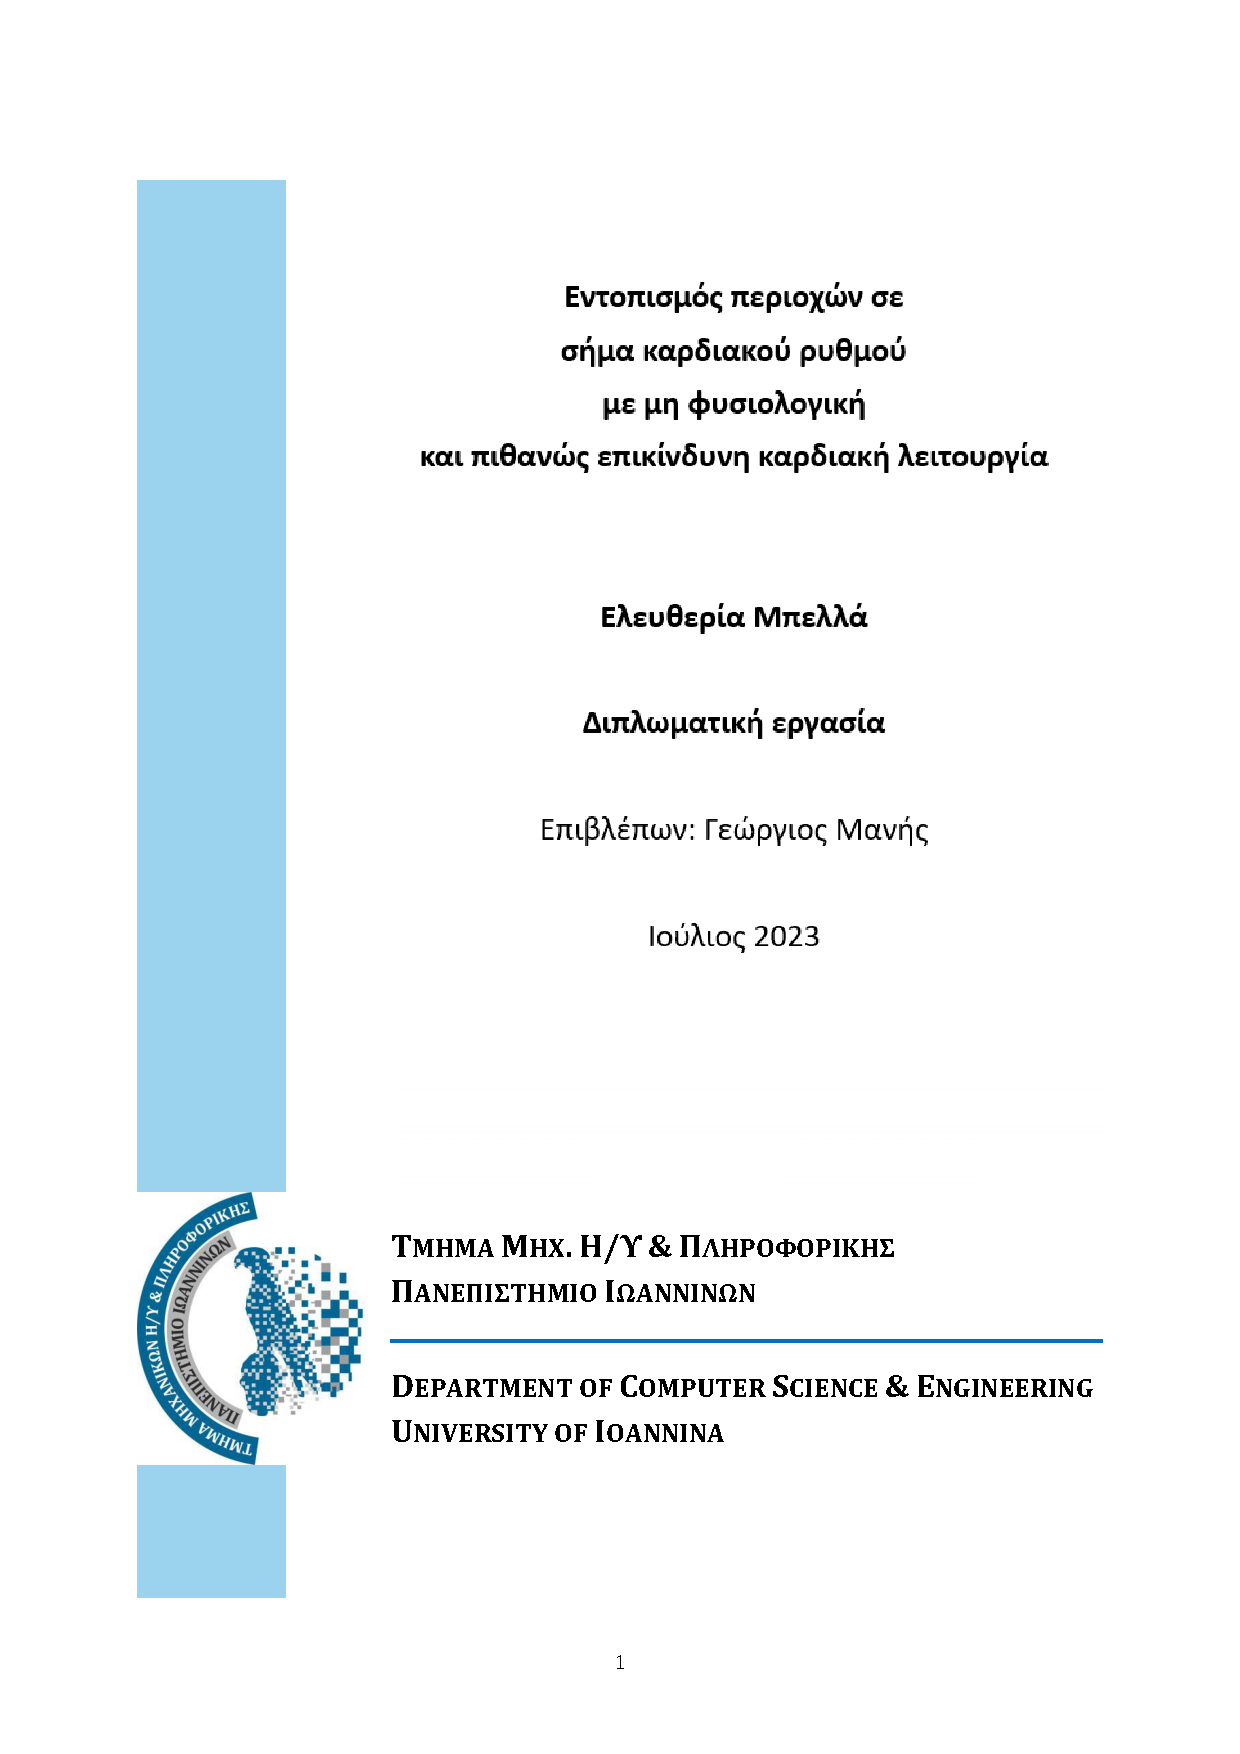
\includegraphics[width=\paperwidth, height=\paperheight]{intro.pdf}
	}
}
\newpage


\begin{document}
\chapter*{}
\chapter*{Ευχαριστίες}
Θα ήθελα να ευχαριστήσω τον επιβλέποντά μου, Γεώργιο Μανή, για την εμπιστοσύνη και την υπομονή που έδειξε κατά τη διάρκεια εκπόνησης αυτής της εργασίας.
\chapter*{Αφιέρωση}
\gr Στη μαμά μου.

\gr
\chapter*{Εκτεταμένη Περίληψη}
Η ανθρώπινη καρδιά, αν και έχει μέγεθος ανθρώπινης γροθιάς, καταφέρνει να αντλεί αίμα σε ολόκληρο το σώμα χωρίς κανένα διάλειμμα. Μέσω των συσπάσεών της, η καρδιά ωθεί το αίμα προς τα διαφορετικά όργανα, ενώ το "αφιλτράριστο" αίμα επιστρέφει σε αυτήν ώστε να καθαριστεί και να επαναλάβει τον κύκλο του. Ένας τέτοιος κύκλος αποτελεί τον καρδιακό παλμό, με το σύνολο των τελευταίων να ορίζουν τον καρδιακό ρυθμό. Οι καρδιακές συσπάσεις γίνονται δυνατές μέσω ηλεκτρικών ώσεων χαμηλής έντασης οι οποίες εξαναγκάζουν τον μυ της καρδιάς σε κίνηση.
\par
Η μεταβολή των καρδιακών παλμών απεικονίζεται στο ηλεκτροκαρδιογράφημα, μια ιατρική εξέταση που συμβάλλει στην πρόληψη καρδιακών παθήσεων και στην αξιολόγηση της υγείας του μυοκαρδίου. Η διακύμανση των παλμών ονομάζεται μεταβλητότητα του καρδιακού παλμού και αποτελεί σημαντικό δείκτη για τη φυσική κατάσταση της καρδιάς. Μετράται με πολλές διαφορετικές μεθόδους, αρκετές εκ των οποίων στοχεύουν στην εκτίμηση της πολυπλοκότητας του καρδιακού παλμού, αποτελώντας, έτσι, ένα σημαντικό εργαλείο στην αξιολόγηση της καρδιακής λειτουργίας. Είναι ωστόσο σημαντικό να αναφερθεί πως η καταγραφή που πραγματοποιείται μέσω του ηλεκτροκαρδιογραφήματος είναι συχνά ατελής, καθώς εξωγενείς και ενδογενείς παράγοντες εισάγουν θόρυβο και αλλοιώνουν το τελικό αποπτέλεσμα.
\par
Στις περιπτώσεις στις οποίες η άντληση του αίματος παρουσιάζει αποκλίσεις, παρουσιάζεται απώλεια φυσιολογικού παλμού και ελαττωματική λειτουργία της καρδιάς. Οι δυσλειτουργίες αυτές ονομάζονται αρρυθμίες και όταν εμφανίζονται μεμονωμένα δεν αποτελούν κίνδυνο. Ωστόσο, η επανειλημμένη εμφάνισή τους χρίζει εξέτασης, προκειμένου να προληφθούν και να αποφευχθούν σοβαρές επιπλοκές. Οι καρδιακές αρρυθμίες ανάλογα με το τμήμα της καρδιάς από το οποίο ξεκινούν χωρίζονται σε δύο γενικές κατηγορίες: τις κολπικές, όταν ξεκινούν από τους κόλπους της καρδιάς και τις κοιλιακές, όταν ξεκινούν από τις κοιλίες. Επιπλέον, οι αρρυθμίες χωρίζονται σε ταχυκαρδίες, οι οποίες χαρακτηρίζονται από αύξηση του καρδιακού ρυθμού και βραδυκαρδίες, οι οποίες συνδέονται με μείωσή του.
\par
Λόγω της σύνθετης φύσης των αρρυθμιών και των διαφόρων παραγόντων που επηρεάζουν τη μορφολογία τους, κρίνεται επιτακτική η ανάπτυξη εργαλείων για αξιολόγηση και πρόληψη τους. Για την επίτευξη του παραπάνω στόχου, έχουν αναπτυχθεί εξετάσεις και αλγόριθμοι που «φιλτράρουν» το καρδιακό σήμα, απομακρύνοντας πηγές θορύβου που μπορεί να το αλλοιώνουν, εφαρμόζουν μετρικές και μεθόδους ανθεκτικές σε αυτόν και καταφέρνουν να εντοπίσουν σημεία αποκλίνουσας καρδιακής δραστηριότητας. 
\par
Η ακόλουθη εργασία έχει ως στόχο την σύνθεση ενός αλγορίθμου, ο οποίος βασίζεται στη χρήση ευρέως αποδεκτών μεθόδων εκτίμησης εντροπίας και πολυπλοκότητας του σήματος. Η χρήση πραγματικών καρδιακών σημάτων, από άτομα διαφορετικών ηλικιών, φύλων, με διαφορετικές καρδιακές παθήσεις που μελετώνται δίνει μια πιο ολοκληρωμένη άποψη για την απόδοση του αλγορίθμου, ο οποίος μελετά την πρόβλεψη κάθε μετρικής και μεθόδου σε μικρά χρονικά μεταβαλλόμενα «παράθυρα», τμήματα δηλαδή του σήματος. Η ανάπτυξη του αλγορίθμου αυτού αποσκοπεί στον εντοπισμό αρρυθμιών με όσο το δυνατόν υψηλότερη ακρίβεια, καθώς η βάση του αποτελείται από πραγματικές καταγραφές καρδιακών σημάτων διαφορετικών καρδιακών παθήσεων και αποτελεί τον πυρήνα μελέτης αυτής της διπλωματικής εργασίας.

\en
\en
\chapter*{Abstract}
The human heart, although it is the size of a human fist, manages to pump blood to the entire human body, continuously. Thanks to its contractions, it pushes the blood to the different organs while the 'unfiltered' blood returns to it so it can be cleaned and repeat the same cycle. This cycle is what we call a heart beat, the total of  which define the heart rhythm.  These contractions are possible because of low current signals that force the heart muscle to move.
\par
The alteration of heart beats can be depicted in a electrocardiogram, a medical test that aids the prevention of heart conditions and evaluation of the heart's physical state. The variability between these pulses is called heart rate variability and it defines an important index related to the heart's physical condition. What is worth mentioning that the recording performed during the electrocardiogram is often faulty, due to noise introduced to the signal because of outer and inner factors. 
\par
In cases that the pumping of blood deviates from normal, there is loss of normal heart beats and the function of the heart becomes defective. These events are called arrhythmias, and they pose no threat if not repeated. When they do, though, the patients needs to undergo tests in order to be prevented. Hearth arrhythmias are categorized in atrial, when they are generated in the atrias of the heart and ventricular when they occur in the ventricles. Moreover, they are also dividen into tachyarrhythmias, which are related to a higher heart rhythm and bradyarrhythmias, which are characterized by a slower heart rhtyhm.
\par
Due to the complex nature of arrhythmias and the factors that are involved in their morphology, it is imperative that tools for their evaluation and prevention are developed. For this goal to be accomplished, there are medical tests and algorithms that have been factored so they can filter out the noise from the heart signal that might alter it. They are also capable of applying metrics and methods to it so they can locate areas of abnormal heart activity.
\par
The following thesis aims to an algorithm development that is based on the use of widely accepted entropy and signal complexity estimation methods. Also, the studying of actual heart signals taken from actual people of different age, sex who might suffer from various heart conditions, gives a more comprehensive view of the algorithm's performance; the algorithm studies the each metric and method in small time-varying 'windows', which are signal portions. This algorithm aims to identify arrhythmias as accurately as possible, as its basis consists of real heart signal recordings of different heart diseases, which is the core of this study.
\gr

\thispagestyle{empty}
\tableofcontents
\listoffigures
\listoftables
\newpage

\chapter{Η ανθρώπινη καρδιά}
\gr
Σε αυτό το κεφάλαιο θα πραγματοποιηθεί αναλυτική περιγραφή της ανθρώπινης καρδιάς. Θα παρουσιαστεί η ανατομία, η λειτουργία της, θα αναλυθεί ο καρδιακός κύκλος και θα παρουσιαστεί η έννοια της καρδιακής μεταβλητότητας (\en Heart Rate Variability, HRV). \gr Τέλος, θα παρουσιαστούν οι καταστάσεις κατά τις οποίες η ανθρώπινη καρδιά δε λειτουργεί ομαλά και φυσιολογικά, ονομαζόμενες και αρρυθμίες  και θα αναλυθούν οι διαφορετικές κατηγορίες ανάλογα με το διαμέρισμα από το οποίο προέρχονται και το αποτέλεσμα που έχουν στον καρδιακό παλμό.
\begin{figure}[h]
     \centering
     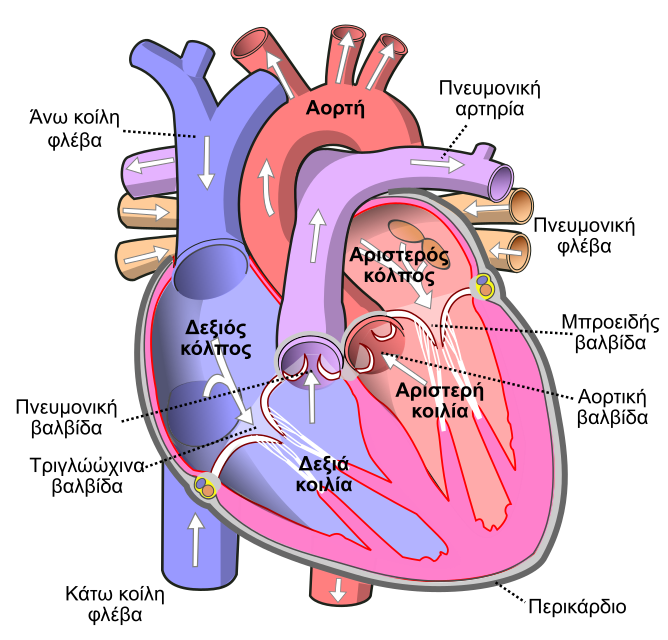
\includegraphics[scale=0.25]{human heart.png}
     \caption{Η ανθρώπινη καρδιά, \en\protect\url{https://en.wikipedia.org/}}
 \end{figure}
\section{Ανατομία και λειτουργικότητα}
Η λειτουργία του ανθρώπινου οργανισμού βασίζεται στην καρδιά, ένα μυ ελαφρώς μεγαλύτερο από μία γροθιά. Αν και τόσο μικρή, καταφέρνει να αντλεί με ευκολία το αίμα σε όλο το σώμα και ταυτόχρονα να φιλτράρει όσο αίμα φτάνει σε εκείνη, εκτελώντας το ρόλο της με απόλυτη επιτυχία. Βρίσκεται κάτω από το θώρακα, συνήθως στην αριστερή πλευρά (σε σπάνιες περιπτώσεις, μπορεί να βρεθεί και στα δεξιά). Αποτελείται από τέσσερα βασικά διαμερίσματα: στο άνω μέρος βρίσκονται οι κόλποι, οι οποίοι λαμβάνουν το αίμα που φτάνει στην καρδιά από το ανθρώπινο σώμα. Στο κάτω μέρος, οι κοιλίες, δέχονται το αίμα από τους κόλπους και το προωθούν εκτός της καρδιάς, αποβάλλοντας το αίμα προς το σώμα. Αν και αυτά τα τέσσερα τμήματα φαίνονται ενιαία, χωρίζονται μεταξύ τους με διαφορετικές μεμβράνες. Το αριστερό και το δεξί τμήμα του καρδιακού μυ διαχωρίζονται από το διάφραγμα, μια μυϊκή δομή που εμποδίζει την ανάμειξη του αίματος ανάμεσα στα δύο τμήματα. Παράλληλα, οι καρδιακές βαλβίδες διαχωρίζουν τους κόλπους από τις κοιλίες. Συμβάλλουν στην αποφυγή της παλινδρόμησης και τη σωστή ροή του αίματος ανάμεσα στα καρδιακά διαμερίσματα. Οι βαλβίδες υπόκεινται σε διαφορετικές πιέσεις στις δύο τους πλευρές και ανοίγουν μονόδρομα προς την επιθυμητή κατεύθυνση. [1]-[3]

\section{Καρδιακός κύκλος}
Ο καρδιακός κύκλος αποτελείται από δύο ξεχωριστές καταστάσεις: τη συστολή και τη διαστολή. Η εναλλαγή τους αποτελεί έναν αέναο κύκλο, εξ ου και το όνομα. Κατά τη διαστολή, το αίμα αντλείται μέσα στην καρδιά από τς φλέβες (εκτός από την πνευμονική \en pulmonary \gr), οι οποίες μεταφέρουν το ανοξυγωνομένο αίμα από τα διαφορετικά σημεία του σώματος μεταφέρεται στους πνεύμονες ώστε να οξυγονωθεί. 
Αντίθετα, κατά τη συστολή, το αίμα, που είναι πλέον οξυγονωμένο, μεταφέρεται μέσω των αρτηριών (εκτός της πνευμονικής \en pulmonary \gr) πίσω στα διαφορετικά σημεία του σώματος. Οι φλέβες και οι αρτηρίες αποτελούν τα αιμοφόρα αγγεία του ανθρώπινου σώματος. Η διαδικασία αυτή έχει ως αποτέλεσμα την παραγωγή ηλεκτρικών ώσεων. Η έναρξη αυτής της διαδικασίας αποτελεί την αρχή του καρδιακού χτύπου και το πέρας της το τέλος του, αντίστοιχα. 
\subsection{Γεγονότα  του καρδιακού κύκλου}
Πιο αναλυτικά, τα γεγονότα του καρδιακού κύκλου είναι τα εξής:
\begin{itemize}
    \item Στο δεξιό κόλπο, οι φλέβες μεταφέρουν το μη οξυγωνομένο αίμα που έχει συλλεχθεί. 
    \item Το αίμα μεταφέρεται από το δεξιό κόλπο στη δεξιά κοιλία.
    \item Το αίμα στέλνεται στους πνεύμονες μέσω τις πνευμονικής αρτηρίας.
    \item Οι πνευμονικές φλέβες στέλνουν το αίμα στον αριστερό κόλπο, απομακρύνοντάς το από τους πνεύμονες.
    \item Το αίμα στέλνεται πίσω σε όλους τους ιστούς, έχοντας μεταφερθεί στην αριστερή κοιλία, μέσω της αορτής. [1]-[6]
\end{itemize}
\subsection{Καρδιακός ρυθμός}
Μία τέτοια εναλλαγή συστολής-χαλάρωσης αποτελεί, όπως ειπώθηκε τον καρδιακό παλμό. Ο παλμός αποτελεί τη βάση για τη μονάδα μέτρησης της κατάστασης της καρδιάς, που μετράται με τον καρδιακό ρυθμό, δηλαδή το πλήθος των παλμών ανά λεπτό (\en beats per minute, BPM \gr). Τα κύτταρα στα οποία καθιστάται εφικτή η παραπάνω εναλλαγή είναι δύο τύπων καρδιακά μυϊκά κύτταρα: τα συσταλτά και τα αυτορρυθμικά. Τα συσταλτά κύτταρα ευθύνονται για τα μηχανικά γεγονότα του κύκλου που οδηγούν στην εξώθηση του αίματος. Τα κατάλληλα ηλεκτρικά ερεθίσματα για τη συστολή τους προέρχονται από τα αυτορρυθμικά κύτταρα, τα οποία είναι ενδογενώς ικανά να πυροδοτούν δυναμικά. [1]-[6]

\begin{figure}
    \centering
    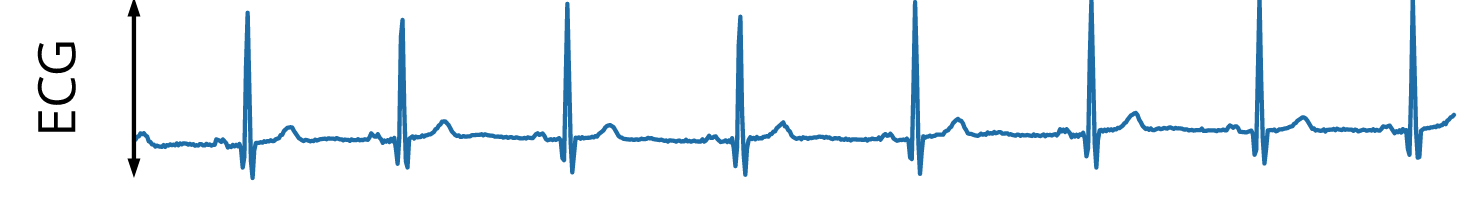
\includegraphics[scale=0.3]{heart rhythm.png}    \caption{Απεικόνιση καρδιακού ρυθμού κατα την καταγραφή ΗΚΓ \en \protect\url{https://en.wikipedia.org/}}
\end{figure}

\section{Τμήματα καρδιακού παλμού και Ηλεκτροκαρδιογράφημα}
Όπως αναφέρθηκε, η καρδιά αποτελεί ένα σύνθετο όργανο του ανθρώπινου σώματος και μέσα από την διαδοχή των διαστολών και συστολών καταφέρνει να χτυπάει ρυθμικά, παράγοντας ηλεκτρικές ώσεις. Οι ώσεις αυτές προέρχονται από το φλεβόκομβο, που βρίσκεται στο τοίχωμα του δεξιού κόλπου. Ηλεκτρικά σήματα που παράγονται από τα αυτορρυθμικά κύτταρα του φλεβόκομβου, φτάνουν στους κόλπους, αναγκάζοντάς τους να συσπαστούν (Ρ κύμα, ή έπαρμα). Στη συνέχεια το σήμα αυτό περνά από τον κολποκοιλιακό κόμβο, που εντοπίζεται πάνω από την ένωση των κόλπων με τις κοιλίες (\en atrioventricular node, AV\gr) και μειώνει το σήμα προτού επιτραπεί να περάσει στις κοιλίες. Η καθυστέρηση αυτή εξυπηρετεί στο να αδειάσουν πλήρως οι κόλποι από αίμα, προτού αυτό μεταφερθεί στις κοιλίες. Έπειτα, το σήμα περνά από τις ίνες \en Purkinje \gr και κάνει τις κοιλίες να συσπαστούν (σύμπλεγμα \en QRS\gr ). Η επαναφορά στο δυναμικό ηρεμίας (επαναπόλωση) των κοιλιών αποτελεί το έπαρμα Τ.
\par 
Ο κάθε χτύπος αποτελείται από μια εναλλαγή καταστάσεων στα διαφορετικά διαμερίσματα της καρδιάς (τους κόλπους και τις κοιλίες) και πιο συγκεκριμένα την εκπόλωση και την επαναπόλωσή τους. Τα βασικά αυτά τμήματα είναι τα ακόλουθα:

\begin{itemize}
    \item το Ρ κύμα ή έπαρμα, που αντιστοιχεί στην ηλετρική διέγερση (εκπόλωση) των κόλπων,
    \item το σύμπλεγμα \en QRS, \gr που αντιστοιχεί στην κοιλιακή διέγερση, 
    \item το Τ κύμα ή έπαρμα, που σε συνδυασμό με το \en U \gr έπαρμα (κύμα) αποτελεί την κοιλιακή επαναπόλωση (επιστροφή σε κατάσταση ηρεμίας).
\end{itemize}
 Οι εναλλαγές ανάμεσα σε αυτά τα τμήματα δημιουργούν μια συγκεκριμένη 
 επαναλαμβανόμενη κυματομορφή, η οποία αποτελεί έναν καρδιακό παλμό. Αποτελεί το μέτρο σύγκρισης για την ερμηνεία της φυσιολογικής (και μη) καρδιακής λειτουργίας και προσφέρει διαγνωστικές πληροφορίες. 
 \par
 Αυτές οι διαδοχικές αλλαγές αποτυπώνονται στο ηλεκτροκαρδιογράφημα (ΗΚΓ), ένα ισχυρό διαγνωστικό εργαλείο για ποικίλες παθήσεις της καρδιάς. Μέσω της τοποθέτησης ηλεκτροδίων σε διαφορετικά σημεία του σώματος του ασθενούς, ο καρδιακός ρυθμός αποτυπώνεται με μεγάλη ακρίβεια και επιτρέπει είτε την επιβεβαίωση μιας φυσιολογικής λειτουργίας, είτε τη διάγνωση ή και πρόληψη καρδιακών παθήσεων και ανωμαλιών. Μέσω του ΗΚΓ μπορούν να αξιολογηθούν πολλές πλευρές της καριδακής λειτουργίας, όπως η αγωγιμότητά της, ακόμα και διαταραχές όπως ισχαιμία και αρρυθμίες. Οι καρδιακές ηλεκτρικές ώσεις αποτυπώνονται στο ΗΚΓ, διευκολύνοντας την ερμηνεία τους. Ως παραδείγματα δίνονται τα εξής:
 \begin{itemize}
     \item επιμήκυνση του συμπλέγματος \en QRS \gr αποτυπώνει υψηλό κίνδυνο για κοιλιακές αρρυθμίες (μη φυσιολογική λειτουργία, δηλαδή, των κοιλιών)
     \item αλλοίωση του τμήματος \en ST\gr (το διάστημα ανάμεσα στα σημεία \en S \gr και Τ μπορεί να προμηνύουν έμφραγμα).
 \end{itemize}
 Το ΗΚΓ χρησιμοποιείται επίσης για παρακολούθηση κατά τη διάρκεια καρδιακών επεμβάσεων. Αποτελεί ένα μη επεμβατικό και χρησιμοποιούμενο ευρέως εργαλείο στην ιατρική και όχι μόνο κοινότητα. [6]-[8]

\subsection{Επιπλέον παράμετροι του καρδιακού κύκλου}
\begin{itemize}
    \item Διάστημα \en RR\gr : Το διάστημα που μεσολαβεί ανάμεσα σε δύο διαδοχικές R κορυφές. Χρησιμοποιείται για τη μέτρηση του καρδιακού παλμού.
    \item Διάστημα \en PR\gr : Το χρονικό διάστημα που χρειάζεται για να φτάσει το ηλεκτρικό ρεύμα στις κοιλίες(χρονική διάρκεια: 120-200\en msec).\gr
    \item Τμήμα \en PR\gr: Συνδέει το έπαρμα Ρ με το \en QRS \gr σύμπλεγμα. Η καθυστέρηση μετάδοσης της ώσης από τον κόλπο στην κοιλία. Για αυτό το λόγο εμφανίζεται στο ΗΚΓ ως μια ευθεία γραμμή (χρονική διάρκεια: 50-120 \en msec).\gr
    \item Τμήμα \en ST\gr : Η περίοδος κατά την οποία οι κοιλίες παραμένουν εκπολωμένες. Συνδέει το \en QRS \gr σύμπλεγμα με το έπαρμα Τ (χρονική διάρκεια: 80-120 \en msec).\gr
    \item Σημείο \en J\gr : Το σημείο στο οποίο το \en QRS \gr σύμπλεγμα τελειώνει και αρχίζει το τμήμα \en ST.\gr
    \item Διάστημα \en ST\gr : Μετράται από το σημείο \en J \gr  έως το τέλος του επάρματος Τ (χρονική διάρκεια: 320 \en msec).\gr
    \item Διάστημα \en QT\gr : Μετράται από την αρχή του \en QRS \gr διαστήματος έως και το τέλος του επάρματος Τ. Μεγαλύτερο διάστημα από το αναμενόμενο μπορεί να προμηνύει ταχυκαρδία ή και θάνατο (χρονική διάρκεια έως και 420 \en msec \gr με καρδιακό ρυθμό 60 χτύπων ανά λεπτό). [6]-[8]
\end{itemize}

\begin{figure}[h]
    \centering
    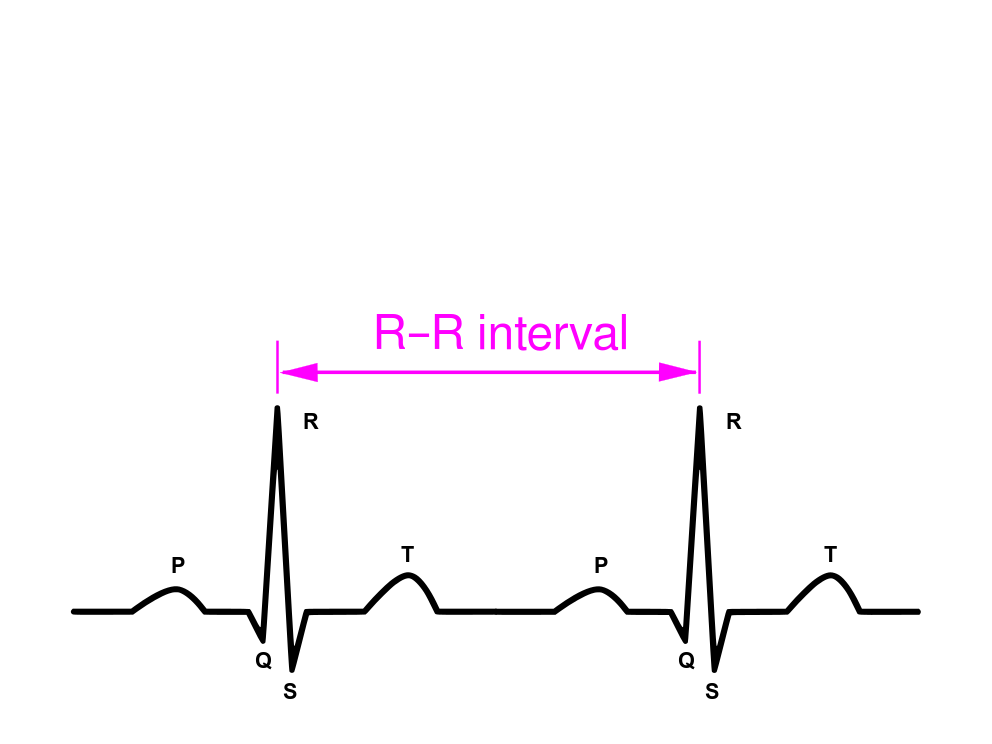
\includegraphics[scale=0.25]{RRinterval.png}
    \caption{Διάστημα \en RR: \gr Βασική μονάδα μέτρησης του καρδιακού ρυθμού \en \protect\url{https://en.wikipedia.org/}}
\end{figure}

\section{ΗΚΓ: Απόκλιση από τη φυσιολογική καταγραφή - Θόρυβος}
Παρόλη την εγκυρότητα του ΗΚΓ κατά την καταγραφή της ηλεκτρικής δραστηριότητας της καρδιάς, το αποτέλεσμα μπορεί συχνά να μην είναι τέλειο. Συχνό φαινόμενο είναι η παρεμβολή διάφορων σημάτων που εμποδίζουν την πραγματική απεικόνιση της καρδιακής λειτουργίας. Τέτοιου είδους σήματα ονομάζονται θόρυβος και μπορεί να προέρχονται από: τη μη σταθερή επαφή των ηλεκτροδίων με το δέρμα του ασθενούς, από διαταραχές στη γραμμή τροφοδοσίας, την κίνηση του ασθενούς κατά τη διάρκεια της καταγραφής ή διάταση του δέρματος (μοιάζει με διαταραχή στη γραμμή βάσης, είναι όμως δυσκολότερα αντιμετωπίσιμη). 
\par
Αυτές οι αποκλίσεις δημιουργούν θόρυβο στο σήμα, επηρεάζουν τη μορφολογία των διάφορων τμημάτων του καρδιακού παλμού και οδηγούν στη λανθασμένη καταγραφή ολόκληρων παλμών. Ένα μέρος του θορύβου μπορεί να αφαιρεθεί με σύγχρονες τεχνικές αλλά η καταγραφή θα παραμένει σε ένα ποσοστό ατελής. [8]-[10] 
\subsection{Καρδιακές ασθένειες που ανιχνεύονται μέσω του ΗΚΓ}
\begin{itemize}
    \item Ταχυκαρδία: Κατάσταση κατά την οποία οι καρδιακοί παλμοί είναι αφύσικα αυξημένοι (πάνω από 100 το λεπτό)
    \item Βραδυκαρδία: Κατάσταση κατά την οποία οι καρδιακοί παλμοί είναι αφύσικα μειωμένοι (λιγότεροι από 60 το λεπτό)
    \item Σύνδρομο εκτενούς \en QRS \gr συμπλέγματος: Καρδιακή πάθηση κατά την οποία υπάρχει καθυστέρηση μεγαλύτερη του φυσιολογικού μεταξύ της εκπόλωσης και επαναπόλωσης των κοιλιών.
    \item Σύνδρομο βραχέος \en QRS \gr συμπλέγματος: Γενετική πάθηση που οφείλεται σε πολύ σύντομα διαστήματα \en QT \gr διαστημάτων στο ΗΚΓ. \en
    \item Heart block \gr πρώτου βαθμού: Πάθηση σχετική με την αγωγιμότητα της καρδιάς.\en 
    \item Heart block \gr δεύτερου βαθμού: Σποραδική απουσία \en QRS \gr συμπλέγματος και Τ επάρματος μετά από έπαρμα Ρ που προέρχεται από τους καρδιακούς κόλπους. [7]-[9]
\end{itemize}
\begin{figure}[h]
    \centering
    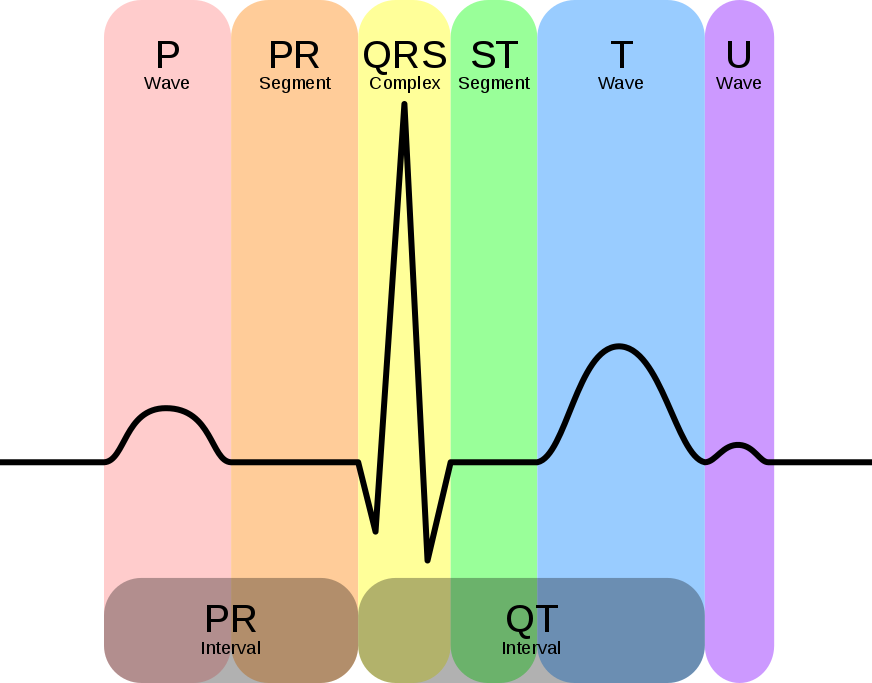
\includegraphics[scale=0.2]{heart beat.png}
    \caption{Αναπαράσταση καρδιακού παλμού, \en\protect\url{https://en.wikipedia.org/}}
\end{figure}

\section{Διακύμανση καρδιακού ρυθμού - \en Heart Rate Variability (HRV)}\gr
Η διαφορά των χρονικών διαστημάτων ανάμεσα σε διαφορετικούς καρδιακούς παλμούς ονομάζεται διακύμανση καρδιακού ρυθμού. Η διακύμανση αυτή υποδηλώνει το πόσο εύκολα (ή δύσκολα) μπορεί η καρδιά να προσαρμόζεται σε διαφορετικές σωματικές καταστάσεις καθώς και τη δυνατότητά της να επαναφέρει τον καρδιακό ρυθμό σε φυσιολογικά επίπεδα σε κατάσταση ηρεμίας. Αυτό απεικονίζεται ως εξής: μια υγιής καρδιά έχει υψηλό \en HRV \gr διότι προσαρμόζει εύκολα τον καρδιακό ρυθμό (από αδράνεια σε σωματική άσκηση, από κατάσταση ηρεμίας σε κατάσταση φόβου/πανικού και αντίστροφα) ενώ μια ασθενής καρδιά έχει χαμηλό \en HRV, \gr (πάντα συγκριτικά με τη μέση καρδιακή λειτουργία του κάθε ανθρώπου ή κάποιο σταθερό εύρος τιμών, σύμφωνα με κάποια γενική αποδεκτή μέση τιμή) μιας και αδυνατεί να προσαρμοστεί ή χρειάζεται περισσότερο χρόνο από το φυσιολογικό. Οι παράγοντες που επηρεάζουν τη διακύμανση καρδιακού ρυθμού μπορούν να είναι τόσο ενδογενείς όσο και εξωγενείς. Πιο συγκεκριμένα:
\begin{itemize} 
    \item Το φύλο. Η γυναικεία καρδιά έχει χαμηλότερο \en HRV \gr από την ανδρική (οι παλμοί είναι μικρότεροι, άρα τα τμήματα είναι επίσης μικρότερα).
    \item Η ηλικία. Όσο νεότερος είναι ένας άνθρωπος, τόσο πιο εύκολα ακολουθεί τις αλλαγές στη σωματική του κατάσταση. Επομένως τόσο πιο ψηλό είναι και το \en HRV \gr του.
    \item Ασθένειες. Αυτές μπορούν να είναι τόσο επίκτητες όσο και εκ γενετής. Ενδεικτικά, μία από αυτές τις ασθένειες είναι το έμφραγμα του μυοκαρδίου (ασθενείς που έχουν περάσει έμφραγμα συχνά παρουσιάζουν χαμηλότερο \en HRV\gr).
    \item Εξωγενείς παράγοντες. Μερικοί από αυτούς είναι το άγχος, το κάπνισμα, καταστάσεις συναισθηματικής φόρτισης (όπως υπερένταση), αντιαρρυθμικά φάρμακα αλλά και πολλούς άλλους.
\end{itemize} 
\par
Μια υγιής καρδιά δεν εμφανίζει μετρονομικά την απόλυτη ομοιομορφία ανάμεσα στους διαδοχικούς παλμούς και χαρακτηρίζεται από υψηλή μεταβλητότητα, όμοια με μαθηματικό μοντέλο. Παρόλη την ανομοιομορφία, οι καρδιακές παθήσεις και ασθένειες χαρακτηρίζονται από υπέρμετρη αύξηση ή απώλεια πολυπλοκότητας σε σύγκριση με αυτή του φυσιολογικού. Συνήθως οι καρδιακές παθήσεις που αυξάνουν το \en HRV \gr συνδέονται με αυξημένη πιθανότητα θνησιμότητας. Επομένως, η βασική διαφορά ανάμεσα στις αριθμητικές τιμές της καρδιακής μεταβλητότητας είναι η δυνατότητα επαναφοράς της στα φυσιολογικά επίπεδα χωρίς εξωτερική παρέμβαση. [11]-[12]

\section{Ρύθμιση \en HRV \gr – Αυτόνομο Νευρικό Σύστημα}
\begin{figure}[h]
    \centering
    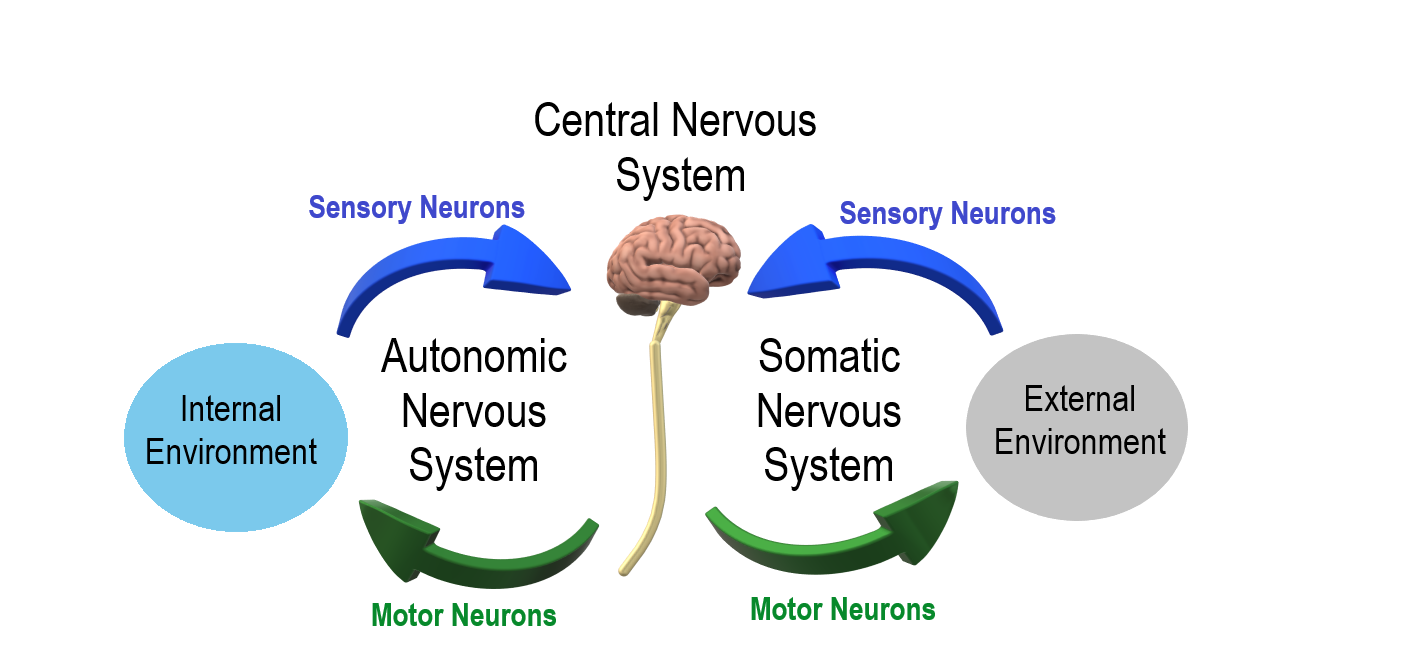
\includegraphics[scale=0.3]{Autonomic_and_Somatic_Nervous_System.png}
    \caption{Το κεντρικό νευρικό σύστημα \en \protect\url{https://en.wikipedia.org/}}
\end{figure}
Το \en HRV \gr ρυθμίζεται από τη συνδυαστική δράση του Αυτόνομου Νευρικού Συστήματος (ΑΝΣ) και του
φλεβόκομβου. Το ΑΝΣ επηρεάζει τη λειτουργία των περισσότερων ιστών και οργάνων του ανθρώπινου οργανισμού, ασκώντας τη δράση του στους λείους μύες, την καρδιά, τους ενδοκρινείς και εξωκρινείς
αδένες. Συγκεκριμένα, ρυθμίζει τον καρδιακό χτύπο, τη θερμοκρασία του σώματος, την εφίδρωση,
την πίεση του αίματος κ.ά., συμβάλλοντας, έτσι, στη διατήρηση της ομοιόστασης. Διχοτομείται σε
δύο κλάδους, μορφολογικά και λειτουργικά ανεξάρτητους: το συμπαθητικό και το παρασυμπαθητικό
σύστημα. Το συμπαθητικό σύστημα προετοιμάζει τον οργανισμό για την αντιμετώπιση στρεσογόνων
καταστάσεων, αυξάνοντας τον καρδιακό ρυθμό και διεγείροντας την παραγωγή ενέργειας. Αντίθετα, το παρασυμπαθητικό σύστημα ρυθμίζει τις σωματικές διεργασίες σε καταστάσεις ηρεμίας και μειώνει τον καρδιακό ρυθμό. Συνεπώς, τα δύο αυτά συστήματα δρουν προς διαφορετικές κατευθύνσεις, δημιουργώντας διαφορές στον καρδιακό παλμό, αυξάνοντας έτσι το  \en HRV. [11]-[17] \gr 
\par
Στα επόμενα κεφάλαια θα παρουσιαστεί πιο αναλυτικά η ρύθμιση του \en HRV \gr και οι ποικίλοι τρόποι μέτρησής του, το πώς επηρεάζεται όταν ο καρδιακός ρυθμός αποκλίνει από το φυσιολογικό και με ποιους τρόπους αυτός αποκλίνει.
\par
\newpage
\gr
\chapter{Καρδιακές αρρυθμίες}
Στο προηγούμενο κεφάλαιο παρουσιάστηκε η ανατομία και η βασική λειτουργία της ανθρώπινης καρδιάς, ο καρδιακός ρυθμός (Σχήμα 2.1), η απεικόνισή του και η ερμηνεία του μέσω του ΗΚΓ (Σχήμα 2.2). Μέσω αυτού του εργαλείου είναι εφικτή η διάγνωση και η πρόληψη ποικίλων καρδιακών δυσλειτουργιών. Όταν οι δυσλειτουργίες αυτές δεν οφείλονται σε θόρυβο από το εξωτερικό περιβάλλον και το ΗΚΓ, προέρχονται από έναν καρδιακό ρυθμό που αποκλίνει του φυσιολογικού. Οι καταστάσεις αυτές ονομάζονται αρρυθμίες και θα αναλυθούν στο τρέχον κεφάλαιο. Πιο συγκεκριμένα, θα παρουσιαστεί ο ακριβής ορισμός της αρρυθμίας, ποια διαμερίσματα της καρδιάς αντιστοιχούν σε ποιες κατηγορίες αρρυθμιών, πώς αποτυπώνονται στο καρδιογράφημα, αλλά και με ποιες μεθόδους υπολογίζονται. \par
%\section{Ορισμός}
Ο όρος αρρυθμία καλύπτει ένα ευρύ φάσμα καρδιακών φαινομένων και αναταραχών. Ως καρδιακή αρρυθμία ορίζεται η απόκλιση από το φυσιολογικό παλμό. Κατά τη διάρκεια των αρρυθμιών ο παλμός της καρδιάς μπορεί να είναι πολύ χαμηλός, πολύ υψηλός ή εντελώς ακανόνιστος. 
\par
Όπως σχολιάστηκε στο προηγούμενο κεφάλαιο, ένας φυσιολογικός παλμός παράγεται από το φλεβόκομβο (\en SA node \gr) και στη συνέχεια επιβραδύνεται καθώς περνά από τον κολποκοιλιακό κόμβο (\en AV node\gr ). Έπειτα, περνά στα τέσσερα κύρια διαμερίσματα της καρδιάς, τους κόλπους και τις κοιλίες και τέλος σε όλα τα διαφορετικά σημεία του σώματος. Οποιαδήποτε κατάσταση αποκλίνει από αυτή θεωρείται αρρυθμία.
\par
Οι αρρυθμίες χωρίζονται σε δύο μεγάλες κατηγορίες: τις βραδυκαρδίες, δηλαδή καταστάσεις στις οποίες ο καρδιακός παλμός είναι χαμηλότερος του κανονικού μέσου όρου (60 παλμοί το λεπτό) και τις ταχυκαρδίες, καταστάσεις στις οποίες ο καρδιακός παλμός αυξάνεται σε σημείο άνω του φυσιολογικού ανθρώπινου (100 παλμοί το λεπτό). Ειδικότερα, οι αρρυθμίες χωρίζονται με βάση το σημείο προέλευσης, τον τρόπο μετάδοσης και τις ασθένειες με τις οποίες συσχετίζονται. Οι αρρυθμίες μπορεί να εμφανίζονται μεμονωμένα (ένας μεμονωμένος αποκλίνων χτύπος) αλλά και σε σύνολα (δύο, τρεις ή και περισσότεροι συνεχόμενοι μη φυσιολογικοί παλμοί που αποτυπώνονται στο ΗΚΓ σε μοτίβα). 
\par
Τα άτομα που εμφανίζουν καρδιακές αρρυθμίες ενδέχεται να πάσχουν από κάποια ασθένεια ή και να είναι απόλυτα υγιή, καθώς οι αρρυθμίες σε μικρό ποσοστό, είναι απολύτως φυσιολογικές. Σε περιπτώσεις όμως, που εμφανίζονται τακτικά μπορεί να υποδείξουν κάποιο υποκείμενο νόσημα επικίνδυνο για την υγεία. Η γενική παρουσία αρρυθμιών συσχετίζεται με υψηλότερη πιθανότητα νοσηρότητας και θνησιμότητας [18]-[22], [24], [26]-[28]. 
\begin{figure}[b]
	\centering
	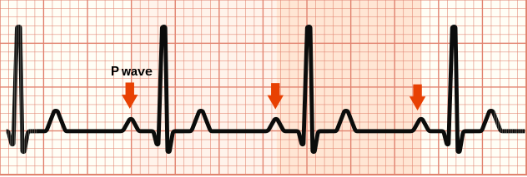
\includegraphics[scale=0.5]{normal.png}
	\caption{Φυσιολογικός καρδιακός ρυθμός \en\protect\url{https://commons.wikimedia.org/wiki/Main_Page}}
\end{figure}
\section{Κατηγοριοποίηση αρρυθμιών}
Οι αρρυθμίες μπορούν να χωριστούν στις ακόλουθες γενικές κατηγορίες:
\begin{figure}[h]
	\centering
	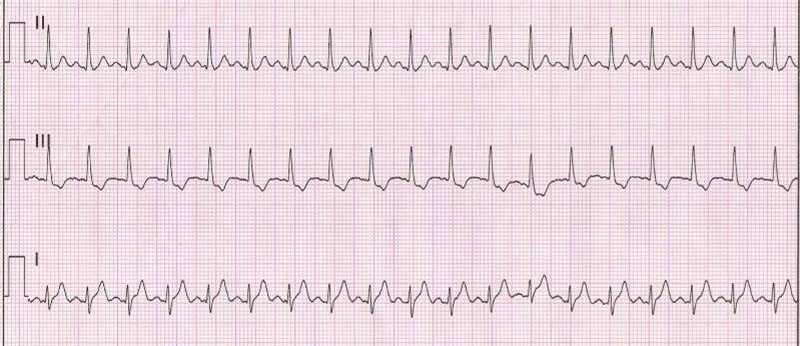
\includegraphics[scale=0.3]{Sinus_Tachycardia_Unlabeled.jpg}
	\caption{Τυπική αναπαράσταση ταχυκαρδίας σε ΗΚΓ \en\protect\url{https://en.wikipedia.org/}}
\end{figure}
\subsection{Με βάση το σημείο εκκίνησής τους στον καρδιακό μυ}
\subsubsection{Κολπική αρρυθμία} 
Υπάρχουν τέσσερις βασικές αρρυθμίες με σημείο εκκίνησης τους κόλπους της καρδιάς: φλεβοκομβική ταχυκαρδία, κολπική μαρμαρυγή, κολπικός πτερυγισμός και κολπική ταχυκαρδία. Επιπλέον στη γενικότερη κατηγορία των καρδιακών παθήσεων με σημείο εκκίνησης τους καρδιακούς κόλπους εντάσσεται και η πρόωρη κολπική σύσπαση ή έκτοπη κολπική σύσπαση (ή συστολή).
\begin{itemize}
	\item Φλεβοκομβική ταχυκαρδία (\en Sinus tachycardia \gr). Συνήθως αποτελεί φυσιολογικό γεγονός που επιδεινώνεται εξαιτίας κάποιας φαρμακευτικής αγωγής. Η μορφολογία του Ρ επάρματος επηρεάζεται με την αύξηση των παλμών και σε ακραίες περιπτώσεις δεν καταφέρνει να ξεχωρίσει από το έπαρμα Τ.  Τα αίτιά της μπορεί να είναι σωματικά, όπως ο πόνος και το άγχος, παθολογικά (παραδείγματος χάριν πυρετός), ενδοκρινολογικά (δυσλειτουργίες του θυρεοειδούς) ή φαρμακολογικά, όπως η αυξημένη αδρεναλίνη εξαιτίας κατανάλωσης καφέ και αλκοόλ. Σε πιο σπάνιες περιπτώσεις οφείλεται σε κάποιο φαινόμενο επανεισόδου του αίματος στον φλεβοκομβικό κόμβο (\en sinoatrial node re-entry \gr).  Ο καρδιακός ρυθμός φτάνει συνήθως τους 130-140 χτύπους το λεπτό.  \en [26], [42]  \gr
	\item Κολπική μαρμαρυγή \en (Atrial fibrillation). \gr Η κολπική μαρμαρυγή είναι η πιο συνήθης καρδιακή αρρυθμία και η κύρια αιτία εγκεφαλικού. Οφείλεται σε ελαττωματική ηλεκτρική δραστηριότητα στους κόλπους της καρδιάς η οποία πυροδοτεί ραγδαία παραγωγή ηλεκτρικών σημάτων και από τους δύο κόλπους. Εξαιτίας του ακανόνιστου ρυθμού το αίμα κυκλοφορεί με ασταθή και εκρηκτική ροή, κάτι που αυξάνει την πιθανότητα δημιουργίας θρόμβων που όταν μετακινηθούν στο αίμα προκαλούν τελικά εγκεφαλικό. Κατηγοριοποιείται ως ταχυαρρυθμία λόγω του αυξημένου καρδιακού ρυθμού (Σχήμα 2.3). \par
	\begin{figure}[h]
		\centering
		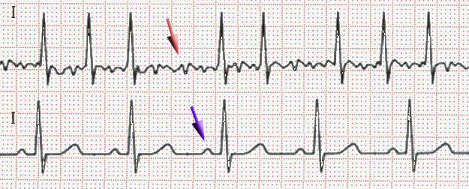
\includegraphics[scale=0.5]{Afib_ecg.jpg}
		\caption{Απεικόνιση κολπικής μαρμαρυγής \en \protect\url{https://commons.wikimedia.org/}}
	\end{figure}
	Ανάλογα με τη διάρκειά της χωρίζεται σε: παροξυσμική, κατά την οποία ο ασθενής επανέρχεται αυτόνομα σε διάστημα 7 ημερών, διαρκή ή επίμονη, στις περιπτώσεις που η μαρμαρυγή διαρκεί περισσότερο από 7 ημέρες. Σε αυτή την περίπτωση χρειάζεται εξωτερική παρέμβαση. Η κατάσταση αυτή μπορεί εν τέλει να οδηγήσει σε αναδιαμόρφωση των καρδιακών μυοκυττάρων προκαλώντας εν τέλη μυοκαρδιοπάθεια. Αυτός ο τύπος κολπικής μαρμαρυγής παρουσιάζεται τόσο ως ένα αρχικό επεισόδιο της πάθησης όσο και ως επαναλαμβανόμενο ενός περιστατικού παροξυσμικής μαρμαρυγής. Ακόμα δύο κατηγορίες είναι η: μακροχρόνια επίμονη κολπική μαρμαρυγή, όταν τα περιστατικά συμβαίνουν σε διάστημα 12 μηνών (σε αυτές τις περιπτώσεις έχει αποτύχει η φαρμακευτική αγωγή ή η όποια διαφορετική ιατρική παρέμβαση) και η μόνιμη κολπική μαρμαρυγή, περίπτωση στην οποία έχει εγκαταλειφθεί η οποιαδήποτε θεραπεία λόγω έλλειψης ανταπόκρισης του καρδιακού ρυθμού. 
	\par
	Η κολπική μαρμαρυγή χαρακτηρίζεται ως υποτροπιάζουσα όταν κάποιος ασθενής βιώνει δύο ή/και παραπάνω επεισόδια.
	\par 
	Παράγοντες αυξημένου κινδύνου για την κολπική μαρμαρυγή αποτελούν η προχωρημένη ηλικία, υποκείμενα καρδιακά νοσήματα και παθήσεις, ενδοκρινείς παθήσεις όπως ο υπερθυροειδισμός και ο διαβήτης, γενετικοί παράγοντες, νευρολογικές παθήσεις, φλεγμονές όπως η μυοκαρδίτιδα, υψηλή αρτηριακή πίεση καθώς και η υψηλή κατανάλωση αλκοόλ.
	\par
	Παρόλους τους κινδύνους που εγκυμονεί η κολπική μαρμαρυγή, έχουν αναπτυχθεί τεχνικές και θεραπείες που μειώνουν τις πιθανότητες εγκεφαλικού σε ασθενείς που πάσχουν από αυτήν. 
	Οι θεραπείες περιλαμβάνουν αντιπηκτικά φάρμακα, αγωγή για τον έλεγχο του καρδιακού ρυθμού και κάποιες παρεμβατικές διαδικασίες. [18]-[23], [29], [37], [40] 
	\begin{figure}[h]
		\centering
		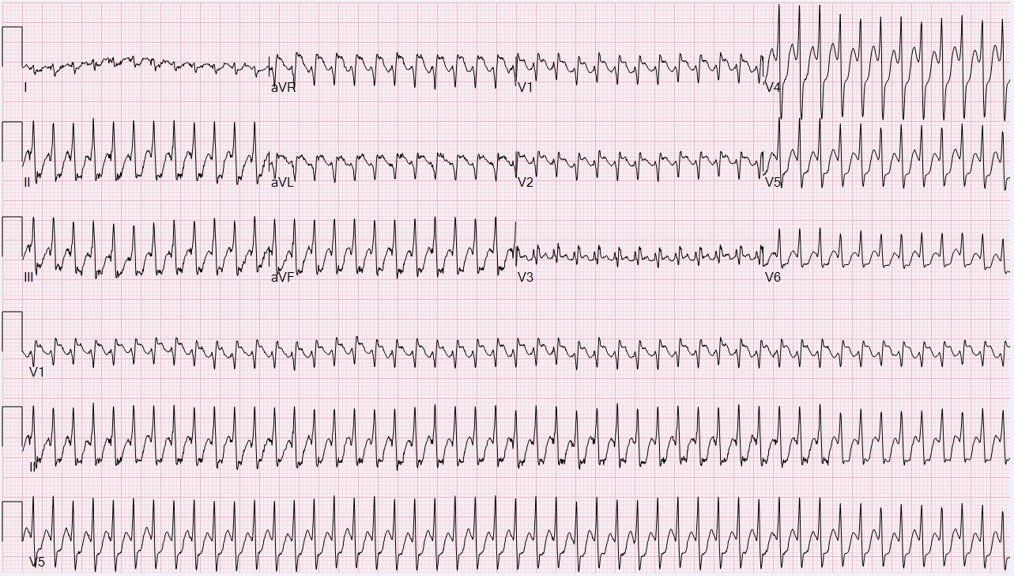
\includegraphics[scale=0.2]{Atrial_Flutter.jpg}
		\caption{Κολπικός πτερυγισμός \en\protect\url{https://commons.wikimedia.org/}}
	\end{figure}
	
	\item Κολπικός πτερυγισμός (\en Atrial flutter). \gr Ο όρος πτερυγισμός πηγάζει από μια οδοντωτή εικόνα κατά την καταγραφή του ΗΚΓ, που αντιστοιχεί σε ραγδαίο κολπικό ρυθμό, σε αντίθεση με τον ακανόνιστο ρυθμό της κολπικής μαρμαρυγής. Τα αίτια του κολπικού πτερυγισμού είναι όμοια με αυτά της κολπικής μαρμαρυγής και σε αρκετές περιπτώσεις φαινόμενα πτερυγισμού εναλλάσσονται με φαινόμενα μαρμαρυγής. Παρόλα αυτά, το 80 τοις εκατό των περιπτώσεων πτερυγισμού εμφανίζονται σε ασθενείς αρσενικού φύλου.
	\par
	Επίσης, ο πτερυγισμός χωρίζεται σε παροξυσμικό και επίμονο, ο οποίος σε πολλές περιπτώσεις χρίζει ιατρικής επέμβασης. Η απώλεια επαρκής σύσπασης των κόλπων και ο υψηλός καρδιακός ρυθμός μπορεί να οδηγήσει σε υπόταση, κυνάγχη, καρδιακή ανεπάρκεια ή συγκοπή. Σε αρκετές περιπτώσεις ο πτερυγισμός παραμένει ασυμπτωματικός για εβδομάδες και η εμμένουσα ταχυκαρδία μπορεί να καταλήξει σε καρδιακή ανεπάρκεια. Παρόλο που η κολπική λειτουργία μπορεί να επανέλθει στα φυσιολογικά επίπεδα, η αρρυθμία εμμένει και μπορεί να οδηγήσει σε αιφνίδιο θάνατο. \en [30]-[31]\gr
	\item Κολπική ταχυκαρδία \en (Atrial tachycardia). \gr Η κολπική ταχυκαρδία αφορά ηλεκτρικές ώσεις που παράγονται και παραμένουν εντός των κόλπων. Εμφανίζεται σε καταστάσεις υψηλών μεταβολικών απαιτήσεων και άγχους, όπως η υποξία, παρόλα αυτά αποτελεί καλοήθη αρρυθμία. Διαφέρει από την κολπική μαρμαρυγή και τον κολπικό πτερυγισμό και χρίζει ειδικής διάγνωσης ώστε να αποβεί σε σωστή διαχείρηση και θεραπεία. Προκαλείται από ένα ή παραπάνω μηχανισμούς που μπορούν να οδηγήσουν σε αρρυθμίες. Πολλές φορές ο μηχανισμός παραμένει απροσδιόριστος. Χωρίζεται σε τέσσερις διαφορετικές κατηγορίες: καλοήθης (εντοπίζεται συνήθως σε άτομα προχωρημένης ηλικίας. Είναι σύντομη, παροξυσμική και ο καρδιακός ρυθμός κυμαίνεται από 80 έως 140  παλμούς το λεπτό), πολυεστιακή (πολλαπλές ταυτόχρονες εκφορτίσεις του καρδιακού μυ, επηρεάζει μορφολογικά το έπαρμα Ρ και το διάστημα \en PR. \gr Συνήθως παρατηρείται σε συνδυασμό με χρόνια πνευμονική νόσο), κολπική ταχυκαρδία με αποκλεισμό (συνήθως ο κολπικός ρυθμός δεν επηρεάζεται. Αν και συνήθως αναφέρεται ως παροξυσμική, διατηρείται) και αδιάκοπη (σπάνια καρδιακή πάθηση τόσο σε παιδιά όσο και σε ενήλικες. Μοιάζει με φλεβοκομβική ταχυκαρδία και ο ρυθμός της κυμαίνεται στους 100-160 παλμούς το λεπτό). \par
	Πηγάζει συνήθως από κάποια έκτοπη σύσπαση και παράγει κολπικό ρυθμό 150-250 παλμούς το λεπτό, τα επάρματα Ρ δεν επηρεάζονται πάντα μορφολογικά. 
	Η κολπική ταχυκαρδία εμφανίζεται συνήθως σε άτομα με δομικές καρδιακές παθήσεις αλλά και ισχαιμική στεφανιαία νόσο. Ίσο βαθμό κινδύνου διατρέχουν και οι ασθενείς χωρίς δομικές νόσους και παθήσεις. Άλλα πιθανά αίτια αποτελούν οι πνευμονοπάθειες, το αλκόολ, διεγερτικά όπως οι ναρκωτικές ουσίες, η σοκολάτα και οι μεταβολικές αναταραχές. [36]-[39]  
	\begin{figure}[h]
		\centering
		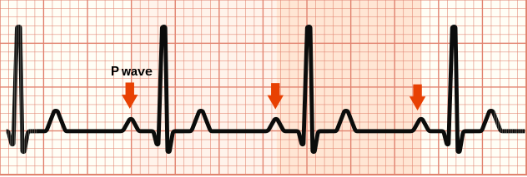
\includegraphics[scale=0.4]{normal.png}
		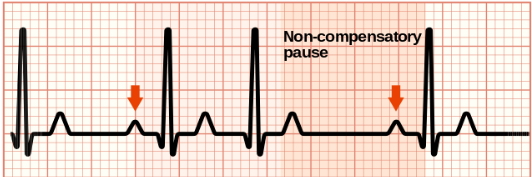
\includegraphics[scale=0.4]{pac.png}
		\caption{Εκτοπες κολπικές συσπάσεις. Στην πρώτη εικόνα (αριστερά) παρουσιάζεται ένας φυσιολογικός καρδιακός ρυθμός και στη δεύτερη (δεξιά) οι έκτοπες κολπικές συσπάσεις \en\protect\url{https://commons.wikimedia.org/}}
	\end{figure}
	\item Πρόωρη κολπική σύσπαση ή έκτακτη κολπική σύσπαση \en (Atrial premature complex or Premature Atrial Contractions - PAC). \gr  Πρόκειται για συσπάσεις που ξεκινούν από τους κόλπους αλλά δεν προέρχονται από το φλεβόκομβο, επηρεάζοντας τη μορφολογία του Ρ επάρματος. Το ρόλο του βηματοδότη αναλαμβάνει κάποιο άλλο τμήμα των κόλπων αλλά όχι ο φλεβόκομβος (μπορεί να επεμβαίνουν περισσότερα από ένα τμήματα). Συνήθως έχουν φυσιολογικό \en QRS \gr σύμπλεγμα και κανονικό, συντομότερο ή και μεγαλύτερο Ρ κύμα το οποίο είναι έκτοπο (δηλαδή συμβαίνει νωρίτερα από το φυσιολογικό). Το διάστημα \en PR \gr μπορεί να είναι ελαφρώς μεγαλύτερο. Συγκριτικά με το Ρ κύμα των φυσιολογικών συσπάσεων, το Ρ κύμα των υπερκοιλιακών αρρυθμιών διαφέρει ως προς τη μορφολογία και προηγείται χρονικά. Συνήθως ένα φυσιολογικό Ρ έπαρμα προηγείται της ενεργοποίησης των κοιλιών. Όταν το πρόωρο Ρ κύμα συμβαίνει σχετικά κοντά στο φυσιολογικό χτύπο, η μορφολογία του Ρ κύματος που παράγεται είναι ενδιάμεση του φυσιολογικού αλλά και του έκτοπου παλμού. Μπορεί να συμβαίνουν σε ζεύγη, να ακολουθούν προηγούενο \en PAC \gr, να συμβαίνουν μετά από κάθε ένα, δύο ή τρεις συνεχόμενους φυσιολογικούς παλμούς δημιουργώντας μοτίβα. Αν συμβούν αρκετά πρόωρα, μπορεί να προκαλέσουν τη δημιουργία ενός πιο πεπλατυσμένου \en QRS \gr συμπλέγματος. Οι αιτίες εμφάνισής τους μπορεί να συνδέονται με τη δομή της καρδιάς (υπερτροφική καρδιομυοπάθεια) είτε με χημικούς παράγοντες (αγωνιστές των β-υποδοχέων). Οι λόγοι που τις πυροδοτούν είναι ιδιοπαθείς, δηλαδή ποικίλοι, συχνά εμφανίζονται αυθόρμητα και η αιτία τους παραμένει άγνωστη. Οι ιδιοπαθείς πρόωρες κολπικές συσπάσεις συχνά ξεκινούν από πνευμονικές φλέβες όταν δεν υπάρχει κάποια δομική καρδιακή πάθηση. Οι αιτίες πρόκλησής τους μπορούν να ερμηνευθούν ως δομικές, χημικές ή κάποιο αποτέλεσμα διαφορετικού συνόλου καταστάσεων ή παθήσεων. Αν οι κόλποι αδυνατούν να προκαλέσουν σύσπαση, ο παλμός σταματά (δεν μπορεί να αντληθεί αίμα). Όταν υπάρχουν τρεις ή περισσότερες έκτακτες κολπικές συστολές το σήμα ερμηνεύεται ως κολπική ταχυκαρδία.
	\par
	Εντοπίζονται τόσο σε νέους ασθενείς όσο και σε γηραιότερους. Οι δομικές αιτίες τους συμπεριλαμβάνουν παθήσεις όπως η στεφανιαία νόσος, η υπερτροφική μυοκαρδιοπάθεια, τα ανευρύσματα του αριστερού κόλπου, η υπερτροφία της αριστερής κοιλίας αλλά και συγγενείς καρδιακές δυσπλασίες. Συγγενή συμπτώματα έχουν εμφανιστεί ακόμα και σε βρέφη και συνήθως τα αίτια θεωρούνται παθολογικά. Παρόλα αυτά η ανίχνευσή και ο εντοπισμός τους είναι πιο πιθανό να συμβούν κατά συνεχή καταγραφή με κάποιον καταγραφέα \en Holter \gr από ότι κατά την καταγραφή ενός ΗΚΓ. Οι επιλοκές, τέλος, που μπορούν να προκαλέσουν οφείλονται στους παράγοντες που ευθύνονται για την εμφάνισή τους. Μερικά παραδείγματα επιπλοκών είναι η κολπική μαρμαρυγή και τα ισχαιμικά εγκεφαλικά επεισόδια. Μεμονωμένες συσπάσεις δε συμβάλλουν σε αυξημένες πιθανότητες καρδιακών επεισοδίων και θανάτου. [27], [36], [37] \en
\end{itemize}
\begin{figure}[h]
	\centering
	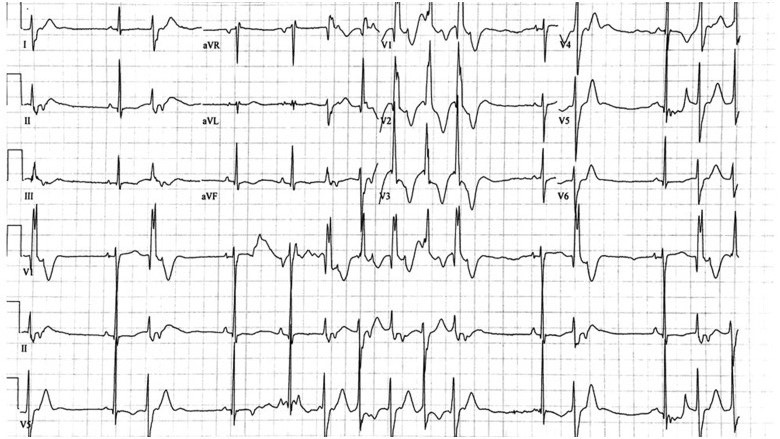
\includegraphics[scale=0.3]{ventricular tachycardia.jpg}
	\caption{Κοιλιακή ταχυκαρδία \en\protect\url{https://en.wikipedia.org/}}
\end{figure}
\subsubsection{Κοιλιακή αρρυθμία} 
Οι κοιλιακές ταχυκαρδίες αποτελούν ταχυπαλμίες που ξεκινούν στις κοιλίες της καρδιάς και είναι εξαιρετικά επικίνδυνες (110-250 χτύποι το λεπτό). Το \en QRS \gr σύμπλεγμα διαρκεί σημαντικά μεγαλύτερο διάστημα και ποικίλει σε μορφολογία. Μερικοί από τους πιθανούς τύπους εμφάνισης αποτελούν: δύο διαφορετικοί τύποι \en QRS \gr συμπλέγματος που εναλλάσσονται μεταξύ τους, περισσότεροι από δύο τύποι \en QRS \gr που εμφανίζονται στο καρδιογράφημα ή σταδιακή εναλλαγή των \en QRS \gr συμπλεγμάτων σε σχήμα και διάρκεια από μη φυσιολογικό σε φυσιολογικό. Ανάλογα με το χρονικό σημείο του παλμού κατά το οποίο εμφανίζονται, το αποτέλεσμα ποικίλει από κοιλιακή μαρμαρυγή (μη συγχρονισμένη σύσπαση διαφορετικών τμημάτων της καρδιάς), ταχυκαρδία (τρεις ή περισσότερες συνεχόμενες συστολές) ή κοιλιακό πτερυγισμό (παρουσιάζοντας μια πριονωτή εικόνα) διαταραχές οι οποίες μπορεί να αποβούν θανατηφόρα. Η στεφανιαία νόσος, το έμφραγμα του μυοκαρδίου, η αποδυνάμωση του καρδιακού μυ και άλλες παθήσεις μπορεί να προκαλέσουν κοιλιακές αρρυθμίες. H προέλευσή της βρίσκεται χαμηλότερα του κολποκοιλιακού κόμβου.
\begin{itemize}
	\item  Έκτακτη κοιλιακή συστολή, \en Premature Ventricular Contractions (PVC)\gr : Αποτελεί πρόωρη εκπόλωση του μυοκαρδίου που ξεκινά από τις κοιλίες και δημιουργεί μια επιπλέον (μη φυσιολογική) σύσπασή τους. Χαρακτηρίζονται από πρώιμο \en QRS \gr σύμπλεγμα με ανώμαλη μορφολογία και χρονική διάρκεια μεγαλύτερη των 120 \en msec \gr . Ανάλογα με ποιο τμήμα των κοιλιών συσπάται δημιουργείται και ένα διαφορετικό (μη φυσιολογικό) \en QRS \gr σύμπλεγμα. Ακολουθούνται από ένα εκτενές Τ κύμα χωρίς την ύπαρξη προηγούμενων (έκτοπων) Ρ κυμάτων και η μορφολογία των τελευταίων παραμένει ίδια. Εμφανίζονται οποιαδήποτε στιγμή του καρδιακού κύκλου και παρατηρούνται μεμονωμένα, σε ζεύγη ή έπειτα από κάθε ένα, δύο, τρεις ή και τέσσερις φυσιολογικούς παλμούς (δημιουργώντας διαφορετικά μοτίβα). Σε πολλές περιπτώσεις εμφανίζονται σε συνδυασμό με δομικές καρδιακές παθήσεις, ωστόσο παρατηρούνται και ανεξάρτητα από αυτές. 
	\par
	Κατά τη διάρκεια μιας έκτοπης κοιλιακής συστολής ο παλμός ξεκινάει από τις ίνες \en Purkinje \gr (κύτταρα υπέυθυνα για δημιουργία ηλεκτρικών ώσεων) αντί για το φλεβόκομβο. Οι πρόωρες κοιλιακές συστολές προηγούνται ενός φυσιολογικού παλμού και ο επόμενος φυσιολογικός παλμός φαίνεται να καθυστερεί, καθώς συμβαίνει μετά από μια παύση. Επιπλεόν, οι συστολές αυτές μπορούν να εμφανιστού μεμονωμένα αλλά και σε μοτίβα των δύο ή τριών συνεχόμενων παλμών· περισσότερες από τρεις συνεχόμενες συστολές αυτού του τύπου κατηγοριοποιούνται ως κολπική ταχυκαρδία.
	\par
	Στην περίπτωση που αυτού του τύπου παλμοί εναλλάσσονται συνεχώς με φυσιολογικό παλμό, ο ασθενής βρίσκεται σε κατάσταση διδυμίας \en (bigeminy).\gr Ομοίως όταν ένας φυσιολογικός παλμός μεσολαβεί μετά από δύο έκτοπες κοιλιακές συστολές ο ασθενής βρίσκεται σε τριδυμία \en (trigeminy).\gr  Όταν ανιχνεύεται στο ΗΚΓ η ύπαρξη τριών ή περισσότερων συνεχόμενων συστολών, η διάγνωση συνήθως είναι κοιλιακή ταχυκαρδία. Περαιτέρω, η αρρυθμία θεωρείται παρατεταμένη αν διαρκεί πάνω από τριάντα δευτερόλεπτα και μη παρατεταμένη στην αντίθετη περίπτωση.
	\par 
	Η πλειοψηφία αυτών των συστολών συμβαίνουν αυθόρμητα και οι αιτίες προέλευσής τους δεν είναι γνωστές. Καταστάσεις και παράγοντες που μπορεί να εντείνουν την κατάσταση είναι η ακατάσχετη κατανάλωση καφεΐνης, τα υψηλά επίπεδα στρες, η κατανάλωση αλκοόλ, ναρκωτικών ουσιών και καπνού και η έλλειψη ύπνου. Γίνονται αντιληπτές με την αίσθηση έντονων παλμών στο στήθος των ασθενών αλλά στις περισσότερες περιπτώσεις είναι καλοήθεις και δε χρίζουν αγωγής. Πιο συγκεκριμένα, η αίσθηση μοιάζει με έλλειψη ενός παλμού και στη συνέχεια η αίσθηση φτερουγίσματος. Τέλος, μερικοί ασθενείς βιώνουν ζαλάδες, δυσφορία, στηθάγχη και πιο σπάνια συγκοπή. 
	\par
	Από δομικής άποψης, οι παθήσεις/αδυναμίες που μπορούν να οδηγήσουν στην εφάνιση των έκτοπων κοιλιακών συστολών είναι όσες έχουν ως αποτέλεσμα τη μεταβολή των οδών αγωγιμότητας λόγω αλλοιώσεων των ιστών. Όσον αφορά βιολογικές παθήσεις μη σχετικές με την καρδιά, αυτές που θεωρούνται σχετικές με την εμφάνιση των έκτοπων συστολών είναι η αναιμία και ο υπερθυρεοειδισμός.
	\par 
	Τέλος, εξαιτίας της μειωμένης συχνότητας εμφάνισής τους, δεν ανιχνεύονται εύκολα μέσω ΗΚΓ, κάτι το οποίο τις διαφοροποιεί από τις αντίστοιχες κολπικές συστολές. Αυτά που το ΗΚΓ μπορεί να ανιχνεύσει είναι "μυτερά" Τ επάρματα, επιμήκυνση \en QRS \gr συμπλέγματος ή απώλεια \en R \gr επάρματος.
	
	Όσον αφορά τον κοιλιακό πτερυγισμό και την κοιλιακή ταχυκαρδία, αποτελούν αρρυθμίες αντίστοιχες με τις ομώνυμες κολπικές. Η κοιλιακή ταχυκαρδία απαιτεί άμεση αντιμετώπιση διότι συχνά οδηγεί σε κοιλιακή μαρμαρυγή και ανακοπή. Σε μερικές περιπτώσεις μια ενέργεια που μπορεί να σταματήσει την ταχυκαρδία είναι μια δυνατή γροθιά στο στέρνο. [27], [33], [34]
	
	\item  Κοιλιακή ταχυκαρδία (\en Ventricular tachycardia). \gr μπορεί να είναι παρατεταμένη αν διαρκέσει περισσότερο από τριάντα δευτερόλεπτα ή αν δημιουργήσει κατάσταση στην οποία χρειάζεται εξωτερική παρέμβαση. Ακόμα μπορεί να είναι μη παρατεταμένη, δηλαδή να διαρκέσει λιγότερο από τριάντα δευτερόλεπτα, μη δημιουργώντας κάποια αστάθεια. Τα συμπτώματα αυτής της ταχυκαρδίας εκτείνονται σε ένα ευρύ φάσμα, όπως αισθητά έντονοι παλμοί, στηθάγχη, αδυναμία φυσιολογικής αναπνοής και καρδιακή ανακοπή [32], [34].
	\par
	\item Κοιλιακή μαρμαρυγή (\en Ventricular fibrillation\gr). Κατηγοριοποιείται ως τύπος αρρυθμίας που επηρεάζει τη μορφολογία του \en QRS \gr συμπλέγματος, επιμηκύνοντάς το. Εμφανίζεται όταν τμήματα του κοιλιακού μυοκαρδίου εκπολώνονται ακανόνιστα και με ασυντόνιστο τρόπο. Απεικονίζεται στο ΗΚΓ με κοιλιακό ρυθμό υψηλότερο του 300 και με διακριτά \en QRS \gr συμπλέγματα. Γενικότερα, ο ρυθμός ειναι ακανόνιστος και η μορφολογία του \en QRS \gr συμπλέγματος διαφέρει στο μήκος, το σχήμα και το πλάτος. Είναι εξαιρετικά επικίνδυνη και μπορεί να οδηγήσει σε καρδιακή ανακοπή. Η κοιλιακή μαρμαρυγή έχει παρατηρηθεί στο εβδομήντα τοις εκατό των θανάτων από καρδιακή ανακοπή. Οι παθήσεις που συνδέονται με την κοιλιακή μαρμαρυγή σχετίζονται με ανωμαλίες ηλεκτρολυτών (υποκαλιαιμία/υπερκαλιαιμία, υπομαγνησιαιμία), οξέωση, υποθερμία, υποξία, μυοκαρδιοπάθειες, οικογενειακό ιστορικό αιφνίδιου καρδιακού θανάτου και χρήση αλκοόλ.
	\par
	Κατά την εμφάνιση της κοιλιακής μαρμαρυγής, οι ασθενείς εμφανίζουν συμπτώματα εμφράγματος του μυοκαρδίου (δυσκολία αναπνοής, τάση προς εμετό και ναυτία πριν το συμβάν). Στην περίπτωση στεφανιαίας νόσου ή καρδιακής ανεπάρκειας τα συμπτώματα επιδεινώνονται (κυνάγχη, έντονη δύσπνοια και  οξεία νυχτερινή δύσπνοια). Κατά την εμφάνισή της οι ασθενείς δεν έχουν τις αισθήσεις τους και ο παλμός τους δεν είναι αισθητός. Εάν δεν υπάρξει άμεση δράση, μπορεί να οδηγήσει σε θάνατο σε μερικά λεπτά.
	\par
	Όσον αφορά τη μορφολογική απεικόνιση, παρατηρούνται αποκλίσεις από τη γραμμή βάσης του ΗΚΓ, με ποικιλία στο πλάτος και το σχήμα, δεν υπάρχει διάκριση των κύριων επαρμάτων (Ρ και Τ) όυτε και του \en QRS \gr συμπλέγματος και ο καρδιακός ρυθμός κυμαίνεται από εκατό έως εκατόν πενήντα παλμούς το λεπτό. [33]
	\par
	Συμπτώματα που βιώνουν οι ασθενείς είναι: πόνος στο στήθος, δύσπνοια, ναυτία και έμετος. Κατά τη διάρκεια εξέλιξής της οι ασθενείς είναι συχνά αναίσθητοι και ο παλμός τους δεν είναι ανιχνεύσιμος. Ακόμα και αν αντιμετωπιστεί εγκαίρως, συχνά αφήνει νευρολογικά κατάλοιπα [33]. 
	\begin{figure}
		\centering
		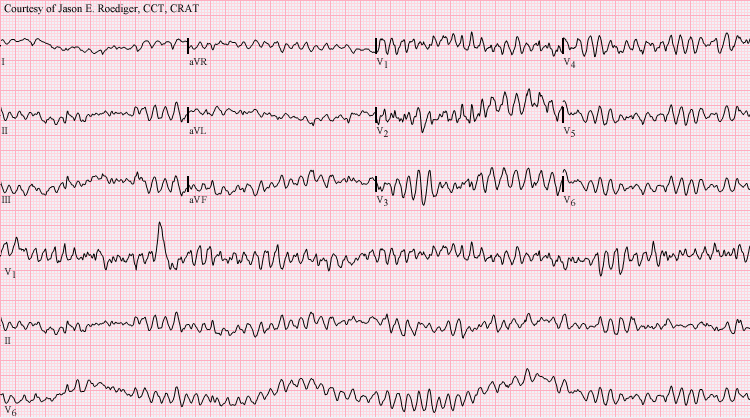
\includegraphics[scale=0.3]{Ventricular_fibrillation.png}
		\caption{Κοιλιακή μαρμαρυγή \en \protect\url{en.wikipedia.org}}
	\end{figure}
	
	
	\begin{figure}[h]
		\centering
		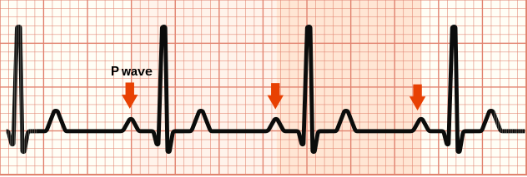
\includegraphics[scale=0.4]{normal.png}
		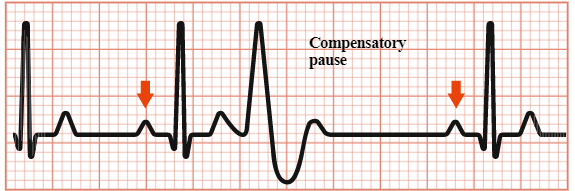
\includegraphics[scale=0.38]{pvc.png}
		\caption{Εκτοπες κοιλιακές συσπάσεις. Στην πρώτη εικόνα (αριστερά) παρουσιάζεται ένας φυσιολογικός καρδιακός ρυθμός και στη δεύτερη (δεξιά) οι έκτοπες κοιλιακές συσπάσεις \en\protect\url{commons.wikimedia.org}}
	\end{figure}
\end{itemize}

\subsubsection{Κομβική αρρυθμία} 
Ο φλεβόκομβος είναι ο βασικός βηματοδότης της καρδιάς και εντοπίζεται στον άνω δεξιό κόλπο της. Ένας δεύτερος βηματοδότης είναι ο κολποκοιλιακός κόμβος και βρίσκεται στον κάτω δεξιό κόλπο. Η δέσμη \en His \gr αποτελεί έναν τρίτο καρδιακό βηματοδότη που βρίσκεται στο όριο ανάμεσα στους κόλπους και τις κοιλίες (συλλογή μυϊκών καρδιακών κυττάρων υπέυθυνων για ηλεκτρικές ώσεις). Ο κομβικός ρυθμός είναι ένας μη φυσιολογικός καρδιακός ρυθμός ο οποίος ξεκινά από τον κολποκοιλιακό κόμβο ή τη δέσμη \en His. \gr Ο ρυθμός αυτός μεταβάλλεται ως εξής: κομβική βραδυκαρδία, όταν ο ρυθμός είναι χαμηλότερος από 40 χτύπους το λεπτό, ρυθμός διαφυγής διασταύρωσης (40-60 παλμούς ανά λεπτό), επιταχυνόμενος κομβικός ρυθμός (60-100 παλμούς ανά λεπτο) και κομβική ταχυκαρδία (περισσότεροι από 100 παλμοί ανά λεπτό). 
\par
Στις περιπτώσεις που η λειτουργία του φλεβόκομβου εμποδίζεται, δημιουργείται ένας κομβικός ρυθμός. Η κατάσταση αυτή μπορεί να προκληθεί από πολυάριθμες καταστάσεις αλλά και φάρμακα. Μερικές τέτοιες καταστάσεις είναι πόνος στο στήθος, ακτινοθεραπεία, μυοκαρδίτιδα, λίθιο, οπιοειδή και κανναβινοειδή.  Τέλος, η αγωγή εξαρτάται κατά κύριο λόγο από τις υποκείμενες αιτίες και νοσήματα.  [42], [43]
‌

\subsubsection{Υπερκοιλιακή αρρυθμία} Ονομάζεται έτσι διότι συμβαίνει στα σημεία άνω του κολποκοιλιακού κόμβου.
\par
Η υπερκοιλιακή αρρυθμία \en (Supraventricular arrhythmia, SVT)\gr προκαλεί στα άτομα που τη βιώνουν έντονη δυσφορία. Μπορεί να εντοπιστεί κατά τη διάρκεια ηλεκτροκαρδιογραφήματος. Η αναλογία ανάμεσα στους άντρες και τις γυναίκες που επηρεάζονται έιναι 1:2 σε όλες τις ηλικίες. Οι βασικές κατηγορίες της είναι η κολποκοιλιακή ταχυκαρδία επανεισόδου, κολποκοιλιακή κομβική ταχυκαρδία επανεισόδου και κολπική ταχυκαρδία, με τη δεύτερη να εμφανίζεται πιο συχνά. Πολύ συχνά, τα επάρματα Ρ δεν είναι εμφανή κατά το ΗΚΓ εξαιτίας της ταυτόχρονης διέγερσης των κόλπων και των κοιλιών και στις περιπτώσεις που διακρίνονται είναι ανεπαίσθητα (ψευδοέπαρμα Ρ). [44]
\par
\textbf{Κολποκοιλιακή κομβική ταχυκαρδία επανεισόδου \en (AVNRT)} \gr \par
\gr Η κολποκοιλιακή κομβική ταχυκαρδία επανεισόδου \en (AVNRT) \gr αποτελεί παροξυσμική υπερκοιλιακή ταχυκαρδία που προκύπτει εξαιτίας κυκλώματος επανεισόδου εντός ή δίπλα στον κολποκοιλιακό κόμβο. Η διάγνωσή της εντοπίζεται κατά τη διάρκεια ΗΚΓ. Στην πλειοψηφία, το ΗΚΓ θα δείξει καρδιακό ρυθμό ανάμεσα σε 140 και 280 παλμών ανά λεπτό και ένα σύμπλεγμα \en QRS \gr μικρότερο από 120 χιλιοστά του δευτερολέπτου. 
\par
Τα συμπτώματα περιλαμβάνουν ζαλάδα, συγκοπή, δύσπνοια, δυσφορία γύρω από το λαιμό και σε άτομα με ιστορικό στεφανιαίας νόσου ακόμα και συμπτώματα εμφράγματος. Η συγκοπή είναι τυπική σε ασθενείς με καρδιακό ρυθμό πάνω από 170 παλμούς το λεπτό, καθώς μικρότερη αιμάτωση των κοιλιών οδηγεί σε μείωση  καρδιακής ικανότητας και μειωμένη αιμάτωση του εγκεφάλου. [35] 
\par

\begin{figure}[h]
	\centering
	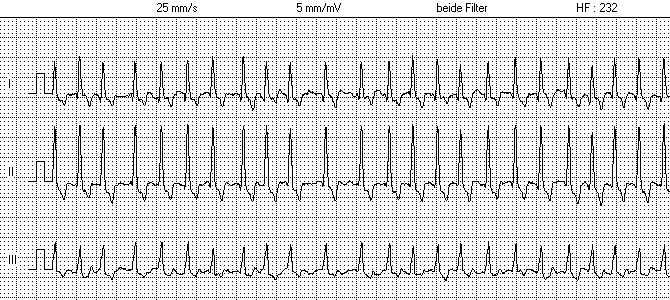
\includegraphics[scale=0.3]{supraventricular tachychardia.jpg}
	\caption{Υπερκοιλιακή ταχυκαρδία \en\protect\url{en.wikipedia.org}}
\end{figure}
\subsection{Με βάση τον καρδιακό ρυθμό}
\subsubsection{Ταχυαρρυθμία η ταχυκαρδία \en (Tachyarrhythmia)} 
Oρίζεται ως αποκλίνων καρδιακός ρυθμός με τουλάχιστον 100 παλμούς το λεπτό. Χωρίζεται με τη σειρά του με βάση το σημείο προέλευσης της αρρυθμίας σε : 

\subsubsection{Βραδυαρρυθμία ή βραδυκαρδία \en (Bradyarrhythmia) \gr}
Κατάσταση κατά την οποία ο καρδιακός ρυθμόε είναι ίσος ή χαμηλότερος των 60 παλμών ανά λεπτό. Συμπεριλαμβάνει διαφορετικές ρυθμικές διαταραχές, οι οποίες παρουσιάζονται στη συνέχεια. Εάν ο ρυθμός μειωθεί σε μεγάλο βαθμό, η παροχή αίματος στον εγκέφαλο περιορίζεται με αποτέλεσμα τη λιποθυμία.
\par
Ο φλεβόκομβος είναι βασικός βηματοδότης της καρδιάς, αποκτώντας με αυτό τον τρόπο σημαντικό ρόλο στην κυκλοφορία του αίματος και τη λειτουργία του μυοκαρδίου. Η φλεβοκομβική βραδυκαρδία αποτελεί ένα καρδιακό ρυθμό κατά τον οποίο αν και οι παλμοί είναι χαμηλότεροι του φυσιολογικού δεν υπάρχει κάποια δομική αδυναμία ή ανωμαλία. Μπορεί να διαγνωστεί μέσω ΗΚΓ και η απεικόνιση είναι αυτή ενός φυσιολογικού καρδιακού ρυθμού σε μορφολογία αν και είναι χαμηλότερος. Εμφανίζεται κυρίως σε άτομα άνω των 65 και σε νεόυς αθλητές.
\par
Οι αιτίες της βραδυκαρδίας είναι τόσο εσωτερικές όσο και εξωτερικές. Οι εσωτερικές μπορεί να είναι τραύμα στο στήθος, έμφραγμα του μυοκαρδίου, στεφανιαία νόσος, μυοκαρδίτιδα, νόσος του \en Lyme \gr και πολλές ακόμα. Κύριες εξωγενείς αιτίες αποτελούν κυρίως φαρμακευτικές αγωγές όπως οι β-αναστολείς και στη συνέχεια η χρήση ναρκωτικών ουσιών και τα κανναβινοειδή, ο υποθυρεοειδισμός, η άπνοια, ακόμα και η νευρική ανορεξία. 
\par
\begin{figure}
	\centering
	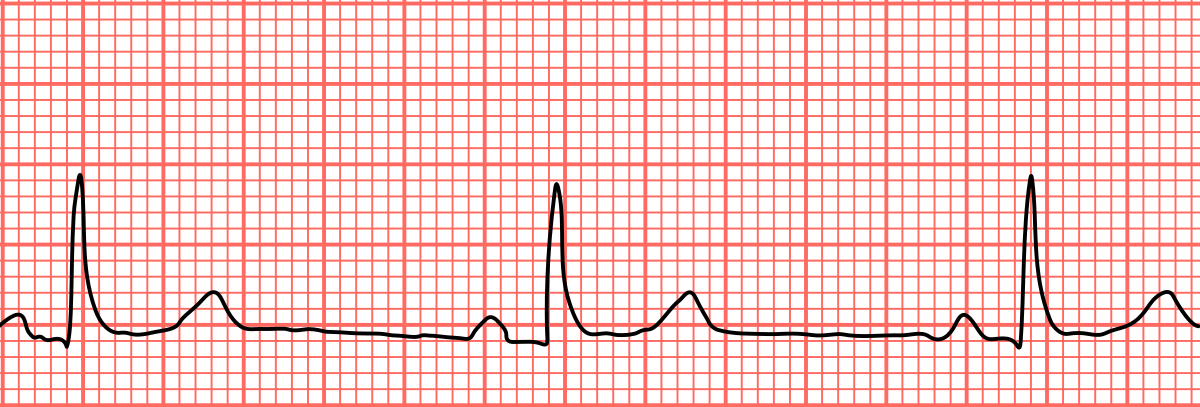
\includegraphics[scale=0.2]{bradychardia.png}
	\caption{Βραδυκαρδία \en\protect\url{en.wikipedia.org}}
\end{figure}
Η πλειοψηφία των ασθενών με βραδυκαρδία δεν παρουσιάζουν κάποια συμπτώματα. Υγιείς ενήλικες νεαρής ηλικίας και αθλητές σε κατάσταση ηρεμίας εμφανίζουν βραδυκαρδία λόγω του αυξημένου πνευμονογαστρικού τόνου (\en increased vagal tone),\gr γεγονός που δηλώνει αυκημένη καρδιακή μεταβλητότητα. Βραδυκαρδία εμφανίζεται και σε ενήλικες άνω των 65 σε κατάσταση ύπνου, που οφείλεται στη γήρανση του φλεβόκομβου [18]-[26], [40], [41]. 
\par

%\end{document}

\newpage
%
\gr
\chapter{Εκτίμηση μεταβλητότητας καρδιακού ρυθμού}
\section{Μετρικές εκτίμησης μεταβλητότητας καρδιακού ρυθμού}
Στο προηγούμενο κεφάλαιο παρουσιάστηκε ο ορισμός της καρδιακής μεταβλητότητας (\en Heart Rate Variability, HRV \gr) και η βαρύτητα που διαθέτει ως προς την αξιολόγηση της φυσιολογικής λειτουργίας της καρδιάς. Η αξιολόγηση και η μέτρηση αυτή πραγματοποιείται με χρήση διαφορετικών μετρικών. Οι δύο βασικές κατηγορίες μετρικών είναι οι γραμμικές και οι μη γραμμικές και στη συνέχεια οι γραμμικές μέθοδοι χωρίζονται σε δύο επιπλέον κατηγορίες, τις μετρικές στο χώρο του χρόνου και τις μετρικές στο χώρο της συχνότητας. Σε αυτό το κεφάλαιο θα αναλυθούν οι συγκεκριμένες μετρικές και η σημαντικότητά τους ως προς την αξιολόγηση του \en HRV. \gr
\subsection{Γραμμικές μέθοδοι}
\textbf{\\ Μέθοδοι στο πεδίο του χρόνου}
\par
Οι μετρικές στο πεδίο του χρόνου αντικατοπτρίζουν τη μεταβλητότητα ανάμεσα στους διαδοχικούς καρδιακούς παλμούς. Συνήθως εκφράζονται σε αρχικές μονάδες ή σε μορφή λογαρίθμου (πιο συγκεκριμένα του φυσικού λογαρίθμου \en ln() \gr για μια πιο κανονική κατανομή). 
\par
Το πλεονέκτημά του σε σύγκριση με αυτό της συχνότητας, είναι ότι οι μετρήσεις που παράγουν τους ανάλογους δείκτες γίνονται απευθείας επάνω στο σήμα και υπάρχει μόνο ένας τρόπος υπολογι\-σμού. Οι διάφοροι αυτοί δείκτες υπολογίζονται με βάση τα ονομαζόμενα ΝΝ-διαστήματα \en (NN intervals, N = normal), \gr  συνώνυμα των \en RR \gr διαστημάτων, με τη διαφορά ότι επιλέγονται μόνο Ν χτύποι, δηλαδή χτύποι που 
προέρχονται από εκπολώσεις του φλεβόκομβου. Οι δείκτες που προκύπτουν χωρίζονται σε δύο κατηγορίες, τη στατιστική και τη γεωμετρική.

\par
Στον παρακάτω πίνακα παρουσιάζονται σχεδιαγραμματικά οι μετρικές στο πεδίο του χρόνου και έπειτα η ανάλυση της κάθε μίας ξεχωριστά (Πίνακας 3.1).

\begin{center}
	\begin{longtable}{l l l}
		\caption{Μετρικές στο πεδίο του χρόνου} \\
		\centering 
		Όνομα παραμέτρου & Μονάδες μέτρησης & Περιγραφή \\ [0.5ex] 
		\endfirsthead
		\hline \hline \en 
		\en SDNN & \en $ms$ & Τυπική απόκλιση ΝΝ διαστημάτων \\ [1ex] 
		\en SDRR & \en $ms$ & Τυπική απόκλιση \en RR \gr διαστημάτων  \\ [1ex] 
		\en SDANN & \en $ms$ & Τυπική απόκλιση των μέσων \\ 
		& & διαστημάτων NN για \\
		& & κάθε τμήμα 5 λεπτών σε μια\\
		& & 24 ωρη καταγραφή \\ [1ex] 
		\en SDNN \\
		\en index \\
		\en (SDNNI) & \en $ms$ & Μέσος όρος των \\
		& & τυπικών αποκλίσεων όλων των \\ 
		& & διαστημάτων NN για κάθε τμήμα 5  \\
		& & λεπτών μιας 24 ωρης εγγραφής \\ [1ex] 
		\en pNN50 & $\%$ & Ποσοστό διαδοχικών διαστημάτων  \\
		& & \en RR \gr με χρονική διαφορά\\
		& & μεγαλύτερη των 50 \en ms\\ [1ex] 
		\en HR Max \& \\
		\en HR Min &\en $bpm$ & Μέση διαφορά μεταξύ των υψηλότερων \\
		& & και των χαμηλότερων καρδιακών \\
		& & παλμών κατά τη διάρκεια κάθε\\
		& & αναπνευστικού κύκλου \\ [1ex] 
		\en RMSSD & \en $ms$ & Τετραγωνική ρίζα διαδοχικών\\
		& & διαφορών διαστήματος \en RR\\ [1ex] 
		\en HRV \\
		\en triangular \\
		\en index & - & Ολοκλήρωμα της πυκνότητας \\
		& & του ιστογράμματος διαστήματος \en RR \gr \\
		& & διαιρεμένο με το ύψος του \\ [1ex] 
		\en TINN & \en $ms$ & Πλάτος βάσης του ιστογράμματος \\
		& & διαστήματος \en RR \gr \\ [1ex] 
		\hline 
	\end{longtable}
\end{center}

\begin{itemize}
	\item Στατιστικές μέθοδοι: Προκύπτουν από καταγραφές σημάτων μεγάλης διάρκειας που φτάνουν τις 24 ώρες. Οι τιμές τους αποκτώνται είτε από απευθείας μετρήσεις των ΝΝ διαστημάτων είτε μετά από επεξεργασία (αριθμητικές διαφορές ανάμεσα στις τιμές των διαστημάτων ΝΝ). Μερικοί από τους δείκτες που προκύπτουν χωρίς τη χρήση των διαφορών των διαστημάτων είναι οι
	\begin{itemize}
		\item \en SDNN
		\item SDANN \gr
	\end{itemize}
	Από τους πιο κοινούς δείκτες που προκύπτουν από διαφορά ανάμεσα σε ΝΝ διαστήματα είναι οι
	\begin{itemize}
		\item \en RMSSD
		\item SDNNi
		\item SDSD
		\item NN50 count
		\item pNN50 \gr
	\end{itemize}
	\item Γεωμετρικές μέθοδοι: Οι γεωμετρικές μέθοδοι χαρακτηρίζονται από μεγαλύτερη ανθεκτικότητα όσον αφορά στην ποιότητα των δεδομένων που συλλέγονται. Η διαφορά τους με τις στατιστικές μεθόδους είναι η διάρκεια των διαστημάτων των μετρήσεων, που φτάνουν έως και τα είκοσι λεπτά. Οι ακολουθίες των ΝΝ διαστημάτων μπορούν να μελετηθούν μέσω της μετατροπής τους σε γεωμετρικά μοτίβα. Τα μοτίβα που παράγονται μπορούν να προσεγγιστούν με δύο διαφορετικούς τρόπους. Ο πρώτος τρόπος είναι οι βασικές μετρήσεις των γεωμετρικών μοτίβων, παραδείγματος χάριν, εκτίμηση της μέγιστης τιμής του άξονα Χ ή \en Y \gr (π.χ. η τιμή του \en HRV triangular index \gr, δίνεται, μέσω του διαγράμματος της εικόνας, ως ο λόγος \en D/Y \gr). O δεύτερος τρόπος είναι η παρεμβολή μαθηματικού σχήματος στο γεωμετρικό μοτίβο, δηλαδή η προσέγγιση της κατανομής του ιστογράμματος με ένα τρίγωνο. Η αναγωγή αυτή, στη συνέχεια, χρησιμοποιείται για την εκτίμηση του ΤΙΝΝ (ΤΙΝΝ = Β-Α).
	Οι γεωμετρικές μέθοδοι χρησιμοποιούν την ακολουθία των ΝΝ διαστημάτων για τη μετατροπή, η οποία οδηγεί στη δημιουργία ιστογραμμάτων. Οι τέσσερις πιο συνηθισμένοι δείκτες μέτρησης των γεωμετρικών μεθόδων είναι οι: 
	\begin{itemize}
		\item \en HRV triangular index \gr: Προκύπτει από τη χρήση εικοσιτετράωρων μετρήσεων και ορίζεται ως το ολοκλήρωμα της πυκνότητας του ιστογράμματος των \en RR \gr διαστημάτων διαιρεμένο με το ύψος του ιστογράμματος.
		\item ΤΙΝΝ: Το πλάτος του ιστογράμματος των \en RR \gr διαστημάτων (μονάδα μέτρησης: \en $ms$).\gr
		\item \en Differential index: \gr Διαφορές του πλάτους του ιστογράμματος διαφορών ανάμεσα σε γειτονικά ΝΝ διαστήματα μετρημένα σε συγκεκριμένα ύψη (μονάδα μέτρησης: \en $ms$).\gr
		\item \en Logarithmic index \gr: Συντελεστής φ της αρνητικά εκθετικής καμπύλης \en k * e - \gr φ \en t.
	\end{itemize}
\end{itemize}
\gr
\textbf{\\ Μέθοδοι στο πεδίο της συχνότητας}
\par
Οι μέθοδοι στο πεδίο της συχνότητας εκτιμούν την κατανομή (απόλυτης και σχετικής) ισχύος σε τέσσερις βασικές ζώνες συχνότητας και οι καταγραφές κυμαίνονται σε διάρκεια είτε από 2-5 λεπτά είτε 24 ώρες. Οι ζώνες αυτές είναι ονομαστικά οι: υπέρ χαμηλές συχνότητες, πολύ χαμηλές συχνότητες, χαμηλές συχνότητες και υψηλές συχνότητες. Η κατηγοριοποίηση των μετρικών και παρουσιάζονται στον ακόλουθο πίνακα (Πίνακας 3.2):

\begin{center}
	\begin{longtable}{l l l}
		\caption{Μετρικές στο πεδίο της συχνότητας}\\
		\centering 
		Όνομα παραμέτρου & Μονάδες μέτρησης & Περιγραφή \\ [0.5ex] 
		\hline \hline \en 
		\en ULF power & \en $ms^2$ & \gr Απόλυτη ισχύς της ζώνης εξαιρετικά \\ 
		& & χαμηλών συχνοτήτων ($\leq 0,003 Hz$)\\ [1ex] 
		\en VLF power & \en $ms$ & Απόλυτη ισχύς της ζώνης πολύ \\
		& & χαμηλής συχνότητας ($0,0033 - 0,04 Hz$)  \\ [1ex] 
		\en  LF peak & \en $Hz$ & Συχνότητα κορυφής της ζώνης χαμηλής\\
		& & συχνότητας ($0,04 - 0,15 Hz$)\\ [1ex] 
		\en LF power index & \en $ms^2$ & Απόλυτη ισχύς της ζώνης χαμηλής \\
		& & συχνότητας ($0,04 - 0,15 Hz$)\\ [1ex] 
		\en LF power & $nu$ & Σχετική ισχύς της ζώνης χαμηλής \\
		& & συχνότητας ($0,04 - 0,15 Hz$) σε \\
		& & κανονικές μονάδες \\ [1ex] 
		\en LF power & \en \% & Σχετική ισχύς της ζώνης χαμηλής \\
		& & συχνότητας ($0,04 - 0,15 Hz$)\\ [1ex] 
		\en HF peak & $Hz$ & Συχνότητα κορυφής της ζώνης υψηλής\\
		& & συχνότητας ($0,15 - 0,4 Hz$)\\ [1ex] 
		\en HF power & \en $nu$ & Σχετική ισχύς της ζώνης υψηλής\\
		& & συχνότητας ($0,15 - 0,4 Hz$) σε \\
		& & κανονικές μονάδες\\ [1ex] 
		\en HF power & \en \% & Σχετική ισχύς της ζώνης υψηλών\\
		& & συχνοτήτων ($0,15 - 0,4 Hz$)\\ [1ex] 
		\en LF/HF & \en \% & Λόγος \en LF/HF\\ [1ex] 
		\hline 
	\end{longtable}
\end{center}
Η κατηγοριοποίηση των μετρικών σχετικά με τη διάρκεια είναι η ακόλουθη:
\begin{itemize}
	\item Ανάλυση σύντομων καταγραφών των 5 λεπτών: συνολική ισχύς των 5 λεπτών, \en LF, LF norm [LF x 100 /(\gr Συνολική ισχύς - \en VLF)\gr (μονάδα μέτρησης: \en normalized units)], HF, HF norm [HF x 100], LF/HF. \gr
	\item Ανάλυση καταγραφών 24 ωρών: Συνολική ισχύς (Η διακύμανση όλων των ΝΝ διαστημάτων), \en ULF, LF, HF, \gr α (Κλίση της γραμμικής παρεμβολής του φάσματος στην \en log-log \gr  κλίμακα) [11]-[17], [45].
\end{itemize}
\par
\textbf{\\ Kυματίδια \en Haar \gr}
\par
Στον κλάδο των μαθηματικών, το κυματίδιο \en Haar \gr είναι μία ακολουθία εναλλασσόμενων συναρτήσεων με μορφή "τετράγωνων κυματομορφών". Αυτές οι συναρτήσεις αποτελούν μία ολόκληρη οικογένεια κυματιδίων και χρησιμοποιούνται σε ποικίλους κλάδους για την εξαγωγή πληροφοριών από σήματα. Η ανάλυση με χρήση κυματιδίων μοιάζει με την ανάλυση \en Fourier, \gr διότι επιτρέπει  σε μία συνάρτηση να αναπαρασταθει μέσω μιας ορθοκανονικής βάσης. 
\par
Προτάθηκε το 1909 από τον Ούγγρο μαθηματικό \en Alfred Haar, \gr  ο οποίος χρησιμοποίησε αυτές τις συναρτήσεις για να ορίσει ένα ορθοκανονικό σύστημα στο χώρο των τετραγωνικών συναρτήσεων (για το μοναδιαίο διάστημα [0, 1]). Τα κυματίδια \en Haar \gr αποτελούν ειδική περίπτωση των κυματιδίων \en Daubechies \gr (μια οικογένεια ορθογώνιων κυματιδίων) που είναι επίσης γνωστά ως \en Db1 \gr.
\par
\begin{figure}[!ht]
	\centering
	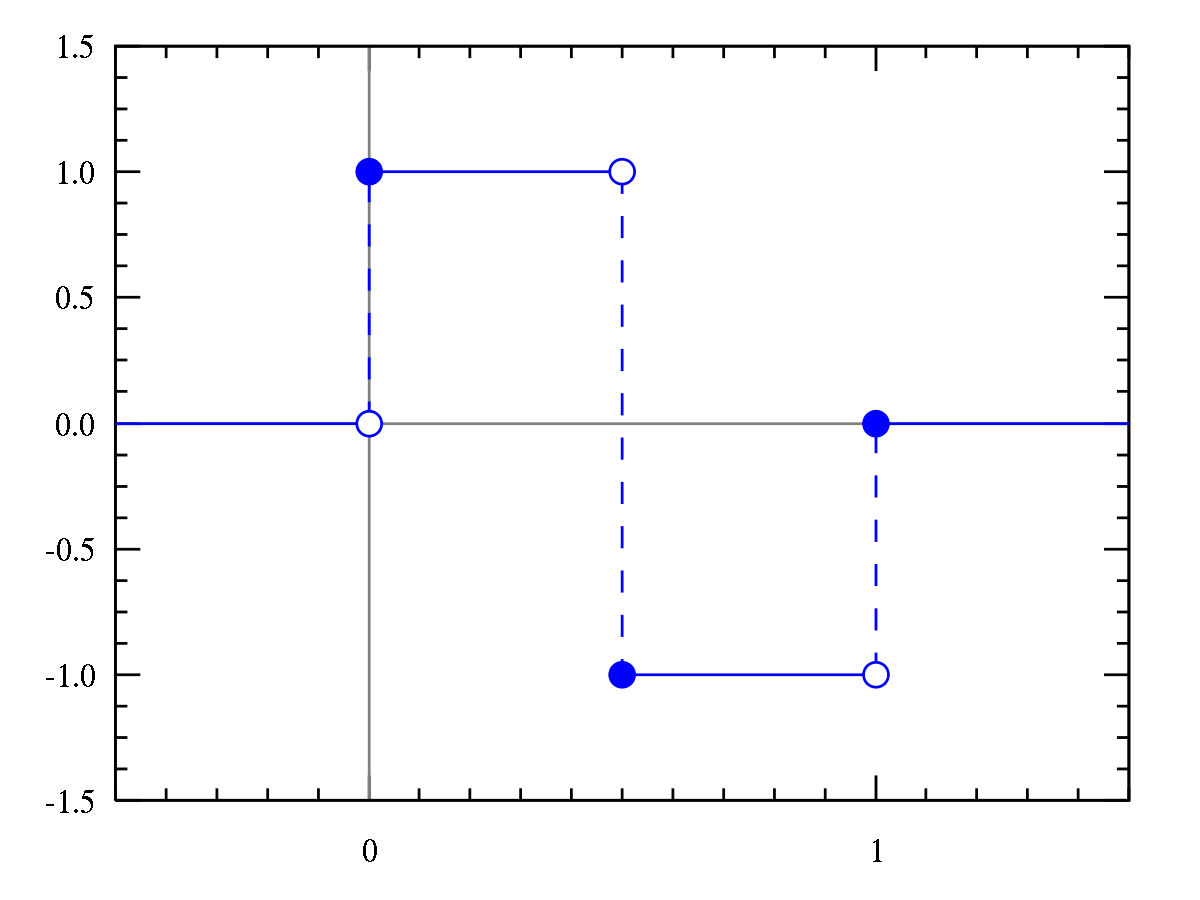
\includegraphics[scale = 0.2]{haar.png}    
	\caption{\gr Κυματίδια \en Haar \protect\url{en.wikipedia.org} \gr}
\end{figure}
Τα κυματίδια \en Haar \gr αποτελούν την πιο απλή μορφή κυματιδίων. Έχουν το εξής ελάττωμα: δεν είναι συνεχή και επομένως δεν είναι παραγωγίσημα. Για τα διακριτά σήματα, όμως, αυτό μπορεί να αποτελέσει πλεονέκτημα. Από την άλλη, ένα πλεονέκτημά τους είναι η ολοκλήρωσή τους λόγω της γραμμικότητάς τους. Ένα ακόμα χαρακτηριστικό τους είναι το εύρος των τιμών που λαμβάνουν, το οποίο αντιστοιχεί σε μόλις 3 αριθμούς: 0, 1, -1. 
\par
Οι τιμές που λαμβάνουν οι συναρτήσεις των κυματιδίων δίνονται από την παρακάτω ακολουθία για το διάστημα 0, 1:
\begin{equation}
	h_i (x) = \begin{cases}
		\text{ 1,  για } x \in [\xi 1, \xi2), \\
		\text{-1, για } x \in [\xi 2, \xi 3), \\
		\text{ 0, αλλιώς}
	\end{cases}
\end{equation}
όπου $\xi 1 = \frac{k}{m}, \xi 2 = \frac{k + 0.5}{m}, \xi 3 = \frac{k + 1}{m}$.
\par\par
Η παράμετρος $m = 2^j, j = 0, 1, ..., J$ δηλώνει το επίπεδο του κυματίου και το $k = 0, 1, ..., m-1$ την παράμετρο μετάφρασης. Ο δείκτης $i$ δίνεται από τη σχέση $i = m + k - 1$. Οι ελάχιστές τιμές είναι  $m = 1, k = 0 $ που δίνουν $i = 2$ και η μέγιστη τιμή του δείκτη είναι $i = 2M = 2J + 1$. [46]-[53]
\par
Αποτελέσματα της χρήσης των κυματιδίων \en Haar \gr στην επεξεργασία σημάτων φαίνεται στην ακόλoυθη εικόνα. Στα αριστερά φαίνεται μια διακριτή χρονοσειρά και στα αριστερά η προσέγγισή της με κυματίδια \en Haar \gr:
\begin{figure}[h!]
	\centering
	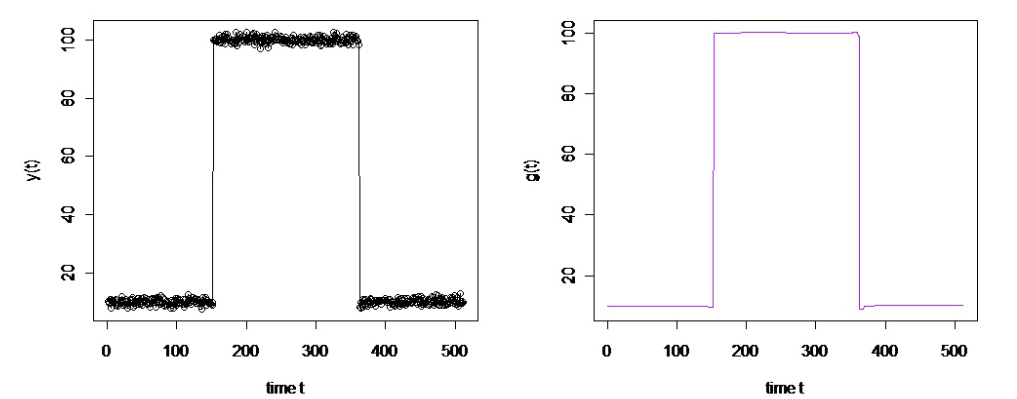
\includegraphics[scale = 0.4]{haar2.png}    
	\caption{\gr Εφαρμογή κυματιδίων \en Haar \gr για συλλογή πληροφοριών από σήμα \en\protect\url{commons.wikimedia.org}}
\end{figure}
\subsection{Μη γραμμικές μέθοδοι}
Σε αυτή την κατηγορία η σχέση των μεταβλητών δεν απεικονίζεται γραμμικά, δηλαδή σε μια ευθεία γραμμή. Οι μη γραμμικές μέθοδοι συνδέονται με την πολυπλοκότητα και την προβλεψιμότητα του σήματος (χρονοσειρά). Οι μη γραμμικές μέθοδοι μας επιτρέπουν να υπολογίσουμε ποσοτικά τη μη προβλεψιμότητα των χρονοσειρών, που πηγάζει από την πολυπλοκότητα των μηχανισμών που ρυθμίζουν το  \en HRV \gr. Για την παρουσίαση των δεδομένων των μη γραμμικών μεθόδων χρησιμοποιείται κυρίως η αναπαράσταση του \en Poincare, \gr η οποία απεικονίζει τη συσχέτιση ανάμεσα σε διαδοχικά \en RR \gr διαστήματα. Οι μέθοδοι αυτές απεικονίζονται με τη βοήθεια της αναπαράστασης του \en Poincare \gr, η οποία αποτελεί ένα χάρτη σημείων στο σύστημα των καρτεσιανών συντεταγμένων φτιαγμένο από τις τιμές των \en RR \gr
διαστημάτων. Αυτή η αναπαράσταση βοηθά στο να εξηγηθούν οι παρακάτω μετρήσεις:\begin{itemize}
	\item \en S: \gr Το εμβαδό της έλλειψης που αντιστοιχεί στο ολικό \en HRV. \gr
	\item \en SD1: \gr Η τυπική απόκλιση (εξ ου και το \en SD \gr) της απόστασης κάθε σημείου από τον άξονα $y=x$, καταδεικνύει το πλάτος της έλλειψης.
	\item \en SD2: \gr Η τυπική απόκλιση της απόστασης κάθε σημείου από τον άξονα $y=x +$ το μέσο \en RR \gr διάστημα, καταδεικνύει το μήκος της έλλειψης. 
	\item \en SD1/SD2: \gr Μετρά τη μη προβλεψιμότητα των \en RR \gr διαστημάτων και συσχετίζεται με το λόγο \en LF/HF. \gr
	\item \en ApEn: Approximate Entropy\gr , μετρά την κανονικότητα και την πολυπλοκότητα μιας χρονοσειράς. Υψηλές τιμές δείχμουν χαμηλή προβλειμότητα της διακύμανσης σε διαδοχικά \en RR \gr διαστήματα.
	\item \en SampEn: Sample Entropy \gr, μετρά την κανονικότητα και την πολυπλοκότητα μιας χρονοσειράς. Σχεδιάστηκε για πιο έμπιστες μετρήσεις και μπορεί να υπολογιστεί σε μικρότερες χρονοσειρές από την \en ApEn \gr.
	\item \en DFA \gr α1: \en Detrended Fluctuation Analysis,\gr υπολογίζει συσχέτιση διαδοχικών RR διαστημάτων. Η κλίση α1 περιγράφει σύντομες εναλλαγές.
	\item \en DFA \gr α2: Η κλίση α2 περιγράφει εναλλαγές μεγαλύτερης διάρκειας από την α1. 
	\item \en D2: \gr Εκτιμά τον ελάχιστο αριθμό μεταβλητών που χρειάζονται για να κατασκευαστεί ένα μοντέλο δυναμικού συστήματος \en (system dynamics, \gr μοντελοποίηση που βοηθά στην κατανόηση μη γραμμικής συμπεριφοράς).
\end{itemize}[44].
\section{Μέθοδοι εκτίμησης μεταβλητότητας καρδιακού ρυθμού}
\subsection{Εντροπία και μέθοδοι εκτίμησης}
Η έννοια της εντροπίας βρίσκει εφαρμογή σε ποικίλους επιστημονικούς κλάδους, κάποιες φορές με πιο αυστηρούς μαθηματικούς ορισμούς και άλλοτε πιο αφηρημένα. Χρησιμοποιείται ευρέως στη φυσική, την κβανοτμηχανική και τη θεωρία πληροφορίας με την επεξεργασία χρονοσειρών. Χρησιμοποιήθηκε και ορίστηκε πρώτη φορά στην εισαγωγή των θερμοδυναμικών συστημάτων (μακροσκοπικός κόσμος) με τον \en Clausius, \gr όταν έθεσε τις πρώτες βασικές έννοιες της εντροπίας στο πλαίσιο της θερμοδυναμικής. Η επιλογή της λέξης «εντροπία» ήταν σκόπιμη, για να τονιστεί η άμεση σύνδεση της εντροπίας με την ενέργεια. Πιο στοχευμένα, όμως, στην παρούσα διπλωματική εργασία οι μέθοδοι εκτίμησης της εντροπίας αντιστοιχούν στους παρακάτω ορισμούς: 
\begin{itemize}
	\item \en Shannon: \gr Στη θεωρία πληροφορίας, ο \en Shannon \gr  όρισε την εντροπία ως έναν τρόπο μέτρησης της αβεβαιότητας της πληροφορίας μιας γραμματοσειράς, χρησιμοποιώντας την στο σύστημα επικοινωνίας. Το σύστημα αυτό αποτελείται από έναν πομπό, ένα δίαυλο μέσω του οποίου εκπέμπεται ένα κωδικοποιημένο σήμα και έναν παραλήπτη, ο οποίος αποκωδικοποιεί το σήμα. Ο \en Shannon \gr όρισε δύο κύριες έννοιές της θεωρίας πληροφορίας: την ποσότητα πληροφορίας και την ομώνυμη εντροπία πληροφορίας. Η ποσότητα πληροφορίας ορίζεται ως:
	\begin{equation}
		I = K ln (M)
	\end{equation}
	με Ι τη συνολική πληροφορία του μηνύματος (συμβολοσειρά), Κ μια σταθερά που επιτρέπει την αλλαγή βάσης του λογαρίθμου, που ισοδυναμεί με την αλλαγή της μονάδας αναπαράστασης της πληροφορίας (π.χ. \en bits \gr). Αν επιλεχθεί το σωστό Κ είναι δυνατή η χρήση οποιασδήποτε λογαριθμικής βάσης. Τέλος, Μ είναι ο συνολικός αριθμός των πιθανών μηνυμάτων ενός πεπερασμένου συνόλου. [59]
	\item \en Rényi: \gr Αυτή η εντροπία αποτελεί γενίκευση της προηγούμενης και όπως η εντροπία του \en Shannon, \gr χρησιμοποιείται και αυτή για τη μέτρηση αβεβαιότητας ενός σήματος. Σε αυτή την περίπτωση υπάρχει η προσθήκη μιας παραμέτρου $\alpha$ (τάξη) που απεικονίζει συχνά ή και σπάνια φαινόμενα. Τα διαφορετικά φαινόμενα αντιστοιχούν σε διαφορετικές τιμές της παραμέτρου και του τύπου εντροπίας. Ο γενικός τύπος του \en Renyi \gr τάξης $\alpha$, \gr με $\alpha \geq 0$ και $\alpha \neq 1$
	\begin{equation}
		H_\alpha (X) = \frac{1}{1 - \alpha} log_2 (\sum_{i=1}^{n}{p_i^\alpha})
	\end{equation}
	όπου η μεταβλητή Χ είναι διακριτή και τυχαία. Η ποσότητα \en $H_\alpha (X)$ \gr είναι μέτρο της εντροπίας της κατανομής $ X = (x_1, ..., x_n)$, μονότονη και μη φθίνουσα συνάρτηση του $\alpha$. Οι ποσότητες $p_i$ είναι οι αντίστοιχες πιθανότητες εμφάνισης.
	\par
	Οι πιο συνηθισμένες τιμές της παραμέτρου είναι οι:
	\begin{itemize}
		\item $\alpha = 1$: Όταν το $\alpha$ συγκλίνει προς το 1, τότε λαμβάνουμε την εντροπία του \en Shannon: \gr
		\begin{equation}
			H_1 (X) = \lim_{\alpha \to 1}
		\end{equation}
		\begin{equation}
			H_\alpha (X) = - \sum_{i=1}^{n}{p_i} log (p_i)
		\end{equation}
		
		\item $\alpha = 2$: Εντροπία του \en Rényi. \gr Όταν η τιμή της τάξης δεν προσδιορίζεται, ως βάση θεωρείται ο αριθμός 2. Αυτή η περίπτωση ονομάζεται επίσης εντροπία σύγκρουσης, και οι μεταβλητές Χ, Υ θεωρούνται ανεξάρτητες.
		\begin{equation}
			H_2 (X) = - log\sum_{i=1}^{n}{p_i^2} = log P(X = Y)
		\end{equation}
		
		\item $\alpha = 0$: Μέγιστη εντροπία. Υποθέτεται πως όλες οι πιθανότητες είναι θετικές και τότε ως εντροπία ορίζεται ο λογάριθμος του πλήθους των τιμών που μπορεί να λάβει το Χ.
		\begin{equation}
			H_0 (X) = log n = log |X|
		\end{equation}
		
		\item $\alpha = \infty$: Ελάχιστη εντροπία και ελάχιστη τιμή της εντροπίας του \en Rényi. \gr και το αποτέλεσμα συγκλίνει στον αρνητικό λογάριθμο της μέγιστης πιθανότητας.
	\end{itemize}
	
	Οι μέχρι στιγμής ορισμοί και μέθοδοι εντροπίας αφορούν μόνο στο φυσικό κόσμο και τις διαστάσεις του. Η ευρέως χρησιμοποιούμενη εντροπία του \en  Shannon \gr δεν εμβαθύνει σε χώρους μεγαλύτερης διάστασης, κάτι πολύ χρήσιμο σε διαφορετικούς κλάδους, όπως η Ιατρική Πληροφορική. Η μελέτη  του καρδιακού παλμού και του \en HRV \gr κάνει αναγκαία την εύρεση μεθόδων που εμβαθύνουν στον \en m\gr-διάστατο χώρο. Στη συνέχεια παραθέτονται και αναλύονται κάποιες από αυτές τις βασικές μεθόδους εκτίμησης της εντροπίας σε αυτόν. [54]-[58]
\end{itemize}
\subsection{Εκτίμηση εντροπίας στο \en m-\gr διάστατο χώρο}
Για λόγους πρακτικότητας θα αποφευχθεί η αναλυτική παρουσίαση των μεθόδων που δε χρησιμοποιήθηκαν σε αυτή τη διπλωματική. Θα παρουσιαστούν, θα εξηγηθούν αλλά δε θα αναλυθούν στον ίδιο βαθμό με αυτές που χρησιμοποιήθηκαν. Ο λόγος που δε χρησιμοποιήθηκαν όλες οι παρακάτω μέθοδοι είναι ότι δεν είναι όλες εφαρμόσιμες στο χώρο ανάλυσης καρδιακών σημάτων. 
\subsubsection{ \en Permutation Entropy \gr ή Εντροπία αντιμετάθεσης}
Aποτελεί μέτρο εκτίμησης πολυπλοκότητας μιας χρονοσειράς. Είναι ένας απλός, υπολογιστικά φθηνός αλγόριθμος που μπορεί να εφαρμοστεί σε σήματα μικρού μήκους. Επιπλέον, λαμβάνει υπόψη τη χρονική σειρά των τιμών στο σήμα, σε αντίθεση με την εντροπία του \en Shannon, \gr επομένως στην \en Permutation Entropy \gr οι δύο χρονοσειρές $X_1 = \{1, 0, 1, 0\}$ και $X_2 = \{1, 0, 0, 1\}$ δε θα δίνουν το ίδιο αποτέλεσμα [60]. 
\par
\begin{figure}[!ht]
	\centering
	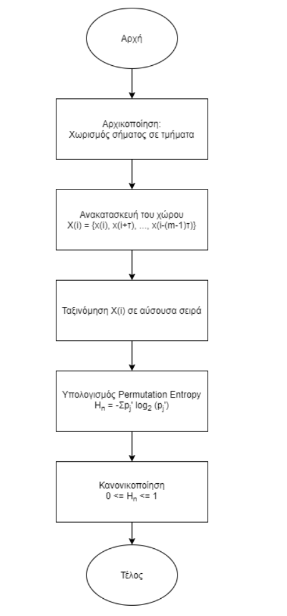
\includegraphics{Permutation.png}    \caption{Βήματα αλγορίθμου της \en Permutation Entropy\gr }
\end{figure}
\par
Τα βήματα του αλγορίθμου παρουσιάζονται επιγραμματικά στο ακόλουθο σχεδιάγραμμα (Σχήμα 3.3). 

\subsubsection{ \en Approximate Entropy (ApEn) \gr}
Ορίστηκε πρώτη φορά το 1995, από τον \en Steve Pincus,\gr  αποτελεί αλγόριθμο εκτίμησης της πολυπλοκότητας μιας χρονοσειράς και. Βασιζόμενη στη Θεωρία Πληροφορίας, εφαρμόζεται σε πολλούς τομείς, μερικοί από τους οποίους είναι η ιατρική, η φυσιολογία, οι τηλεπικονωνίες αλλά και η οικονομία. Η πηγή η οποία παράγει τα δεδομένα δεν επηρεάζει την εφαρμογή της μεθόδου (εφαρμόζεται ανεξάρτητα από αυτή), κάτι που συμβάλλει στην επιτυχία της. Διαθέτει ανθεκτικότητα σε στοχαστικές συμπεριφορές, όπως παρουσία θορύβου. \en H ApEn \gr μελετά την πιθανότητα όμοια μοτίβα σε μια χρονοσειρά να προηγούνται άλλων πρόσθετων όμοιων δεδομένων. Η πιθανότητα επανάληψης είναι αντιστρόφως ανάλογη των τιμών που λαμβάνει, (δηλαδή μικρότερες τιμές αντιστοιχούν σε υψηλή πιθανότητα επανάληψης και αντίστροφα)ς. Οι τρεις βασικές παράμετροι του αλγόριθμου είναι το Ν (το συνολικό μέγεθος των δεδομένων), το \en m \gr (η διάσταση ενσωμάτωσης) και το \en r, \gr η παράμετρος κλίμακας (φίλτρο θορύβου). 
\par
Τα βήματα του αλγορίθμου είναι τα ακόλουθα:
\par
Βήμα 1ο: Έστω η σειρά δεδομένων $u(1), u(2), ..., u(N)$.
\par
Βήμα 2ο: Δίνονται μη αρνητικές τιμές στις παραμέτρους, με $m \leq N$. 
\par
Βήμα 3ο: Ορισμός μιας ακολουθίας διανυσμάτων $x(1), x(2), ..., x(N-m+1)$ στο \en m-\gr διάστατο χώρο $\Re^m$. Τα διανύσματα ορίζονται ως: $x(i) = [u(i), u(i+1), ..., u(i+m-1)]$. Σε αντίθεση με τις προηγούμενες μεθόδους, σε αυτή τη μέθοδο γίνεται χρήση των τιμών του διανύσματος αντί των πιθανοτήτων τους. 
\par
Βήμα 4ο: Για κάθε $i$ στο διάστημα $[1, N-m+1]$, κατασκευάζεται η ακόλουθη ποσότητα με χρήση των διανυσμάτων.
\begin{equation}
	C_i^m (r) = \frac{ \gr \text{πλήθος } x(j) \text{τέτοια ώστε } \en d[x(i), x(j)] \leq r}{N-m+1}
\end{equation}
Όπου $d[x, x*] = max_a |u(a) - u*(a)|$, με $u(a)$ τα βαθμωτά μεγέθη του $x$ και $d$ η μέγιστη απόσταση μεταξύ τους. Τονίζεται πως το $j$ παίρνει όλες τις τιμές, για να συμπεριληφθεί και η ισότητα $j = i$ 
\par 
Βήμα 5ο: Ορίζεται το μέγεθος 
\begin{equation}
	\Phi^m (r) = (N-m+1)^-1 \sum_{i=1}^{N-m+1} log(C_i ^m (r))
\end{equation}
\par
Βήμα 6ο: Ορισμός της \en ApEn \gr ως:
\begin{equation}
	ApEn = \Phi^m (r) - \Phi^m+1 (r)
\end{equation}
με $log$ το φυσικό λογάριθμο για τις τιμές των $m, r$ από το 2ο βήμα.
\par 
Χαμηλές τιμές στον αλγόριθμο υποδεικνύουν ότι το υπό μελέτη σύστημα παρουσιάζει σταθερότητα, μεγάλο βαθμό επανάληψης και δεν περιέχει απρόβλεπτα μοτίβα. Το αντίθετο (υψηλές τιμές) δείχνει ανεξαρτησία ανάμεσα στα δεδομένα και μεγάλο βαθμό τυχαιότητας. Η μέγιστη τιμή που μπορεί να λάβει η \en ApEn \gr σε ένα δυαδικό σύστημα είναι $log2$ (απολύτως τυχαία δεδομένα) και τιμές μικρότερες από αυτή προβλέπουν την ύπαρξη επαναλαμβανόμενων μοντέλων. Όπως προαναφέρθηκε, είναι ανθεκτική σε διάφορες μορφές θορύβου, καθώς τιμές που αποκλίνουν πολύ σε σχέση με τις υπόλοιπες συμβάλλουν σε μικρότερο βαθμό στο συνολικό αποτέλεσμα. Λόγω της κατασκευής του αλγορίθμου και των ριζών του στη Θεωρία Πληροφορίας, η τιμή της είναι μη αρνητική και λαμβάνει την τιμή 0 για τέλειες κανονικές σειρές δεδομένων.
\par
Στον αρχικό ορισμό της \en ApEn \gr η διατήρηση της τάξης δεν είναι απόλυτη, διότι με διαφορετικούς  συνδυασμούς των παραμέτρων $ m, r$ τα αποτελέσματά της διακυμαίνονται σημαντικά. Το βασικό χαρακτηριστικό της χρησιμότητάς της είναι ότι ο βαθμός επαναληψιμότητας, δηλαδή η τυχαιότητα των δεδομένων, αρκεί για το διαχωρισμό των διάφορων συστημάτων. Τα αποτελέσματα, παρόλα αυτά, δεν είναι απόλυτα,καθώς υπάρχουν ζέυγη τιμών που δε διατηρούν αυτή την ιδιότητα. Ο \en Pincus \gr πρότεινε κάποιες προτιμώμενες τιμές σχετικά με τις παραμέτρους $m, r$. Το $m$ προτείνεται να λαμβάνει τις τιμές 2, 3 ενώ το $r$ ανήκει στο διάστημα $[0.1,0.25] std(x)$, με $std(x)$ η τυπική απόκλιση του σήματος. Δεν εφαρμόζονται, όμως, παντού μιας και διαφορετικοί τύποι δεδομένων αντιμετωπίζονται με διαφορετικό τρόπο. Βασικό ερώτημα είναι η τιμή του $r$ που πρέπει να χρησιμοποιείται σε συγκρίσεις μεταξύ διαφορετικών χρονοσειρών.
\par
Αν ισχύει $ApEn(m1, r1)(A)$ τότε ισχύει και $ApEn(m2, r2)(B)$, για κάθε ζεύγος $r2 \geq r1$. Οι προτεινόμενες τιμές ισχύουν για δεδομένα σχετικά με καρδιακό παλμό και έκκριση ορμονών αλλά όχι για δεδομένα νευρικών ώσεων. Οι μεγαλύτερη εφικτή διαφορά στη σύγκριση αποτελεσμάτων ανάμεσα στις τιμές $m, m+1$ δίνεται όταν βρεθεί η τιμή $r$ που μεγιστοποιεί την \en ApEn \gr. Η τιμή $rmax$ είναι αντιστρόφως ανάλογη του μεγέθους των δεδομένων, δηλαδή όσο η τιμή αυξάνεται τόσο μικρότερο είναι το μέγεθος των δεδομένων. Υπό αυτές τις προϋποθέσεις η τιμή ξεφεύγει πολλές φορές από τα συνιστάμενα όρια. Η \en ApEn \gr διαπιστώθηκε πως μπορεί να διαχωρίσει δεδομένα με προσθήκη θορύβου και χαοτικά δεδομένα με σχετικά μικρό αριθμό σημείων (π.χ. 1000) αλλά μπορεί επίσης να εφαρμοστεί με δεδομένα μήκους 100 σημείων αναφοράς, γεγονός πολύ σημαντικό για ανάλυση βιολογικών δεδομένων και ειδικά σε περιπτώσεις που εξετάζονται ασθενείς μεγαλύτερης ηλικίας (Σχήμα 3.4).
\par
Ένας τρόπος για να γίνει πιο κατανοητός ο τρόπος με τον οποίο λειτουργεί η \en ApEn \gr είναι ένα παράδειγμα. Έστω, λοιπόν, $ N = 50$ το μήκος των δεδομένων και η ακολουθία $Χ$ περιέχει τα ακόλουθα 50 δείγματα:
\begin{equation}
	S_N = {61, 62, 63, 64, 65, 61, 62, 63, 64, 65, 61, .., 65}
\end{equation}
(περιοδικά δεδομένα με περίοδο Τ = 5). 
\par
Για λόγους απλότητας ως τιμή του $m$ επιλέγεται το 5 και του $r$ το 2 (αυτές οι τιμές διευκολύνουν τους υπολογισμούς). Αυτό δίνει τα τμήματα:
\begin{equation}
	p_5 (1) = {61, 62, 63, 64, 65}
\end{equation}
\begin{equation}
	p_5 (2) = {62, 63, 64, 65, 61}
\end{equation}
\begin{equation}
	p_5 (3) = {63, 64, 65, 61, 62}
\end{equation}
Αφού η τιμή του $r$ είναι 2 ως κριτήριο ομοιότητας, καθένα από τα 5 στοιχεία του $p_5(i)$ πρέπει να διαφέρουν κατά 2 μονάδες από τα αντίστοιχα του $p_5(1)$. Για αυτό, παραδείγματος χάριν, το $p_5(2)$ δεν είναι όμοιο με το $p_5(1)$ γιατί τα τελευταία στοιχεία τους (61 και 65) διαφέρουν παραπάνω από 2 μονάδες. Τα δεδομένα όμοια του $p_5(1)$ θα είναι τα $p_5(6), p_5(11), . . . , p_5(46)$ (αυτά δηλαδή που διαφέρουν κατά Τ = 5) αλλά και το ίδιο το $p_5(1)$. Αφού το $ N - m + 1 = 50 - 5 + 1 = 46$ και τα στοιχεία που πληρούν τις προϋποθέσεις της απόστασης είναι 10,
\begin{equation}
	C_1,5 (2) = \frac{10}{46}
\end{equation}
Επαναληπτικά, τα $p_5(i)$ όμοια με τα $p_5(2), p_5(3)$ είναι 9. Έτσι, ο μέσος όρος και των 46 $C_i,5 (2)$ είναι:
\begin{equation}
	C_5 (2) = \frac{10\frac{10}{46} + 36\frac{9}{46}}{46} = \frac{424}{2116} \approx 0.200378
\end{equation}
Για να ληφθεί η τιμή της $ApEn(X, 5, 2)$ η παραπάνω διαδικασία πρέπει να επαναληφθεί για $m = 6$. Τα αποτελέσματα, εν συντομία, είναι
\begin{equation}
	n_1,6 (2) = 9
\end{equation}
\begin{equation}
	n_2,6 (2) = 9
\end{equation}
\begin{equation}
	n_3,6 (2) = 9
\end{equation}
\begin{equation}
	...
\end{equation}
\begin{equation}
	C_i,6 (2) = \frac{9}{45} = 0.2, i \leq i \geq 45
\end{equation}
Και $C_6 (2) = 0.2$. To Τελικό αποτέλεσμα είναι 
\begin{equation}
	ApEn(X, 5, 20 = ln[\frac{C_5 (2)}{C_6 (2)}] \approx 0.00189
\end{equation}
Η τιμή αυτή είναι αρκετά μικρή, και υπονοεί πως τα δεδομένα είναι εξαιρετικά προβλέψιμα.
\par
Η $ApEn$, έχει υποβληθεί σε εξονυχιστικούς ελέγχους, παρουσιάζοντας κάποιους περιορισμούς. Κατά το τέταρτο βήμα του αλγόριθμου, υπολογίζεται η ομοιότητα $j = i$ για αποφυγή εμφάνισης του $ln 0$ στους υπολογισμούς. Όλοι οι όροι $C_i ^m (r)$ παραμένουν θετικοί και αν Β θεωρηθούν όλα τα πιθανά διανύσματα και Α όλες οι μετρήσεις ομοιότητας \en (matches) \gr, ο αλγόριθμος υπολογίζει $\frac{A+1}{B+1}$ , που είναι μεγαλύτερο από την κανονική μέτρηση, $\frac{A}{B}$ χωρίς την προσμέτρηση του ίδιου του διανύσματος. Όσο μικρότερο είναι το Ν, τόσο πιο έντονη είναι η διαφορά. Αυτό δημιουργεί απόκλιση της $ApEn$ και οδηγεί σε δύο αρνητικές ιδιότητές της:
\par
Πρώτον, η $ApEn$ εξαρτάται σε μεγάλο βαθμό από το Ν και συχνά σε δεδομένα μικρού μήκους παρουσιάζει μικρότερες τιμές από τις αναμενόμενες.
\par
Δεύτερον, παρουσιάζει έλλειψη συνέπειας. Αν, δηλαδή, η τιμή της για κάποιο σύνολο είναι υψηλότερη από την τιμή κάποιου άλλου συνόλου, θα έπρεπε να παραμένει υψηλότερη για όλες τις εξεταζόμενες συνθήκες (εξαρτάται από τις τιμές του $r$), κάτι που δε συμβαίνει. Η προσθήκη λευκού θορύβου, παραδείγματος χάριν, μπορεί να παρουσιάσει μικρότερες τιμές από κάποιο γνωστό περιοδικό σήμα αν μια από τις παραμέτρους $m, r$ λάβει πολύ μικρές τιμές. Αυτό οδηγεί σε ένα \en “flip” \gr, με αποτέλεσμα ο λευκός θόρυβος να λάβει μεγαλύτερες τιμές όσο οι παράμετροι αλλάζουν τιμή [61]-[67].
\begin{figure}[H]
	\centering
	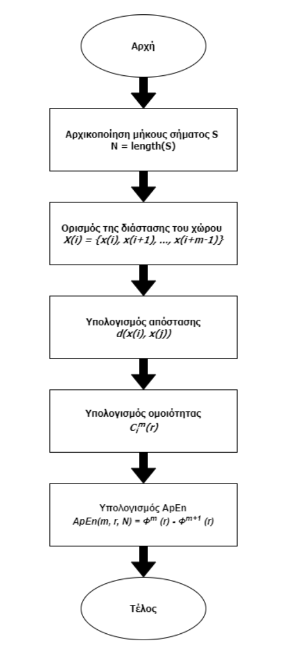
\includegraphics{ApEn.png}    
	\caption{Βήματα αλγορίθμου της \en Approximate Entropy \gr }
\end{figure}

\subsubsection{ \en Sample Entropy \gr}
Οι \en Richman \& Moorman \gr πρότειναν το 2000 τη \en Sample Entropy \gr ως έναν αλγόριθμο με δυνατότητα κάλυψης των αδυναμιών της \en Approximate Entropy. \gr Εξαρτάται και αυτή από τις ίδιες τρεις παραμέτρους και ορίζεται ως ο αρνητικός λογάριθμος της πιθανότητας: αν δύο σύνολα διάστασης $m$ έχουν απόσταση $\leq r$, τότε δύο σύνολα διάστασης $m + 1$, θα έχουν επίσης διαφορά $\leq r$. Συμβολίζεται με $SampEn(m, r, N)$ ή $SampEn(m, r, τ , N)$ αν ληφθεί υπόψιν ο χρόνος δειγματοληψίας $\tau$ . Ο αλγόριθμος αρχίζει να φιαφέρει από αυτόν της $ApEn$ από το σημείο ορισμού των $C_i ^ m (r)$ και μετά, όπου αντικαθίστανται από τα $n_m (r)$ και $n_m+1 (r)$, τις πιθανότητες ένα σημείο να είναι όμοιο με ένα άλλο στις διαστάσεις $m$ και $m+1$ αντίστοιχα:
\begin{equation}
	n_m (r) = \sum_{j=1}{N-m} \Theta (i, j, m, r), i \neq j
\end{equation}
\begin{equation}
	n_m+1 (r) = \sum_{j=1}{N-m} \Theta (i, j, m+1, r), i \neq j
\end{equation}
όπου
\begin{equation}
	\Theta (i, j, m, r) = \begin{cases}
		1, & \text{αν $||x_i - x_j||_m \leq r, j \leq i$}.\\
		0, & \text{αλλιώς}.
	\end{cases}
\end{equation}
Η \en Sample Entropy \gr δίνεται από το λόγο
\begin{equation}
	\begin{aligned}
		SampEn (m, r) = ln \frac{B^m (r)}{A^m (r)} = \lim_{N \to \infty} - \log [\frac{A^m (r)}{B^m (r)}] = \\ 
		\lim_{N \to \infty} - \log [\frac{\frac{1}{N-m} \sum_{i=1}^{N-m} A_i ^m (r)}{\frac{1}{N-m} \sum_{i=1}^{N-m} B_i ^m (r)}]
	\end{aligned}
\end{equation}
Τα $B^m (r)$ είναι η πιθανότητα δυο ακολουθίες να είναι όμοιες στη διάσταση $m$ και τα $A_m(r)$ είναι η πιθανότητα δύο ακολουθίες να είναι όμοιες στη διάσταση $m + 1$ και αποτελούν το μέσο όρο των αθροισμάτων των όρων $B_i ^m (r)$ και $Α_i ^m (r)$ που μετρούν την ομοιότητα των όρων στις αντίστοιχες διαστάσεις.
\begin{equation}
	B_i ^m (r) = \frac{1}{N - m + 1} n_m , i = 1, ..., N - m
\end{equation}
\begin{equation}
	A_i ^m (r) = \frac{1}{N - m + 1} n_m+1 , i = 1, ..., N - m
\end{equation}
Οι $SampEn$ και $ApEn$ έχουν τρεις διαφορές. Πρώτον, η $SampEn$ θεωρείται ανεξάρτητη του
μήκους $Ν$, δε συγκρίνει δηλαδή το διάνυσμα υπό μελέτη με τον εαυτό του. Δεύτερον, το άθροισμα των διανυσμάτων της βρίσκεται εντός του λογαρίθμου, ενώ στην $ApEn$ βρίσκεται εκτός. Η ανισότητα του $Jensen$ λέει ότι $\log (\sum) > \sum \log$ και αυτός ο όρος είναι μεγαλύτερος στη $SampEn$. Τέλος, η $ApEn$ περιέχει τον παράγοντα $\frac{1}{N-m}$, που την κάνει εξαρτώμενη από το $Ν$, σε αντίθεση με την $SampEn$. Ανεξαρτήτως από τις διαφορές τους, τα αποτελέσματα και των δύο εξαρτώνται εξίσου από τις άλλες δύο παραμέτρους $m, r$ και την τιμή που αυτές θα λάβουν. Επιπλέον, στη $SampEn$ όπως και στη $ApEn$, υψηλές τιμές δηλώνουν ανεξάρτητα δεδομένα, χωρίς επαναλήψεις και χαμηλές τιμές δείχνουν επανάληψη και μεγαλύτερη προβλεψιμότητα. Μια γενική σύγκριση των
τύπων παρουσιάζεται εδώ:
\begin{equation}
	\begin{aligned}
		SampEn (m, r, N) = \\
		- \log \frac{\sum_{i=1}^{N-m} \sum_{j=1 , j\neq i}^{N-m} \text{αριθμός φορών που ισχύει } d[| x_m+1 (j) - x_m+1 (i) |] < r}{\sum_{i=1}^{N-m} \sum_{j=1 , j\neq i}^{N-m} \text{αριθμός φορών που ισχύει } d[| x_m (j) - x_m (i) |] < r}
	\end{aligned}
\end{equation}
\par
\begin{equation}
	\begin{aligned}
		ApEn (m, r, N) \simeq - \frac{1}{N-m} \\
		\sum_{i=1}^{N-m} \log \frac{\sum_{j=1}^{N-m} [\text{αριθμός φορών που ισχύει } d[| x_m+1 (j) - x_m+1 (i) |] < r]}{\sum_{j=1}^{N-m} [\text{αριθμός φορών που ισχύει } d[| x_m (j) - x_m (i) |] < r]}
	\end{aligned}
\end{equation}
\par
Ακολουθεί ένα παράδειγμα χρήσης της $SampEn$. Έστω η χρονοσειρά $Ξ(Ν) = {0.1, 0.1, 0.2, 0.5,
	0.22}$ και έστω $m = 2, r = 0.2$ και $ N = 5$. Το μέγεθος του $A^m(r)$ είναι $Ν$ και του $B^m(r) Ν-1$. Άρα οι ακολουθίες για τα $A^m(r)$ και $B^m(r)$, αντίστοιχα, είναι $ \{0.1, 0.1, 0.2, 0.5, 0.22\}$ και $\{0.1, 0.1, 0.2, 0.5\}$. Για $m = 2$ οι πιθανές ακολουθίες είναι $\{(0.1, 0.1, 0.2), (0.1, 0.2, 0.5)\}$, \\
$\{(0.1, 0.1, 0.2), (0.2, 0.5, 0.22)\}, \{(0.1, 0.2, 0.5), (0.2, 0.5, 0.22)\}$. Σύμφωνα με την εξίσωση: 
\begin{equation}
	SampEn (m, r, N) = - \ln{\frac{A}{B}}
\end{equation}
\begin{equation}
	A = \frac{[(n - m - 1)(n - m)]}{2} A^m (r)
\end{equation}
\begin{equation}
	B = \frac{[(n - m - 1)(n - m)]}{2} B^m (r)
\end{equation}
H $SampEn$ υπολογίζεται ως: 
\begin{equation}
	SampEn (0, 0.2, 5) = p(0) = - \ln{\frac{A[0]}{(N * N - 1)/2}} = - \ln{610} = 0.5108
\end{equation}
\begin{equation}
	SampEn (1, 0.2, 5) = p(1) = - \ln{\frac{A[1]}{B[0]}} = - \ln{\frac{1}{3}} = 1.0986
\end{equation}
\begin{equation}
	SampEn (2, 0.2, 5) = p(2) = - \ln{\frac{A[2]}{B[1]}} = - \ln{0} = \infty
\end{equation}
\par
H $SampEn$ χρησιμοποιεί ολοκληρώματα συσχέτισης που ορίζονται στη θεωρία του χάους ως η μέση πιθανότητα δύο καταστάσεων σε δύο διαφορετικές στιγμές να βρίσκονται κοντά η μία στην άλλη.
\begin{equation}
	C(\varepsilon) = \lim_{N \to \infty} \frac{1}{N^2} \sum_{i, j = 1, i \neq j}^{N} \Theta (\varepsilon - || \overrightarrow x (i) - \overrightarrow x (j)||), \overrightarrow x (i)   \epsilon  \Re^m
\end{equation}
$N$ είναι ο αριθμός των υποτιθέμενων καταστάσεων, $\epsilon$ το κατώφλι της απόστασης.
\par
Ακόμη και αν διαφέρουν σε δομή και μαθηματικό υπόβαθρο, το συμπέρασμα είναι πως τόσο
$SampEn$ όσο και η $ApEn$ αποτελούν μεθόδους εκτίμησης πολυπλοκότητας χρονοσειρών και επηρεάζονται εξίσου από την τιμή των παραμέτρων $m, r$, η λάθος επιλογή των οποίων οδηγεί σε ανακριβή αποτελέσματα και για τις δύο. Με την πάροδο του χρόνου άλλες βελτιωμένες μορφές της $SampEn$ έχουν προταθεί [61]-[62], [67]-[69].
\subsubsection{\en Bubble Entropy \gr}
Η \en Bubble Entropy \gr αποτελεί μια νέα μετρική σχετικά με τη μέτρηση της εντροπίας σχετικής με το \en HRV. \gr Η βασική της διαφορά σε σχέση με τις προαναφερθείσες \en ApEn \gr και \en SampEn \gr είναι η μειωμένη της εξάρτηση από τις παραμέτρους $m, r$. Πιο συγκεκριμένα, η εξάρτησή της από την παράμετρο $r$ είναι μηδενική και όσον αφορά τη $m$, η σημαντικότητά της έχει μειωθεί.
\par 
Η απεξάρτηση από την $r$ έγινε εφικτή μέσω της συμβολικής ανάλυσης (Σχήμα 3.5). Στην \en Bubble Entropy \gr το εύρος τιμών της χρονοσειράς χωρίζεται σε διαστήματα που ονομάζονται από κάποια σύμβολα, όπως παραδείγματος χάριν τα γράμματα της αλφαβήτου. Τα στοιχεία λαμβάνουν το όνομά τους από το διάστημα στο οποίο ανήκουν και η αντιστοίχηση αυτή δίνει την τιμή της εντροπίας. Το μέγεθος των λέξεων καθορίζεται από την παράμετρο $m$, που αντιστοιχεί στη διάσταση του χώρου. Η σύνδεση των "ονομάτων" είναι εφικτή μέσω της κατάστασης: πανομοιότυπα/ίδια ή διαφορετικά. 
\par
Το μέγεθος των διαστημάτων κατέληξε να αντικαταστήσει την παράμετρο $r$. Για να αποβληθεί η εξάρτηση, πρέπει ο διαχωρισμός των διαστημάτων να μην είναι καθορισμένος. Το πρόβλημα αυτό λύνεται με την ενσωμάτωση της χρονοσειράς στο $m$-διάστατο χώρο. Μετά από αυτό το βήμα, κάθε διάνυσμα αντιστοιχίζεται σε ένα σημείο στο χώρο ($m$-διάστατο) και τα διαστήματα διαχωρισμού καθορίζονται με βάση τις τιμές του διανύσματος. Κάθε τιμή του διανύσματος λαμβάνει το όνομα του διαστήματος στο οποίο ανήκει, μετατρέποντας το διάνυσμα σε μια λέξη από σύμβολα μήκους $m$.
\begin{figure}[h!]
	\centering
	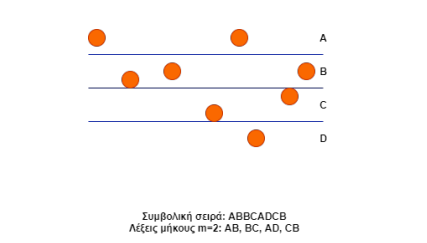
\includegraphics[scale = 0.7]{Bubble.png}    
	\caption{\gr Συμβολική ανάλυση με λέξεις μήκους $m = 2$}
\end{figure}

Όπως μπορεί να παρατηρηθεί, γίνεται κατανοητή η μοναδικότητα της κάθε λέξης, και η μοναδική της εμφάνιση. Επιπλέον, τα σύμβολα που χρησιμοποιούνται για την παραγωγή των λέξεων ανήκουν στο διάστημα [1, $m$] και το κάθε σύμβολο αντιστοιχεί στη θέση που θα είχε το εκάστοτε στοιχείο του διανύσματος αν είχε ταξινομηθεί. H διαδικασία αυτή ορίζει την πολυπλοκότητα στην οποία βασίστηκε ο αλγόριθμος της εν λόγω μετρικής. Ο αλγόριθμος που χρησιμοποιήθηκε είναι ο \en Bubble sort, \gr από τον οποίο προέρχεται και το όνομα της \en Bubble Entropy. \gr Κατά τον υπολογισμό της καταγράφεται ο αριθμός των απαιτούμενων αλλαγών για την ταξινόμηση του κάθε διανύσματος ξεχωριστά. Τα βήματα αυτά εκφράζουν μια πολυπλοκότητα, τα οποία καθιστούν την \en Bubble Entropy \gr μέθοδο εκτίμησης εντροπίας. 
\par
Τα βήματα που ακολουθεί ο αλγόριθμος είναι τα εξής  (Σχήμα 3.6):
\begin{itemize}
	\item Ενσωμάτωση του σήματος στο χώρο διάστασης $m$.
	\item Μέτρηση πλήθους αλλαγών (\en swaps \gr) για την ταξινόμηση του κάθε διανύσματος.
	\item Δημιουργία νέας ακολουθίας με το πλήθος των αλλαγών. 
	\item Εκτίμηση εντροπίας με βάση την εντροπία του \en Renyi \gr για το κάθε διάνυσμα.
	\item Επανάληψη των βημάτων για τη διάσταση $m + 1$. 
\end{itemize}
Μετά τον υπολογισμό των βημάτων, η \en Bubble Entropy \gr λαμβάνει την τιμή της από τη διαφορά εντροπίας ανάμεσα στις διαστάσεις $m$ και $m + 1$.
Όπως και οι δύο προηγούμενες μετρικές, η \en Bubble Entropy \gr υπολογίζει τη διαφορά εντροπίας ανάμεσα στους δύο πολυδιάστατους χώρους που διαφέρουν κατά ένα. Η χρήση της εντροπίας \en Rényi \gr τονίζει τις απότομες αλλαγές που περιέχονται στα σήματα, λόγω της δεύτερης τάξης που περιέχει. 
\par
Τέλος, έχει αποδειχθεί το πλεονέκτημα της ανοχής της σε έντονες κορυφές (\en "spikes"\gr) που περιέχονται σε καρδιακά σήματα κατά την καταγραφή από ΗΚΓ, το οποίο είναι μεγαλύτερο σε σύγκριση με τη \en Sample Entropy, \gr μετά την προσθήκη τεχνητού θορύβου. Στη συνέχεια, καθορίστηκε η τιμή των παραμέτρων και υπολογίστηκε η τιμή λάθους ανάμεσσα στις δύο μεθόδους. Σε κάθε περίπτωση, το λάθος της \en Bubble Entropy \gr ήταν μικρότερο από αυτό της \en Sample Entropy. \gr Οι δυνατότητες της \en Bubble Entropy \gr έχουν αποδειχθεί και σε μια προσπάθεια σύγκρισής της με την \en Permutation Entropy. \gr Οι ερευνητές συνέκριναν τις ομοιότητες και τις διαφορές των δύο μετρικών. Παραδείγματος χάριν, οι ακολουθίες ${2, 4, 6}, {6, 2, 4}$ είναι διαφορετικές για την \en Permutation Entropy \gr αλλά ίδιες για την \en Bubble Entropy \gr μιας και απαιτείται ο ίδιος αριθμός εναλλαγών για την ταξινόμησή τους.

\begin{figure}[!ht]
	\centering
	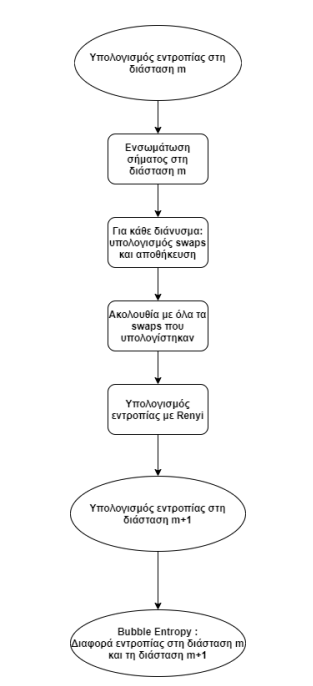
\includegraphics[scale = 0.5]{Bubble2.png}    
	\caption{Τα βήματα του αλγορίθμου της \en Bubble Entropy\gr }
\end{figure}

Πραγματοποιήθηκαν δύο σειρές πειραμάτων· στην πρώτη σειρά ερευνήθηκαν οι μεταξύ τους διαφορές και στη δεύτερη υπολογίστηκε η μεταξύ τους συνέργεια, συνδυάζοντας και τις δύο σε μια σύνθετη μέθοδο ομαδοποίησης, με εύρος διαφορετικών δεδομένων που προήλθαν τόσο από ηλεκτροκαρδιογράφημα όσο και από ηλεκτροεγκεφαλογράφημα, για την εξαγωγή πιο ολοκληρωμένων αποτελεσμάτων. 
\par
Η πρώτη σειρά πειραμάτων έδειξε πως οι δύο μέθοδοι δρούσαν με συμπληρωματικό τρόπο. Το ίδιο αποδείχθηκε και για τα δυνατά σημεία και των δύο μεθόδων. Όσον αφορά στην ακρίβειά τους στα διαφορετικά σήματα, η \en Permutation Entropy \gr έδειξε μια υπεροχή σε αυτά με περισσότερη ομαλότητα, ενώ η \en Bubble Entropy \gr στα σήματα με πιο απότομες διακυμάνσεις. 
\par
Στη δεύτερη σειρά πειραμάτων, τα αποτελέσματα ήταν ανάλογα με
το είδος των εξεταζόμενων σημάτων. Η νέα μέθοδος μπορούσε σε μερικές περιπτώσεις να ομαδοποιήσει τα σήματα πιο αποτελεσματικά από ό,τι η κάθε μέθοδος ξεχωριστά, αν και αυτό δεν υφίστατο σε όλες τις περιπτώσεις. Θεωρήθηκε, λοιπόν, πως αυτή η περίπτωση χρίζει αναλυτικότερης και βαθύτερης μελέτης. 
\par 
Ως τελευταίο παράδειγμα αναφοράς της ικανότητας της \en Bubble Entropy \gr μπορεί να ληφθεί η προσωπική μου προπτυχιακή εργασία επάνω στη μελέτη της ανθεκτικότητάς της σε τεχνητό θόρυβο. Σε αυτή την εργασία δημιουργήθηκαν τεχνητοί έκτοποι παλμοί σε πραγματικά δεδομένα τα οποία λήφθηκαν από τη βάση δεδομένων του \en PhysioNet \gr και μελετήθηκε η ανεκτικότητα της \en Bubble Entropy \gr σε σύγκριση με τις \en Approximate Entropy \gr και \en Sample Entropy \gr στο θόρυβο που προκαλούσαν αυτα τα σήματα. Σχεδόν σε όλες τις σειρές πειραμάτων που δημιουργήθηκαν, η \en Bubble Entropy \gr έδειχνε πολυ ταχύτερη σύγκλιση και σταθερότητα σχετικά με τις άλλες δύο μεθόδους εκτίμησης εντροπίας, γεγονός που ενισχύει τη χρησιμότητά της και τις δυνατότητες που διαθέτει στην εκτίμηση της εντροπίας σε καρδιακά σήματα [69]-[71], [74]. 

\subsubsection{ \en Multiscale Entropy \gr }
Aποτελεί αλγόριθμο εκτίμησης πολυπλοκότητας πεπερασμένων σειρών. Χρησιμοποιείται σε συνδυασμό με τη \en Sample Entropy, \gr η οποία βασίζεται στην εκτίμηση της προβλεψιμότητας της χρονοσειράς, όπως έχει προαναφερθεί. Το κενό αυτό καλύπτει η \en Mutiscale Entropy. \gr Στα δύο στάδια του αλγορίθμου, εφαρμόζεται ένας αδρός διαμοιρασμός στη χρονοσειρά, συχνά παραπάνω από μια φορά (σε κάθε νέα χρονοσειρά, τα σημεία της αποτελούνται από συνδυασμό 2 ή περισσότερων σημείων της προηγούμενης χρονοσειράς).
\par
\begin{figure}[!ht]
	\centering
	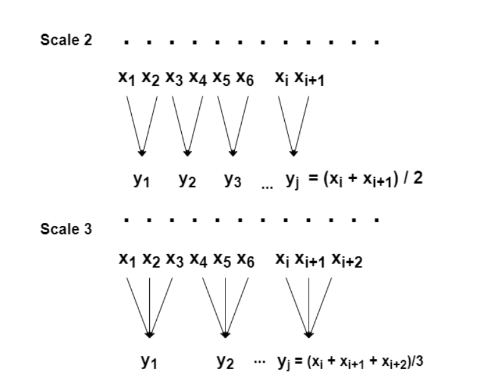
\includegraphics{Multiscale.png}    \caption{Βήματα αλγορίθμου της \en Multiscale Entropy \gr }
\end{figure}
\par
Στο δεύτερο στάδιο, εφαρμόζεται η \en Sample Entropy \gr σε κάθε μία πό τις χρονοσειρές. Η \en Sample Entropy \gr αναζητά επαναλαμβανόμενα μοτίβα σε μια χρονοσειρά και υπολογίζει την προβλεψιμότητα της χρονοσειράς. Ένα πρόβλημα που προκύπτει κατά την εφαρμογή της \en Multiscale Entropy \gr είναι το μέγεθος των δεδομένων. Για να ληφθούν σωστά τα αποτελέσματα χρειάζεται πραγματοποίηση ελέγχου στις μεγαλύτερες χρονικές κλίμακες. Στο αντίστοιχο διάγραμμα εμφανίζονται περιληπτικά τα βήματα του αλγόριθμου της \en Multiscale Entropy (Σχήμα 3.7). [72]-[73] \gr

\newpage
%\iffalse
\documentclass{report}
\usepackage{graphicx} % Required for inserting images
\usepackage[utf8]{inputenc}
\usepackage[main=greek,english]{babel}
\usepackage{longtable}
\usepackage[utf8]{inputenc}
\usepackage{longtable}
\usepackage{tabu}
\usepackage{amsmath}
\usepackage{float}
\usepackage{pdfpages}
\usepackage{subfiles}
\newcommand\tab[1][1cm]{\hspace*{#1}}
\newcommand \en {\selectlanguage{english}}
\newcommand \gr {\selectlanguage{greek}}
\usepackage[euler]{textgreek}
\usepackage{import}
\usepackage{subfig}
\usepackage[a4paper,width=150mm,top=25mm,bottom=25mm]{geometry}
\usepackage{amsmath}
\usepackage{caption}
\usepackage{url}
\usepackage[T1]{fontenc}
\usepackage[pages=some]{background}

\usepackage{fancyhdr}
%\begin{document}
\fi
\gr
\chapter{Πειραματική Ανάλυση}
Η επεξεργασία, η μελέτη των καρδιογραφημάτων αλλά και του \en HRV \gr έχουν συμβάλλει στην πρόληψη της εμφάνισης αρκετών καρδιακών παθήσεων και ασθενειών καθώς και στη διάγνωσή τους. Με την εφαρμογή διαφορετικών μετρικών, αλγορίθμων και μεθόδων η ακρίβεια των αποτελεσμάτων αυξάνεται.
\par
Στο τρέχον κεφάλαιο θα αναλυθούν τα πειράματα που εκπονήθηκαν για αυτή τη διπλωματική εργασία με σκοπό να γίνει πιο ακριβής η πιθανότητα πρόληψης εμφάνισης και διάγνωσης ποικίλων καρδιακών αρρυθμιών. Χρησιμοποιήθηκαν διαφορετικές βιβλιοθήκες που αντιστοιχούν σε μια πληθώρα καρδιακών αρρυθμιών, ώστε να βοηθηθεί η απόδοση του αλγορίθμου σε μεγαλύτερο πλήθος περιπτώσεων. Εφαρμόστηκαν αρκετές από τις μετρικές και μεθόδους που αναλύθηκαν στα προηγούμενα κεφάλαια και η μόνη επεξεργασία που υπέστησαν τα δεδομένα ήταν αυτή που αντιστοιχεί σε φιλτράρισμα για αφαίρεση θορύβου. Κάποια από τα δεδομένα αποκλείστηκαν, όταν μετά τη διεξαγωγή των πειραμάτων κρίθηκαν ακατάλληλα. Σε όλες τις βιβλιοθήκες εφαρμόστηκαν οι ίδιες μετρικές και μέθοδοι και όλα τα γραφήματα απεικονίζονται με τον ίδιο τρόπο για κάθε διαφορετική μετρική και μέθοδο. Σκοπός των πειραμάτων είναι η οδήγηση στη χρήση ενός ενιαίου αλγόριθμου με δυνατότητα εντοπισμού περιοχών που αποκλίνουν από τη φυσιολογική λειτουργία και πιθανώς αποτελούν κίνδυνο για τον ασθενή. 
\par
Στη συνέχεια παραθέτονται αναλυτικότερα τα δεδομένα, ο προσδιορισμός των μετρικών και των μεθόδων και η αξιολόγηση των αποτελεσμάτων. Παραθέτονται επίσης τα γραφήματα που δημιουργήθηκαν ως αποτέλεσμα εκτέλεσης του αλγορίθμου σε όλες τις βιβλιοθήκες. Το κεφάλαιο χωρίζεται σε δύο βασικά μέρη: τη μεθοδολογία και τα αποτελέσματα της πειραματικής ανάλυσης.
\section{Μεθοδολογία}
\subsection{Τα δεδομένα}
Τα δεδομένα που χρησιμοποιήθηκαν ανήκουν εξ ολοκλήρου στη βάση δεδομένων του \en Physionet, \gr η οποία περιέχει σήματα διαφορετικών τύπων όπως εγκεφαλογραφήματα, καρδιογραφήματα, καρδιοτοκογραφήματα. 
Πιο αναλυτικά, έγινε χρήση των παρακάτω βιβλιοθηκών: \en 
\begin{itemize}
	\item Long Term AF Database: \gr αποτελείται από 84 καταγραφές από ασθενείς με παροξυσμική και παρατεταμένη κολπική μαρμαρυγή. Η διάρκεια καταγραφής ποικίλει αλλά κατά μέσο όρο κυμαίνεται ανάμεσα σε 24 και 25 ώρες. Στο Σχήμα 4.1 παρουσιάζεται ενδεικτικά ένα από τα δείγματα της βιβλιοθήκης. Είναι εύκολα αντιληπτό πως τα σήματα περιέχουν μεγάλο ποσοστό θορύβου τόσο από εξωγενείς όσο και από ενδογενείς παράγοντες (παρεμβολή από ηλεκτρόδια, θόρυβος από την κίνηση κατά τη διάρκεια καταγραφής) αλλά επιπλέον τα σήματα δείχνουν πολύ πυκνούς και συνεχόμενα έντονους παλμούς. Επιπλέον, η μεγάλη χρονική διάρκεια συμβάλλει στη δημιουργία πυκνών καταγραφών, κάνοντας μεν την εκτίμηση δυσκολότερη (Σχήμα 4.1).
	\begin{figure}
		\centering
		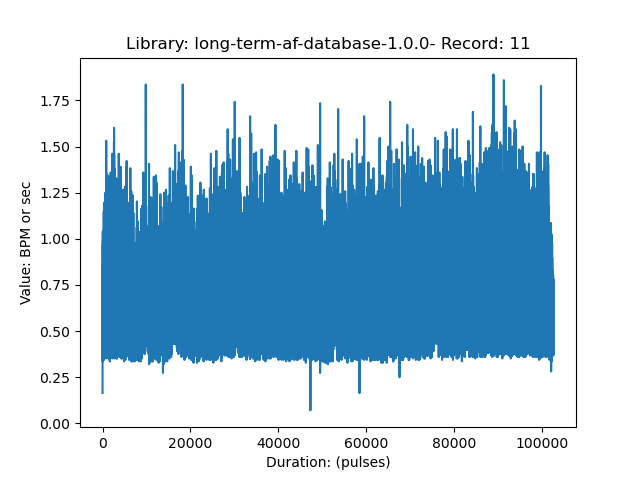
\includegraphics[width=.24\textwidth]{long-term-af-db/long-term-af-database-1.0.0_11.png}
		\caption{\gr Δείγμα βιβλιοθήκης \en Long Term AF Database \gr (αρχικά δείγματα/καταγραφές)}
	\end{figure}
	
	\item \en MIT-BIH Arrhythmia Database: \gr περιέχει 48 καταγραφές που ανήκουν σε 47 ασθενείς, με διάρκεια ελαφρώς μεγαλύτερη της μισής ώρας. Τα σήματα εδώ είναι συντομότερα και ο θόρυβος δε φαίνεται να πυκνώνει ακραία το σήμα. Συγκριτικά, λοιπόν, με την προηγούμενη βιβλιοθήκη παρατηρούνται με μεγαλύτερη ευυκολία περιοχές φυσιολογικής και μη λειτουργίας ακόμα και με το μάτι. Δε γίνεται συγκεκριμένος ο τύπος αρρυθμιών σε αυτή τη συλλογή, άρα γίνεται η υπόθεση πως περιέχει περισσότερες από μία. Η μορφολογία των σημάτων 
	διαφέρει: συμπεριλαμβάνονται τόσο σήματα με έντονο θόρυβο και μόνιμα άστατο καρδιακό ρυθμό, όσο και σήματα με ποικιλομορφίες (φαινομενική ομοιομορφία/ ηρεμία παλμών και ξαφνική απώλεια παλμών ή εμφάνιση πολύ υψηλών αριθμητικά τιμών). Είναι, επομένως, πιο εύκολα ερμηνεύσιμα σε σύγκριση με μερικές από τις υπόλοιπες μελετώμενες βιβλιοθήκες (Σχήμα 4.2). 
	\begin{figure}
		\centering
		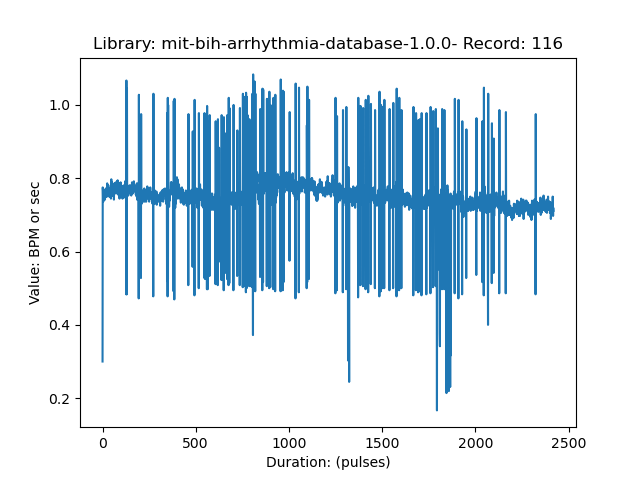
\includegraphics[width=.24\textwidth]{mitbih-arr-db/mit-bih-arrhythmia-database-1.0.0_116.png}
		\caption{\gr Δείγμα βιβλιοθήκης \en MIT-BIH Arrhythmia Database \gr (αρχικά δείγματα/καταγραφές)}
	\end{figure}
	\item \en MIT-BIH Atrial Fibrillation Database: \gr περιλαμβάνει 25 καταγραφές από ασθενείς με (κατά βάση) παροξυσμική κολπική μαρμαρυγή. Η διάρκεια των σημάτων είναι πολύ σύντομη, επομένως η εκτίμηση περιοχών μη φυσιολογικής λειτουργίας παρεμποδίζεται λόγω έλλειψης παρεμφερών δειγμάτων (Σχήμα 4.3).
	\begin{figure}
		\centering
		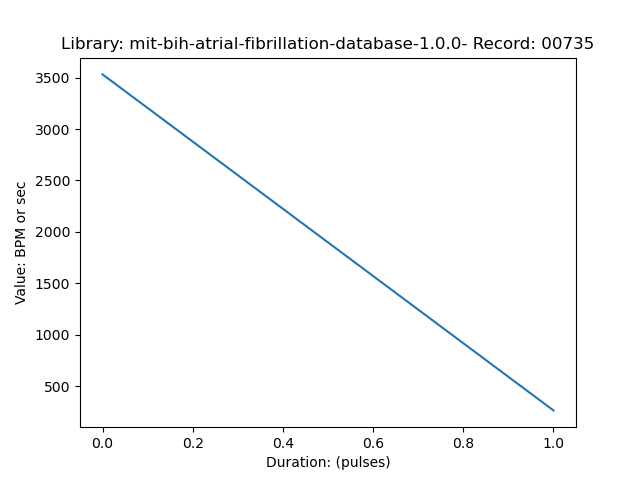
\includegraphics[width=.24\textwidth]{mitbih-af/mit-bih-atrial-fibrillation-database-1.0.0_00735.png}
		\caption{\gr Δείγμα βιβλιοθήκης \en MIT-BIH Atrial Fibrillation Database \gr (αρχικά δείγματα/καταγραφές)}
	\end{figure}
	\item \en MIT-BIH Malignant Ventricular Ectopy Database: \gr αυτή η ομάδα καταγραφών περιέχει κοιλιακές αρρυθμίες (παρατεταμένη κοιλιακή ταχυκαρδία, κοιλιακό πτερυγισμό και κοιλιακή μαρμαρυγή). Οι 22 καταγραφές έχουν διάρκεια μισής ώρας. Παρεμφερής με τη βιβλιοθήκη \en MIT-BIH Atrial Fibrillation Database \gr παρατηρείται η μικρής έκτασης διάρκεια στις καταγραφές και τίθεται το ερώτημα της δυνατότητας εξαγωγής συμπερασμάτων από αυτή τη συλλογή σημάτων (Σχήμα 4.4). 
	\begin{figure}
		\centering
		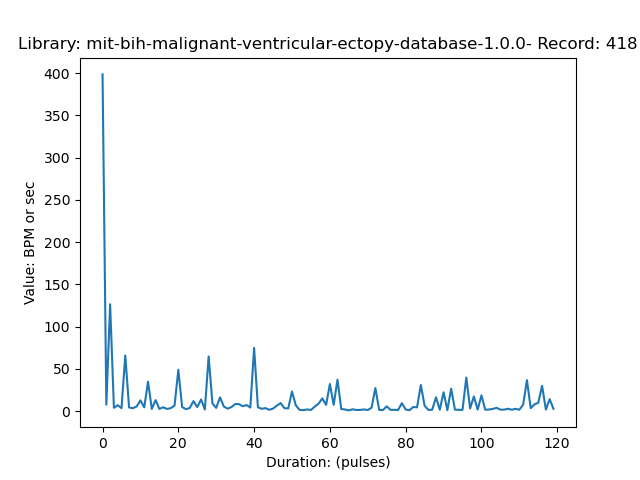
\includegraphics[width=.24\textwidth]{malignant/mit-bih-malignant-ventricular-ectopy-database-1.0.0_418.png}
		\caption{\gr Δείγμα βιβλιοθήκης \en MIT-BIH Malignant Ventricular Ectopy Database \gr (αρχικά δείγματα/καταγραφές)}
	\end{figure}
	\item \en MIT-BIH Supraventricular Arrhythmia Database: \gr αποτελείται από 78 καταγραφές διάρκειας 30 λεπτών (ανάμεσα σε 30 και 40) και οι ασθενείς υπέστησαν επεισόδια υπερκοιλιακών αρρυθμιών. Η τριαντάλεπτη καταγραφή κάνει πιο εύκολη τη διάκριση ανάμεσα σε αποκλίνοντες καρδιακούς παλμούς ακόμα και με το μάτι και διευκολύνει τόσο την ερμηνεία όσο και την αξιολόγηση των δειγμάτων. Όπως και στις υπόλοιπες βιβλιοθήκες, ο έντονος θόρυβος που παρατηρείται \en (spikes) \gr δεν είναι πραγματικοί καρδιακοί παλμοί αλλά θόρυβος που εμφανίζεται κατά την καταγραφή και δημιουργία των ηλεκτροκαρδιογραφημάτων (Σχήμα 4.5).
	\begin{figure}
		\centering
		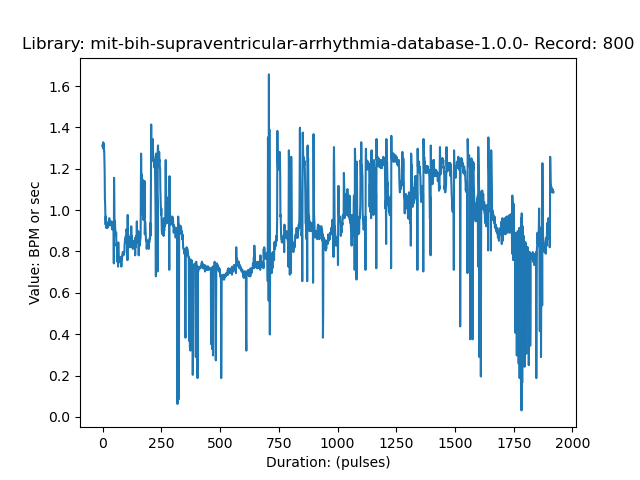
\includegraphics[width=.24\textwidth]{mitbih-supraventricular-db/mit-bih-supraventricular-arrhythmia-database-1.0.0_800.png}
		\caption{\gr Δείγμα βιβλιοθήκης \en MIT-BIH Supraventricular Arrhythmia Database \gr (αρχικά δείγματα/καταγραφές)}
	\end{figure}
	\item \en CU Ventricular Tachyarrhythmia Database: \gr αποτελείται από 35 καταγραφές διάρκειας περίπου 8 λεπτών και οι ασθενείς υπέστησαν επεισόδια παρατεταμένης κοιλιακής ταχυκαρδίας, κοιλιακού πτερυγισμού και κοιλιακής μαρμαρυγής. Από τα αρχικά ανεπεξέργαστα δείγματα παρατηρείται μεμονωμένος θόρυβος, δε φαίνεται, δηλαδή, να εμφανίζεται σε συνεχόμενα διαστήματα· γεγονός ενθαρρυντικό καθώς ο θόρυβος φαίνεται να είναι μειωμένος σε αντίθεση με άλλες συλλογές δεδομένων, διευκολύνοντας την εξαγωγή συμπερασμάτων. (Σχήμα 4.6)
	\begin{figure}
		\centering
		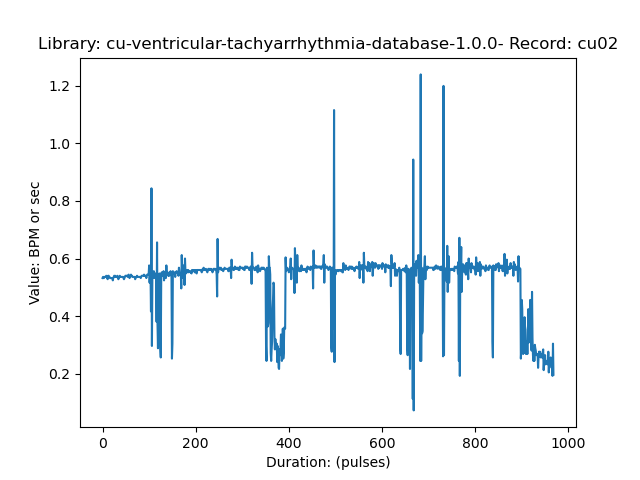
\includegraphics[width=.24\textwidth]{cu-ventricular/cu-ventricular-tachyarrhythmia-database-1.0.0_cu02.png}
		\caption{\gr Δείγμα βιβλιοθήκης \en CU Ventricular Tachyarrhythmia Database \gr (αρχικά δείγματα/καταγραφές)}
	\end{figure}
	\item \en Congestive Heart Failure RR Interval Database: \gr περιέχει 29 καταγραφές και η διάρκεια ποικίλει ανάλογα με την καταγραφή (Σχήμα 4.7).  Οι καταγραφές φαίνεται να περιέχουν μικρότερο ποσοστό θορύβου, γεγονός που αφήνει το σήμα σχετικά ανεπηρέαστο μετά την αφαίρεσή του.\gr
	\begin{figure}
		\centering
		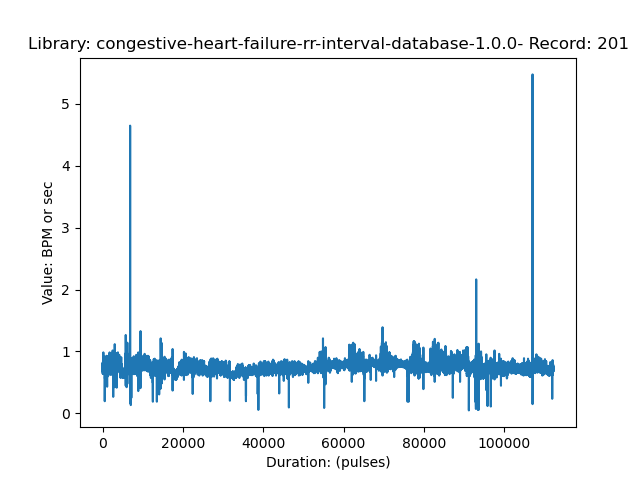
\includegraphics[width=.24\textwidth]{congestive-hf-db/congestive-heart-failure-rr-interval-database-1.0.0_201.png}
		\caption{ \gr Δείγμα βιβλιοθήκης \en Congestive Heart Failure RR Interval Database \gr (αρχικά δείγματα/καταγραφές)}
	\end{figure}
	\item \en CTU-CHB Intrapartum Cardiotocography Database: \gr περιέχει 552 δείγματα από εγκυμονούσες ασθενείς. Οι καταγραφές αποτελούν καρδιοτοκογραφήματα, τα οποία μπορούν να υποστούν επεξεργασία όμοια με τα ηλεκτροκαρδιογραφήματα. Οι καταγραφές έχουν διάρκεια μέχρι και 90 λεπτά (Σχήμα 4.8) πριν τη διαδικασία του ενεργού τοκετού. Η βιβλιοθήκη περιέχει επιπλέον αξιολόγηση διαφορετικών βιοχημικών παραγόντων όπως ο χρόνος κύησης, η πιθανότητα καισαρικής τομής, δεδομένα αναφορικά στη μητέρα και τα φυλετικά χαρακτηριστικά του μωρού. Τα σήματα αποτελούν από τα πιο έντονα σε μορφολογία, λόγω της ιδιαιτερότητας της φυσικής κατάστασης των ασθενών (γυναίκες κατά τη διάρκεια τοκετού, συσπάσεων).
	\begin{figure}
		\centering
		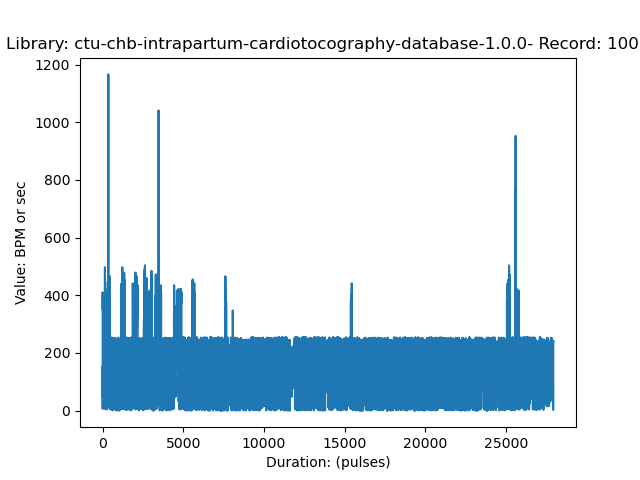
\includegraphics[width=.24\textwidth]{ctu/ctu-chb-intrapartum-cardiotocography-database-1.0.0_1001.png}
		\caption{Δείγμα βιβλιοθήκης \en CTU-CHB Intrapartum Cardiotocography Database \gr (αρχικά δείγματα/καταγραφές)}
	\end{figure}
	\item Fantasia Database: \gr 40 καταγραφές από είκοσι άτομα νεαρής ηλικίας και είκοσι ηλικιωμένους διάρκειας (ίση αναλογία γυναικών και ανδρών) 120 λεπτών. Η καταγραφή πραγματοποιήθηκε ενώ οι εθελοντές βρίσκονται σε κατάσταση ανάπαυσης και παρακολουθούν την ταινία \en Fantasia. \gr Αυτή η βάση δεδομένων αποτελείται από καταγραφές φυσιολογικής καρδιακής λειτουργίας σε κατάσταση ηρεμίας (υγιή άτομα, χωρίς καρδιακές παθήσεις) και συμπεριλήφθηκε για μια πιο ολοκληρωμένη εφαρμογή του αλγορίθμου (Σχήμα 4.9). Όπως παρατηρείται από το αρχικό δείγμα καταγραφών, υπάρχει θόρυβος ο οποίος διαχωρίζεται ευκολότερα μιας και η γεικότερη εικόνα των παλμών είναι ομοιόμορφη, χωρίς εμφάνιση αρρυθμιών.
	\begin{figure}
		\centering
		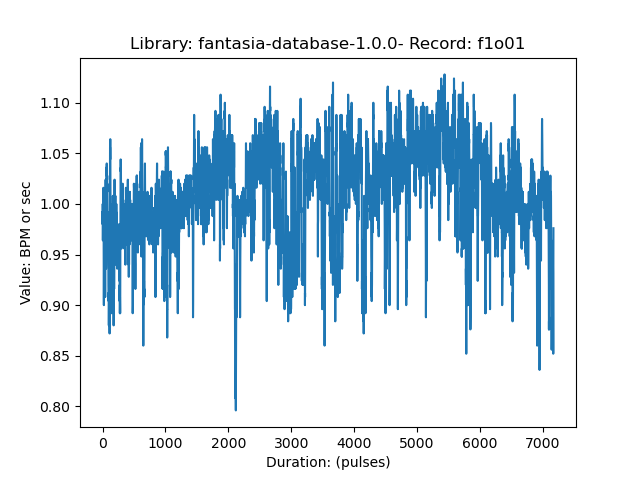
\includegraphics[width=.24\textwidth]{Fantasia/fantasia-database-1.0.0_f1o01.png}
		\caption{\gr Δείγμα βιβλιοθήκης \en Fantasia Database \gr (αρχικά δείγματα/καταγραφές)}
	\end{figure}
	\item Normal Sinus Rhythm RR Interval Database: \gr αποτελείται από 54 καταγραφές (η διάρκεια δεν είναι συγκεκριμένη) από 30 άνδρες ηλικίας 28 έως 76 ετών και 24 γυναίκες ηλικίας 58 έως 73 ετών (Σχήμα 4.10). Τα σήματα καταγράφηκαν σε κατάσταση ηρεμίας (δεν προσδιορίζεται αν οι εθελοντές πάσχουν από κάποια καρδιακή πάθηση) και η διάρκειά τους είναι μεγαλύτερη από 2 ώρες. Η παρουσία έντονων κορυφών παρατηρείται και σε αυτό το σύνολο καταγραφών· δεν αποτελούν, όμως, αρρυθμίες παρά το θόρυβο που αποτυπώθηκε κατά τη διάρκεια της καταγραφής (και αφαιρείται στη συνέχεια), έτσι ώστε να είναι εγκυρότερη η μελέτη, επεξεργασία και αξιολόγηση των σημάτων. 
	\begin{figure}
		\centering
		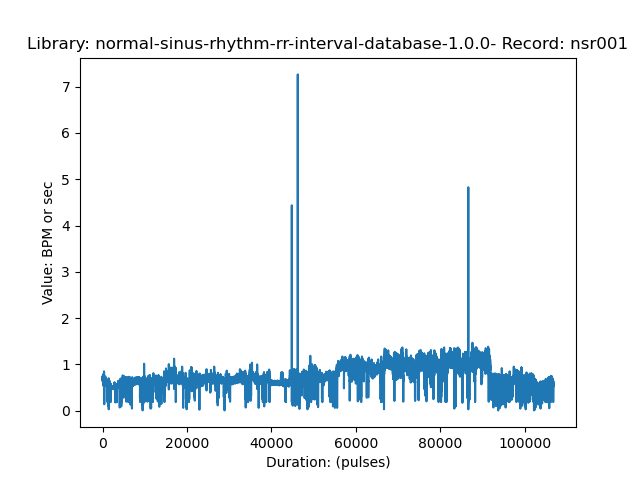
\includegraphics[width=.24\textwidth]{nsr/normal-sinus-rhythm-rr-interval-database-1.0.0_nsr001.png}
		\caption{\gr Δείγμα βιβλιοθήκης \en Normal Sinus Rhythm RR Interval Database \gr (αρχικά δείγματα/καταγραφές)}
	\end{figure}
\end{itemize}
\gr
\par
Παρατηρείται πως τα αρχικά σήματα δεν είναι κατάλληλα προς επεξεργασία στην αρχική τους μορφή. Οι συνθήκες καταγραφής έχουν εισάγει θόρυβο λόγω κακής επαφής των ηλεκτροδίων, κίνησης του ασθενούς ή αποκλίσεις του μηχανήματος. Γίνεται, λοιπόν, αναγκαία μια προεπεξεργασία προκειμένου να "φιλτραριστούν" τα σήματα. Μετά το φιλτράρισμα αυτό, τα σήματα θα είναι ευκολότερο να μελετηθούν, να επεξεργαστούν και να εφαρμοστούν οι αναγκαίες μέθοδοι και να εξαχθούν αποτελέσματα. 
\par
Τα αποτελέσματα αξιολογήθηκαν με βάση τη μορφολογία του σήματος (διάρκεια των καταγραφών, πυκνότητα αρρυθμιών ή/και έκτοπων συστολών). Η διάρκεια των σημάτων και τα διαφορετικά χαρακτηριστικά της κάθε βιβλιοθήκης παρουσιάζονται ξεχωριστά για την καθεμία.

\subsection{Μορφοποίηση πειραμάτων και κώδικας}
Για τη διεξαγωγή αυτών των πειραμάτων δομήθηκε ένας αλγόριθμος, του οποίου ο σκελετός είναι όμοιος με αυτόν που δημιουργήθηκε για το Έργο 82475/110444 - \en HOMore, \gr μιας και τα πειράματα του έργου αποτελούν μέρος αυτής της εργασίας. Η διαδικασία αποσκοπούσε στην απομάκρυνση του θορύβου από κάθε σήμα, όσο αυτό είναι εφικτό, και στη συνέχεια η μελέτη και επεξεργασία των σημάτων μέσω των παραθύρων. Τα παράθυρα δεν είναι τίποτα άλλο παρά τμήματα του ολικού σήματος χωρισμένα σε συγκεκριμένα χρονικά διαστήματα τα οποία καθορίστηκαν τυπικά, ως άξονας σύγκρισης ανάμεσα στις διαφορετικές βιβλιοθήκες (τα μεγέθη τους κυμαίνονται από 15 δευτερόλεπτα έως και 5 λεπτά). Σε κάθε ξεχωριστό παράθυρο, υπολογίζονται οι μετρικές και οι μέθοδοι εκτίμησης εντροπίας και στο τέλος αποτυπώνονται στο γράφημα τα τμήματα/παράθυρα με τις υψηλότερες τιμές της εκάστοτε εξεταζόμενης μετρικής που έφεραν τα υψηλότερα αποτελέσματα. Οι υψηλότερες τιμές αντιστοιχούν σε υψηλό και ακανόνιστο καρδιακό παλμό, δηλαδή αποτελούν τις περιοχές στις οποίες πρέπει να εστιαστεί η προσοχή του μελετητή (ως οι πιο επικίνδυνες).
\subsection{Τα βήματα}
Πιο συγκεκριμένα, τα βήματα του αλγορίθμου είναι τα ακόλουθα:
Σε πρώτο στάδιο, τα σήματα υπέστησαν προεπεξεργασία. Πραγματοποιήθηκε υπολογισμός των διαστημάτων \en RR \gr με βάση τα αρχικά δεδομένα καθώς αυτά δε βρίσκονταν στην επιθυμητή μορφή. Τα δεδομένα τροποποιούνται έτσι ώστε να μπορούν να υποστούν επεξεργασία σε όλες τις βιβλιοθήκες με τον ίδιο τρόπο. Αυτό πραγματοποιείται υπολογίζονταις τις αριθμητικές διαφορές ανάμεσα στους συνεχόμενους παλμούς. Οι βιβλιοθήκες που χρησιμοποιήθηκαν μετρώνται σε δευτερόλεπτα ή σε χτύπους ανά λεπτό. Ως τελικό βήμα καθορίζεται η αφαίρεση του θορύβου για την καλύτερη δυνατή εκτίμηση.
\par
Σε δεύτερο στάδιο, καθορίζονται οι τιμές των παραμέτρων. Η πρώτη παράμετρος είναι το μέγεθος του παραθύρου στο οποίο θα υπολογιστούν οι μέθοδοι και οι μέθοδοι εκτίμησης εντροπίας του \en HRV. \gr Οι δυνατές τιμές που μπορεί να λάβει αυτή η παράμετρος είναι 15, 30, 60, 120, 180, 240 και 300 (αντιστοιχούν σε δευτερόλεπτα). Στις βιβλιοθήκες με πιο σύντομες καταγραφές, το μέγεθος του παραθύρου κυμάνθηκε από 15 σε 60 δευτερόλεπτα. Στη συνέχεια αφαιρέθηκε ο θόρυβος. Ως πρώτο βήμα, απομακρύνθηκαν από το σήμα οι μηδενικές τιμές. Σε μερικές περιπτώσεις η τιμή μηδέν αντιστοιχεί σε απουσία παλμού, ενώ σε άλλες χειροκίνητη αφαίρεση θορύβου από το σήμα, ακόμα και απουσία καταγραφής λόγω κίνησης των ηλεκτροδίων. Αφαιρέθηκαν, επομένως, από το σήμα σε μια προσπάθεια αποφυγής αλλοίωσης των αποτελεσμάτων. Το δεύτερο φίλτρο που χρησιμοποιήθηκε "κόβει" τις ακραίες αριθμητικές τιμές όταν αυτές διαφέρουν περισσότερο από 25 τοις εκατό από τη μέση τιμή του σήματος (δοκιμάστηκαν διαφορετικά κατώφλια ώστε να επιλεχθεί η συγκεκριμένη ως καταλληλότερη). Το τρίτο φίλτρο που χρησιμοποιήθηκε συλλέγει όλες οι κορυφές του σήματος που απέχει αλγεβρικά (τιμή είτε υψηλότερη είτε χαμηλότερη) τουλάχιστον 25\% από τη διάμεσο των τριών προηγούμενων \en RR \gr διαστημάτων. Σε αυτές τις κορυφές έγινε αντικατάσταση της τιμής με τη διάμεσο. Το τέταρτο και τελευταίο φίλτρο είναι αρκετά απλό, καθώς θεωρεί ως θόρυβο τους παλμούς που απέχουν αριθμητικά από τον επόμενό τους περισσότερο από 25 τοις εκατό. Η τιμή αυτών των παλμών αντικαθίσταται σε αυτή την περίπτωση από την τιμή του επόμενου παλμού.
\par
Το τελικό βήμα ήταν η εκτίμηση των μετρικών, των μεθόδων εκτίμησης εντροπίας και των κυματιδίων \en Haar \gr σε κάθε ένα από τα δημιουργούμενα παράθυρα. Οι σκάλες εκτίμησης των κυματιδίων \en Haar \gr κυμαίνοται από δύο έως δέκα, έτσι ώστε να καλυφθεί μεγαλύτερο εύρος τιμών για πιο ακριβείς μετρήσεις (ως μέγιστη τιμή επιλέχθηκε το δέκα, μιας και σε υψηλότερες κλίμακες υπήρξε σύγκλιση των αποτελεσμάτων).
\par
Υπολογίστηκαν επίσης οι μέσες τιμές των μετρικών και μεθόδων για ολόκληρο το σήμα· οι τιμές, δηλαδή, που προέκυψαν από κάθε παράθυρο προστιθέμενες και διαιρεμένες με το μήκος των μετρήσεων του κύματος. Τα γραφήματα δημιουργήθηκαν από τις εκτιμώμενες τιμές του κάθε παραθύρου (κάθε "δείγμα" αποτελεί την τιμή του σήματος ή της εκάστοτε μετρικής και μεθόδου σε ένα συγκεκριμένο παράθυρο). Για τα αποτελέσματα του αλγορίθμου χρησιμοποιήθηκαν όλες οι μετρικές και μέθοδοι και σε κάθε βιβλιοθήκη εντοπίστηκαν οι πιο ακριβείς. Το πόρισμα αυτό προκύπτει από τα πειράματα τα οποία πραγματοποιήθηκαν σε αυτή τη διπλωματική εργασία, έπειτα από παρατήρηση των αποτελεσμάτων. 
\par
Με αυτό το σκεπτικό, επιλέχθηκαν οι υψηλότερες τιμές του πειράματος από την κάθε μία (από την πρώτη έως και τις έξι υψηλότερες) ώστε να προβληθούν στο τελικό διάγραμμα (το πλήθος των επιλεγμένων τιμών μεταβάλλεται εύκολα διότι αποτελεί παράμετρο της εκτέλεσης των πειραμάτων στο τερματικό). Ακόμα, μαζί με αυτές τις μετρικές, στη γραφική παράσταση του κάθε καρδιογραφήματος υπολογίζονται και οι τέσσερις υψηλότερες (σε τιμή) εκτιμήσεις των κυματιδίων \en Haar. \gr  
\par
Συνοπτικά, παραθέτονται τα βήματα του αλγορίθμου για τον εντοπισμό επικίνδυνων περιοχών κατά τη διάρκεια εξαγωγής των πειραμάτων.
\begin{itemize}
	\item Φιλτράρισμα των σημάτων.
	\item Προσδιορισμός των παραθύρων που θα χρησιμοποιηθούν. 
	\item Για κάθε ξεχωριστό παράθυρο, υπολογισμός των μετρικών.
	\item Για κάθε ξεχωριστό παράθυρο, υπολογισμός των μεθόδων εκτίμησης εντροπίας.
	\item Επιλογή των παραθύρων με τις υψηλότερες τιμές μετρικών ή μεθόδων.  
	\item Υπολογισμός των συντεταγμένων των συγκεκριμένων παραθύρων (τα παράθυρα είναι ισομεγέθη, στις περισσότερες περιπτώσεις 60 δευτερόλεπτα).
	\item Υπολογισμός γραφήματος (οι επικίνδυνες περιοχές διαφοροποιούνται για να είναι ευκολότερη η εστίαση του μελετητή ή του ιατρικού ερευνητή/γιατρού). Συνολικά για κάθε σήμα παράγονται γραφήματα με τις εκτιμώμενες επικίνδυνες περιοχές τόσο των μετρικών όσο και των κυματιδίων \en Haar. \gr Η διαδικασία αυτή επαναλαμβάνεται για όλα τα δείγματα κάθε βιβλιοθήκης. 
\end{itemize}


\subsection{Καθορισμός παραμέτρων}
Οι αναγκαίες παράμετροι στη διεκπεραίωση των ερευνητικών πειραμάτων ήταν οι ακόλουθες:
\begin{itemize}
	\item το μέγεθος του παραθύρου επεξεργασίας που λαμβάνει την τιμή του χρονικού διαστήματος σε δευτερόλεπτα (όνομα παραμέτρου στον κώδικα: $window size$)
	\item στη μέθοδο αφαίρεσης θορύβου, ο συνυπολογισμός των τριών προηγούμενων δειγμάτων από τα οποία υπολογίζεται το ποσοστό διαφοράς από τη διάμεσο (όνομα παραμέτρου στον κώδικα: $n previous values$) 
	\item το κατώφλι που επιλέχθηκε σε κάθε φίλτρο αφαίρεσης θορύβου (όνομα παραμέτρου στον κώδικα: $threshold$)
	\item η σκάλα ή επίπεδο στον υπολογισμό των κυματιδίων \en Haar \gr (όνομα παραμέτρου στον κώδικα: $scale$)
	\item η παράμετρος διάστασης του \en m-\gr διάστατου χώρου στον οποίο ενσωματώνεται το σήμα στις μεθόδους \en Approximate Entropy, Sample Entropy, Bubble Entropy \gr (όνομα παραμέτρου στον κώδικα: $m$)
	\item η παράμετρος κλίμακας (φίλτρο θορύβου) στις μεθόδους \en Approximate Entropy, Sample Entropy, Bubble Entropy \gr (όνομα παραμέτρου στον κώδικα: $r$)
\end{itemize}

\par
Συνοπτικά, η πορεία επεξεργασίας των σημάτων και ο αλγόριθμος παρουσιάζονται στο ακόλουθο διάγραμμα (Σχήμα 4.11):
\begin{figure}
	\centering
	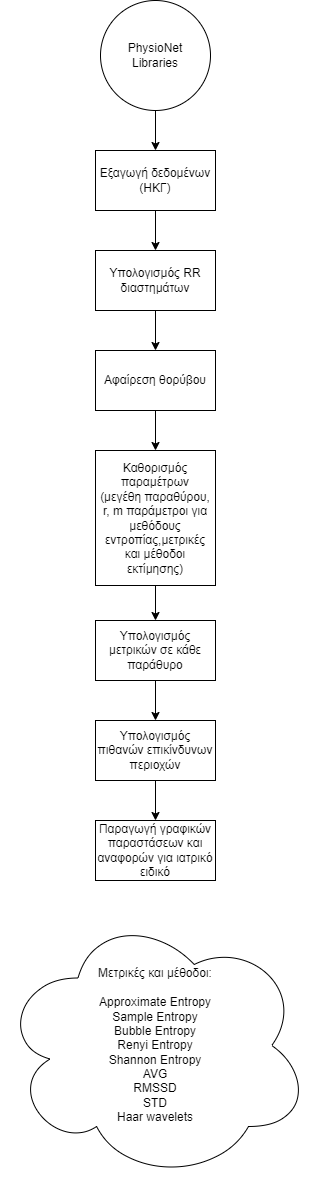
\includegraphics[width=0.4\textwidth]{Algorithm.png}
	\caption{Διαγραμματική απεικόνιση του αλορίθμου επεξεργασίας καρδιακών σημάτων}
\end{figure}


\section{Αποτελέσματα πειραματικής ανάλυσης}
Ο σχολιασμός κάθε βιβλιοθήκης θα παρατεθεί στη συνέχεια εξ ολοκλήρου για την κάθε μία, από την παραγωγή των διαγραμμάτων έως και το σχολιασμό των αποτελεσμάτων. 
\par 
\textbf{Σημείωση:} Στη συνέχεια παρουσιάζεται αυξημένο πλήθος πειραμάτων και κατά συνέπεια διαγραμμάτων, κάτι που μπορεί να κουράσει τον αναγνώστη. Ο όγκος αυτός δεν ήταν δυνατό να περιοριστεί διότι αποτελεί απόδειξη της λειτουργίας και απόδοσης του αλγορίθμου. Για αυτό το σκοπό, στο τέλος του κεφαλαίου πραγματοποιείται μια πιο συνοπτική ανακεφαλαίωση, ώστε να γίνει ευκολότερη η ερμηνεία των αποτελεσμάτων.
\par
\subsection{\en Long Term AF Database \gr}
Σε αυτή τη βιβλιοθήκη τα μεγέθη των παραθύρων που εφαρμόστηκαν (σε δευτερόλεπτα) ήταν τα [60, 120, 240, 300]. Τα δείγματα αυτής της βιβλιοθήκης αποτελούν αρνητικά παραδείγματα, διότι η διάρκεια των σημάτων είναι εκτενής. Αυτό, όμως που καθιστά τις εκτιμήσεις δύσκολες και πιθανώς άστοχες είναι η ένταση των παλμών στις καταγραφές. Τα σήματα είναι δασώδη, ή πριονωτά, κάτι που καθιστά το σήμα δύσκολο να ερμηνευθεί. Λίγες είναι οι περιπτώσεις στις οποίες τα δείγματα ευνοούν τις προβλέψεις και εκτιμήσεις του αλγορίθμου. 
Τα σήματα αρχικά είχαν την εξής εικόνα (χωρίς φιλτράρισμα θορύβου) (Σχήμα 4,12): 
\begin{figure}
	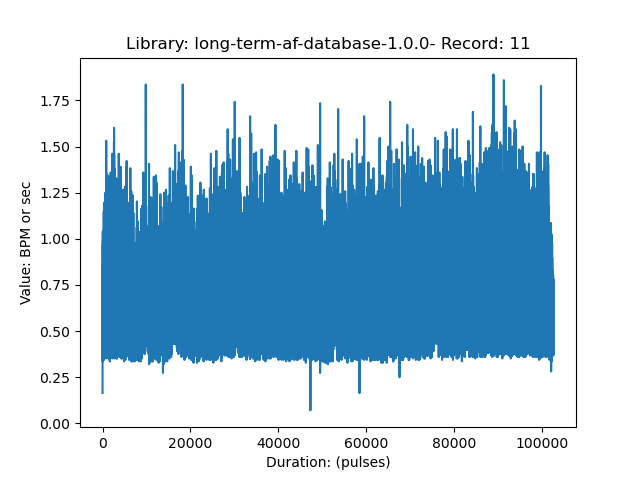
\includegraphics[width=.24\textwidth]{long-term-af-db/long-term-af-database-1.0.0_11.png}\hfill
	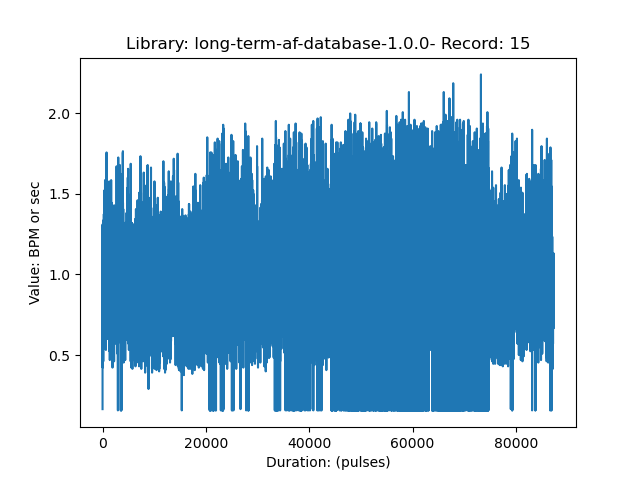
\includegraphics[width=.24\textwidth]{long-term-af-db/long-term-af-database-1.0.0_15.png}\hfill
	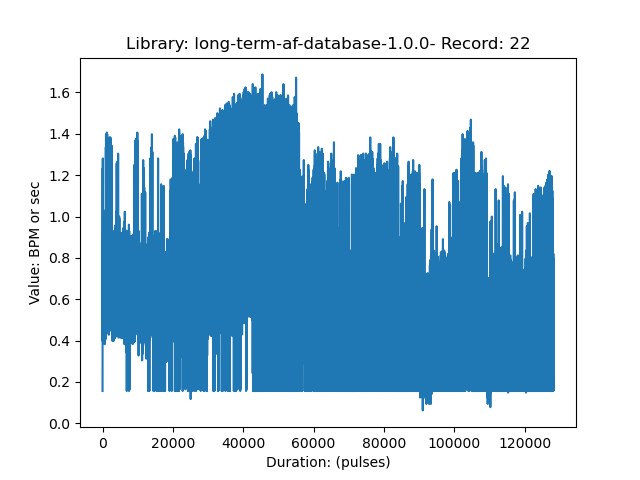
\includegraphics[width=.24\textwidth]{long-term-af-db/long-term-af-database-1.0.0_22.png}\hfill
	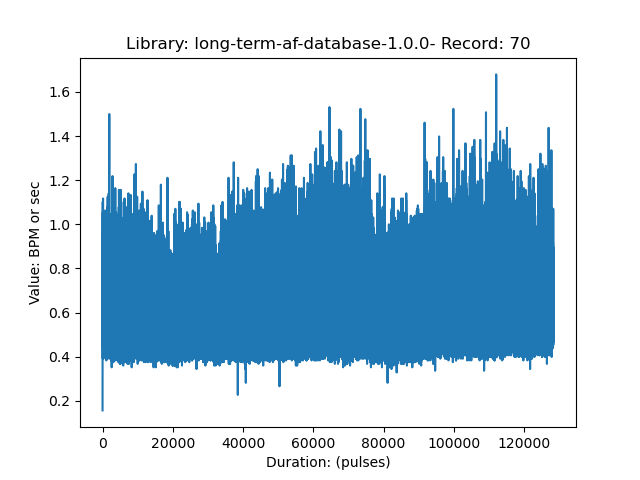
\includegraphics[width=.24\textwidth]{long-term-af-db/long-term-af-database-1.0.0_70.png}\hfill
	\\[\smallskipamount]
	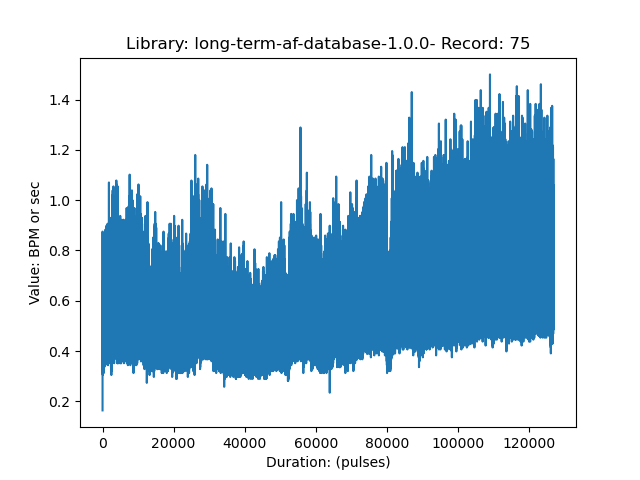
\includegraphics[width=.24\textwidth]{long-term-af-db/long-term-af-database-1.0.0_75.png}\hfill
	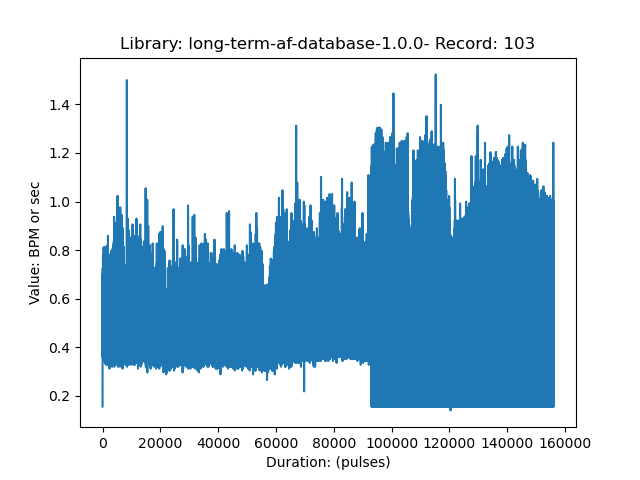
\includegraphics[width=.24\textwidth]{long-term-af-db/long-term-af-database-1.0.0_103.png}\hfill
	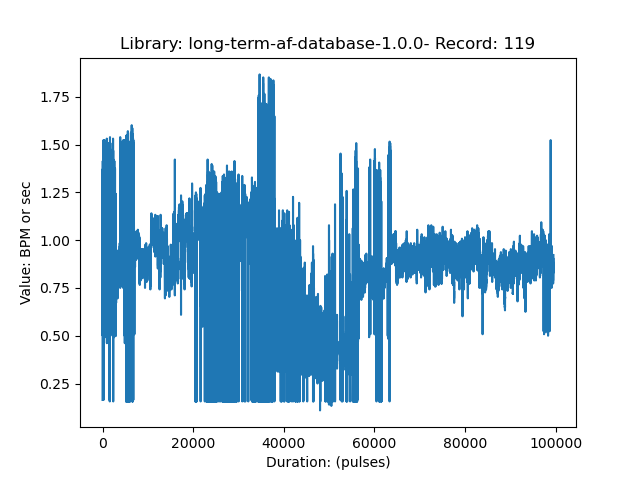
\includegraphics[width=.24\textwidth]{long-term-af-db/long-term-af-database-1.0.0_119.png}\hfill
	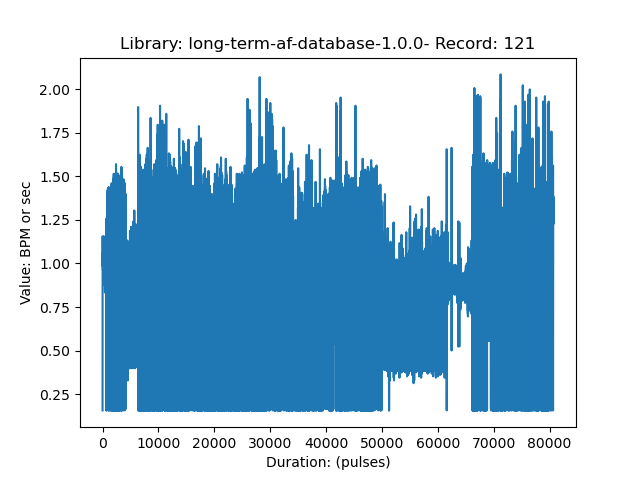
\includegraphics[width=.24\textwidth]{long-term-af-db/long-term-af-database-1.0.0_121.png}\hfill
	\\[\smallskipamount]
	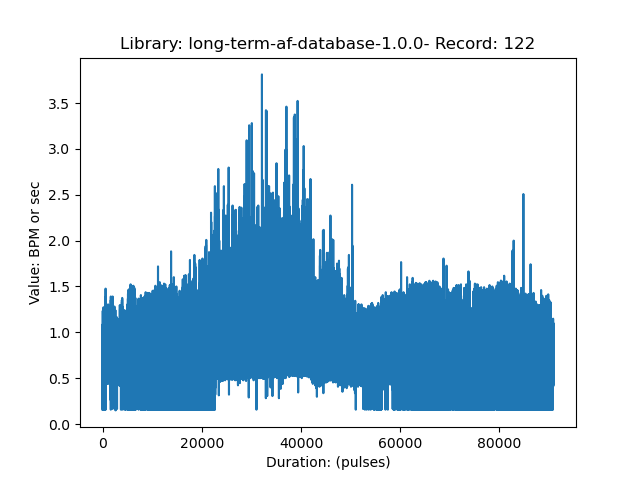
\includegraphics[width=.24\textwidth]{long-term-af-db/long-term-af-database-1.0.0_122.png}\hfill
	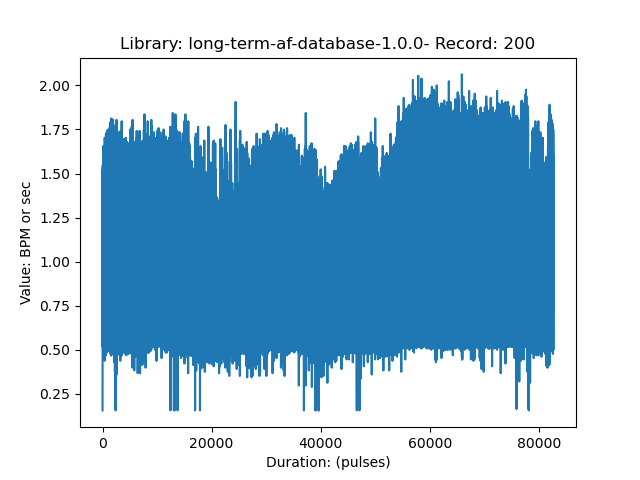
\includegraphics[width=.24\textwidth]{long-term-af-db/long-term-af-database-1.0.0_200.png}\hfill
	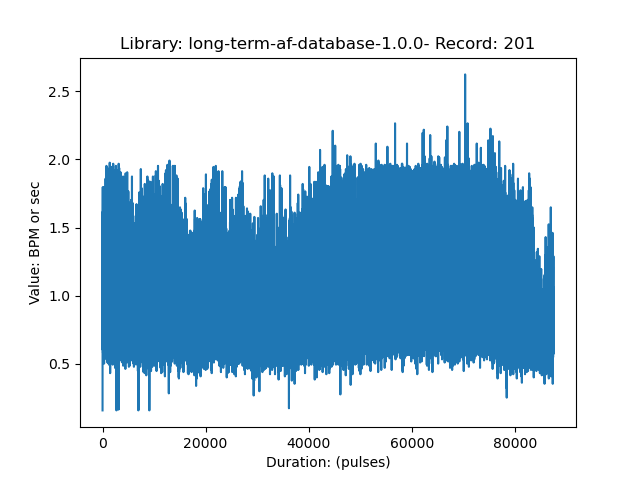
\includegraphics[width=.24\textwidth]{long-term-af-db/long-term-af-database-1.0.0_201.png}\hfill
	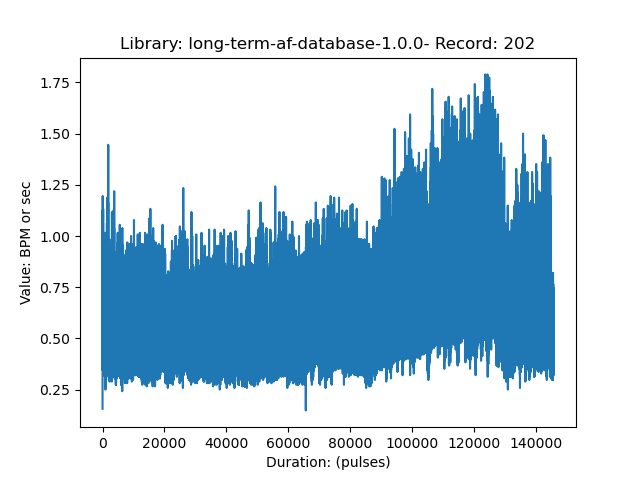
\includegraphics[width=.24\textwidth]{long-term-af-db/long-term-af-database-1.0.0_202.png}\hfill
	\caption{Συλλογή αποτελεσμάτων από τη βιβλιοθήκη \en Long Term AF Database \gr (αρχικά δείγματα/καταγραφές)}
\end{figure}
Μετά την εφαρμογή του αλγορίθμου τα αποτελέσματα ήταν τα εξής:
\begin{itemize}
	\item \en ApEn: \gr
	Τα αποτελέσματα αυτής της μεθόδου εκτίμησης εντροπίας δεν είναι εύστοχες. Κανένα από τα μεγέθη των παραθύρων δεν βελτιώνει ιδιαίτερα τις προβλέψεις. Ένα επιπλέον αρνητικό αποτέλεσμα αυτής της μεθόδου είναι πως όσο τα μεγέθη των παραθύρων μεταβάλλονται οι εκτιμήσεις της μεθόδου δεν παραμένουν σταθερές. Αυτό σημαίνει πως όσο τα παράθυρα αλλάζουν, η μέθοδος δε συνεχίζει να εστιάζει στην ίδια περιοχή, είτε η περιοχή είναι πιθανώς επικίνδυνη είτε όχι. 
	\par
	Μερικά ενδεικτικά δείγματα παρουσιάζονται στα Σχήματα 4.13 (παράδειγμα που υποδεικνύει την αλλαγή των "επικίνδυνων περιοχών" όσο τα παράθυρα αλλάζουν) και 4.14 (ενδεικτικά αποτελέσματα των εκτιμήσεων της \en ApEn) \gr: 
	\begin{figure}
		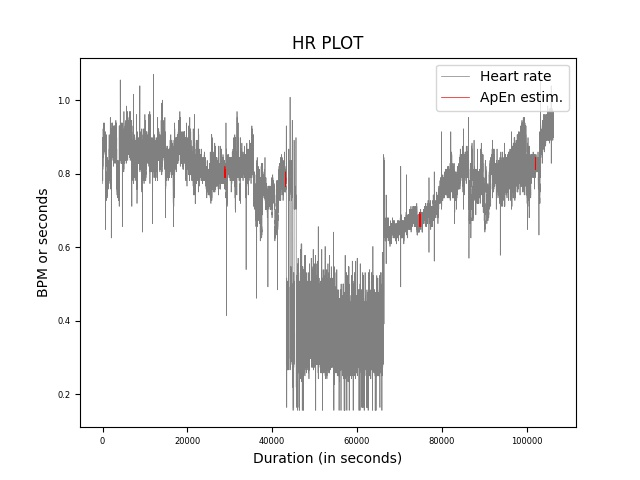
\includegraphics[width=.24\textwidth]{ApEn-long-term-af-db/long-term-af-database-1.0.0_00_60sec.jpeg}\hfill
		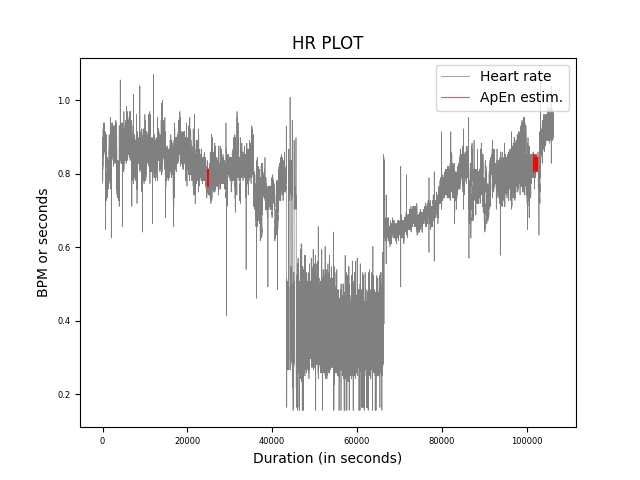
\includegraphics[width=.24\textwidth]{ApEn-long-term-af-db/long-term-af-database-1.0.0_00_120sec.jpeg}\hfill
		\includegraphics[width=.24\textwidth]{ApEn-long-term-af-db/long-term-af-database-1.0.0_00_180sec.jpeg}\hfill
		\centering
		\includegraphics[width=.24\textwidth]{ApEn-long-term-af-db/long-term-af-database-1.0.0_00_240sec.jpeg}\hfill
		\caption{Συλλογή αποτελεσμάτων από τη βιβλιοθήκη \en Long Term AF Database \gr για τη μετρική \en ApEn \gr (αλλαγή μεγέθους παραθύρων)}
	\end{figure}
	\begin{figure}
		\includegraphics[width=.24\textwidth]{ApEn-long-term-af-db/long-term-af-database-1.0.0_15_240sec.jpeg}\hfill
		\includegraphics[width=.24\textwidth]{ApEn-long-term-af-db/long-term-af-database-1.0.0_16_240sec.jpeg}\hfill
		\includegraphics[width=.24\textwidth]{ApEn-long-term-af-db/long-term-af-database-1.0.0_17_240sec.jpeg}\hfill
		\includegraphics[width=.24\textwidth]{ApEn-long-term-af-db/long-term-af-database-1.0.0_18_240sec.jpeg}\hfill
		\\[\smallskipamount]
		\includegraphics[width=.24\textwidth]{ApEn-long-term-af-db/long-term-af-database-1.0.0_19_240sec.jpeg}\hfill
		\includegraphics[width=.24\textwidth]{ApEn-long-term-af-db/long-term-af-database-1.0.0_20_240sec.jpeg}\hfill
		\includegraphics[width=.24\textwidth]{ApEn-long-term-af-db/long-term-af-database-1.0.0_21_240sec.jpeg}\hfill
		\includegraphics[width=.24\textwidth]{ApEn-long-term-af-db/long-term-af-database-1.0.0_22_240sec.jpeg}\hfill
		\\[\smallskipamount]
		\includegraphics[width=.24\textwidth]{ApEn-long-term-af-db/long-term-af-database-1.0.0_23_240sec.jpeg}\hfill
		\includegraphics[width=.24\textwidth]{ApEn-long-term-af-db/long-term-af-database-1.0.0_24_240sec.jpeg}\hfill
		\includegraphics[width=.24\textwidth]{ApEn-long-term-af-db/long-term-af-database-1.0.0_25_240sec.jpeg}\hfill
		\includegraphics[width=.24\textwidth]{ApEn-long-term-af-db/long-term-af-database-1.0.0_26_240sec.jpeg}\hfill
		\caption{Συλλογή αποτελεσμάτων από τη βιβλιοθήκη \en Long Term AF Database \gr για τη μετρική \en ApEn \gr)}
	\end{figure}
	\item \en AVG: \gr Η συγκεκριμένη μέθοδος σε αντίθεση με την προηγούμενη έχει πιο εύστοχα αποτελέσματα και μεγαλύτερη σταθερότητα (Σχήμα 4.15). Υπάρχουν περιπτώσεις στις οποίες οι εκτιμήσεις ταυτίζονται με περιοχές-παλμούς με μη φυσιολογική καρδιακή λειτουργία, εξαιτίας της μορφολογίας του σήματος δεν είναι επιτυχείς (Σχήμα 4.16).
	\begin{figure}
		\includegraphics[width=.24\textwidth]{AVG-long-term-af-db/long-term-af-database-1.0.0_00_60sec.jpeg}\hfill
		\includegraphics[width=.24\textwidth]{AVG-long-term-af-db/long-term-af-database-1.0.0_00_120sec.jpeg}\hfill
		\includegraphics[width=.24\textwidth]{AVG-long-term-af-db/long-term-af-database-1.0.0_00_180sec.jpeg}\hfill
		\includegraphics[width=.24\textwidth]{AVG-long-term-af-db/long-term-af-database-1.0.0_00_240sec.jpeg}\hfill
		\centering
		\includegraphics[width=.24\textwidth]{AVG-long-term-af-db/long-term-af-database-1.0.0_00_300sec.jpeg}\hfill
		\caption{Συλλογή αποτελεσμάτων από τη βιβλιοθήκη \en Long Term AF Database \gr για τη μετρική \en AVG \gr (αλλαγή μεγέθους παραθύρων)}
	\end{figure}
	\begin{figure}
		\includegraphics[width=.24\textwidth]{AVG-long-term-af-db/long-term-af-database-1.0.0_15_300sec.jpeg}\hfill
		\includegraphics[width=.24\textwidth]{AVG-long-term-af-db/long-term-af-database-1.0.0_16_300sec.jpeg}\hfill
		\includegraphics[width=.24\textwidth]{AVG-long-term-af-db/long-term-af-database-1.0.0_17_300sec.jpeg}\hfill
		\includegraphics[width=.24\textwidth]{AVG-long-term-af-db/long-term-af-database-1.0.0_18_300sec.jpeg}\hfill
		\\[\smallskipamount]
		\includegraphics[width=.24\textwidth]{AVG-long-term-af-db/long-term-af-database-1.0.0_19_300sec.jpeg}\hfill
		\includegraphics[width=.24\textwidth]{AVG-long-term-af-db/long-term-af-database-1.0.0_20_300sec.jpeg}\hfill
		\includegraphics[width=.24\textwidth]{AVG-long-term-af-db/long-term-af-database-1.0.0_21_300sec.jpeg}\hfill
		\includegraphics[width=.24\textwidth]{AVG-long-term-af-db/long-term-af-database-1.0.0_22_300sec.jpeg}\hfill
		\\[\smallskipamount]
		\includegraphics[width=.24\textwidth]{AVG-long-term-af-db/long-term-af-database-1.0.0_23_300sec.jpeg}\hfill
		\includegraphics[width=.24\textwidth]{AVG-long-term-af-db/long-term-af-database-1.0.0_24_300sec.jpeg}\hfill
		\includegraphics[width=.24\textwidth]{AVG-long-term-af-db/long-term-af-database-1.0.0_25_300sec.jpeg}\hfill
		\includegraphics[width=.24\textwidth]{AVG-long-term-af-db/long-term-af-database-1.0.0_26_300sec.jpeg}\hfill
		\caption{Συλλογή αποτελεσμάτων από τη βιβλιοθήκη \en Long Term AF Database \gr για τη μετρική \en AVG \gr)}
	\end{figure}
	\item  \en Bubble: \gr Σε αντίθεση με την \en ApEn \gr σε αυτή τη μέθοδο παρατηρείται πως όσο το μέγεθος του παραθύρου αυξάνεται, οι προβλέψεις του αλγορίθμου γίνονται πιο εύστοχες (Σχήμα 4.17), χωρίς αυτό να αναιρεί τη μη σταθερότητα της μεθόδου με την αλλαγή των μεγεθών σε κάθε δείγμα. Παρόλα αυτά τα αποτελέσματα είναι πιο ενθαρρυντικά (Σχήμα 4.18). 
	\begin{figure}
		\includegraphics[width=.24\textwidth]{Bubble-long-term-af-db/long-term-af-database-1.0.0_00_60sec.jpeg}\hfill
		\includegraphics[width=.24\textwidth]{Bubble-long-term-af-db/long-term-af-database-1.0.0_00_120sec.jpeg}\hfill
		\includegraphics[width=.24\textwidth]{Bubble-long-term-af-db/long-term-af-database-1.0.0_00_180sec.jpeg}\hfill
		\includegraphics[width=.24\textwidth]{Bubble-long-term-af-db/long-term-af-database-1.0.0_00_240sec.jpeg}\hfill
		\centering
		\includegraphics[width=.24\textwidth]{Bubble-long-term-af-db/long-term-af-database-1.0.0_00_300sec.jpeg}\hfill
		\caption{Συλλογή αποτελεσμάτων από τη βιβλιοθήκη \en Long Term AF Database \gr για τη μετρική \en Bubble \gr (αλλαγή μεγέθους παραθύρων)}
	\end{figure}
	\begin{figure}
		\includegraphics[width=.24\textwidth]{Bubble-long-term-af-db/long-term-af-database-1.0.0_15_240sec.jpeg}\hfill
		\includegraphics[width=.24\textwidth]{Bubble-long-term-af-db/long-term-af-database-1.0.0_16_240sec.jpeg}\hfill
		\includegraphics[width=.24\textwidth]{Bubble-long-term-af-db/long-term-af-database-1.0.0_17_240sec.jpeg}\hfill
		\includegraphics[width=.24\textwidth]{Bubble-long-term-af-db/long-term-af-database-1.0.0_18_240sec.jpeg}\hfill
		\\[\smallskipamount]
		\includegraphics[width=.24\textwidth]{Bubble-long-term-af-db/long-term-af-database-1.0.0_19_240sec.jpeg}\hfill
		\includegraphics[width=.24\textwidth]{Bubble-long-term-af-db/long-term-af-database-1.0.0_20_240sec.jpeg}\hfill
		\includegraphics[width=.24\textwidth]{Bubble-long-term-af-db/long-term-af-database-1.0.0_21_240sec.jpeg}\hfill
		\includegraphics[width=.24\textwidth]{Bubble-long-term-af-db/long-term-af-database-1.0.0_22_240sec.jpeg}\hfill
		\\[\smallskipamount]
		\includegraphics[width=.24\textwidth]{Bubble-long-term-af-db/long-term-af-database-1.0.0_23_240sec.jpeg}\hfill
		\includegraphics[width=.24\textwidth]{Bubble-long-term-af-db/long-term-af-database-1.0.0_24_240sec.jpeg}\hfill
		\includegraphics[width=.24\textwidth]{Bubble-long-term-af-db/long-term-af-database-1.0.0_25_240sec.jpeg}\hfill
		\includegraphics[width=.24\textwidth]{Bubble-long-term-af-db/long-term-af-database-1.0.0_26_240sec.jpeg}\hfill
		\caption{Συλλογή αποτελεσμάτων από τη βιβλιοθήκη \en Long Term AF Database \gr για τη μετρική \en Bubble \gr)}
	\end{figure}
	\item \en Rényi: \gr Η απόδοση αυτής της μετρικής θεωρείται μέτρια. Αυτό αιτιολογείται από τη μορφολογία του σήματος. Ενώ εντοπίζονται περιοχές που χαρακτηρίζονται ως μη φυσιολογικές, τα δείγματα βρίσκονται πολύ συχνά σε παρόμοια κατάσταση με αποτέλεσμα να μην εντοπίζονται οι πιο ακραίες από τις περιοχές. Αυτό που παρατηρείται είναι η εστίαση της μετρικής στις περιοχές με τις χαμηλότερες αριθμητικά τιμές και όχι στις υψηλές (Σχήματα 4.19, 4.20). 
	\begin{figure}
		\includegraphics[width=.24\textwidth]{Renyi-long-term-af/long-term-af-database-1.0.0_01_60sec.jpeg}\hfill
		\includegraphics[width=.24\textwidth]{Renyi-long-term-af/long-term-af-database-1.0.0_01_120sec.jpeg}\hfill
		\includegraphics[width=.24\textwidth]{Renyi-long-term-af/long-term-af-database-1.0.0_01_180sec.jpeg}\hfill
		\includegraphics[width=.24\textwidth]{Renyi-long-term-af/long-term-af-database-1.0.0_01_240sec.jpeg}\hfill
		\centering
		\includegraphics[width=.24\textwidth]{Renyi-long-term-af/long-term-af-database-1.0.0_01_300sec.jpeg}\hfill
		\caption{Συλλογή αποτελεσμάτων από τη βιβλιοθήκη \en Long Term AF Database \gr για τη μετρική \en Rényi \gr (αλλαγή μεγέθους παραθύρων)}
	\end{figure}
	\begin{figure}
		\includegraphics[width=.24\textwidth]{Renyi-long-term-af/long-term-af-database-1.0.0_00_300sec.jpeg}\hfill
		\includegraphics[width=.24\textwidth]{Renyi-long-term-af/long-term-af-database-1.0.0_105_240sec.jpeg}\hfill
		\includegraphics[width=.24\textwidth]{Renyi-long-term-af/long-term-af-database-1.0.0_116_300sec.jpeg}\hfill
		\includegraphics[width=.24\textwidth]{Renyi-long-term-af/long-term-af-database-1.0.0_119_240sec.jpeg}\hfill
		\includegraphics[width=.24\textwidth]{Renyi-long-term-af/long-term-af-database-1.0.0_120_300sec.jpeg}\hfill
		\\[\smallskipamount]
		\includegraphics[width=.24\textwidth]{Renyi-long-term-af/long-term-af-database-1.0.0_201_180sec.jpeg}\hfill
		\includegraphics[width=.24\textwidth]{Renyi-long-term-af/long-term-af-database-1.0.0_05_60sec.jpeg}\hfill
		\includegraphics[width=.24\textwidth]{Renyi-long-term-af/long-term-af-database-1.0.0_74_60sec.jpeg}\hfill
		\includegraphics[width=.24\textwidth]{Renyi-long-term-af/long-term-af-database-1.0.0_00_300sec.jpeg}\hfill
		\\[\smallskipamount]
		\includegraphics[width=.24\textwidth]{Renyi-long-term-af/long-term-af-database-1.0.0_08_120sec.jpeg}\hfill
		\includegraphics[width=.24\textwidth]{Renyi-long-term-af/long-term-af-database-1.0.0_122_60sec.jpeg}\hfill
		\includegraphics[width=.24\textwidth]{Renyi-long-term-af/long-term-af-database-1.0.0_206_60sec.jpeg}\hfill
		\includegraphics[width=.24\textwidth]{Renyi-long-term-af/long-term-af-database-1.0.0_208_300sec.jpeg}\hfill
		\caption{Συλλογή αποτελεσμάτων από τη βιβλιοθήκη \en Long Term AF Database \gr για τη μετρική \en Rényi \gr)}
	\end{figure}
	
	\item \en RMSSD: \gr Ίσως η μετρική με τα καλύτερα αποτελέσματα. Σταθερή όσο τα μεγέθη παραθύρων αλλάζουν (συγκλίνουν στις περισσότερες περιπτώσεις στην ίδια περιοχή εκτίμησης) και στην πλειοψηφία των δειγμάτων εντοπίζονται οι περιοχές με μεγαλύτερη πιθανότητα μη φυσιολογικής καρδιακής δραστηριότητας, αν και αυτό δε σημαίνει πολλά, λόγω της μόνιμης κατάστασης του σήματος. Ενδεικτικά αποτελέσματα των εκτιμήσεων αυτής της μετρικής εμφανίζονται στα Σχήματα 4.21, 4.22.
	
	\begin{figure}
		\includegraphics[width=.24\textwidth]{RMSSD-long-term-af-db/long-term-af-database-1.0.0_00_60sec.jpeg}\hfill
		\includegraphics[width=.24\textwidth]{RMSSD-long-term-af-db/long-term-af-database-1.0.0_00_120sec.jpeg}\hfill
		\includegraphics[width=.24\textwidth]{RMSSD-long-term-af-db/long-term-af-database-1.0.0_00_180sec.jpeg}\hfill
		\includegraphics[width=.24\textwidth]{RMSSD-long-term-af-db/long-term-af-database-1.0.0_00_240sec.jpeg}\hfill
		\centering
		\includegraphics[width=.24\textwidth]{RMSSD-long-term-af-db/long-term-af-database-1.0.0_00_300sec.jpeg}\hfill
		\caption{Συλλογή αποτελεσμάτων από τη βιβλιοθήκη \en Long Term AF Database \gr για τη μετρική \en RMSSD \gr (αλλαγή μεγέθους παραθύρων)}
	\end{figure}
	\begin{figure}
		\includegraphics[width=.24\textwidth]{RMSSD-long-term-af-db/long-term-af-database-1.0.0_15_240sec.jpeg}\hfill
		\includegraphics[width=.24\textwidth]{RMSSD-long-term-af-db/long-term-af-database-1.0.0_16_240sec.jpeg}\hfill
		\includegraphics[width=.24\textwidth]{RMSSD-long-term-af-db/long-term-af-database-1.0.0_17_240sec.jpeg}\hfill
		\includegraphics[width=.24\textwidth]{RMSSD-long-term-af-db/long-term-af-database-1.0.0_18_240sec.jpeg}\hfill
		\\[\smallskipamount]
		\includegraphics[width=.24\textwidth]{RMSSD-long-term-af-db/long-term-af-database-1.0.0_19_240sec.jpeg}\hfill
		\includegraphics[width=.24\textwidth]{RMSSD-long-term-af-db/long-term-af-database-1.0.0_20_240sec.jpeg}\hfill
		\includegraphics[width=.24\textwidth]{RMSSD-long-term-af-db/long-term-af-database-1.0.0_21_240sec.jpeg}\hfill
		\includegraphics[width=.24\textwidth]{RMSSD-long-term-af-db/long-term-af-database-1.0.0_22_240sec.jpeg}\hfill
		\\[\smallskipamount]
		\includegraphics[width=.24\textwidth]{RMSSD-long-term-af-db/long-term-af-database-1.0.0_23_240sec.jpeg}\hfill
		\includegraphics[width=.24\textwidth]{RMSSD-long-term-af-db/long-term-af-database-1.0.0_24_240sec.jpeg}\hfill
		\includegraphics[width=.24\textwidth]{RMSSD-long-term-af-db/long-term-af-database-1.0.0_25_240sec.jpeg}\hfill
		\includegraphics[width=.24\textwidth]{RMSSD-long-term-af-db/long-term-af-database-1.0.0_26_240sec.jpeg}\hfill
		\caption{Συλλογή αποτελεσμάτων από τη βιβλιοθήκη \en Long Term AF Database \gr για τη μετρική \en RMSSD \gr)}
	\end{figure}
	
	\item \en SampEn: \gr Η εικόνα που αποδίδει παραπέμπει στην εικόνα της \en ApEn \gr με την ίδια αστάθεια και άστοχη εκτίμηση. Αυτή η διαπίστωση είναι κάτι που εύκολα διακρίνεται και "με το μάτι" από τα αποτελέσματα των διαγραμμάτων στα Σχήματα 4.23, 4.24.
	
	
	\begin{figure}
		\includegraphics[width=.24\textwidth]{SampEn-long-term-af-db/long-term-af-database-1.0.0_00_60sec.jpeg}\hfill
		\includegraphics[width=.24\textwidth]{SampEn-long-term-af-db/long-term-af-database-1.0.0_00_120sec.jpeg}\hfill
		\includegraphics[width=.24\textwidth]{SampEn-long-term-af-db/long-term-af-database-1.0.0_00_180sec.jpeg}\hfill
		\includegraphics[width=.24\textwidth]{SampEn-long-term-af-db/long-term-af-database-1.0.0_00_240sec.jpeg}\hfill
		\centering
		\includegraphics[width=.24\textwidth]{SampEn-long-term-af-db/long-term-af-database-1.0.0_00_300sec.jpeg}\hfill
		\caption{Συλλογή αποτελεσμάτων από τη βιβλιοθήκη \en Long Term AF Database \gr για τη μετρική \en SampEn \gr (αλλαγή μεγέθους παραθύρων)}
	\end{figure}
	\begin{figure}
		\includegraphics[width=.24\textwidth]{SampEn-long-term-af-db/long-term-af-database-1.0.0_15_300sec.jpeg}\hfill
		\includegraphics[width=.24\textwidth]{SampEn-long-term-af-db/long-term-af-database-1.0.0_16_300sec.jpeg}\hfill
		\includegraphics[width=.24\textwidth]{SampEn-long-term-af-db/long-term-af-database-1.0.0_17_300sec.jpeg}\hfill
		\includegraphics[width=.24\textwidth]{SampEn-long-term-af-db/long-term-af-database-1.0.0_18_300sec.jpeg}\hfill
		\\[\smallskipamount]
		\includegraphics[width=.24\textwidth]{SampEn-long-term-af-db/long-term-af-database-1.0.0_19_300sec.jpeg}\hfill
		\includegraphics[width=.24\textwidth]{SampEn-long-term-af-db/long-term-af-database-1.0.0_20_300sec.jpeg}\hfill
		\includegraphics[width=.24\textwidth]{SampEn-long-term-af-db/long-term-af-database-1.0.0_21_300sec.jpeg}\hfill
		\includegraphics[width=.24\textwidth]{SampEn-long-term-af-db/long-term-af-database-1.0.0_22_300sec.jpeg}\hfill
		\\[\smallskipamount]
		\includegraphics[width=.24\textwidth]{SampEn-long-term-af-db/long-term-af-database-1.0.0_23_300sec.jpeg}\hfill
		\includegraphics[width=.24\textwidth]{SampEn-long-term-af-db/long-term-af-database-1.0.0_24_300sec.jpeg}\hfill
		\includegraphics[width=.24\textwidth]{SampEn-long-term-af-db/long-term-af-database-1.0.0_25_300sec.jpeg}\hfill
		\includegraphics[width=.24\textwidth]{SampEn-long-term-af-db/long-term-af-database-1.0.0_26_300sec.jpeg}\hfill
		\caption{Συλλογή αποτελεσμάτων από τη βιβλιοθήκη \en Long Term AF Database \gr για τη μετρική \en SampEn \gr)}
	\end{figure}
	
	\item \en Shannon: \gr Τα αποτελέσματα εκτίμησης αυτής της μεθόδου βρίσκονται σε μία μέση κατάσταση. Υπάρχουν τόσο δείγματα που εντοπίζουν παλμούς με πολύ υψηλές τιμές όσο και περιπτώσεις που οι εκτιμήσεις είναι εντελώς άστοχες. Ακόμα, η μέθοδος συγκλίνει στις περισσότερες περιπτώσεις στην ίδια περιοχή, ανεξαρτήτως του μεγέθους του παραθύρου (Σχήμα 4.25, Σχήμα 4.26). 
	
	\begin{figure}
		\includegraphics[width=.24\textwidth]{Shannon-long-term-af-db/long-term-af-database-1.0.0_15_60sec.jpeg}\hfill
		\includegraphics[width=.24\textwidth]{Shannon-long-term-af-db/long-term-af-database-1.0.0_15_120sec.jpeg}\hfill
		\includegraphics[width=.24\textwidth]{Shannon-long-term-af-db/long-term-af-database-1.0.0_15_180sec.jpeg}\hfill
		\includegraphics[width=.24\textwidth]{Shannon-long-term-af-db/long-term-af-database-1.0.0_15_240sec.jpeg}\hfill
		\centering
		\includegraphics[width=.24\textwidth]{Shannon-long-term-af-db/long-term-af-database-1.0.0_15_300sec.jpeg}\hfill
		\caption{Συλλογή αποτελεσμάτων από τη βιβλιοθήκη \en Long Term AF Database \gr για τη μετρική \en Shannon \gr (αλλαγή μεγέθους παραθύρων)}
	\end{figure}
	\begin{figure}
		\includegraphics[width=.24\textwidth]{Shannon-long-term-af-db/long-term-af-database-1.0.0_15_120sec.jpeg}\hfill
		\includegraphics[width=.24\textwidth]{Shannon-long-term-af-db/long-term-af-database-1.0.0_16_120sec.jpeg}\hfill
		\includegraphics[width=.24\textwidth]{Shannon-long-term-af-db/long-term-af-database-1.0.0_17_120sec.jpeg}\hfill
		\includegraphics[width=.24\textwidth]{Shannon-long-term-af-db/long-term-af-database-1.0.0_18_120sec.jpeg}\hfill
		\\[\smallskipamount]
		\includegraphics[width=.24\textwidth]{Shannon-long-term-af-db/long-term-af-database-1.0.0_19_120sec.jpeg}\hfill
		\includegraphics[width=.24\textwidth]{Shannon-long-term-af-db/long-term-af-database-1.0.0_20_120sec.jpeg}\hfill
		\includegraphics[width=.24\textwidth]{Shannon-long-term-af-db/long-term-af-database-1.0.0_21_120sec.jpeg}\hfill
		\includegraphics[width=.24\textwidth]{Shannon-long-term-af-db/long-term-af-database-1.0.0_22_120sec.jpeg}\hfill
		\\[\smallskipamount]
		\includegraphics[width=.24\textwidth]{Shannon-long-term-af-db/long-term-af-database-1.0.0_23_120sec.jpeg}\hfill
		\includegraphics[width=.24\textwidth]{Shannon-long-term-af-db/long-term-af-database-1.0.0_24_120sec.jpeg}\hfill
		\includegraphics[width=.24\textwidth]{Shannon-long-term-af-db/long-term-af-database-1.0.0_25_120sec.jpeg}\hfill
		\includegraphics[width=.24\textwidth]{Shannon-long-term-af-db/long-term-af-database-1.0.0_26_120sec.jpeg}\hfill
		\caption{Συλλογή αποτελεσμάτων από τη βιβλιοθήκη \en Long Term AF Database \gr για τη μετρική \en Shannon \gr)}
	\end{figure}
	\en
	\item STD:\gr Μία ακόμη μετρική με αρκετά εύστοχα αποτελέσματα, παραπέμπει στις εκτιμήσεις της \en RMSSD \gr με αρκετά μεγάλη σταθερότητα και ευστοχία (Σχήμα 4.27, Σχήμα 4.28).
	\begin{figure}
		\includegraphics[width=.24\textwidth]{STD-long-term-af-db/long-term-af-database-1.0.0_15_60sec.jpeg}\hfill
		\includegraphics[width=.24\textwidth]{STD-long-term-af-db/long-term-af-database-1.0.0_15_120sec.jpeg}\hfill
		\includegraphics[width=.24\textwidth]{STD-long-term-af-db/long-term-af-database-1.0.0_15_180sec.jpeg}\hfill
		\includegraphics[width=.24\textwidth]{STD-long-term-af-db/long-term-af-database-1.0.0_15_240sec.jpeg}\hfill
		\centering
		\includegraphics[width=.24\textwidth]{STD-long-term-af-db/long-term-af-database-1.0.0_15_300sec.jpeg}\hfill
		\caption{Συλλογή αποτελεσμάτων από τη βιβλιοθήκη \en Long Term AF Database \gr για τη μετρική \en STD \gr (αλλαγή μεγέθους παραθύρων)}
	\end{figure}
	\begin{figure}
		\includegraphics[width=.24\textwidth]{STD-long-term-af-db/long-term-af-database-1.0.0_15_300sec.jpeg}\hfill
		\includegraphics[width=.24\textwidth]{STD-long-term-af-db/long-term-af-database-1.0.0_16_300sec.jpeg}\hfill
		\includegraphics[width=.24\textwidth]{STD-long-term-af-db/long-term-af-database-1.0.0_17_300sec.jpeg}\hfill
		\includegraphics[width=.24\textwidth]{STD-long-term-af-db/long-term-af-database-1.0.0_18_300sec.jpeg}\hfill
		\\[\smallskipamount]
		\includegraphics[width=.24\textwidth]{STD-long-term-af-db/long-term-af-database-1.0.0_19_300sec.jpeg}\hfill
		\includegraphics[width=.24\textwidth]{STD-long-term-af-db/long-term-af-database-1.0.0_20_300sec.jpeg}\hfill
		\includegraphics[width=.24\textwidth]{STD-long-term-af-db/long-term-af-database-1.0.0_21_300sec.jpeg}\hfill
		\includegraphics[width=.24\textwidth]{STD-long-term-af-db/long-term-af-database-1.0.0_22_300sec.jpeg}\hfill
		\\[\smallskipamount]
		\includegraphics[width=.24\textwidth]{STD-long-term-af-db/long-term-af-database-1.0.0_23_300sec.jpeg}\hfill
		\includegraphics[width=.24\textwidth]{STD-long-term-af-db/long-term-af-database-1.0.0_24_300sec.jpeg}\hfill
		\includegraphics[width=.24\textwidth]{STD-long-term-af-db/long-term-af-database-1.0.0_25_300sec.jpeg}\hfill
		\includegraphics[width=.24\textwidth]{STD-long-term-af-db/long-term-af-database-1.0.0_26_300sec.jpeg}\hfill
		\caption{Συλλογή αποτελεσμάτων από τη βιβλιοθήκη \en Long Term AF Database \gr για τη μετρική \en STD \gr)}
	\end{figure}
	
	\item \en Haar wavelets: \gr Μια συνοπτική εικόνα για όλες τις κλίμακες των κυματιδίων (από κλίμακα 2 έως και 10) οδηγεί στο συμπέρασμα πως μπορούν να εντοπίσουν περιοχές που μπορούν πιθανώς να αποβούν επικίνδυνες στις περιπτώσεις που το καρδιογράφημα το επιτρέπει. Στα δείγματα των οποίων το σήμα βρισκόταν σε μόνιμη μη φυσιολογική κατάσταση, όπως και με τις προηγούμενες μετρικές, τα κυματίδια δε δείχουν τα ίδια αποτελέσματα. Όσο ο βαθμός της κλίμακας αυξάνεται, οι εκτιμήσεις φαίνεται να συγκλίνουν η μια στην άλλη και το ίδιο ισχύει για το μέγεθος του παραθύρου. Παραδείγματος χάριν, για μια συγκεκριμένη καταγραφή, στην κλίμακα 2 όσο το μέγεθος του παραθύρου αυξάνεται οι εκτιμήσεις δεν αποκλίνουν ιδιαίτερα η μία από την άλλη. Αντίθετα, φαίνεται να υπάρχει μια σύγκλιση. Η διαδικασία αυτή επαναλαμβάνεται για την πλειοψηφία των υπόλοιπων μεγεθών, τόσο για την κλίμακα εκτίμησης όσο και για τα μεγέθη των παραθύρων (Σχήμα 4.29). Μιας και οι περιοχές που εντοπίζονται από τα κυματίδια είναι σε μεγάλη πλειοψηφία παρόμοια ή πανομοιότυπα η απεικόνιση των εκτιμήσεων κατά τη μεταβολή των παραθύρων παραλείπεται (όταν η κλίμακα ισοδυναμεί με 10 οι εκτιμήσεις μεταβάλλονται ελάχιστα).
	
	\begin{figure}
		\centering
		\includegraphics[width=.24\textwidth]{Haar-long-term-af/Haar_scale_2_01_180sec.jpeg}\hfill
		\includegraphics[width=.24\textwidth]{Haar-long-term-af/Haar_scale_2_03_300sec.jpeg}\hfill
		\includegraphics[width=.24\textwidth]{Haar-long-term-af/Haar_scale_3_06_300sec.jpeg}\hfill
		\\[\smallskipamount]
		\includegraphics[width=.24\textwidth]{Haar-long-term-af/Haar_scale_3_08_240sec.jpeg}\hfill
		\includegraphics[width=.24\textwidth]{Haar-long-term-af/Haar_scale_4_15_60sec.jpeg}\hfill
		\includegraphics[width=.24\textwidth]{Haar-long-term-af/Haar_scale_4_16_180sec.jpeg}\hfill
		\includegraphics[width=.24\textwidth]{Haar-long-term-af/Haar_scale_5_16_180sec.jpeg}\hfill
		\\[\smallskipamount]
		\includegraphics[width=.24\textwidth]{Haar-long-term-af/Haar_scale_5_21_300sec.jpeg}\hfill
		\includegraphics[width=.24\textwidth]{Haar-long-term-af/Haar_scale_6_25_300sec.jpeg}\hfill
		\includegraphics[width=.24\textwidth]{Haar-long-term-af/Haar_scale_6_26_180sec.jpeg}\hfill
		\includegraphics[width=.24\textwidth]{Haar-long-term-af/Haar_scale_7_28_120sec.jpeg}\hfill
		\\[\smallskipamount]
		\includegraphics[width=.24\textwidth]{Haar-long-term-af/Haar_scale_7_30_180sec.jpeg}\hfill
		\includegraphics[width=.24\textwidth]{Haar-long-term-af/Haar_scale_8_68_300sec.jpeg}\hfill
		\includegraphics[width=.24\textwidth]{Haar-long-term-af/Haar_scale_8_68_300sec.jpeg}\hfill
		\includegraphics[width=.24\textwidth]{Haar-long-term-af/Haar_scale_9_103_120sec.jpeg}\hfill
		\\[\smallskipamount]
		\centering
		\includegraphics[width=.24\textwidth]{Haar-long-term-af/Haar_scale_9_104_300sec.jpeg}\hfill
		\includegraphics[width=.24\textwidth]{Haar-long-term-af/Haar_scale_10_122_300sec.jpeg}\hfill
		\includegraphics[width=.24\textwidth]{Haar-long-term-af/Haar_scale_10_122_300sec.jpeg}\hfill
		\caption{Συλλογή αποτελεσμάτων από τη βιβλιοθήκη \en Long Term AF Database \gr για τα κυματίδια \en Haar \gr)}
	\end{figure}
	
\end{itemize}
\subsection{\en MIT-BIH Arrhythmia Database \gr}
Σε αυτή την περίπτωση, τα αποτελέσματα είναι αρκετά ενθαρρυντικά. Τα δείγματα της συγκεκριμένης βάσης δε διαθέτουν ιδιαίτερο θόρυβο και έντονες αυξομειώσεις. Για αυτόν ακριβώς το λόγο, στα δείγματα στα οποία δε βρίσκονται σε μόνιμη αταξία, ο αλγόριθμος εντοπίζει αρκετά εύκολα και συχνά τις περιοχές που αποκλίνουν και οδηγούν στην εικόνα της "επικίνδυνης" περιοχής. Παρόλα αυτά, υπάρχουν και αρκετά δείγματα τα οποία, ενώ δε βρίσκονται σε μόνιμη κατάσταση εκτός του φυσιολογικού και οι διαταραχές είναι περιορισμένες, όταν εμφανίζονται, διαρκούν μεγάλη χρονική περίοδο. Με αυτό τον τρόπο, ενώ οι περιοχές που εντοπίζονται από τον αλγόριθμο είναι σωστές, δεν είναι οι μόνες ούτε και οι πιο έντονες, δίνοντας την εικόνα μιας λανθασμένης εκτίμησης. Σαν γενικότερο σχόλιο επομένως μπορεί να σημειωθεί πως όταν τα δείγματα είναι πιο ευκρινή και λιγότερο άστατα, οι εκτιμήσεις των μετρικών είναι αναμενόμενα πιο ακριβείς. Τα μεγέθη παραθύρων που εξετάστηκαν ήταν τα [60, 120, 180, 240, 300] δευτερόλεπτα. Τα αρχικά δείγματα είχαν την εξής εικόνα (Σχήμα 4.30): 
\begin{figure}
	\includegraphics[width=.24\textwidth]{mitbih-arr-db/mit-bih-arrhythmia-database-1.0.0_116.png}\hfill
	\includegraphics[width=.24\textwidth]{mitbih-arr-db/mit-bih-arrhythmia-database-1.0.0_117.png}\hfill
	\includegraphics[width=.24\textwidth]{mitbih-arr-db/mit-bih-arrhythmia-database-1.0.0_119.png}\hfill
	\includegraphics[width=.24\textwidth]{mitbih-arr-db/mit-bih-arrhythmia-database-1.0.0_121.png}\hfill
	\\[\smallskipamount]
	\includegraphics[width=.24\textwidth]{mitbih-arr-db/mit-bih-arrhythmia-database-1.0.0_122.png}\hfill
	\includegraphics[width=.24\textwidth]{mitbih-arr-db/mit-bih-arrhythmia-database-1.0.0_207.png}\hfill
	\includegraphics[width=.24\textwidth]{mitbih-arr-db/mit-bih-arrhythmia-database-1.0.0_208.png}\hfill
	\includegraphics[width=.24\textwidth]{mitbih-arr-db/mit-bih-arrhythmia-database-1.0.0_209.png}\hfill
	\\[\smallskipamount]
	\includegraphics[width=.24\textwidth]{mitbih-arr-db/mit-bih-arrhythmia-database-1.0.0_210.png}\hfill
	\includegraphics[width=.24\textwidth]{mitbih-arr-db/mit-bih-arrhythmia-database-1.0.0_222.png}\hfill
	\includegraphics[width=.24\textwidth]{mitbih-arr-db/mit-bih-arrhythmia-database-1.0.0_223.png}\hfill
	\includegraphics[width=.24\textwidth]{mitbih-arr-db/mit-bih-arrhythmia-database-1.0.0_234.png}\hfill
	\caption{Συλλογή αποτελεσμάτων από τη βιβλιοθήκη \en MIT-BIH Arrhythmia Database \gr (αρχικά δείγματα/καταγραφές)}
\end{figure}
Μετά την εφαρμογή του αλγορίθμου τα αποτελέσματα ήταν τα:
\begin{itemize}
	\item \en ApEn: \gr Σε αυτή τη βιβλιοθήκη παρατηρείται το εξής· όσο πιο ακραίες είναι οι τιμές των παραθύρων (τα 60 δευτερόλεπτα ή τα 300 παραδείγματος χάριν) τόσο πιο έγκυρες είναι οι εκτιμήσεις του αλγόριθμου. Παρόλα αυτά, αν και αυτή η μέθοδος καταφέρνει να εντοπίσει περιοχές με μη φυσιολογική λειτουργία (πάντα σε σύγκριση με τη μέση λειτουργία και τιμές ολόκληρου του σήματος) δεν καταφέρνει σε αρκετές περιπτώσεις να εντοπίσει τις μέγιστες ή ελάχιστες τιμές. 
	Μερικά δείγματα των εκτιμήσεων της \en ApEn \gr παρουσιάζονται εδώ (Σχήμα 4.31, Σχήμα 4.32):
	\begin{figure}
		\includegraphics[width=.24\textwidth]{ApEn-mitbih-arr-db/mit-bih-arrhythmia-database-1.0.0_109_60sec.jpeg}\hfill
		\includegraphics[width=.24\textwidth]{ApEn-mitbih-arr-db/mit-bih-arrhythmia-database-1.0.0_109_120sec.jpeg}\hfill
		\includegraphics[width=.24\textwidth]{ApEn-mitbih-arr-db/mit-bih-arrhythmia-database-1.0.0_109_180sec.jpeg}\hfill
		\includegraphics[width=.24\textwidth]{ApEn-mitbih-arr-db/mit-bih-arrhythmia-database-1.0.0_109_240sec.jpeg}\hfill
		\centering
		\includegraphics[width=.24\textwidth]{ApEn-mitbih-arr-db/mit-bih-arrhythmia-database-1.0.0_109_300sec.jpeg}\hfill
		\caption{Συλλογή αποτελεσμάτων από τη βιβλιοθήκη \en MIT-BIH Arrhythmia Database \gr για τη μετρική \en ApEn \gr (αλλαγή μεγέθους παραθύρων)}
	\end{figure}
	\begin{figure}
		\includegraphics[width=.24\textwidth]{ApEn-mitbih-arr-db/mit-bih-arrhythmia-database-1.0.0_111_60sec.jpeg}\hfill
		\includegraphics[width=.24\textwidth]{ApEn-mitbih-arr-db/mit-bih-arrhythmia-database-1.0.0_116_180sec.jpeg}\hfill
		\includegraphics[width=.24\textwidth]{ApEn-mitbih-arr-db/mit-bih-arrhythmia-database-1.0.0_117_120sec.jpeg}\hfill
		\includegraphics[width=.24\textwidth]{ApEn-mitbih-arr-db/mit-bih-arrhythmia-database-1.0.0_121_60sec.jpeg}\hfill
		\\[\smallskipamount]
		\includegraphics[width=.24\textwidth]{ApEn-mitbih-arr-db/mit-bih-arrhythmia-database-1.0.0_122_300sec.jpeg}\hfill
		\includegraphics[width=.24\textwidth]{ApEn-mitbih-arr-db/mit-bih-arrhythmia-database-1.0.0_123_60sec.jpeg}\hfill
		\includegraphics[width=.24\textwidth]{ApEn-mitbih-arr-db/mit-bih-arrhythmia-database-1.0.0_202_60sec.jpeg}\hfill
		\includegraphics[width=.24\textwidth]{ApEn-mitbih-arr-db/mit-bih-arrhythmia-database-1.0.0_205_180sec.jpeg}\hfill
		\\[\smallskipamount]
		\includegraphics[width=.24\textwidth]{ApEn-mitbih-arr-db/mit-bih-arrhythmia-database-1.0.0_207_60sec.jpeg}\hfill
		\includegraphics[width=.24\textwidth]{ApEn-mitbih-arr-db/mit-bih-arrhythmia-database-1.0.0_208_240sec.jpeg}\hfill
		\includegraphics[width=.24\textwidth]{ApEn-mitbih-arr-db/mit-bih-arrhythmia-database-1.0.0_212_240sec.jpeg}\hfill
		\includegraphics[width=.24\textwidth]{ApEn-mitbih-arr-db/mit-bih-arrhythmia-database-1.0.0_215_300sec.jpeg}\hfill
		\caption{Συλλογή αποτελεσμάτων από τη βιβλιοθήκη \en MIT-BIH Arrhythmia Database \gr για τη μετρική \en ApEn \gr)}
	\end{figure}
	\item \en AVG: \gr Σε αντίθεση με την προηγούμενη βιβλιοθήκη, εδώ τα αποτελέσματα των εκτιμήσεων δεν είναι τόσο ικανοποιητικά. Το γεγονός ότι τα αποτελέσματά της παραμένουν σταθερά όσο το μέγεθος του παραθύρου αλλάζει (δηλαδή οι περιοχές που εκτιμώνται ως μη φυσιολογικές είναι παρόμοιες ανεξαρτήτως του μεγέθους του πραθύρου), πολλές φορές αποτελεί μειονέκτημα. Ενώ υπάρχουν καταγραφές στις οποίες τα αποτελέσματα είναι εύστοχα, δεν ισχύει το ίδιο για το σύνολο των σημάτων. Στη συνέχεια παρουσιάζονται ενδεικτικά μερικά από τα αποτελέσματα (Σχήμα 4.33, Σχήμα 4.34).
	
	\begin{figure}
		\includegraphics[width=.24\textwidth]{AVG-mitbih-arr-db/mit-bih-arrhythmia-database-1.0.0_104_60sec.jpeg}\hfill
		\includegraphics[width=.24\textwidth]{AVG-mitbih-arr-db/mit-bih-arrhythmia-database-1.0.0_104_120sec.jpeg}\hfill
		\includegraphics[width=.24\textwidth]{AVG-mitbih-arr-db/mit-bih-arrhythmia-database-1.0.0_104_180sec.jpeg}\hfill
		\includegraphics[width=.24\textwidth]{AVG-mitbih-arr-db/mit-bih-arrhythmia-database-1.0.0_104_240sec.jpeg}\hfill
		\centering
		\includegraphics[width=.24\textwidth]{AVG-mitbih-arr-db/mit-bih-arrhythmia-database-1.0.0_104_300sec.jpeg}\hfill
		\caption{Συλλογή αποτελεσμάτων από τη βιβλιοθήκη \en MIT-BIH Arrhythmia Database \gr για τη μετρική \en AVG \gr με αρνητικά αποτελέσματα (αλλαγή μεγέθους παραθύρων)}
	\end{figure}
	
	\begin{figure}
		\includegraphics[width=.24\textwidth]{AVG-mitbih-arr-db/mit-bih-arrhythmia-database-1.0.0_105_300sec.jpeg}\hfill
		\includegraphics[width=.24\textwidth]{AVG-mitbih-arr-db/mit-bih-arrhythmia-database-1.0.0_107_60sec.jpeg}\hfill
		\includegraphics[width=.24\textwidth]{AVG-mitbih-arr-db/mit-bih-arrhythmia-database-1.0.0_111_300sec.jpeg}\hfill
		\includegraphics[width=.24\textwidth]{AVG-mitbih-arr-db/mit-bih-arrhythmia-database-1.0.0_208_120sec.jpeg}\hfill
		\\[\smallskipamount]
		\includegraphics[width=.24\textwidth]{AVG-mitbih-arr-db/mit-bih-arrhythmia-database-1.0.0_212_180sec.jpeg}\hfill
		\includegraphics[width=.24\textwidth]{AVG-mitbih-arr-db/mit-bih-arrhythmia-database-1.0.0_219_180sec.jpeg}\hfill
		\includegraphics[width=.24\textwidth]{AVG-mitbih-arr-db/mit-bih-arrhythmia-database-1.0.0_221_120sec.jpeg}\hfill
		\includegraphics[width=.24\textwidth]{AVG-mitbih-arr-db/mit-bih-arrhythmia-database-1.0.0_222_180sec.jpeg}\hfill
		\\[\smallskipamount]
		\includegraphics[width=.24\textwidth]{AVG-mitbih-arr-db/mit-bih-arrhythmia-database-1.0.0_230_240sec.jpeg}\hfill
		\includegraphics[width=.24\textwidth]{AVG-mitbih-arr-db/mit-bih-arrhythmia-database-1.0.0_231_180sec.jpeg}\hfill
		\includegraphics[width=.24\textwidth]{AVG-mitbih-arr-db/mit-bih-arrhythmia-database-1.0.0_232_240sec.jpeg}\hfill
		\includegraphics[width=.24\textwidth]{AVG-mitbih-arr-db/mit-bih-arrhythmia-database-1.0.0_234_120sec.jpeg}\hfill
		\caption{Συλλογή αποτελεσμάτων από τη βιβλιοθήκη \en MIT-BIH Arrhythmia Database \gr για τη μετρική \en AVG \gr)}
	\end{figure}
	
	\item \en Bubble: \gr Όπως και στην προηγούμενη βιβλιοθήκη, τα αποτελέσματα αυτής της μεθόδου εκτίμησης εντροπίας είναι πιο αξιόπιστα σε σύγκριση με την \en ApEn \gr. Στις περισσότερες καταγραφές καταφέρνει να εντοπίσει περιοχές του σήματος που αποκλίνουν από τη φυσιολογική λειτουργία της καρδιάς (συχνά και τις πιο "έντονες" περιοχές του σήματος). Αν και τα αποτελέσματα εντοπισμού είναι αρκετά ευνοϊκά, δεν είναι και αλάνθαστα. Στη συνέχεια παρουσιάζονται ενδεικτικά αποτελέσματα της μεθόδου (Σχήμα 4.35, Σχήμα 4.36).
	\begin{figure}
		\includegraphics[width=.24\textwidth]{Bubble-mitbih-arr-db/mit-bih-arrhythmia-database-1.0.0_104_60sec.jpeg}\hfill
		\includegraphics[width=.24\textwidth]{Bubble-mitbih-arr-db/mit-bih-arrhythmia-database-1.0.0_104_120sec.jpeg}\hfill
		\includegraphics[width=.24\textwidth]{Bubble-mitbih-arr-db/mit-bih-arrhythmia-database-1.0.0_104_180sec.jpeg}\hfill
		\includegraphics[width=.24\textwidth]{Bubble-mitbih-arr-db/mit-bih-arrhythmia-database-1.0.0_104_240sec.jpeg}\hfill
		\centering
		\includegraphics[width=.24\textwidth]{Bubble-mitbih-arr-db/mit-bih-arrhythmia-database-1.0.0_104_300sec.jpeg}\hfill
		\caption{Συλλογή αποτελεσμάτων από τη βιβλιοθήκη \en MIT-BIH Arrhythmia Database \gr για τη μετρική \en Bubble Entropy \gr (αλλαγή μεγέθους παραθύρων)}
	\end{figure}
	
	\begin{figure}
		\includegraphics[width=.24\textwidth]{Bubble-mitbih-arr-db/mit-bih-arrhythmia-database-1.0.0_105_300sec.jpeg}\hfill
		\includegraphics[width=.24\textwidth]{Bubble-mitbih-arr-db/mit-bih-arrhythmia-database-1.0.0_107_300sec.jpeg}\hfill
		\includegraphics[width=.24\textwidth]{Bubble-mitbih-arr-db/mit-bih-arrhythmia-database-1.0.0_109_180sec.jpeg}\hfill
		\includegraphics[width=.24\textwidth]{Bubble-mitbih-arr-db/mit-bih-arrhythmia-database-1.0.0_111_300sec.jpeg}\hfill
		\\[\smallskipamount]
		\includegraphics[width=.24\textwidth]{Bubble-mitbih-arr-db/mit-bih-arrhythmia-database-1.0.0_116_300sec.jpeg}\hfill
		\includegraphics[width=.24\textwidth]{Bubble-mitbih-arr-db/mit-bih-arrhythmia-database-1.0.0_117_240sec.jpeg}\hfill
		\includegraphics[width=.24\textwidth]{Bubble-mitbih-arr-db/mit-bih-arrhythmia-database-1.0.0_122_240sec.jpeg}\hfill
		\includegraphics[width=.24\textwidth]{Bubble-mitbih-arr-db/mit-bih-arrhythmia-database-1.0.0_207_300sec.jpeg}\hfill
		\\[\smallskipamount]
		\includegraphics[width=.24\textwidth]{Bubble-mitbih-arr-db/mit-bih-arrhythmia-database-1.0.0_219_240sec.jpeg}\hfill
		\includegraphics[width=.24\textwidth]{Bubble-mitbih-arr-db/mit-bih-arrhythmia-database-1.0.0_220_180sec.jpeg}\hfill
		\includegraphics[width=.24\textwidth]{Bubble-mitbih-arr-db/mit-bih-arrhythmia-database-1.0.0_232_300sec.jpeg}\hfill
		\includegraphics[width=.24\textwidth]{Bubble-mitbih-arr-db/mit-bih-arrhythmia-database-1.0.0_233_240sec.jpeg}\hfill
		\caption{Συλλογή αποτελεσμάτων από τη βιβλιοθήκη \en MIT-BIH Arrhythmia Database \gr για τη μετρική \en Bubble Entropy \gr)}
	\end{figure}
	
	\item \en Rényi: \gr Σε αυτή τη βιβλιοθήκη φαίνεται η απόδοσή της να βελτιώνεται σε σύγκριση με την προηγούμενη. Είναι πιθανό η συντομότερη διάρκεια των δειγμάτων να ευνοεί την εκτίμηση. Σε μεγάλο ποσοστό των δειγμάτων καταφέρνει να εντοπίσει περιοχές που αποκλίνουν σε μεγάλο βαθμό από τη μέση λειτουργία του σήματος και γενικότερα από τη φυσιολογική καρδιακή λειτουργία (Σχήματα 4.37, 4.38). 
	\begin{figure}
		\includegraphics[width=.24\textwidth]{Renyi-mitbih-arr-db/mit-bih-arrhythmia-database-1.0.0_112_60sec.jpeg}\hfill
		\includegraphics[width=.24\textwidth]{Renyi-mitbih-arr-db/mit-bih-arrhythmia-database-1.0.0_112_120sec.jpeg}\hfill
		\includegraphics[width=.24\textwidth]{Renyi-mitbih-arr-db/mit-bih-arrhythmia-database-1.0.0_112_180sec.jpeg}\hfill
		\includegraphics[width=.24\textwidth]{Renyi-mitbih-arr-db/mit-bih-arrhythmia-database-1.0.0_112_240sec.jpeg}\hfill
		\centering
		\includegraphics[width=.24\textwidth]{Renyi-mitbih-arr-db/mit-bih-arrhythmia-database-1.0.0_112_300sec.jpeg}\hfill
		\caption{Συλλογή αποτελεσμάτων από τη βιβλιοθήκη \en MIT-BIH Arrhythmia Database \gr για τη μετρική \en Rényi \gr (αλλαγή μεγέθους παραθύρων)}
	\end{figure}
	
	\begin{figure}
		\includegraphics[width=.24\textwidth]{Renyi-mitbih-arr-db/mit-bih-arrhythmia-database-1.0.0_213_60sec.jpeg}\hfill
		\includegraphics[width=.24\textwidth]{Renyi-mitbih-arr-db/mit-bih-arrhythmia-database-1.0.0_213_60sec.jpeg}\hfill
		\includegraphics[width=.24\textwidth]{Renyi-mitbih-arr-db/mit-bih-arrhythmia-database-1.0.0_233_60sec.jpeg}\hfill
		\includegraphics[width=.24\textwidth]{Renyi-mitbih-arr-db/mit-bih-arrhythmia-database-1.0.0_234_60sec.jpeg}\hfill
		\\[\smallskipamount]
		\includegraphics[width=.24\textwidth]{Renyi-mitbih-arr-db/mit-bih-arrhythmia-database-1.0.0_117_240sec.jpeg}\hfill
		\includegraphics[width=.24\textwidth]{Renyi-mitbih-arr-db/mit-bih-arrhythmia-database-1.0.0_119_180sec.jpeg}\hfill
		\includegraphics[width=.24\textwidth]{Renyi-mitbih-arr-db/mit-bih-arrhythmia-database-1.0.0_121_300sec.jpeg}\hfill
		\includegraphics[width=.24\textwidth]{Renyi-mitbih-arr-db/mit-bih-arrhythmia-database-1.0.0_124_300sec.jpeg}\hfill
		\\[\smallskipamount]
		\includegraphics[width=.24\textwidth]{Renyi-mitbih-arr-db/mit-bih-arrhythmia-database-1.0.0_202_180sec.jpeg}\hfill
		\includegraphics[width=.24\textwidth]{Renyi-mitbih-arr-db/mit-bih-arrhythmia-database-1.0.0_205_180sec.jpeg}\hfill
		\includegraphics[width=.24\textwidth]{Renyi-mitbih-arr-db/mit-bih-arrhythmia-database-1.0.0_207_240sec.jpeg}\hfill
		\includegraphics[width=.24\textwidth]{Renyi-mitbih-arr-db/mit-bih-arrhythmia-database-1.0.0_213_60sec.jpeg}\hfill
		\caption{Συλλογή αποτελεσμάτων από τη βιβλιοθήκη \en MIT-BIH Arrhythmia Database \gr για τη μετρική \en Rényi \gr}
	\end{figure}
	
	\item \en RMSSD: \gr Εξακολουθεί να παραμένει σταθερή στις εκτιμήσεις της και την ευστοχία τους, μιας και στην πλειοψηφία των περιπτώσεων καταφέρνει να εντοπίσει περιοχές με την υψηλότερη αποκλίνουσα από το φυσιολογικό λειτουργία. Αυτό που διαφέρει από την προηγούμενη βιβλιοθήκη, χωρίς αυτό να επηρεάζει απαραίτητα το αποτέλεσμα, είναι ότι δεν παραμένει τόσο σταθερή όσο μεταβάλλεται το μέγεθος του παραθύρου. Παρόλα αυτά, παραμένει από τις πιο ακριβείς μετρικές στο σύνολο αυτώ που χρησιμοποιήθηκαν σε αυτή τη μελέτη. Ακολουθούν μερικά από τα παραγόμενα γραφήματα με τα αποτελέσματα των εκτιμήσεων του αλγορίθμου (Σχήμα 4.39, Σχήμα 4.40). 
	\begin{figure}
		\includegraphics[width=.24\textwidth]{RMSSD-mitbih-arr-db/mit-bih-arrhythmia-database-1.0.0_101_60sec.jpeg}\hfill
		\includegraphics[width=.24\textwidth]{RMSSD-mitbih-arr-db/mit-bih-arrhythmia-database-1.0.0_101_120sec.jpeg}\hfill
		\includegraphics[width=.24\textwidth]{RMSSD-mitbih-arr-db/mit-bih-arrhythmia-database-1.0.0_101_180sec.jpeg}\hfill
		\includegraphics[width=.24\textwidth]{RMSSD-mitbih-arr-db/mit-bih-arrhythmia-database-1.0.0_101_240sec.jpeg}\hfill
		\centering
		\includegraphics[width=.24\textwidth]{RMSSD-mitbih-arr-db/mit-bih-arrhythmia-database-1.0.0_101_300sec.jpeg}\hfill
		\caption{Συλλογή αποτελεσμάτων από τη βιβλιοθήκη \en MIT-BIH Arrhythmia Database \gr για τη μετρική \en RMSSD \gr (αλλαγή μεγέθους παραθύρων)}
	\end{figure}
	
	\begin{figure}
		\includegraphics[width=.24\textwidth]{RMSSD-mitbih-arr-db/mit-bih-arrhythmia-database-1.0.0_102_120sec.jpeg}\hfill
		\includegraphics[width=.24\textwidth]{RMSSD-mitbih-arr-db/mit-bih-arrhythmia-database-1.0.0_103_180sec.jpeg}\hfill
		\includegraphics[width=.24\textwidth]{RMSSD-mitbih-arr-db/mit-bih-arrhythmia-database-1.0.0_105_240sec.jpeg}\hfill
		\includegraphics[width=.24\textwidth]{RMSSD-mitbih-arr-db/mit-bih-arrhythmia-database-1.0.0_107_300sec.jpeg}\hfill
		\\[\smallskipamount]
		\includegraphics[width=.24\textwidth]{RMSSD-mitbih-arr-db/mit-bih-arrhythmia-database-1.0.0_109_120sec.jpeg}\hfill
		\includegraphics[width=.24\textwidth]{RMSSD-mitbih-arr-db/mit-bih-arrhythmia-database-1.0.0_112_60sec.jpeg}\hfill
		\includegraphics[width=.24\textwidth]{RMSSD-mitbih-arr-db/mit-bih-arrhythmia-database-1.0.0_114_180sec.jpeg}\hfill
		\includegraphics[width=.24\textwidth]{RMSSD-mitbih-arr-db/mit-bih-arrhythmia-database-1.0.0_116_300sec.jpeg}\hfill
		\\[\smallskipamount]
		\includegraphics[width=.24\textwidth]{RMSSD-mitbih-arr-db/mit-bih-arrhythmia-database-1.0.0_121_180sec.jpeg}\hfill
		\includegraphics[width=.24\textwidth]{RMSSD-mitbih-arr-db/mit-bih-arrhythmia-database-1.0.0_202_240sec.jpeg}\hfill
		\includegraphics[width=.24\textwidth]{RMSSD-mitbih-arr-db/mit-bih-arrhythmia-database-1.0.0_220_240sec.jpeg}\hfill
		\includegraphics[width=.24\textwidth]{RMSSD-mitbih-arr-db/mit-bih-arrhythmia-database-1.0.0_222_300sec.jpeg}\hfill
		\caption{Συλλογή αποτελεσμάτων από τη βιβλιοθήκη \en MIT-BIH Arrhythmia Database \gr για τη μετρική \en RMSSD \gr}
	\end{figure}
	\item \en SampEn: \gr Οι εκτιμήσεις εξακολουθούν να αποτελούν άστοχα παραδείγματα, αλλά όταν η καταγραφή είναι πιο σύντομη, τότε καταφέρνει να εκτιμήσει τις επιθυμητές περιοχές. Το μέγεθος του παραθύρου δεν επηρεάζει ιδιαίτερα την εκτίμηση, δεν υπάρχουν δηλαδή περιπτώσεις στις οποίες τα ελάχιστης ή μέγιστης τιμής παράθυρα ευνοούν ή δυσκολεύουν την ακρίβεια της μεθόδου. Η γενικότερη εικόνα, όμως, δείχνει πως δεν αποτελεί την κατάλληλη μέθοδο για την εκτίμηση των συγκερκιμένων περιοχών. Μερικά από τα αποτελέσματα φαίνονται στα ακόλουθα γραφήματα (Σχήμα 4.41, Σχήμα 4.42)
	\begin{figure}
		\includegraphics[width=.24\textwidth]{SampEn-mitbih-arr-db/mit-bih-arrhythmia-database-1.0.0_112_60sec.jpeg}\hfill
		\includegraphics[width=.24\textwidth]{SampEn-mitbih-arr-db/mit-bih-arrhythmia-database-1.0.0_112_120sec.jpeg}\hfill
		\includegraphics[width=.24\textwidth]{SampEn-mitbih-arr-db/mit-bih-arrhythmia-database-1.0.0_112_180sec.jpeg}\hfill
		\includegraphics[width=.24\textwidth]{SampEn-mitbih-arr-db/mit-bih-arrhythmia-database-1.0.0_112_240sec.jpeg}\hfill
		\centering
		\includegraphics[width=.24\textwidth]{SampEn-mitbih-arr-db/mit-bih-arrhythmia-database-1.0.0_112_300sec.jpeg}\hfill
		\caption{Συλλογή αποτελεσμάτων από τη βιβλιοθήκη \en MIT-BIH Arrhythmia Database \gr για τη μετρική \en SampEn \gr (αλλαγή μεγέθους παραθύρων)}
	\end{figure}
	
	\begin{figure}
		\includegraphics[width=.24\textwidth]{SampEn-mitbih-arr-db/mit-bih-arrhythmia-database-1.0.0_101_120sec.jpeg}\hfill
		\includegraphics[width=.24\textwidth]{SampEn-mitbih-arr-db/mit-bih-arrhythmia-database-1.0.0_102_180sec.jpeg}\hfill
		\includegraphics[width=.24\textwidth]{SampEn-mitbih-arr-db/mit-bih-arrhythmia-database-1.0.0_104_300sec.jpeg}\hfill
		\includegraphics[width=.24\textwidth]{SampEn-mitbih-arr-db/mit-bih-arrhythmia-database-1.0.0_106_60sec.jpeg}\hfill
		\\[\smallskipamount]
		\includegraphics[width=.24\textwidth]{SampEn-mitbih-arr-db/mit-bih-arrhythmia-database-1.0.0_107_300sec.jpeg}\hfill
		\includegraphics[width=.24\textwidth]{SampEn-mitbih-arr-db/mit-bih-arrhythmia-database-1.0.0_109_60sec.jpeg}\hfill
		\includegraphics[width=.24\textwidth]{SampEn-mitbih-arr-db/mit-bih-arrhythmia-database-1.0.0_111_180sec.jpeg}\hfill
		\includegraphics[width=.24\textwidth]{SampEn-mitbih-arr-db/mit-bih-arrhythmia-database-1.0.0_114_240sec.jpeg}\hfill
		\\[\smallskipamount]
		\includegraphics[width=.24\textwidth]{SampEn-mitbih-arr-db/mit-bih-arrhythmia-database-1.0.0_116_300sec.jpeg}\hfill
		\includegraphics[width=.24\textwidth]{SampEn-mitbih-arr-db/mit-bih-arrhythmia-database-1.0.0_207_120sec.jpeg}\hfill
		\includegraphics[width=.24\textwidth]{SampEn-mitbih-arr-db/mit-bih-arrhythmia-database-1.0.0_209_240sec.jpeg}\hfill
		\includegraphics[width=.24\textwidth]{SampEn-mitbih-arr-db/mit-bih-arrhythmia-database-1.0.0_210_120sec.jpeg}\hfill
		\caption{Συλλογή αποτελεσμάτων από τη βιβλιοθήκη \en MIT-BIH Arrhythmia Database \gr για τη μετρική \en SampEn \gr}
	\end{figure}
	\item \en Shannon: \gr Οι εκτιμήσεις της συγκεκριμένης μεθόδου βρίσκονται σε μια ενδιάμεση κατάταξη. Το μέγεθος του παραθύρου δεν επηρεάζει με κάποιο τρόπο τις προβλέψεις, χωρίς ομως και να τις ευνοεί. Η περίπτωση στην οποία θα μπορούσε πιθανώς να φανεί χρήσιμη θα ήταν ο συνδυασμός της με κάποια άλλη μετρική. Ως μονάδα δεν μπορεί να θεωρηθεί η πιο έμπιστη. Μερικά αποτελέσματα ακολουθούν στα Σχήματα 4.43 και 4.44.
	\begin{figure}
		\includegraphics[width=.24\textwidth]{Shannon-mitbih-arr-db/mit-bih-arrhythmia-database-1.0.0_223_60sec.jpeg}\hfill
		\includegraphics[width=.24\textwidth]{Shannon-mitbih-arr-db/mit-bih-arrhythmia-database-1.0.0_223_120sec.jpeg}\hfill
		\includegraphics[width=.24\textwidth]{Shannon-mitbih-arr-db/mit-bih-arrhythmia-database-1.0.0_223_180sec.jpeg}\hfill
		\includegraphics[width=.24\textwidth]{Shannon-mitbih-arr-db/mit-bih-arrhythmia-database-1.0.0_223_240sec.jpeg}\hfill
		\centering
		\includegraphics[width=.24\textwidth]{Shannon-mitbih-arr-db/mit-bih-arrhythmia-database-1.0.0_223_300sec.jpeg}\hfill
		\caption{Συλλογή αποτελεσμάτων από τη βιβλιοθήκη \en MIT-BIH Arrhythmia Database \gr για τη μετρική \en Shannon Entropy \gr (αλλαγή μεγέθους παραθύρων)}
	\end{figure}
	
	\begin{figure}
		\includegraphics[width=.24\textwidth]{Shannon-mitbih-arr-db/mit-bih-arrhythmia-database-1.0.0_117_120sec.jpeg}\hfill
		\includegraphics[width=.24\textwidth]{Shannon-mitbih-arr-db/mit-bih-arrhythmia-database-1.0.0_121_300sec.jpeg}\hfill
		\includegraphics[width=.24\textwidth]{Shannon-mitbih-arr-db/mit-bih-arrhythmia-database-1.0.0_124_300sec.jpeg}\hfill
		\includegraphics[width=.24\textwidth]{Shannon-mitbih-arr-db/mit-bih-arrhythmia-database-1.0.0_212_240sec.jpeg}\hfill
		\\[\smallskipamount]
		\includegraphics[width=.24\textwidth]{Shannon-mitbih-arr-db/mit-bih-arrhythmia-database-1.0.0_217_300sec.jpeg}\hfill
		\includegraphics[width=.24\textwidth]{Shannon-mitbih-arr-db/mit-bih-arrhythmia-database-1.0.0_220_300sec.jpeg}\hfill
		\includegraphics[width=.24\textwidth]{Shannon-mitbih-arr-db/mit-bih-arrhythmia-database-1.0.0_222_300sec.jpeg}\hfill
		\includegraphics[width=.24\textwidth]{Shannon-mitbih-arr-db/mit-bih-arrhythmia-database-1.0.0_231_240sec.jpeg}\hfill
		\\[\smallskipamount]
		\includegraphics[width=.24\textwidth]{Shannon-mitbih-arr-db/mit-bih-arrhythmia-database-1.0.0_232_120sec.jpeg}\hfill
		\includegraphics[width=.24\textwidth]{Shannon-mitbih-arr-db/mit-bih-arrhythmia-database-1.0.0_233_180sec.jpeg}\hfill
		\includegraphics[width=.24\textwidth]{Shannon-mitbih-arr-db/mit-bih-arrhythmia-database-1.0.0_234_120sec.jpeg}\hfill
		\includegraphics[width=.24\textwidth]{SampEn-mitbih-arr-db/mit-bih-arrhythmia-database-1.0.0_207_120sec.jpeg}\hfill
		\caption{Συλλογή αποτελεσμάτων από τη βιβλιοθήκη \en MIT-BIH Arrhythmia Database \gr για τη μετρική \en Shannon Entropy \gr}
	\end{figure}
	
	\item \en STD: \gr Οι εκτιμήσεις είναι αρκετά εύστοχες. Η μέθοδος παραμένει στα δείγματα αυτής της βιβλιοθήκης σταθερή και πλησιάζει σε ακρίβεια την \en RMSSD. \gr Παρόλα αυτά, έχει μερικές παραπάνω αστοχίες από αυτή. Τα αποτελέσματα παρουσιάζονται παρακάτω (Σχήμα 4.45, Σχήμα 4.46):
	\begin{figure}
		\includegraphics[width=.24\textwidth]{STD-mitbih-arr-db/mit-bih-arrhythmia-database-1.0.0_234_60sec.jpeg}\hfill
		\includegraphics[width=.24\textwidth]{STD-mitbih-arr-db/mit-bih-arrhythmia-database-1.0.0_234_120sec.jpeg}\hfill
		\includegraphics[width=.24\textwidth]{STD-mitbih-arr-db/mit-bih-arrhythmia-database-1.0.0_234_180sec.jpeg}\hfill
		\includegraphics[width=.24\textwidth]{STD-mitbih-arr-db/mit-bih-arrhythmia-database-1.0.0_234_240sec.jpeg}\hfill
		\centering
		\includegraphics[width=.24\textwidth]{STD-mitbih-arr-db/mit-bih-arrhythmia-database-1.0.0_234_300sec.jpeg}\hfill
		\caption{Συλλογή αποτελεσμάτων από τη βιβλιοθήκη \en MIT-BIH Arrhythmia Database \gr για τη μετρική \en STD \gr (αλλαγή μεγέθους παραθύρων)}
	\end{figure}
	\begin{figure}
		\includegraphics[width=.24\textwidth]{STD-mitbih-arr-db/mit-bih-arrhythmia-database-1.0.0_100_180sec.jpeg}\hfill
		\includegraphics[width=.24\textwidth]{STD-mitbih-arr-db/mit-bih-arrhythmia-database-1.0.0_102_120sec.jpeg}\hfill
		\includegraphics[width=.24\textwidth]{STD-mitbih-arr-db/mit-bih-arrhythmia-database-1.0.0_106_120sec.jpeg}\hfill
		\includegraphics[width=.24\textwidth]{STD-mitbih-arr-db/mit-bih-arrhythmia-database-1.0.0_109_60sec.jpeg}\hfill
		\\[\smallskipamount]
		\includegraphics[width=.24\textwidth]{STD-mitbih-arr-db/mit-bih-arrhythmia-database-1.0.0_111_120sec.jpeg}\hfill
		\includegraphics[width=.24\textwidth]{STD-mitbih-arr-db/mit-bih-arrhythmia-database-1.0.0_112_300sec.jpeg}\hfill
		\includegraphics[width=.24\textwidth]{STD-mitbih-arr-db/mit-bih-arrhythmia-database-1.0.0_116_300sec.jpeg}\hfill
		\includegraphics[width=.24\textwidth]{STD-mitbih-arr-db/mit-bih-arrhythmia-database-1.0.0_121_240sec.jpeg}\hfill
		\\[\smallskipamount]
		\includegraphics[width=.24\textwidth]{STD-mitbih-arr-db/mit-bih-arrhythmia-database-1.0.0_124_240sec.jpeg}\hfill
		\includegraphics[width=.24\textwidth]{STD-mitbih-arr-db/mit-bih-arrhythmia-database-1.0.0_205_300sec.jpeg}\hfill
		\includegraphics[width=.24\textwidth]{STD-mitbih-arr-db/mit-bih-arrhythmia-database-1.0.0_213_240sec.jpeg}\hfill
		\includegraphics[width=.24\textwidth]{STD-mitbih-arr-db/mit-bih-arrhythmia-database-1.0.0_232_240sec.jpeg}\hfill
		\caption{Συλλογή αποτελεσμάτων από τη βιβλιοθήκη \en MIT-BIH Arrhythmia Database \gr για τη μετρική \en STD \gr}
	\end{figure}
	
	\item \en Haar wavelets: \gr Σε αυτή τη βιβλιοθήκη φαίνεται οι εκτιμήσεις να αποκλίνουν ελαφρώς περισσότερο σε σχέση με την προηγούμενη. Αυτό συμβαίνει επειδή οι καταγραφές είναι συντομότερες. Παρόλα αυτά, οι προβλέψεις του αλγορίθμου είναι συνεπείς στην πλειοψηφία των περιπτώσεων. Οι εκτιμήσεις παραμένουν όμοιες στις διαφορετικές τιμές των παραθύρων (από 60 έως και 300 δευτερόλεπτα) και στις αυξανόμενες τιμές της κλίμακας εκτίμησης των κυματιδίων. Αν και οι εκτιμήσεις εύστοχες, δεν αποτελούν την πιο ακριβή από τις μετρικές μιας και οι αστοχίες παραμένουν (Σχήμα 4.47).
	
	\begin{figure}
		\centering
		\includegraphics[width=.24\textwidth]{Haar-mit-bih-arr/Haar_scale_2_101_180sec.jpeg}\hfill
		\includegraphics[width=.24\textwidth]{Haar-mit-bih-arr/Haar_scale_2_103_240sec.jpeg}\hfill
		\includegraphics[width=.24\textwidth]{Haar-mit-bih-arr/Haar_scale_3_104_300sec.jpeg}\hfill
		\\[\smallskipamount]
		\includegraphics[width=.24\textwidth]{Haar-mit-bih-arr/Haar_scale_3_106_180sec.jpeg}\hfill
		\includegraphics[width=.24\textwidth]{Haar-mit-bih-arr/Haar_scale_4_108_120sec.jpeg}\hfill
		\includegraphics[width=.24\textwidth]{Haar-mit-bih-arr/Haar_scale_4_109_120sec.jpeg}\hfill
		\includegraphics[width=.24\textwidth]{Haar-mit-bih-arr/Haar_scale_5_121_240sec.jpeg}\hfill
		\\[\smallskipamount]
		\includegraphics[width=.24\textwidth]{Haar-mit-bih-arr/Haar_scale_5_121_240sec.jpeg}\hfill
		\includegraphics[width=.24\textwidth]{Haar-mit-bih-arr/Haar_scale_6_111_240sec.jpeg}\hfill
		\includegraphics[width=.24\textwidth]{Haar-mit-bih-arr/Haar_scale_6_112_60sec.jpeg}\hfill
		\includegraphics[width=.24\textwidth]{Haar-mit-bih-arr/Haar_scale_7_233_120sec.jpeg}\hfill
		\\[\smallskipamount]
		\includegraphics[width=.24\textwidth]{Haar-mit-bih-arr/Haar_scale_7_234_120sec.jpeg}\hfill
		\includegraphics[width=.24\textwidth]{Haar-mit-bih-arr/Haar_scale_8_201_240sec.jpeg}\hfill
		\includegraphics[width=.24\textwidth]{Haar-mit-bih-arr/Haar_scale_8_202_60sec.jpeg}\hfill
		\includegraphics[width=.24\textwidth]{Haar-mit-bih-arr/Haar_scale_9_101_180sec.jpeg}\hfill
		\\[\smallskipamount]
		\centering
		\includegraphics[width=.24\textwidth]{Haar-mit-bih-arr/Haar_scale_9_102_60sec.jpeg}\hfill
		\includegraphics[width=.24\textwidth]{Haar-mit-bih-arr/Haar_scale_10_207_240sec.jpeg}\hfill
		\includegraphics[width=.24\textwidth]{Haar-mit-bih-arr/Haar_scale_10_208_120sec.jpeg}\hfill
		\caption{Συλλογή αποτελεσμάτων από τη βιβλιοθήκη \en MIT-BIH Arrhythmia Database \gr για τα κυματίδια \en Haar \gr)}
	\end{figure}
	
\end{itemize}

\subsection{\en MIT-BIH Atrial Fibrillation Database \gr}
Η πολύ σύντομη διάρκεια των καταγραφών δεν επέτρεψαν στον αλγόριθμο να εφαρμοστεί σε αυτή τη βιβλιοθήκη. Τα μεγέθη παραθύρων που εφαρμόστηκαν ήταν τόσο τα 60, 120, 180, 240 και 300 δευτερόλεπτα αλλά και μικρότερου μεγέθους παράθυρα σε μια προσπάθεια προσαρμογής των αποτελεσμάτων. Τα πειραματικά μεγέθη αυτά είχαν διάρκεια 15, 20 και 30 δευτερόλεπτα· δεν μπόρεσαν όμως να αποδόσουν όπως αναμενόταν. Με αυτά τα αποτελέσματα, λήφθηκε η απόφαση να παραλειφθεί η βιβλιοθήκη από τη συλλογή πειραμάτων. Ενδεικτικά παρουσιάζονται τα αρχικά γραφήματα που προέκυψαν κατά την πρώτη φάση επεξεργασίας των σημάτων (Σχήμα 4.48).

\begin{figure}
	\includegraphics[width=.24\textwidth]{mitbih-af/mit-bih-atrial-fibrillation-database-1.0.0_00735.png}\hfill
	\includegraphics[width=.24\textwidth]{mitbih-af/mit-bih-atrial-fibrillation-database-1.0.0_03665.png}\hfill
	\includegraphics[width=.24\textwidth]{mitbih-af/mit-bih-atrial-fibrillation-database-1.0.0_04015.png}\hfill
	\includegraphics[width=.24\textwidth]{mitbih-af/mit-bih-atrial-fibrillation-database-1.0.0_04043.png}\hfill
	\\[\smallskipamount]
	\includegraphics[width=.24\textwidth]{mitbih-af/mit-bih-atrial-fibrillation-database-1.0.0_04048.png}\hfill
	\includegraphics[width=.24\textwidth]{mitbih-af/mit-bih-atrial-fibrillation-database-1.0.0_04126.png}\hfill
	\includegraphics[width=.24\textwidth]{mitbih-af/mit-bih-atrial-fibrillation-database-1.0.0_04746.png}\hfill
	\includegraphics[width=.24\textwidth]{mitbih-af/mit-bih-atrial-fibrillation-database-1.0.0_04908.png}\hfill
	\\[\smallskipamount]
	\includegraphics[width=.24\textwidth]{mitbih-af/mit-bih-atrial-fibrillation-database-1.0.0_04936.png}\hfill
	\includegraphics[width=.24\textwidth]{mitbih-af/mit-bih-atrial-fibrillation-database-1.0.0_05091.png}\hfill
	\includegraphics[width=.24\textwidth]{mitbih-af/mit-bih-atrial-fibrillation-database-1.0.0_05121.png}\hfill
	\includegraphics[width=.24\textwidth]{mitbih-af/mit-bih-atrial-fibrillation-database-1.0.0_05261.png}\hfill
	\\[\smallskipamount]
	\includegraphics[width=.24\textwidth]{mitbih-af/mit-bih-atrial-fibrillation-database-1.0.0_06426.png}\hfill
	\includegraphics[width=.24\textwidth]{mitbih-af/mit-bih-atrial-fibrillation-database-1.0.0_06453.png}\hfill
	\includegraphics[width=.24\textwidth]{mitbih-af/mit-bih-atrial-fibrillation-database-1.0.0_06995.png}\hfill
	\includegraphics[width=.24\textwidth]{mitbih-af/mit-bih-atrial-fibrillation-database-1.0.0_07162.png}\hfill
	\\[\smallskipamount]
	\includegraphics[width=.24\textwidth]{mitbih-af/mit-bih-atrial-fibrillation-database-1.0.0_07859.png}\hfill
	\includegraphics[width=.24\textwidth]{mitbih-af/mit-bih-atrial-fibrillation-database-1.0.0_07879.png}\hfill
	\includegraphics[width=.24\textwidth]{mitbih-af/mit-bih-atrial-fibrillation-database-1.0.0_07910.png}\hfill
	\includegraphics[width=.24\textwidth]{mitbih-af/mit-bih-atrial-fibrillation-database-1.0.0_08215.png}\hfill
	\\[\smallskipamount]
	\includegraphics[width=.24\textwidth]{mitbih-af/mit-bih-atrial-fibrillation-database-1.0.0_08219.png}\hfill
	\includegraphics[width=.24\textwidth]{mitbih-af/mit-bih-atrial-fibrillation-database-1.0.0_08378.png}\hfill
	\includegraphics[width=.24\textwidth]{mitbih-af/mit-bih-atrial-fibrillation-database-1.0.0_08405.png}\hfill
	\includegraphics[width=.24\textwidth]{mitbih-af/mit-bih-atrial-fibrillation-database-1.0.0_08434.png}\hfill
	\caption{Συλλογή αποτελεσμάτων από τη βιβλιοθήκη \en MIT-BIH Atrial Fibrilation Database \gr (αρχικά δείγματα/καταγραφές)}
\end{figure}

\subsection{\en MIT-BIH Malignant Ventricular Ectopy Database}
Η ίδια ακριβώς τακτική εφαρμόστηκε και σε αυτή τη βιβλιοθήκη και για τον ίδιο ακριβώς λόγο τα δεδομένα της παραλείφθηκαν από τη συλλογική έρευνα. Στο Σχήμα 4.49 φαίνονται τα αρχικά διαγράμματα της βιβλιοθήκης.

\begin{figure}
	\includegraphics[width=.24\textwidth]{malignant/mit-bih-malignant-ventricular-ectopy-database-1.0.0_418.png}\hfill
	\includegraphics[width=.24\textwidth]{malignant/mit-bih-malignant-ventricular-ectopy-database-1.0.0_419.png}\hfill
	\includegraphics[width=.24\textwidth]{malignant/mit-bih-malignant-ventricular-ectopy-database-1.0.0_420.png}\hfill
	\includegraphics[width=.24\textwidth]{malignant/mit-bih-malignant-ventricular-ectopy-database-1.0.0_421.png}\hfill
	\\[\smallskipamount]
	\includegraphics[width=.24\textwidth]{malignant/mit-bih-malignant-ventricular-ectopy-database-1.0.0_422.png}\hfill
	\includegraphics[width=.24\textwidth]{malignant/mit-bih-malignant-ventricular-ectopy-database-1.0.0_423.png}\hfill
	\includegraphics[width=.24\textwidth]{malignant/mit-bih-malignant-ventricular-ectopy-database-1.0.0_424.png}\hfill
	\includegraphics[width=.24\textwidth]{malignant/mit-bih-malignant-ventricular-ectopy-database-1.0.0_425.png}\hfill
	\\[\smallskipamount]
	\includegraphics[width=.24\textwidth]{malignant/mit-bih-malignant-ventricular-ectopy-database-1.0.0_426.png}\hfill
	\includegraphics[width=.24\textwidth]{malignant/mit-bih-malignant-ventricular-ectopy-database-1.0.0_427.png}\hfill
	\includegraphics[width=.24\textwidth]{malignant/mit-bih-malignant-ventricular-ectopy-database-1.0.0_428.png}\hfill
	\includegraphics[width=.24\textwidth]{malignant/mit-bih-malignant-ventricular-ectopy-database-1.0.0_429.png}\hfill
	\\[\smallskipamount]
	\includegraphics[width=.24\textwidth]{malignant/mit-bih-malignant-ventricular-ectopy-database-1.0.0_430.png}\hfill
	\includegraphics[width=.24\textwidth]{malignant/mit-bih-malignant-ventricular-ectopy-database-1.0.0_602.png}\hfill
	\includegraphics[width=.24\textwidth]{malignant/mit-bih-malignant-ventricular-ectopy-database-1.0.0_605.png}\hfill
	\includegraphics[width=.24\textwidth]{malignant/mit-bih-malignant-ventricular-ectopy-database-1.0.0_607.png}\hfill
	\\[\smallskipamount]
	\includegraphics[width=.24\textwidth]{malignant/mit-bih-malignant-ventricular-ectopy-database-1.0.0_609.png}\hfill
	\includegraphics[width=.24\textwidth]{malignant/mit-bih-malignant-ventricular-ectopy-database-1.0.0_610.png}\hfill
	\includegraphics[width=.24\textwidth]{malignant/mit-bih-malignant-ventricular-ectopy-database-1.0.0_611.png}\hfill
	\includegraphics[width=.24\textwidth]{malignant/mit-bih-malignant-ventricular-ectopy-database-1.0.0_612.png}\hfill
	\centering
	\includegraphics[width=.24\textwidth]{malignant/mit-bih-malignant-ventricular-ectopy-database-1.0.0_614.png}\hfill
	\includegraphics[width=.24\textwidth]{malignant/mit-bih-malignant-ventricular-ectopy-database-1.0.0_615.png}\hfill
	\caption{Συλλογή αποτελεσμάτων από τη βιβλιοθήκη \en MIT-BIH Malignant Ectopy Database \gr (αρχικά δείγματα/καταγραφές)}
\end{figure}

\subsection{\en MIT-BIH Supraventricular Arrhythmia Database \gr}
Πρόκειται για μια από τις πιο έγκυρες εκτιμήσεις στο σύνολο των βιβλιοθηκών. Τα σήματα διαθέτουν μια σταθερή και ήπια βάση και οι εξάρσεις του καρδιακού παλμού είναι μεμονωμένες, συμπυκνωμένες και σε τέτοια ένταση που ξεχωρίζουν πολύ εύκολα. Αποτελούν, λοιπόν, ιδανικές καταγραφές για το συγκεκριμένο αλγόριθμο. Σχεδόν σε κάθε περίπτωση οι περιοχές που αποκλίνουν έντονα εντοπίζονται και ταυτίζονται άμεσα με τις επιθυμητές και επικίνδυνες περιοχές καρδιακής δραστηριότητας. Μελετήθηκαν όλα τα συνήθη παράθυρα από 60 έως 300 δευτερόλεπτα. Ακολουθεί μια ενδεικτική αναπαράσταση των αρχικών δειγμάτων χωρίς καμία επεξεργασία (Σχήμα 4.50).
\begin{figure}
	\includegraphics[width=.24\textwidth]{mitbih-supraventricular-db/mit-bih-supraventricular-arrhythmia-database-1.0.0_800.png}\hfill
	\includegraphics[width=.24\textwidth]{mitbih-supraventricular-db/mit-bih-supraventricular-arrhythmia-database-1.0.0_807.png}\hfill
	\includegraphics[width=.24\textwidth]{mitbih-supraventricular-db/mit-bih-supraventricular-arrhythmia-database-1.0.0_809.png}\hfill
	\includegraphics[width=.24\textwidth]{mitbih-supraventricular-db/mit-bih-supraventricular-arrhythmia-database-1.0.0_810.png}\hfill
	\\[\smallskipamount]
	\includegraphics[width=.24\textwidth]{mitbih-supraventricular-db/mit-bih-supraventricular-arrhythmia-database-1.0.0_812.png}\hfill
	\includegraphics[width=.24\textwidth]{mitbih-supraventricular-db/mit-bih-supraventricular-arrhythmia-database-1.0.0_843.png}\hfill
	\includegraphics[width=.24\textwidth]{mitbih-supraventricular-db/mit-bih-supraventricular-arrhythmia-database-1.0.0_846.png}\hfill
	\includegraphics[width=.24\textwidth]{mitbih-supraventricular-db/mit-bih-supraventricular-arrhythmia-database-1.0.0_849.png}\hfill
	\\[\smallskipamount]
	\includegraphics[width=.24\textwidth]{mitbih-supraventricular-db/mit-bih-supraventricular-arrhythmia-database-1.0.0_858.png}\hfill
	\includegraphics[width=.24\textwidth]{mitbih-supraventricular-db/mit-bih-supraventricular-arrhythmia-database-1.0.0_874.png}\hfill
	\includegraphics[width=.24\textwidth]{mitbih-supraventricular-db/mit-bih-supraventricular-arrhythmia-database-1.0.0_882.png}\hfill
	\includegraphics[width=.24\textwidth]{mitbih-supraventricular-db/mit-bih-supraventricular-arrhythmia-database-1.0.0_894.png}\hfill
	\caption{Συλλογή αποτελεσμάτων από τη βιβλιοθήκη \en MIT-BIH Supraventricular Arrhythmia Database \gr (αρχικά δείγματα/καταγραφές)}
\end{figure}

Τα αποτελέσματα των μετρικών μετά την εφαρμογή του αλγορίθμου ήταν:
\begin{itemize}
	\item \en ApEn: \gr Στην περίπτωση αυτής της βιβλιοθήκης οι εκτιμήσεις της μεθόδου είναι αρκετά εύστοχες. Σε μεγάλο ποσοστό των δειγμάτων επιτυγχάνει να εντοπίσει περιοχές με αποκλίνουσα καρδιακή λειτουργία. Το μέγεθος του παραθύρου δε φάνηκε να έχει κάποια ιδιαίτερη βαρύτητα, καθώς οι εκτιμήσεις ήταν επιτυχείς τόσο στο συντομότερο παράθυρο όσο και στα μέγιστα χρονικά παράθυρα. Αυτό δε σημαίνει, βέβαια, πως δεν υπήρχαν αστοχίες, το πλήθος τους, όμως, ήταν αισθητά μειωμένο. Μερικά από τα αποτελέσματα των εκτιμήσεων φαίνονται στα επόμενα δύο σχήματα (Σχήμα 4.51, Σχήμα 4.51).
	
	\begin{figure}
		\includegraphics[width=.24\textwidth]{ApEn-mitbih-supraventricular-db/mit-bih-supraventricular-arrhythmia-database-1.0.0_858_60sec.jpeg}\hfill
		\includegraphics[width=.24\textwidth]{ApEn-mitbih-supraventricular-db/mit-bih-supraventricular-arrhythmia-database-1.0.0_858_120sec.jpeg}\hfill
		\includegraphics[width=.24\textwidth]{ApEn-mitbih-supraventricular-db/mit-bih-supraventricular-arrhythmia-database-1.0.0_858_180sec.jpeg}\hfill
		\includegraphics[width=.24\textwidth]{ApEn-mitbih-supraventricular-db/mit-bih-supraventricular-arrhythmia-database-1.0.0_858_240sec.jpeg}\hfill
		\centering
		\includegraphics[width=.24\textwidth]{ApEn-mitbih-supraventricular-db/mit-bih-supraventricular-arrhythmia-database-1.0.0_858_300sec.jpeg}\hfill
		\caption{Συλλογή αποτελεσμάτων από τη βιβλιοθήκη \en MIT-BIH Supraventricular Arrhythmia Database \gr για τη μετρική \en ApEn \gr (αλλαγή μεγέθους παραθύρων)}
	\end{figure}
	\begin{figure}
		\includegraphics[width=.24\textwidth]{ApEn-mitbih-supraventricular-db/mit-bih-supraventricular-arrhythmia-database-1.0.0_800_120sec.jpeg}\hfill
		\includegraphics[width=.24\textwidth]{ApEn-mitbih-supraventricular-db/mit-bih-supraventricular-arrhythmia-database-1.0.0_802_300sec.jpeg}\hfill
		\includegraphics[width=.24\textwidth]{ApEn-mitbih-supraventricular-db/mit-bih-supraventricular-arrhythmia-database-1.0.0_807_180sec.jpeg}\hfill
		\includegraphics[width=.24\textwidth]{ApEn-mitbih-supraventricular-db/mit-bih-supraventricular-arrhythmia-database-1.0.0_808_180sec.jpeg}\hfill
		\\[\smallskipamount]
		\includegraphics[width=.24\textwidth]{ApEn-mitbih-supraventricular-db/mit-bih-supraventricular-arrhythmia-database-1.0.0_809_180sec.jpeg}\hfill
		\includegraphics[width=.24\textwidth]{ApEn-mitbih-supraventricular-db/mit-bih-supraventricular-arrhythmia-database-1.0.0_827_120sec.jpeg}\hfill
		\includegraphics[width=.24\textwidth]{ApEn-mitbih-supraventricular-db/mit-bih-supraventricular-arrhythmia-database-1.0.0_840_240sec.jpeg}\hfill
		\includegraphics[width=.24\textwidth]{ApEn-mitbih-supraventricular-db/mit-bih-supraventricular-arrhythmia-database-1.0.0_847_240sec.jpeg}\hfill
		\\[\smallskipamount]
		\includegraphics[width=.24\textwidth]{ApEn-mitbih-supraventricular-db/mit-bih-supraventricular-arrhythmia-database-1.0.0_849_180sec.jpeg}\hfill
		\includegraphics[width=.24\textwidth]{ApEn-mitbih-supraventricular-db/mit-bih-supraventricular-arrhythmia-database-1.0.0_871_180sec.jpeg}\hfill
		\includegraphics[width=.24\textwidth]{ApEn-mitbih-supraventricular-db/mit-bih-supraventricular-arrhythmia-database-1.0.0_882_180sec.jpeg}\hfill
		\includegraphics[width=.24\textwidth]{ApEn-mitbih-supraventricular-db/mit-bih-supraventricular-arrhythmia-database-1.0.0_890_180sec.jpeg}\hfill
		\caption{Συλλογή αποτελεσμάτων από τη βιβλιοθήκη \en MIT-BIH Supraventricular Arrhythmia Database \gr για τη μετρική \en ApEn \gr}
	\end{figure}
	
	\item \en AVG: \gr Η απόδοση σε αυτή τη βιβλιοθήκη φαίνεται μέτρια. Ενώ, μεν, καταφέρνει να εντοπίσει τις ζητούμενες περιοχές σε αρκετά από τα δείγματα, υπάρχουν αρκετά στα οποία τα επιθυμητά αποτελέσματα δεν εντοπίζονται με κανένα από τα διαφορετικά παράθυρα. Σε σύγκριση με τις προηγούμενες βιβλιοθήκες, η απόδοσή της δε φαίνεται να έχει μειωθεί. Οι εκτιμήσεις της μεθόδου φαίνονται στα επόμενα σχήματα (Σχήμα 4.53, Σχήμα 4.54)
	
	\begin{figure}
		\includegraphics[width=.24\textwidth]{AVG-mitbih-supraventricular-db/mit-bih-supraventricular-arrhythmia-database-1.0.0_808_60sec.jpeg}\hfill
		\includegraphics[width=.24\textwidth]{AVG-mitbih-supraventricular-db/mit-bih-supraventricular-arrhythmia-database-1.0.0_808_120sec.jpeg}\hfill
		\includegraphics[width=.24\textwidth]{AVG-mitbih-supraventricular-db/mit-bih-supraventricular-arrhythmia-database-1.0.0_808_180sec.jpeg}\hfill
		\includegraphics[width=.24\textwidth]{AVG-mitbih-supraventricular-db/mit-bih-supraventricular-arrhythmia-database-1.0.0_808_240sec.jpeg}\hfill
		\centering
		\includegraphics[width=.24\textwidth]{AVG-mitbih-supraventricular-db/mit-bih-supraventricular-arrhythmia-database-1.0.0_808_300sec.jpeg}\hfill
		\caption{Συλλογή αποτελεσμάτων από τη βιβλιοθήκη \en MIT-BIH Supraventricular Arrhythmia Database \gr για τη μετρική \en AVG \gr (αλλαγή μεγέθους παραθύρων)}
	\end{figure}
	\begin{figure}
		\includegraphics[width=.24\textwidth]{AVG-mitbih-supraventricular-db/mit-bih-supraventricular-arrhythmia-database-1.0.0_809_300sec.jpeg}\hfill
		\includegraphics[width=.24\textwidth]{AVG-mitbih-supraventricular-db/mit-bih-supraventricular-arrhythmia-database-1.0.0_812_240sec.jpeg}\hfill
		\includegraphics[width=.24\textwidth]{AVG-mitbih-supraventricular-db/mit-bih-supraventricular-arrhythmia-database-1.0.0_827_300sec.jpeg}\hfill
		\includegraphics[width=.24\textwidth]{AVG-mitbih-supraventricular-db/mit-bih-supraventricular-arrhythmia-database-1.0.0_840_300sec.jpeg}\hfill
		\\[\smallskipamount]
		\includegraphics[width=.24\textwidth]{AVG-mitbih-supraventricular-db/mit-bih-supraventricular-arrhythmia-database-1.0.0_843_180sec.jpeg}\hfill
		\includegraphics[width=.24\textwidth]{AVG-mitbih-supraventricular-db/mit-bih-supraventricular-arrhythmia-database-1.0.0_849_300sec.jpeg}\hfill
		\includegraphics[width=.24\textwidth]{AVG-mitbih-supraventricular-db/mit-bih-supraventricular-arrhythmia-database-1.0.0_858_300sec.jpeg}\hfill
		\includegraphics[width=.24\textwidth]{AVG-mitbih-supraventricular-db/mit-bih-supraventricular-arrhythmia-database-1.0.0_871_180sec.jpeg}\hfill
		\\[\smallskipamount]
		\includegraphics[width=.24\textwidth]{AVG-mitbih-supraventricular-db/mit-bih-supraventricular-arrhythmia-database-1.0.0_874_300sec.jpeg}\hfill
		\includegraphics[width=.24\textwidth]{AVG-mitbih-supraventricular-db/mit-bih-supraventricular-arrhythmia-database-1.0.0_882_300sec.jpeg}\hfill
		\includegraphics[width=.24\textwidth]{AVG-mitbih-supraventricular-db/mit-bih-supraventricular-arrhythmia-database-1.0.0_886_300sec.jpeg}\hfill
		\includegraphics[width=.24\textwidth]{AVG-mitbih-supraventricular-db/mit-bih-supraventricular-arrhythmia-database-1.0.0_890_300sec.jpeg}\hfill
		\caption{Συλλογή αποτελεσμάτων από τη βιβλιοθήκη \en MIT-BIH Supraventricular Arrhythmia Database \gr για τη μετρική \en AVG \gr}
	\end{figure}
	
	\item \en Bubble: \gr Ενα από τα καλύτερα και πιο εύστοχα αποτελέσματα της μεθόδου εντοπίζονται σε αυτή τη βιβλιοθήκη. Σε κάθε ένα από τα δείγματα έχει εντοπιστεί τουλάχιστον μία από τις 3 περιοχές με τις πιο ακραίες τιμές, αν και δεν έχει επιτευχθεί ο εντοπισμός της κορυφαίας από αυτές. Ακόμα και έτσι, παρατηρείται υψηλός βαθμός ευστοχίας. Τα αποτελέσματα παρουσιάζονται ενδεικτικά στα σχήματα 4.55 και 4.56
	
	\begin{figure}
		\includegraphics[width=.24\textwidth]{Bubble-mitbih-supraventricular-db/mit-bih-supraventricular-arrhythmia-database-1.0.0_871_60sec.jpeg}\hfill
		\includegraphics[width=.24\textwidth]{Bubble-mitbih-supraventricular-db/mit-bih-supraventricular-arrhythmia-database-1.0.0_871_120sec.jpeg}\hfill
		\includegraphics[width=.24\textwidth]{Bubble-mitbih-supraventricular-db/mit-bih-supraventricular-arrhythmia-database-1.0.0_871_180sec.jpeg}\hfill
		\includegraphics[width=.24\textwidth]{Bubble-mitbih-supraventricular-db/mit-bih-supraventricular-arrhythmia-database-1.0.0_871_240sec.jpeg}\hfill
		\centering
		\includegraphics[width=.24\textwidth]{Bubble-mitbih-supraventricular-db/mit-bih-supraventricular-arrhythmia-database-1.0.0_871_300sec.jpeg}\hfill
		\caption{Συλλογή αποτελεσμάτων από τη βιβλιοθήκη \en MIT-BIH Supraventricular Arrhythmia Database \gr για τη μετρική \en Bubble Entropy \gr (αλλαγή μεγέθους παραθύρων)}
	\end{figure}
	\begin{figure}
		\includegraphics[width=.24\textwidth]{Bubble-mitbih-supraventricular-db/mit-bih-supraventricular-arrhythmia-database-1.0.0_802_120sec.jpeg}\hfill
		\includegraphics[width=.24\textwidth]{Bubble-mitbih-supraventricular-db/mit-bih-supraventricular-arrhythmia-database-1.0.0_807_300sec.jpeg}\hfill
		\includegraphics[width=.24\textwidth]{Bubble-mitbih-supraventricular-db/mit-bih-supraventricular-arrhythmia-database-1.0.0_808_120sec.jpeg}\hfill
		\includegraphics[width=.24\textwidth]{Bubble-mitbih-supraventricular-db/mit-bih-supraventricular-arrhythmia-database-1.0.0_810_240sec.jpeg}\hfill
		\\[\smallskipamount]
		\includegraphics[width=.24\textwidth]{Bubble-mitbih-supraventricular-db/mit-bih-supraventricular-arrhythmia-database-1.0.0_827_60sec.jpeg}\hfill
		\includegraphics[width=.24\textwidth]{Bubble-mitbih-supraventricular-db/mit-bih-supraventricular-arrhythmia-database-1.0.0_843_300sec.jpeg}\hfill
		\includegraphics[width=.24\textwidth]{Bubble-mitbih-supraventricular-db/mit-bih-supraventricular-arrhythmia-database-1.0.0_846_240sec.jpeg}\hfill
		\includegraphics[width=.24\textwidth]{Bubble-mitbih-supraventricular-db/mit-bih-supraventricular-arrhythmia-database-1.0.0_849_300sec.jpeg}\hfill
		\\[\smallskipamount]
		\includegraphics[width=.24\textwidth]{Bubble-mitbih-supraventricular-db/mit-bih-supraventricular-arrhythmia-database-1.0.0_856_300sec.jpeg}\hfill
		\includegraphics[width=.24\textwidth]{Bubble-mitbih-supraventricular-db/mit-bih-supraventricular-arrhythmia-database-1.0.0_858_180sec.jpeg}\hfill
		\includegraphics[width=.24\textwidth]{Bubble-mitbih-supraventricular-db/mit-bih-supraventricular-arrhythmia-database-1.0.0_882_300sec.jpeg}\hfill
		\includegraphics[width=.24\textwidth]{Bubble-mitbih-supraventricular-db/mit-bih-supraventricular-arrhythmia-database-1.0.0_890_240sec.jpeg}\hfill
		\caption{Συλλογή αποτελεσμάτων από τη βιβλιοθήκη \en MIT-BIH Supraventricular Arrhythmia Database \gr για τη μετρική \en Bubble Entropy \gr}
	\end{figure}
	
	\item \en Rényi: \gr Αρκετά ικανοποιητική φάνηκε η απόδοσή της σε αυτό το σύνολο δειγμάτων. Αν και οι αστοχίες παραμένουν (ειδικότερα σε μικρότερου μήκους παράθυρα), υπάρχουν περιπτώσεις στις οποίες ο αλγόριθμος εντοπίζει τμήματα που αποκλίνουν από τη φυσιολογική καρδιακή λειτουργία ( Σχήματα 4.57, 4.58).
	
	\begin{figure}
		\includegraphics[width=.24\textwidth]{Renyi-mitbih-supraventricular/mit-bih-supraventricular-arrhythmia-database-1.0.0_800_60sec.jpeg}\hfill
		\includegraphics[width=.24\textwidth]{Renyi-mitbih-supraventricular/mit-bih-supraventricular-arrhythmia-database-1.0.0_800_120sec.jpeg}\hfill
		\includegraphics[width=.24\textwidth]{Renyi-mitbih-supraventricular/mit-bih-supraventricular-arrhythmia-database-1.0.0_800_180sec.jpeg}\hfill
		\includegraphics[width=.24\textwidth]{Renyi-mitbih-supraventricular/mit-bih-supraventricular-arrhythmia-database-1.0.0_800_240sec.jpeg}\hfill
		\centering
		\includegraphics[width=.24\textwidth]{Renyi-mitbih-supraventricular/mit-bih-supraventricular-arrhythmia-database-1.0.0_800_300sec.jpeg}\hfill
		\caption{Συλλογή αποτελεσμάτων από τη βιβλιοθήκη \en MIT-BIH Supraventricular Arrhythmia Database \gr για τη μετρική \en Rényi \gr (αλλαγή μεγέθους παραθύρων)}
	\end{figure}
	\begin{figure}
		\includegraphics[width=.24\textwidth]{Renyi-mitbih-supraventricular/mit-bih-supraventricular-arrhythmia-database-1.0.0_802_60sec.jpeg}\hfill
		\includegraphics[width=.24\textwidth]{Renyi-mitbih-supraventricular/mit-bih-supraventricular-arrhythmia-database-1.0.0_808_60sec.jpeg}\hfill
		\includegraphics[width=.24\textwidth]{Renyi-mitbih-supraventricular/mit-bih-supraventricular-arrhythmia-database-1.0.0_843_60sec.jpeg}\hfill
		\includegraphics[width=.24\textwidth]{Renyi-mitbih-supraventricular/mit-bih-supraventricular-arrhythmia-database-1.0.0_858_60sec.jpeg}\hfill
		\\[\smallskipamount]
		\includegraphics[width=.24\textwidth]{Renyi-mitbih-supraventricular/mit-bih-supraventricular-arrhythmia-database-1.0.0_875_60sec.jpeg}\hfill
		\includegraphics[width=.24\textwidth]{Renyi-mitbih-supraventricular/mit-bih-supraventricular-arrhythmia-database-1.0.0_889_60sec.jpeg}\hfill
		\includegraphics[width=.24\textwidth]{Renyi-mitbih-supraventricular/mit-bih-supraventricular-arrhythmia-database-1.0.0_883_120sec.jpeg}\hfill
		\includegraphics[width=.24\textwidth]{Renyi-mitbih-supraventricular/mit-bih-supraventricular-arrhythmia-database-1.0.0_886_120sec.jpeg}\hfill
		\\[\smallskipamount]
		\includegraphics[width=.24\textwidth]{Renyi-mitbih-supraventricular/mit-bih-supraventricular-arrhythmia-database-1.0.0_840_180sec.jpeg}\hfill
		\includegraphics[width=.24\textwidth]{Renyi-mitbih-supraventricular/mit-bih-supraventricular-arrhythmia-database-1.0.0_844_240sec.jpeg}\hfill
		\includegraphics[width=.24\textwidth]{Renyi-mitbih-supraventricular/mit-bih-supraventricular-arrhythmia-database-1.0.0_846_240sec.jpeg}\hfill
		\includegraphics[width=.24\textwidth]{Renyi-mitbih-supraventricular/mit-bih-supraventricular-arrhythmia-database-1.0.0_871_120sec.jpeg}\hfill
		\caption{Συλλογή αποτελεσμάτων από τη βιβλιοθήκη \en MIT-BIH Supraventricular Arrhythmia Database \gr για τη μετρική \en Rényi \gr}
	\end{figure}
	
	\item \en RMSSD: \gr Σε αυτή τη βιβλιοθήκη η απόδοση όλων των μετρικών και μεθόδων φαίνεται να είναι αυξημένη, καθώς η \en RMSSD \gr αν και είναι σταθερά επιτυχής στις εκτιμήσεις της, σε αυτή την περίπτωση σημειώνει ακόμα καλύτερα αποτελέσματα, με μεγάλο ποσοστό ακρίβειας, κάτι που απεικονίζεται στα ακόλουθα διαγράμματα (Σχήμα 4.59, Σχήμα 4.60)
	
	\begin{figure}
		\includegraphics[width=.24\textwidth]{RMSSD-mitbih-supraventricular-db/mit-bih-supraventricular-arrhythmia-database-1.0.0_871_60sec.jpeg}\hfill
		\includegraphics[width=.24\textwidth]{RMSSD-mitbih-supraventricular-db/mit-bih-supraventricular-arrhythmia-database-1.0.0_871_120sec.jpeg}\hfill
		\includegraphics[width=.24\textwidth]{RMSSD-mitbih-supraventricular-db/mit-bih-supraventricular-arrhythmia-database-1.0.0_871_180sec.jpeg}\hfill
		\includegraphics[width=.24\textwidth]{RMSSD-mitbih-supraventricular-db/mit-bih-supraventricular-arrhythmia-database-1.0.0_871_240sec.jpeg}\hfill
		\centering
		\includegraphics[width=.24\textwidth]{RMSSD-mitbih-supraventricular-db/mit-bih-supraventricular-arrhythmia-database-1.0.0_871_300sec.jpeg}\hfill
		\caption{Συλλογή αποτελεσμάτων από τη βιβλιοθήκη \en MIT-BIH Supraventricular Arrhythmia Database \gr για τη μετρική \en RMSSD \gr (αλλαγή μεγέθους παραθύρων)}
	\end{figure}
	\begin{figure}
		\includegraphics[width=.24\textwidth]{RMSSD-mitbih-supraventricular-db/mit-bih-supraventricular-arrhythmia-database-1.0.0_800_240sec.jpeg}\hfill
		\includegraphics[width=.24\textwidth]{RMSSD-mitbih-supraventricular-db/mit-bih-supraventricular-arrhythmia-database-1.0.0_802_300sec.jpeg}\hfill
		\includegraphics[width=.24\textwidth]{RMSSD-mitbih-supraventricular-db/mit-bih-supraventricular-arrhythmia-database-1.0.0_843_180sec.jpeg}\hfill
		\includegraphics[width=.24\textwidth]{RMSSD-mitbih-supraventricular-db/mit-bih-supraventricular-arrhythmia-database-1.0.0_844_120sec.jpeg}\hfill
		\\[\smallskipamount]
		\includegraphics[width=.24\textwidth]{RMSSD-mitbih-supraventricular-db/mit-bih-supraventricular-arrhythmia-database-1.0.0_846_240sec.jpeg}\hfill
		\includegraphics[width=.24\textwidth]{RMSSD-mitbih-supraventricular-db/mit-bih-supraventricular-arrhythmia-database-1.0.0_856_120sec.jpeg}\hfill
		\includegraphics[width=.24\textwidth]{RMSSD-mitbih-supraventricular-db/mit-bih-supraventricular-arrhythmia-database-1.0.0_858_300sec.jpeg}\hfill
		\includegraphics[width=.24\textwidth]{RMSSD-mitbih-supraventricular-db/mit-bih-supraventricular-arrhythmia-database-1.0.0_882_180sec.jpeg}\hfill
		\\[\smallskipamount]
		\includegraphics[width=.24\textwidth]{RMSSD-mitbih-supraventricular-db/mit-bih-supraventricular-arrhythmia-database-1.0.0_883_240sec.jpeg}\hfill
		\includegraphics[width=.24\textwidth]{RMSSD-mitbih-supraventricular-db/mit-bih-supraventricular-arrhythmia-database-1.0.0_889_180sec.jpeg}\hfill
		\includegraphics[width=.24\textwidth]{RMSSD-mitbih-supraventricular-db/mit-bih-supraventricular-arrhythmia-database-1.0.0_890_120sec.jpeg}\hfill
		\includegraphics[width=.24\textwidth]{RMSSD-mitbih-supraventricular-db/mit-bih-supraventricular-arrhythmia-database-1.0.0_894_120sec.jpeg}\hfill
		\caption{Συλλογή αποτελεσμάτων από τη βιβλιοθήκη \en MIT-BIH Supraventricular Arrhythmia Database \gr για τη μετρική \en RMSSD \gr}
	\end{figure}
	
	\item \en SampEn: \gr Τα αποτελέσματα των εκτιμήσεων που προκύπτουν από την εφαρμογή της \en SampEn \gr είναι πιο εύστοχα από τις προηγούμενες βιβλιοθήκες. Ακόμα και αν δεν εντοπίζεται σε κάθε καταγραφή η πιο ακραία τιμή, στην πλειοψηφία των δειγμάτων εντοπίζονται περιοχές που ερμηνεύονται ως πιθανώς επικίνδυνες. Η αυξημένη αυτή ακρίβεια οφείλεται στη διάρκεια των καταγραφών και στη μορφολογία του σήματος. Ενδεικτικά αποτελέσματα ακολουθούν στα σχήματα 4.61 και 4.62:
	
	\begin{figure}
		\includegraphics[width=.24\textwidth]{SampEn-mitbih-supraventricular-db/mit-bih-supraventricular-arrhythmia-database-1.0.0_846_60sec.jpeg}\hfill
		\includegraphics[width=.24\textwidth]{SampEn-mitbih-supraventricular-db/mit-bih-supraventricular-arrhythmia-database-1.0.0_846_120sec.jpeg}\hfill
		\includegraphics[width=.24\textwidth]{SampEn-mitbih-supraventricular-db/mit-bih-supraventricular-arrhythmia-database-1.0.0_846_180sec.jpeg}\hfill
		\includegraphics[width=.24\textwidth]{SampEn-mitbih-supraventricular-db/mit-bih-supraventricular-arrhythmia-database-1.0.0_846_240sec.jpeg}\hfill
		\centering
		\includegraphics[width=.24\textwidth]{SampEn-mitbih-supraventricular-db/mit-bih-supraventricular-arrhythmia-database-1.0.0_846_300sec.jpeg}\hfill
		\caption{Συλλογή αποτελεσμάτων από τη βιβλιοθήκη \en MIT-BIH Supraventricular Arrhythmia Database \gr για τη μετρική \en SampEn \gr (αλλαγή μεγέθους παραθύρων)}
	\end{figure}
	\begin{figure}
		\includegraphics[width=.24\textwidth]{SampEn-mitbih-supraventricular-db/mit-bih-supraventricular-arrhythmia-database-1.0.0_809_300sec.jpeg}\hfill
		\includegraphics[width=.24\textwidth]{SampEn-mitbih-supraventricular-db/mit-bih-supraventricular-arrhythmia-database-1.0.0_810_240sec.jpeg}\hfill
		\includegraphics[width=.24\textwidth]{SampEn-mitbih-supraventricular-db/mit-bih-supraventricular-arrhythmia-database-1.0.0_812_240sec.jpeg}\hfill
		\includegraphics[width=.24\textwidth]{SampEn-mitbih-supraventricular-db/mit-bih-supraventricular-arrhythmia-database-1.0.0_827_120sec.jpeg}\hfill
		\\[\smallskipamount]
		\includegraphics[width=.24\textwidth]{SampEn-mitbih-supraventricular-db/mit-bih-supraventricular-arrhythmia-database-1.0.0_844_240sec.jpeg}\hfill
		\includegraphics[width=.24\textwidth]{SampEn-mitbih-supraventricular-db/mit-bih-supraventricular-arrhythmia-database-1.0.0_847_300sec.jpeg}\hfill
		\includegraphics[width=.24\textwidth]{SampEn-mitbih-supraventricular-db/mit-bih-supraventricular-arrhythmia-database-1.0.0_849_240sec.jpeg}\hfill
		\includegraphics[width=.24\textwidth]{SampEn-mitbih-supraventricular-db/mit-bih-supraventricular-arrhythmia-database-1.0.0_858_180sec.jpeg}\hfill
		\\[\smallskipamount]
		\includegraphics[width=.24\textwidth]{SampEn-mitbih-supraventricular-db/mit-bih-supraventricular-arrhythmia-database-1.0.0_882_300sec.jpeg}\hfill
		\includegraphics[width=.24\textwidth]{SampEn-mitbih-supraventricular-db/mit-bih-supraventricular-arrhythmia-database-1.0.0_886_300sec.jpeg}\hfill
		\includegraphics[width=.24\textwidth]{SampEn-mitbih-supraventricular-db/mit-bih-supraventricular-arrhythmia-database-1.0.0_889_240sec.jpeg}\hfill
		\includegraphics[width=.24\textwidth]{SampEn-mitbih-supraventricular-db/mit-bih-supraventricular-arrhythmia-database-1.0.0_890_300sec.jpeg}\hfill
		\caption{Συλλογή αποτελεσμάτων από τη βιβλιοθήκη \en MIT-BIH Supraventricular Arrhythmia Database \gr για τη μετρική \en SampEn \gr}
	\end{figure}
	\en
	\item Shannon: \gr Στην ίδια κλίμακα κινείται και αυτή η μέθοδος. Χωρίς τα αποτελέσματα να είναι ιδανικά, υπάρχει μια βελτίωση στις εκτιμήσεις, οι οποίες δεν εξαρτώνται από κάποιο συγκεκριμένο μέγεθος παραθύρου. Ακόμα και σε αυτή την περίπτωση, όσον αφορά την κατάταξη ανάμεσα στις μετρικές, η \en Shannon \gr εξακολουθεί να αξιολογείται ως μια "μέτρια" μέθοδος. Τα σχήματα 4.63 και 4.64 αποδεικνύουν ακριβώς αυτό: 
	
	\begin{figure}
		\includegraphics[width=.24\textwidth]{Shannon-mitbih-supraventricular-db/mit-bih-supraventricular-arrhythmia-database-1.0.0_871_60sec.jpeg}\hfill
		\includegraphics[width=.24\textwidth]{Shannon-mitbih-supraventricular-db/mit-bih-supraventricular-arrhythmia-database-1.0.0_871_120sec.jpeg}\hfill
		\includegraphics[width=.24\textwidth]{Shannon-mitbih-supraventricular-db/mit-bih-supraventricular-arrhythmia-database-1.0.0_871_180sec.jpeg}\hfill
		\includegraphics[width=.24\textwidth]{Shannon-mitbih-supraventricular-db/mit-bih-supraventricular-arrhythmia-database-1.0.0_871_240sec.jpeg}\hfill
		\centering
		\includegraphics[width=.24\textwidth]{Shannon-mitbih-supraventricular-db/mit-bih-supraventricular-arrhythmia-database-1.0.0_871_300sec.jpeg}\hfill
		\caption{Συλλογή αποτελεσμάτων από τη βιβλιοθήκη \en MIT-BIH Supraventricular Arrhythmia Database \gr για τη μετρική \en Shannon \gr (αλλαγή μεγέθους παραθύρων)}
	\end{figure}
	\begin{figure}
		\includegraphics[width=.24\textwidth]{Shannon-mitbih-supraventricular-db/mit-bih-supraventricular-arrhythmia-database-1.0.0_812_240sec.jpeg}\hfill
		\includegraphics[width=.24\textwidth]{Shannon-mitbih-supraventricular-db/mit-bih-supraventricular-arrhythmia-database-1.0.0_828_120sec.jpeg}\hfill
		\includegraphics[width=.24\textwidth]{Shannon-mitbih-supraventricular-db/mit-bih-supraventricular-arrhythmia-database-1.0.0_843_180sec.jpeg}\hfill
		\includegraphics[width=.24\textwidth]{Shannon-mitbih-supraventricular-db/mit-bih-supraventricular-arrhythmia-database-1.0.0_849_300sec.jpeg}\hfill
		\\[\smallskipamount]
		\includegraphics[width=.24\textwidth]{Shannon-mitbih-supraventricular-db/mit-bih-supraventricular-arrhythmia-database-1.0.0_858_300sec.jpeg}\hfill
		\includegraphics[width=.24\textwidth]{Shannon-mitbih-supraventricular-db/mit-bih-supraventricular-arrhythmia-database-1.0.0_874_120sec.jpeg}\hfill
		\includegraphics[width=.24\textwidth]{Shannon-mitbih-supraventricular-db/mit-bih-supraventricular-arrhythmia-database-1.0.0_882_120sec.jpeg}\hfill
		\includegraphics[width=.24\textwidth]{Shannon-mitbih-supraventricular-db/mit-bih-supraventricular-arrhythmia-database-1.0.0_883_120sec.jpeg}\hfill
		\\[\smallskipamount]
		\includegraphics[width=.24\textwidth]{Shannon-mitbih-supraventricular-db/mit-bih-supraventricular-arrhythmia-database-1.0.0_886_300sec.jpeg}\hfill
		\includegraphics[width=.24\textwidth]{Shannon-mitbih-supraventricular-db/mit-bih-supraventricular-arrhythmia-database-1.0.0_888_120sec.jpeg}\hfill
		\includegraphics[width=.24\textwidth]{Shannon-mitbih-supraventricular-db/mit-bih-supraventricular-arrhythmia-database-1.0.0_890_180sec.jpeg}\hfill
		\includegraphics[width=.24\textwidth]{Shannon-mitbih-supraventricular-db/mit-bih-supraventricular-arrhythmia-database-1.0.0_889_240sec.jpeg}\hfill
		\caption{Συλλογή αποτελεσμάτων από τη βιβλιοθήκη \en MIT-BIH Supraventricular Arrhythmia Database \gr για τη μετρική \en Shannon \gr}
	\end{figure}
	
	\item \en STD: \gr Ακολουθώντας τα αποτελέσματα της \en RMSSD, \gr οι εκτιμήσεις της \en STD \gr είναι στο μεγαλύτερο ποσοστό τους ακριβείς, επιτυγχάνοντας στον εντοπισμό περιοχών με τις πιο ακραίες τιμές. Οι εκτιμήσεις δεν οφείλουν την εγκυρότητά τους στο μέγεθος του παραθύρου, διότι οι εκτιμήσεις είναι επιτυχείς σε όλα τα διαφορετικά μεγέθη, χωρίς κάποιο να ξεχωρίζει σε μεγάλο βαθμό. Τα αποτελέσματα του αλγορίθμου φαίνονται στα σχήματα 4.65, 4.66:
	
	\begin{figure}
		\includegraphics[width=.24\textwidth]{STD-mitbih-supraventricular-db/mit-bih-supraventricular-arrhythmia-database-1.0.0_882_60sec.jpeg}\hfill
		\includegraphics[width=.24\textwidth]{STD-mitbih-supraventricular-db/mit-bih-supraventricular-arrhythmia-database-1.0.0_882_120sec.jpeg}\hfill
		\includegraphics[width=.24\textwidth]{STD-mitbih-supraventricular-db/mit-bih-supraventricular-arrhythmia-database-1.0.0_882_180sec.jpeg}\hfill
		\includegraphics[width=.24\textwidth]{STD-mitbih-supraventricular-db/mit-bih-supraventricular-arrhythmia-database-1.0.0_882_240sec.jpeg}\hfill
		\centering
		\includegraphics[width=.24\textwidth]{STD-mitbih-supraventricular-db/mit-bih-supraventricular-arrhythmia-database-1.0.0_882_300sec.jpeg}\hfill
		\caption{Συλλογή αποτελεσμάτων από τη βιβλιοθήκη \en MIT-BIH Supraventricular Arrhythmia Database \gr για τη μετρική \en STD \gr (αλλαγή μεγέθους παραθύρων)}
	\end{figure}
	\begin{figure}
		\includegraphics[width=.24\textwidth]{STD-mitbih-supraventricular-db/mit-bih-supraventricular-arrhythmia-database-1.0.0_802_240sec.jpeg}\hfill
		\includegraphics[width=.24\textwidth]{STD-mitbih-supraventricular-db/mit-bih-supraventricular-arrhythmia-database-1.0.0_808_180sec.jpeg}\hfill
		\includegraphics[width=.24\textwidth]{STD-mitbih-supraventricular-db/mit-bih-supraventricular-arrhythmia-database-1.0.0_809_60sec.jpeg}\hfill
		\includegraphics[width=.24\textwidth]{STD-mitbih-supraventricular-db/mit-bih-supraventricular-arrhythmia-database-1.0.0_810_60sec.jpeg}\hfill
		\\[\smallskipamount]
		\includegraphics[width=.24\textwidth]{STD-mitbih-supraventricular-db/mit-bih-supraventricular-arrhythmia-database-1.0.0_812_240sec.jpeg}\hfill
		\includegraphics[width=.24\textwidth]{STD-mitbih-supraventricular-db/mit-bih-supraventricular-arrhythmia-database-1.0.0_827_60sec.jpeg}\hfill
		\includegraphics[width=.24\textwidth]{STD-mitbih-supraventricular-db/mit-bih-supraventricular-arrhythmia-database-1.0.0_828_180sec.jpeg}\hfill
		\includegraphics[width=.24\textwidth]{STD-mitbih-supraventricular-db/mit-bih-supraventricular-arrhythmia-database-1.0.0_840_240sec.jpeg}\hfill
		\\[\smallskipamount]
		\includegraphics[width=.24\textwidth]{STD-mitbih-supraventricular-db/mit-bih-supraventricular-arrhythmia-database-1.0.0_843_180sec.jpeg}\hfill
		\includegraphics[width=.24\textwidth]{STD-mitbih-supraventricular-db/mit-bih-supraventricular-arrhythmia-database-1.0.0_844_300sec.jpeg}\hfill
		\includegraphics[width=.24\textwidth]{STD-mitbih-supraventricular-db/mit-bih-supraventricular-arrhythmia-database-1.0.0_846_240sec.jpeg}\hfill
		\includegraphics[width=.24\textwidth]{STD-mitbih-supraventricular-db/mit-bih-supraventricular-arrhythmia-database-1.0.0_849_120sec.jpeg}\hfill
		\caption{Συλλογή αποτελεσμάτων από τη βιβλιοθήκη \en MIT-BIH Supraventricular Arrhythmia Database \gr για τη μετρική \en STD \gr}
	\end{figure}
	
	\item \en Haar wavelets: \gr Τα αποτελέσματα είναι ενθαρρυντικά μιας και σε όλες τις κλίμακες των κυματιδίων υπάρχει ευστοχία στις εκτιμήσεις των πιθανών επικίνδυνων περιοχών. Αν και τα αποτελέσματα δεν είναι πανομοιότυπα, υπάρχει επικάλυψη ανάμεσα στα διαφορετικά μεγέθη. Ανάλογα με τη μορφολογία του δείγματος, η ευστοχία του αλγορίθμου μπορεί να αυξηθεί ή να μειωθεί. Ως γενική παρατήρηση σημειώνεται η επιτυχία και σταθερότητα στα αποτελέσματα, αν και οι αστοχίες παραμένουν ανεξαρτήτων της κλίμακας των κυματιδίων (Σχήμα 4.67). 
	
	\begin{figure}
		\centering
		\includegraphics[width=.24\textwidth]{Haar-mitbih-supraventricular-db/Haar_scale_2_800_180sec.jpeg}\hfill
		\includegraphics[width=.24\textwidth]{Haar-mitbih-supraventricular-db/Haar_scale_2_802_180sec.jpeg}\hfill
		\includegraphics[width=.24\textwidth]{Haar-mitbih-supraventricular-db/Haar_scale_3_808_300sec.jpeg}\hfill
		\\[\smallskipamount]
		\includegraphics[width=.24\textwidth]{Haar-mitbih-supraventricular-db/Haar_scale_3_809_240sec.jpeg}\hfill
		\includegraphics[width=.24\textwidth]{Haar-mitbih-supraventricular-db/Haar_scale_4_890_180sec.jpeg}\hfill
		\includegraphics[width=.24\textwidth]{Haar-mitbih-supraventricular-db/Haar_scale_4_894_60sec.jpeg}\hfill
		\includegraphics[width=.24\textwidth]{Haar-mitbih-supraventricular-db/Haar_scale_5_810_180sec.jpeg}\hfill
		\\[\smallskipamount]
		\includegraphics[width=.24\textwidth]{Haar-mitbih-supraventricular-db/Haar_scale_5_812_300sec.jpeg}\hfill
		\includegraphics[width=.24\textwidth]{Haar-mitbih-supraventricular-db/Haar_scale_6_886_60sec.jpeg}\hfill
		\includegraphics[width=.24\textwidth]{Haar-mitbih-supraventricular-db/Haar_scale_6_888_60sec.jpeg}\hfill
		\includegraphics[width=.24\textwidth]{Haar-mitbih-supraventricular-db/Haar_scale_7_871_60sec.jpeg}\hfill
		\\[\smallskipamount]
		\includegraphics[width=.24\textwidth]{Haar-mitbih-supraventricular-db/Haar_scale_7_874_120sec.jpeg}\hfill
		\includegraphics[width=.24\textwidth]{Haar-mitbih-supraventricular-db/Haar_scale_8_843_180sec.jpeg}\hfill
		\includegraphics[width=.24\textwidth]{Haar-mitbih-supraventricular-db/Haar_scale_8_844_180sec.jpeg}\hfill
		\includegraphics[width=.24\textwidth]{Haar-mitbih-supraventricular-db/Haar_scale_9_889_60sec.jpeg}\hfill
		\\[\smallskipamount]
		\centering
		\includegraphics[width=.24\textwidth]{Haar-mitbih-supraventricular-db/Haar_scale_9_890_120sec.jpeg}\hfill
		\includegraphics[width=.24\textwidth]{Haar-mitbih-supraventricular-db/Haar_scale_10_890_300sec.jpeg}\hfill
		\includegraphics[width=.24\textwidth]{Haar-mitbih-supraventricular-db/Haar_scale_10_894_60sec.jpeg}\hfill
		\caption{Συλλογή αποτελεσμάτων από τη βιβλιοθήκη \en MIT-BIH Supraventricular Arrhythmia Database \gr για τα κυματίδια \en Haar \gr)}
	\end{figure}
\end{itemize} 



\subsection{\en CU Ventricular Tachyarrhythmia Database \gr}
Σε όμοια κατάσταση με την προηγούμενη συλλογή καταγραφών, τα αποτελέσματα είναι σχεδόν εξίσου ακριβή και εύστοχα. Υπάρχει αρκετή ποικιλομορφία στα σήματα έτσι ώστε να εντοπίζονται και να ξεχωρίζουν αρκετά οι αποκλίσεις του καρδιακού παλμού. Ακόμα και στις περιπτώσεις στις οποίες το σήμα βρίσκεται σε μόνιμη απόκλιση από το φυσιολογικό, ο αλγόριθμος καταφέρνει να εντοπίζει τις αναμενόμενες περιοχές. Έχουν εφαρμοστεί όλα τα προβλεπόμενα μεγέθη παραθύρων, αλλά λόγω της μικρής διάρκειας των καταγραφών θα εξεταστούν τα πρώτα δύο, δηλαδή τα 60 και τα 120 δευτερόλεπτα. Τα αρχικά διαγράμματα μοιάζουν ως εξής (Σχήμα 4,68): 

\begin{figure}
	\includegraphics[width=.24\textwidth]{cu-ventricular/cu-ventricular-tachyarrhythmia-database-1.0.0_cu02.png}\hfill
	\includegraphics[width=.24\textwidth]{cu-ventricular/cu-ventricular-tachyarrhythmia-database-1.0.0_cu04.png}\hfill
	\includegraphics[width=.24\textwidth]{cu-ventricular/cu-ventricular-tachyarrhythmia-database-1.0.0_cu14.png}\hfill
	\includegraphics[width=.24\textwidth]{cu-ventricular/cu-ventricular-tachyarrhythmia-database-1.0.0_cu15.png}\hfill
	\\[\smallskipamount]
	\includegraphics[width=.24\textwidth]{cu-ventricular/cu-ventricular-tachyarrhythmia-database-1.0.0_cu20.png}\hfill
	\includegraphics[width=.24\textwidth]{cu-ventricular/cu-ventricular-tachyarrhythmia-database-1.0.0_cu21.png}\hfill
	\includegraphics[width=.24\textwidth]{cu-ventricular/cu-ventricular-tachyarrhythmia-database-1.0.0_cu27.png}\hfill
	\includegraphics[width=.24\textwidth]{cu-ventricular/cu-ventricular-tachyarrhythmia-database-1.0.0_cu28.png}\hfill
	\\[\smallskipamount]
	\includegraphics[width=.24\textwidth]{cu-ventricular/cu-ventricular-tachyarrhythmia-database-1.0.0_cu31.png}\hfill
	\includegraphics[width=.24\textwidth]{cu-ventricular/cu-ventricular-tachyarrhythmia-database-1.0.0_cu34.png}\hfill
	\includegraphics[width=.24\textwidth]{cu-ventricular/cu-ventricular-tachyarrhythmia-database-1.0.0_cu13.png}\hfill
	\includegraphics[width=.24\textwidth]{cu-ventricular/cu-ventricular-tachyarrhythmia-database-1.0.0_cu16.png}\hfill
	\caption{Συλλογή αποτελεσμάτων από τη βιβλιοθήκη \en CU Ventricular Tachyarrhythmia Database \gr (αρχικά δείγματα/καταγραφές)}
\end{figure}

Τα αποτελέσματα των μετρικών μετά την εφαρμογή του αλγορίθμου είναι τα εξής:
\begin{itemize}
	\item \en ApEn: \gr Όπως στην πλειοψηφία των μέχρι τώρα βιβλιοθηκών, η μέθοδος δεν έχει σε όλες τις καταγραφές τα θεωρητικά αναμενόμενα αποτελέσματα. Υπάρχουν, βέβαια, περιπτώσεις στις οποίες ο αλγόριθμος επιτυγχάνει το σκοπό του, όπως γίνεται κατανοητό από τα ακόλουθα γραφήματα (Σχήμα 4.69, Σχήμα 4.70).
	
	\begin{figure}
		\centering
		\includegraphics[width=.24\textwidth]{ApEn-cu-ventricular/cu-ventricular-tachyarrhythmia-database-1.0.0_cu02_60sec.jpeg}
		\includegraphics[width=.24\textwidth]{ApEn-cu-ventricular/cu-ventricular-tachyarrhythmia-database-1.0.0_cu02_120sec.jpeg}\hfill
		\caption{Συλλογή αποτελεσμάτων από τη βιβλιοθήκη \en CU Ventricular Tachyarrhythmia Database \gr για τη μετρική \en ApEn \gr (αλλαγή μεγέθους παραθύρων)}
	\end{figure}
	\begin{figure}
		\includegraphics[width=.24\textwidth]{ApEn-cu-ventricular/cu-ventricular-tachyarrhythmia-database-1.0.0_cu03_120sec.jpeg}\hfill
		\includegraphics[width=.24\textwidth]{ApEn-cu-ventricular/cu-ventricular-tachyarrhythmia-database-1.0.0_cu05_120sec.jpeg}\hfill
		\includegraphics[width=.24\textwidth]{ApEn-cu-ventricular/cu-ventricular-tachyarrhythmia-database-1.0.0_cu06_60sec.jpeg}\hfill
		\includegraphics[width=.24\textwidth]{ApEn-cu-ventricular/cu-ventricular-tachyarrhythmia-database-1.0.0_cu07_60sec.jpeg}\hfill
		\\[\smallskipamount]
		\includegraphics[width=.24\textwidth]{ApEn-cu-ventricular/cu-ventricular-tachyarrhythmia-database-1.0.0_cu11_120sec.jpeg}\hfill
		\includegraphics[width=.24\textwidth]{ApEn-cu-ventricular/cu-ventricular-tachyarrhythmia-database-1.0.0_cu15_120sec.jpeg}\hfill
		\includegraphics[width=.24\textwidth]{ApEn-cu-ventricular/cu-ventricular-tachyarrhythmia-database-1.0.0_cu16_120sec.jpeg}\hfill
		\includegraphics[width=.24\textwidth]{ApEn-cu-ventricular/cu-ventricular-tachyarrhythmia-database-1.0.0_cu17_120sec.jpeg}\hfill
		\\[\smallskipamount]
		\includegraphics[width=.24\textwidth]{ApEn-cu-ventricular/cu-ventricular-tachyarrhythmia-database-1.0.0_cu18_120sec.jpeg}\hfill
		\includegraphics[width=.24\textwidth]{ApEn-cu-ventricular/cu-ventricular-tachyarrhythmia-database-1.0.0_cu19_120sec.jpeg}\hfill
		\includegraphics[width=.24\textwidth]{ApEn-cu-ventricular/cu-ventricular-tachyarrhythmia-database-1.0.0_cu21_60sec.jpeg}\hfill
		\includegraphics[width=.24\textwidth]{ApEn-cu-ventricular/cu-ventricular-tachyarrhythmia-database-1.0.0_cu23_120sec.jpeg}\hfill
		\caption{Συλλογή αποτελεσμάτων από τη βιβλιοθήκη \en CU Ventricular Tachyarrhythmia Database \gr για τη μετρική \en ApEn \gr}
	\end{figure}
	
	\item \en AVG: \gr Σε αντίστοιχη κατάσταση βρίσκονται και οι εκτιμήσεις αυτής της μετρικής. Σε αρκετά από τα αρχεία, βέβαια, υπάρχουν εκτιμήσεις που συμπίπτουν με το επιθυμητό αποτέλεσμα. Ένας από τους λόγους που βοηθούν τις εκτιμήσεις είναι και η σχετικά μικρή διάρκεια των καταγραφών, κάνοντας πιο εύκολο τον εντοπισμό των πιθανών επικίνδυνων περιοχών (Σχήμα 4,71, Σχήμα 4,72).
	
	\begin{figure}
		\centering
		\includegraphics[width=.24\textwidth]{AVG-cu-ventricular/cu-ventricular-tachyarrhythmia-database-1.0.0_cu06_60sec.jpeg}
		\includegraphics[width=.24\textwidth]{AVG-cu-ventricular/cu-ventricular-tachyarrhythmia-database-1.0.0_cu06_120sec.jpeg}\hfill
		\caption{Συλλογή αποτελεσμάτων από τη βιβλιοθήκη \en CU Ventricular Tachyarrhythmia Database \gr για τη μετρική \en AVG \gr (αλλαγή μεγέθους παραθύρων)}
	\end{figure}
	\begin{figure}
		\includegraphics[width=.24\textwidth]{AVG-cu-ventricular/cu-ventricular-tachyarrhythmia-database-1.0.0_cu02_60sec.jpeg}\hfill
		\includegraphics[width=.24\textwidth]{AVG-cu-ventricular/cu-ventricular-tachyarrhythmia-database-1.0.0_cu03_300sec.jpeg}\hfill
		\includegraphics[width=.24\textwidth]{AVG-cu-ventricular/cu-ventricular-tachyarrhythmia-database-1.0.0_cu11_60sec.jpeg}\hfill
		\includegraphics[width=.24\textwidth]{AVG-cu-ventricular/cu-ventricular-tachyarrhythmia-database-1.0.0_cu10_120sec.jpeg}\hfill
		\\[\smallskipamount]
		\includegraphics[width=.24\textwidth]{AVG-cu-ventricular/cu-ventricular-tachyarrhythmia-database-1.0.0_cu14_120sec.jpeg}\hfill
		\includegraphics[width=.24\textwidth]{AVG-cu-ventricular/cu-ventricular-tachyarrhythmia-database-1.0.0_cu15_120sec.jpeg}\hfill
		\includegraphics[width=.24\textwidth]{AVG-cu-ventricular/cu-ventricular-tachyarrhythmia-database-1.0.0_cu16_60sec.jpeg}\hfill
		\includegraphics[width=.24\textwidth]{AVG-cu-ventricular/cu-ventricular-tachyarrhythmia-database-1.0.0_cu18_120sec.jpeg}\hfill
		\\[\smallskipamount]
		\includegraphics[width=.24\textwidth]{AVG-cu-ventricular/cu-ventricular-tachyarrhythmia-database-1.0.0_cu20_120sec.jpeg}\hfill
		\includegraphics[width=.24\textwidth]{AVG-cu-ventricular/cu-ventricular-tachyarrhythmia-database-1.0.0_cu21_60sec.jpeg}\hfill
		\includegraphics[width=.24\textwidth]{AVG-cu-ventricular/cu-ventricular-tachyarrhythmia-database-1.0.0_cu26_120sec.jpeg}\hfill
		\includegraphics[width=.24\textwidth]{AVG-cu-ventricular/cu-ventricular-tachyarrhythmia-database-1.0.0_cu28_120sec.jpeg}\hfill
		\caption{Συλλογή αποτελεσμάτων από τη βιβλιοθήκη \en CU Ventricular Tachyarrhythmia Database \gr για τη μετρική \en AVG \gr}
	\end{figure}
	
	\item \en Bubble: \gr Η συμπεριφορά της μεθόδου δεν αλλάζει ούτε σε αυτή τη βιβλιοθήκη, διατηρώντας μια ικανότητα εντοπισμού παλμών με αποκλίνουσα συμπεριφορά, χωρίς να είναι επιτυχής σε όλες τις περιπτώσεις (Σχήμα 4.73, Σχήμα 4.74).
	
	\begin{figure}
		\centering
		\includegraphics[width=.24\textwidth]{Bubble-cu-ventricular/cu-ventricular-tachyarrhythmia-database-1.0.0_cu02_60sec.jpeg}
		\includegraphics[width=.24\textwidth]{Bubble-cu-ventricular/cu-ventricular-tachyarrhythmia-database-1.0.0_cu02_120sec.jpeg}\hfill
		\caption{Συλλογή αποτελεσμάτων από τη βιβλιοθήκη \en CU Ventricular Tachyarrhythmia Database \gr για τη μετρική \en Bubble Entropy\gr (αλλαγή μεγέθους παραθύρων)}
	\end{figure}
	\begin{figure}
		\includegraphics[width=.24\textwidth]{Bubble-cu-ventricular/cu-ventricular-tachyarrhythmia-database-1.0.0_cu03_120sec.jpeg}\hfill
		\includegraphics[width=.24\textwidth]{Bubble-cu-ventricular/cu-ventricular-tachyarrhythmia-database-1.0.0_cu06_120sec.jpeg}\hfill
		\includegraphics[width=.24\textwidth]{Bubble-cu-ventricular/cu-ventricular-tachyarrhythmia-database-1.0.0_cu07_120sec.jpeg}\hfill
		\includegraphics[width=.24\textwidth]{Bubble-cu-ventricular/cu-ventricular-tachyarrhythmia-database-1.0.0_cu10_120sec.jpeg}\hfill
		\\[\smallskipamount]
		\includegraphics[width=.24\textwidth]{Bubble-cu-ventricular/cu-ventricular-tachyarrhythmia-database-1.0.0_cu11_120sec.jpeg}\hfill
		\includegraphics[width=.24\textwidth]{Bubble-cu-ventricular/cu-ventricular-tachyarrhythmia-database-1.0.0_cu14_60sec.jpeg}\hfill
		\includegraphics[width=.24\textwidth]{Bubble-cu-ventricular/cu-ventricular-tachyarrhythmia-database-1.0.0_cu15_120sec.jpeg}\hfill
		\includegraphics[width=.24\textwidth]{Bubble-cu-ventricular/cu-ventricular-tachyarrhythmia-database-1.0.0_cu16_60sec.jpeg}\hfill
		\\[\smallskipamount]
		\includegraphics[width=.24\textwidth]{Bubble-cu-ventricular/cu-ventricular-tachyarrhythmia-database-1.0.0_cu17_120sec.jpeg}\hfill
		\includegraphics[width=.24\textwidth]{Bubble-cu-ventricular/cu-ventricular-tachyarrhythmia-database-1.0.0_cu19_120sec.jpeg}\hfill
		\includegraphics[width=.24\textwidth]{Bubble-cu-ventricular/cu-ventricular-tachyarrhythmia-database-1.0.0_cu21_120sec.jpeg}\hfill
		\includegraphics[width=.24\textwidth]{Bubble-cu-ventricular/cu-ventricular-tachyarrhythmia-database-1.0.0_cu23_120sec.jpeg}\hfill
		\caption{Συλλογή αποτελεσμάτων από τη βιβλιοθήκη \en CU Ventricular Tachyarrhythmia Database \gr για τη μετρική \en Bubble Entropy \gr}
	\end{figure}
	
	\item \en Rényi: \gr Η απόδοσή της παραμένει μέτρια. Αν και θεωρητικά το μικρότερο μήκος των σημάτων βοηθάει στον πιο έγκυρο εντοπισμό των μη φυσιολογικών περιοχών, σε μεγάλο αριθμό δειγμάτων δεν καταφέρνει να τις εντοπίσει εύστοχα. Παρόλα αυτά δεν αποτυγχάνει εντελώς, μιας και παρατηρούνται  περιπτώσεις στις οποίες είναι έγκυρη (Σχήμα 4.75, 4.76).
	
	\begin{figure}
		\centering
		\includegraphics[width=.24\textwidth]{Renyi-cu-ventricular/cu-ventricular-tachyarrhythmia-database-1.0.0_cu18_60sec.jpeg}
		\includegraphics[width=.24\textwidth]{Renyi-cu-ventricular/cu-ventricular-tachyarrhythmia-database-1.0.0_cu18_120sec.jpeg}\hfill
		\includegraphics[width=.24\textwidth]{Renyi-cu-ventricular/cu-ventricular-tachyarrhythmia-database-1.0.0_cu18_180sec.jpeg}\hfill
		\includegraphics[width=.24\textwidth]{Renyi-cu-ventricular/cu-ventricular-tachyarrhythmia-database-1.0.0_cu18_240sec.jpeg}\hfill
		\includegraphics[width=.24\textwidth]{Renyi-cu-ventricular/cu-ventricular-tachyarrhythmia-database-1.0.0_cu18_300sec.jpeg}\hfill
		\caption{Συλλογή αποτελεσμάτων από τη βιβλιοθήκη \en CU Ventricular Tachyarrhythmia Database \gr για τη μετρική \en Rényi \gr (αλλαγή μεγέθους παραθύρων)}
	\end{figure}
	\begin{figure}
		\includegraphics[width=.24\textwidth]{Renyi-cu-ventricular/cu-ventricular-tachyarrhythmia-database-1.0.0_cu02_60sec.jpeg}\hfill
		\includegraphics[width=.24\textwidth]{Renyi-cu-ventricular/cu-ventricular-tachyarrhythmia-database-1.0.0_cu03_120sec.jpeg}\hfill
		\includegraphics[width=.24\textwidth]{Renyi-cu-ventricular/cu-ventricular-tachyarrhythmia-database-1.0.0_cu04_60sec.jpeg}\hfill
		\includegraphics[width=.24\textwidth]{Renyi-cu-ventricular/cu-ventricular-tachyarrhythmia-database-1.0.0_cu06_60sec.jpeg}\hfill
		\\[\smallskipamount]
		\includegraphics[width=.24\textwidth]{Renyi-cu-ventricular/cu-ventricular-tachyarrhythmia-database-1.0.0_cu10_180sec.jpeg}\hfill
		\includegraphics[width=.24\textwidth]{Renyi-cu-ventricular/cu-ventricular-tachyarrhythmia-database-1.0.0_cu11_240sec.jpeg}\hfill
		\includegraphics[width=.24\textwidth]{Renyi-cu-ventricular/cu-ventricular-tachyarrhythmia-database-1.0.0_cu15_60sec.jpeg}\hfill
		\includegraphics[width=.24\textwidth]{Renyi-cu-ventricular/cu-ventricular-tachyarrhythmia-database-1.0.0_cu16_60sec.jpeg}\hfill
		\\[\smallskipamount]
		\includegraphics[width=.24\textwidth]{Renyi-cu-ventricular/cu-ventricular-tachyarrhythmia-database-1.0.0_cu21_180sec.jpeg}\hfill
		\includegraphics[width=.24\textwidth]{Renyi-cu-ventricular/cu-ventricular-tachyarrhythmia-database-1.0.0_cu23_240sec.jpeg}\hfill
		\includegraphics[width=.24\textwidth]{Renyi-cu-ventricular/cu-ventricular-tachyarrhythmia-database-1.0.0_cu28_240sec.jpeg}\hfill
		\includegraphics[width=.24\textwidth]{Renyi-cu-ventricular/cu-ventricular-tachyarrhythmia-database-1.0.0_cu27_240sec.jpeg}\hfill
		\caption{Συλλογή αποτελεσμάτων από τη βιβλιοθήκη \en CU Ventricular Tachyarrhythmia Database \gr για τη μετρική \en Rényi \gr}
	\end{figure}
	
	\item \en RMSSD: \gr Εξακολουθεί να αποτελεί τη μετρική με τη μεγαλύτερη δυνατότητα εντοπισμού των επιθυμητών περιοχών και μάλιστα με μεγάλη επιτυχία. Μη επηρεαζόμενη από τα μεγέθη των παραθύρων, λειτουργεί με τον ίδιο τρόπο σε όλα τα δείγματα. Τα αποτελέσματα είναι εμφανή (Σχήμα 4.77, Σχήμα 4.78).
	
	\begin{figure}
		\centering
		\includegraphics[width=.24\textwidth]{RMSSD-cu-ventricular/cu-ventricular-tachyarrhythmia-database-1.0.0_cu07_60sec.jpeg}
		\includegraphics[width=.24\textwidth]{RMSSD-cu-ventricular/cu-ventricular-tachyarrhythmia-database-1.0.0_cu07_120sec.jpeg}\hfill
		\caption{Συλλογή αποτελεσμάτων από τη βιβλιοθήκη \en CU Ventricular Tachyarrhythmia Database \gr για τη μετρική \en RMSSD \gr (αλλαγή μεγέθους παραθύρων)}
	\end{figure}
	\begin{figure}
		\includegraphics[width=.24\textwidth]{RMSSD-cu-ventricular/cu-ventricular-tachyarrhythmia-database-1.0.0_cu02_60sec.jpeg}\hfill
		\includegraphics[width=.24\textwidth]{RMSSD-cu-ventricular/cu-ventricular-tachyarrhythmia-database-1.0.0_cu04_120sec.jpeg}\hfill
		\includegraphics[width=.24\textwidth]{RMSSD-cu-ventricular/cu-ventricular-tachyarrhythmia-database-1.0.0_cu06_120sec.jpeg}\hfill
		\includegraphics[width=.24\textwidth]{RMSSD-cu-ventricular/cu-ventricular-tachyarrhythmia-database-1.0.0_cu11_120sec.jpeg}\hfill
		\\[\smallskipamount]
		\includegraphics[width=.24\textwidth]{RMSSD-cu-ventricular/cu-ventricular-tachyarrhythmia-database-1.0.0_cu14_120sec.jpeg}\hfill
		\includegraphics[width=.24\textwidth]{RMSSD-cu-ventricular/cu-ventricular-tachyarrhythmia-database-1.0.0_cu15_120sec.jpeg}\hfill
		\includegraphics[width=.24\textwidth]{RMSSD-cu-ventricular/cu-ventricular-tachyarrhythmia-database-1.0.0_cu16_120sec.jpeg}\hfill
		\includegraphics[width=.24\textwidth]{RMSSD-cu-ventricular/cu-ventricular-tachyarrhythmia-database-1.0.0_cu18_60sec.jpeg}\hfill
		\\[\smallskipamount]
		\includegraphics[width=.24\textwidth]{RMSSD-cu-ventricular/cu-ventricular-tachyarrhythmia-database-1.0.0_cu20_60sec.jpeg}\hfill
		\includegraphics[width=.24\textwidth]{RMSSD-cu-ventricular/cu-ventricular-tachyarrhythmia-database-1.0.0_cu26_60sec.jpeg}\hfill
		\includegraphics[width=.24\textwidth]{RMSSD-cu-ventricular/cu-ventricular-tachyarrhythmia-database-1.0.0_cu28_120sec.jpeg}\hfill
		\includegraphics[width=.24\textwidth]{RMSSD-cu-ventricular/cu-ventricular-tachyarrhythmia-database-1.0.0_cu21_120sec.jpeg}\hfill
		\caption{Συλλογή αποτελεσμάτων από τη βιβλιοθήκη \en CU Ventricular Tachyarrhythmia Database \gr για τη μετρική \en RMSSD \gr}
	\end{figure}
	\en
	\item SampEn:\gr Τα μικρής διάρκειας σήματα φαίνεται να ευνοούν τις εκτιμήσεις της μεθόδου σε αυτή την βιβλιοθήκη. Αυτό δε σημαίνει πως αποτελεί την πλέον έμπιστη μετρική στον εντοπισμό των πιθανών επικίνδυνων περιοχών, αλλά πως πιθανότατα τα μικρότερης διάρκειας σήματα αυξάνουν το ποσοστό επιτυχίας της (Σχήμα 4.79, Σχήμα 4.80). 
	
	\begin{figure}
		\centering
		\includegraphics[width=.24\textwidth]{SampEn-cu-ventricular/cu-ventricular-tachyarrhythmia-database-1.0.0_cu31_60sec.jpeg}
		\includegraphics[width=.24\textwidth]{SampEn-cu-ventricular/cu-ventricular-tachyarrhythmia-database-1.0.0_cu31_120sec.jpeg}\hfill
		\caption{Συλλογή αποτελεσμάτων από τη βιβλιοθήκη \en CU Ventricular Tachyarrhythmia Database \gr για τη μετρική \en SampEn \gr (αλλαγή μεγέθους παραθύρων)}
	\end{figure}
	\begin{figure}
		\includegraphics[width=.24\textwidth]{SampEn-cu-ventricular/cu-ventricular-tachyarrhythmia-database-1.0.0_cu02_120sec.jpeg}\hfill
		\includegraphics[width=.24\textwidth]{SampEn-cu-ventricular/cu-ventricular-tachyarrhythmia-database-1.0.0_cu03_120sec.jpeg}\hfill
		\includegraphics[width=.24\textwidth]{SampEn-cu-ventricular/cu-ventricular-tachyarrhythmia-database-1.0.0_cu07_60sec.jpeg}\hfill
		\includegraphics[width=.24\textwidth]{SampEn-cu-ventricular/cu-ventricular-tachyarrhythmia-database-1.0.0_cu11_60sec.jpeg}\hfill
		\\[\smallskipamount]
		\includegraphics[width=.24\textwidth]{SampEn-cu-ventricular/cu-ventricular-tachyarrhythmia-database-1.0.0_cu14_120sec.jpeg}\hfill
		\includegraphics[width=.24\textwidth]{SampEn-cu-ventricular/cu-ventricular-tachyarrhythmia-database-1.0.0_cu15_60sec.jpeg}\hfill
		\includegraphics[width=.24\textwidth]{SampEn-cu-ventricular/cu-ventricular-tachyarrhythmia-database-1.0.0_cu16_60sec.jpeg}\hfill
		\includegraphics[width=.24\textwidth]{SampEn-cu-ventricular/cu-ventricular-tachyarrhythmia-database-1.0.0_cu17_120sec.jpeg}\hfill
		\\[\smallskipamount]
		\includegraphics[width=.24\textwidth]{SampEn-cu-ventricular/cu-ventricular-tachyarrhythmia-database-1.0.0_cu18_120sec.jpeg}\hfill
		\includegraphics[width=.24\textwidth]{SampEn-cu-ventricular/cu-ventricular-tachyarrhythmia-database-1.0.0_cu21_60sec.jpeg}\hfill
		\includegraphics[width=.24\textwidth]{SampEn-cu-ventricular/cu-ventricular-tachyarrhythmia-database-1.0.0_cu28_60sec.jpeg}\hfill
		\includegraphics[width=.24\textwidth]{SampEn-cu-ventricular/cu-ventricular-tachyarrhythmia-database-1.0.0_cu34_120sec.jpeg}\hfill
		\caption{Συλλογή αποτελεσμάτων από τη βιβλιοθήκη \en CU Ventricular Tachyarrhythmia Database \gr για τη μετρική \en SampEn \gr}
	\end{figure}
	
	\item \en Shannon: \gr Σε αυτή τη βιβλιοθήκη η \en Shannon Entropy \gr ενώ φαίνεται να μπορεί να εντοπίσει τους επιθυμητούς παλμούς, δε σημειώνει τον ίδιο βαθμό επιτυχία σε όλα τα αρχεία. Παρόλα αυτά, έχει μεγαλύτερη εγκυρότητα από άλλες μετρικές που έχουν αναφερθεί προηγουμένως. Αυτό είναι διακριτό στα παραγόμενα γραφήματα (Σχήμα 4.81, σχήμα 4.82).
	
	\begin{figure}
		\centering
		\includegraphics[width=.24\textwidth]{Shannon-cu-ventricular/cu-ventricular-tachyarrhythmia-database-1.0.0_cu28_60sec.jpeg}
		\includegraphics[width=.24\textwidth]{Shannon-cu-ventricular/cu-ventricular-tachyarrhythmia-database-1.0.0_cu28_120sec.jpeg}\hfill
		\caption{Συλλογή αποτελεσμάτων από τη βιβλιοθήκη \en CU Ventricular Tachyarrhythmia Database \gr για τη μετρική \en Shannon \gr (αλλαγή μεγέθους παραθύρων)}
	\end{figure}
	\begin{figure}
		\includegraphics[width=.24\textwidth]{Shannon-cu-ventricular/cu-ventricular-tachyarrhythmia-database-1.0.0_cu02_60sec.jpeg}\hfill
		\includegraphics[width=.24\textwidth]{Shannon-cu-ventricular/cu-ventricular-tachyarrhythmia-database-1.0.0_cu05_120sec.jpeg}\hfill
		\includegraphics[width=.24\textwidth]{Shannon-cu-ventricular/cu-ventricular-tachyarrhythmia-database-1.0.0_cu06_120sec.jpeg}\hfill
		\includegraphics[width=.24\textwidth]{Shannon-cu-ventricular/cu-ventricular-tachyarrhythmia-database-1.0.0_cu07_120sec.jpeg}\hfill
		\\[\smallskipamount]
		\includegraphics[width=.24\textwidth]{Shannon-cu-ventricular/cu-ventricular-tachyarrhythmia-database-1.0.0_cu10_120sec.jpeg}\hfill
		\includegraphics[width=.24\textwidth]{Shannon-cu-ventricular/cu-ventricular-tachyarrhythmia-database-1.0.0_cu11_120sec.jpeg}\hfill
		\includegraphics[width=.24\textwidth]{Shannon-cu-ventricular/cu-ventricular-tachyarrhythmia-database-1.0.0_cu14_120sec.jpeg}\hfill
		\includegraphics[width=.24\textwidth]{Shannon-cu-ventricular/cu-ventricular-tachyarrhythmia-database-1.0.0_cu15_120sec.jpeg}\hfill
		\\[\smallskipamount]
		\includegraphics[width=.24\textwidth]{Shannon-cu-ventricular/cu-ventricular-tachyarrhythmia-database-1.0.0_cu16_120sec.jpeg}\hfill
		\includegraphics[width=.24\textwidth]{Shannon-cu-ventricular/cu-ventricular-tachyarrhythmia-database-1.0.0_cu18_120sec.jpeg}\hfill
		\includegraphics[width=.24\textwidth]{Shannon-cu-ventricular/cu-ventricular-tachyarrhythmia-database-1.0.0_cu21_120sec.jpeg}\hfill
		\includegraphics[width=.24\textwidth]{Shannon-cu-ventricular/cu-ventricular-tachyarrhythmia-database-1.0.0_cu34_120sec.jpeg}\hfill
		\caption{Συλλογή αποτελεσμάτων από τη βιβλιοθήκη \en CU Ventricular Tachyarrhythmia Database \gr για τη μετρική \en Shannon \gr}
	\end{figure}
	
	\item \en STD: \gr Σε αυτή τη βιβλιοθήκη, η διάρκεια των καταγραφών ευνόησε τις εκτιμήσεις της μετρικής. Όπως και στα προηγούμενα γραφήματα, οι εκτιμήσεις είναι σε μεγάλο ποσοστό ακριβείς, όπως στην περίπτωση της \en RMSSD. \gr Ελάχιστες είναι οι περιπτώσεις στις οποίες αποτυγχάνει να εντοπίσει τις στοχευμένες περιοχές καρδιακής λειτουργίας, όπως φαίνεται στα παραγόμενα γραφήματα (Σχήμα 4.83, Σχήμα 4.84):
	
	\begin{figure}
		\centering
		\includegraphics[width=.24\textwidth]{STD-cu-ventricular/cu-ventricular-tachyarrhythmia-database-1.0.0_cu26_60sec.jpeg}
		\includegraphics[width=.24\textwidth]{STD-cu-ventricular/cu-ventricular-tachyarrhythmia-database-1.0.0_cu26_120sec.jpeg}\hfill
		\caption{Συλλογή αποτελεσμάτων από τη βιβλιοθήκη \en CU Ventricular Tachyarrhythmia Database \gr για τη μετρική \en STD \gr (αλλαγή μεγέθους παραθύρων)}
	\end{figure}
	\begin{figure}
		\includegraphics[width=.24\textwidth]{STD-cu-ventricular/cu-ventricular-tachyarrhythmia-database-1.0.0_cu02_120sec.jpeg}\hfill
		\includegraphics[width=.24\textwidth]{STD-cu-ventricular/cu-ventricular-tachyarrhythmia-database-1.0.0_cu03_120sec.jpeg}\hfill
		\includegraphics[width=.24\textwidth]{STD-cu-ventricular/cu-ventricular-tachyarrhythmia-database-1.0.0_cu05_120sec.jpeg}\hfill
		\includegraphics[width=.24\textwidth]{STD-cu-ventricular/cu-ventricular-tachyarrhythmia-database-1.0.0_cu06_120sec.jpeg}\hfill
		\\[\smallskipamount]
		\includegraphics[width=.24\textwidth]{STD-cu-ventricular/cu-ventricular-tachyarrhythmia-database-1.0.0_cu07_60sec.jpeg}\hfill
		\includegraphics[width=.24\textwidth]{STD-cu-ventricular/cu-ventricular-tachyarrhythmia-database-1.0.0_cu11_120sec.jpeg}\hfill
		\includegraphics[width=.24\textwidth]{STD-cu-ventricular/cu-ventricular-tachyarrhythmia-database-1.0.0_cu14_120sec.jpeg}\hfill
		\includegraphics[width=.24\textwidth]{STD-cu-ventricular/cu-ventricular-tachyarrhythmia-database-1.0.0_cu16_120sec.jpeg}\hfill
		\\[\smallskipamount]
		\includegraphics[width=.24\textwidth]{STD-cu-ventricular/cu-ventricular-tachyarrhythmia-database-1.0.0_cu18_60sec.jpeg}\hfill
		\includegraphics[width=.24\textwidth]{STD-cu-ventricular/cu-ventricular-tachyarrhythmia-database-1.0.0_cu20_60sec.jpeg}\hfill
		\includegraphics[width=.24\textwidth]{STD-cu-ventricular/cu-ventricular-tachyarrhythmia-database-1.0.0_cu28_60sec.jpeg}\hfill
		\includegraphics[width=.24\textwidth]{STD-cu-ventricular/cu-ventricular-tachyarrhythmia-database-1.0.0_cu31_120sec.jpeg}\hfill
		\caption{Συλλογή αποτελεσμάτων από τη βιβλιοθήκη \en CU Ventricular Tachyarrhythmia Database \gr για τη μετρική \en STD \gr}
	\end{figure}
	
	\item \en Haar wavelets: \gr Η απόδοση των κυματιδίων και σε αυτή τη βιβλιοθήκη παραμένει συγκριτικά από τις πιο έγκυρες. Όσο η κλίμακα εκτίμησης αυξάνεται, οι περιοχές που εκτιμώνται από τον αλγόριθμο δε διαφέρουν ιδιαίτερα, αν και λόγω των συντομότερων καταγραφών η επιλογή είναι πιο περιορισμένη και θεωρητικά εύκολη. Μιας και τα δείγματα είναι λιγότερα, θα παρουσιαστεί μια εκτίμηση από κάθε κλίμακα, προς αποφυγή επικάλυψης και επανάληψης (Σχήμα 4.85).
	
	\begin{figure}
		\centering
		\includegraphics[width=.24\textwidth]{haar-cu-ventricular/Haar_scale_2_cu02_60sec.jpeg}\hfill
		\includegraphics[width=.24\textwidth]{haar-cu-ventricular/Haar_scale_4_cu03_300sec.jpeg}\hfill
		\includegraphics[width=.24\textwidth]{haar-cu-ventricular/Haar_scale_4_cu04_60sec.jpeg}\hfill
		\\[\smallskipamount]
		\includegraphics[width=.24\textwidth]{haar-cu-ventricular/Haar_scale_5_cu05_120sec.jpeg}\hfill
		\includegraphics[width=.24\textwidth]{haar-cu-ventricular/Haar_scale_6_cu13_240sec.jpeg}\hfill
		\includegraphics[width=.24\textwidth]{haar-cu-ventricular/Haar_scale_7_cu04_60sec.jpeg}\hfill
		\includegraphics[width=.24\textwidth]{haar-cu-ventricular/Haar_scale_8_cu10_60sec.jpeg}\hfill
		\\[\smallskipamount]
		\centering
		\includegraphics[width=.24\textwidth]{haar-cu-ventricular/Haar_scale_9_cu16_180sec.jpeg}\hfill
		\includegraphics[width=.24\textwidth]{haar-cu-ventricular/Haar_scale_10_cu17_60sec.jpeg}\hfill
		\caption{Συλλογή αποτελεσμάτων από τη βιβλιοθήκη \en CU Ventricular Tachyarrhythmia Database \gr για τα κυματίδια \en Haar \gr)}
	\end{figure}
	
	\begin{figure}
		\centering
		\includegraphics[width=.24\textwidth]{Haar-mitbih-supraventricular-db/Haar_scale_2_800_180sec.jpeg}\hfill
		\includegraphics[width=.24\textwidth]{Haar-mitbih-supraventricular-db/Haar_scale_2_802_180sec.jpeg}\hfill
		\includegraphics[width=.24\textwidth]{Haar-mitbih-supraventricular-db/Haar_scale_3_808_300sec.jpeg}\hfill
		\\[\smallskipamount]
		\includegraphics[width=.24\textwidth]{Haar-mitbih-supraventricular-db/Haar_scale_3_809_240sec.jpeg}\hfill
		\includegraphics[width=.24\textwidth]{Haar-mitbih-supraventricular-db/Haar_scale_4_890_180sec.jpeg}\hfill
		\includegraphics[width=.24\textwidth]{Haar-mitbih-supraventricular-db/Haar_scale_4_894_60sec.jpeg}\hfill
		\includegraphics[width=.24\textwidth]{Haar-mitbih-supraventricular-db/Haar_scale_5_810_180sec.jpeg}\hfill
		\\[\smallskipamount]
		\includegraphics[width=.24\textwidth]{Haar-mitbih-supraventricular-db/Haar_scale_5_812_300sec.jpeg}\hfill
		\includegraphics[width=.24\textwidth]{Haar-mitbih-supraventricular-db/Haar_scale_6_886_60sec.jpeg}\hfill
		\includegraphics[width=.24\textwidth]{Haar-mitbih-supraventricular-db/Haar_scale_6_888_60sec.jpeg}\hfill
		\includegraphics[width=.24\textwidth]{Haar-mitbih-supraventricular-db/Haar_scale_7_871_60sec.jpeg}\hfill
		\\[\smallskipamount]
		\includegraphics[width=.24\textwidth]{Haar-mitbih-supraventricular-db/Haar_scale_7_874_120sec.jpeg}\hfill
		\includegraphics[width=.24\textwidth]{Haar-mitbih-supraventricular-db/Haar_scale_8_843_180sec.jpeg}\hfill
		\includegraphics[width=.24\textwidth]{Haar-mitbih-supraventricular-db/Haar_scale_8_844_180sec.jpeg}\hfill
		\includegraphics[width=.24\textwidth]{Haar-mitbih-supraventricular-db/Haar_scale_9_889_60sec.jpeg}\hfill
		\\[\smallskipamount]
		\centering
		\includegraphics[width=.24\textwidth]{Haar-mitbih-supraventricular-db/Haar_scale_9_890_120sec.jpeg}\hfill
		\includegraphics[width=.24\textwidth]{Haar-mitbih-supraventricular-db/Haar_scale_10_890_300sec.jpeg}\hfill
		\includegraphics[width=.24\textwidth]{Haar-mitbih-supraventricular-db/Haar_scale_10_894_60sec.jpeg}\hfill
		\caption{Συλλογή αποτελεσμάτων από τη βιβλιοθήκη \en MIT-BIH Supraventricular Arrhythmia Database \gr για τα κυματίδια \en Haar \gr)}
	\end{figure}
	
	
\end{itemize}

\subsection{\en Congestive Heart Failure RR Interval Database \gr}
Οσον αφορά τη συγκεκριμένη συλλογή δειγμάτων, τα σήματα παρουσιάζονται ως πιο έντονα, με αποτέλεσμα τα γραφήματα να εμφανίζονται οριακά σαν μια λωρίδα. Γίνεται εύκολα αντιληπτό, λοιπόν, πως τα αποτελέσματα του αλγορίθμου δεν είναι εύστοχα. Αυτό συμβαίνει, διότι, όταν το σήμα βρίσκεται σε μόνιμη ένταση, δεν υπάρχει η δυνατότητα εκτίμησης επιίνδυνης περιοχής (επικρατεί ομοιομορφία, οπότε όλο το σήμα βρίσκεται στην ίδια σχεδόν κατάσταση). Παρόλα αυτά, στις ελάχιστες περιπτώσεις που το σήμα παρουσιάζει μια ποικιλομορφία, γίνεται πιο εύστοχη εκτίμηση και πρόβλεψη από τον αλγόριθμο. Ένας ακόμα παράγοντας που πιθανώς δυσκολεύει τις εκτιμήσεις είναι η μεγάλη διάρκεια καταγραφής, η οποία δυσκολεύει την επιλογή των περιοχών με αποκλίνουσα καρδιακή λειτουργία. Χρησιμοποιήθηκαν και τα πέντε βασικά μεγέθη παραθύρου και τα αρχικά σήματα είχαν την εξής απεικόνιση (Σχήμα 4.87):
\begin{figure}
	\includegraphics[width=.24\textwidth]{congestive-hf-db/congestive-heart-failure-rr-interval-database-1.0.0_201.png}\hfill
	\includegraphics[width=.24\textwidth]{congestive-hf-db/congestive-heart-failure-rr-interval-database-1.0.0_202.png}\hfill
	\includegraphics[width=.24\textwidth]{congestive-hf-db/congestive-heart-failure-rr-interval-database-1.0.0_207.png}\hfill
	\includegraphics[width=.24\textwidth]{congestive-hf-db/congestive-heart-failure-rr-interval-database-1.0.0_213.png}\hfill
	\\[\smallskipamount]
	\includegraphics[width=.24\textwidth]{congestive-hf-db/congestive-heart-failure-rr-interval-database-1.0.0_215.png}\hfill
	\includegraphics[width=.24\textwidth]{congestive-hf-db/congestive-heart-failure-rr-interval-database-1.0.0_220.png}\hfill
	\includegraphics[width=.24\textwidth]{congestive-hf-db/congestive-heart-failure-rr-interval-database-1.0.0_221.png}\hfill
	\includegraphics[width=.24\textwidth]{congestive-hf-db/congestive-heart-failure-rr-interval-database-1.0.0_222.png}\hfill
	\\[\smallskipamount]
	\includegraphics[width=.24\textwidth]{congestive-hf-db/congestive-heart-failure-rr-interval-database-1.0.0_224.png}\hfill
	\includegraphics[width=.24\textwidth]{congestive-hf-db/congestive-heart-failure-rr-interval-database-1.0.0_225.png}\hfill
	\includegraphics[width=.24\textwidth]{congestive-hf-db/congestive-heart-failure-rr-interval-database-1.0.0_226.png}\hfill
	\includegraphics[width=.24\textwidth]{congestive-hf-db/congestive-heart-failure-rr-interval-database-1.0.0_228.png}\hfill
	\caption{Συλλογή αποτελεσμάτων από τη βιβλιοθήκη \en Congestive Heart Failure RR Interval Database \gr (αρχικά δείγματα/καταγραφές)}
\end{figure}

Μετά την εφαρμογή του αλγορίθμου τα αποτελέσματα ήταν τα εξής:
\begin{itemize}
	\item \en ApEn: \gr Ενώ στην πλειοψηφία τους οι εκτιμήσεις δεν είναι χρήσιμες, υπάρχουν ελάχιστες περιπτώσεις στις οποίες επιλέγονται παλμοί με υψηλότερες τιμές. Παρόλα αυτά, οι εκτιμήσεις δε θεωρούνται βάσιμες ή έμπιστες. Μερικά από τα αποτελέσματα εκτίμησης βρίσκονται στα παρακάτω σύνολα γραφημάτων (Σχήμα 4.88, Σχήμα 4.89):
	\begin{figure}
		\includegraphics[width=.24\textwidth]{ApEn-congestive-hf-db/congestive-heart-failure-rr-interval-database-1.0.0_209_60sec.jpeg}\hfill
		\includegraphics[width=.24\textwidth]{ApEn-congestive-hf-db/congestive-heart-failure-rr-interval-database-1.0.0_209_120sec.jpeg}\hfill
		\includegraphics[width=.24\textwidth]{ApEn-congestive-hf-db/congestive-heart-failure-rr-interval-database-1.0.0_209_180sec.jpeg}\hfill
		\includegraphics[width=.24\textwidth]{ApEn-congestive-hf-db/congestive-heart-failure-rr-interval-database-1.0.0_209_240sec.jpeg}\hfill
		\centering
		\includegraphics[width=.24\textwidth]{ApEn-congestive-hf-db/congestive-heart-failure-rr-interval-database-1.0.0_209_300sec.jpeg}\hfill
		\caption{Συλλογή αποτελεσμάτων από τη βιβλιοθήκη \en Congestive Heart Failure RR Interval Database \gr για τη μετρική \en ApEn \gr (αλλαγή μεγέθους παραθύρων)}
	\end{figure}
	\begin{figure}
		\includegraphics[width=.24\textwidth]{ApEn-congestive-hf-db/congestive-heart-failure-rr-interval-database-1.0.0_208_300sec.jpeg}\hfill
		\includegraphics[width=.24\textwidth]{ApEn-congestive-hf-db/congestive-heart-failure-rr-interval-database-1.0.0_210_300sec.jpeg}\hfill
		\includegraphics[width=.24\textwidth]{ApEn-congestive-hf-db/congestive-heart-failure-rr-interval-database-1.0.0_212_120sec.jpeg}\hfill
		\includegraphics[width=.24\textwidth]{ApEn-congestive-hf-db/congestive-heart-failure-rr-interval-database-1.0.0_213_300sec.jpeg}\hfill
		\\[\smallskipamount]
		\includegraphics[width=.24\textwidth]{ApEn-congestive-hf-db/congestive-heart-failure-rr-interval-database-1.0.0_214_240sec.jpeg}\hfill
		\includegraphics[width=.24\textwidth]{ApEn-congestive-hf-db/congestive-heart-failure-rr-interval-database-1.0.0_217_300sec.jpeg}\hfill
		\includegraphics[width=.24\textwidth]{ApEn-congestive-hf-db/congestive-heart-failure-rr-interval-database-1.0.0_221_300sec.jpeg}\hfill
		\includegraphics[width=.24\textwidth]{ApEn-congestive-hf-db/congestive-heart-failure-rr-interval-database-1.0.0_223_180sec.jpeg}\hfill
		\\[\smallskipamount]
		\includegraphics[width=.24\textwidth]{ApEn-congestive-hf-db/congestive-heart-failure-rr-interval-database-1.0.0_226_300sec.jpeg}\hfill
		\includegraphics[width=.24\textwidth]{ApEn-congestive-hf-db/congestive-heart-failure-rr-interval-database-1.0.0_227_300sec.jpeg}\hfill
		\includegraphics[width=.24\textwidth]{ApEn-congestive-hf-db/congestive-heart-failure-rr-interval-database-1.0.0_228_120sec.jpeg}\hfill
		\includegraphics[width=.24\textwidth]{ApEn-congestive-hf-db/congestive-heart-failure-rr-interval-database-1.0.0_229_180sec.jpeg}\hfill
		\caption{Συλλογή αποτελεσμάτων από τη βιβλιοθήκη \en Congestive Heart Failure RR Interval Database \gr για τη μετρική \en ApEn \gr}
	\end{figure}
	
	\item \en AVG: \gr Αν και τα αποτελέσματα είναι αρκετά πιο εύστοχα από την προηγούμενη μέθοδο, η πυκνότητα του σήματος δυσκολεύει τον ακριβή εντοπισμό των ζητούμενων περιοχών. Επιπλέον, η επιτυχία είναι μερική, μιας και δεν καταφέρνει σε όλα τα σήματα να εντοπίζει τις πιο ακραίες τιμές· καταφέρνει όμως, ως ένα βαθμό να εντοπίζει διαστήματα παλμών που αποκλίνουν από το φυσιολογικό. Το Σχήμα 4.90 και το Σχήμα 4.91 απεικονίζουν ενδεικτικά κάποια από τα αποτελέσματα εφαρμογής του αλγορίθμου. 
	
	\begin{figure}
		\includegraphics[width=.24\textwidth]{AVG-congestive-hf-db/congestive-heart-failure-rr-interval-database-1.0.0_225_60sec.jpeg}\hfill
		\includegraphics[width=.24\textwidth]{AVG-congestive-hf-db/congestive-heart-failure-rr-interval-database-1.0.0_225_120sec.jpeg}\hfill
		\includegraphics[width=.24\textwidth]{AVG-congestive-hf-db/congestive-heart-failure-rr-interval-database-1.0.0_225_180sec.jpeg}\hfill
		\includegraphics[width=.24\textwidth]{AVG-congestive-hf-db/congestive-heart-failure-rr-interval-database-1.0.0_225_240sec.jpeg}\hfill
		\centering
		\includegraphics[width=.24\textwidth]{AVG-congestive-hf-db/congestive-heart-failure-rr-interval-database-1.0.0_225_300sec.jpeg}\hfill
		\caption{Συλλογή αποτελεσμάτων από τη βιβλιοθήκη \en Congestive Heart Failure RR Interval Database \gr για τη μετρική \en AVG \gr (αλλαγή μεγέθους παραθύρων)}
	\end{figure}
	\begin{figure}
		\includegraphics[width=.24\textwidth]{AVG-congestive-hf-db/congestive-heart-failure-rr-interval-database-1.0.0_207_240sec.jpeg}\hfill
		\includegraphics[width=.24\textwidth]{AVG-congestive-hf-db/congestive-heart-failure-rr-interval-database-1.0.0_210_300sec.jpeg}\hfill
		\includegraphics[width=.24\textwidth]{AVG-congestive-hf-db/congestive-heart-failure-rr-interval-database-1.0.0_212_120sec.jpeg}\hfill
		\includegraphics[width=.24\textwidth]{AVG-congestive-hf-db/congestive-heart-failure-rr-interval-database-1.0.0_213_300sec.jpeg}\hfill
		\\[\smallskipamount]
		\includegraphics[width=.24\textwidth]{AVG-congestive-hf-db/congestive-heart-failure-rr-interval-database-1.0.0_214_240sec.jpeg}\hfill
		\includegraphics[width=.24\textwidth]{AVG-congestive-hf-db/congestive-heart-failure-rr-interval-database-1.0.0_218_240sec.jpeg}\hfill
		\includegraphics[width=.24\textwidth]{AVG-congestive-hf-db/congestive-heart-failure-rr-interval-database-1.0.0_221_60sec.jpeg}\hfill
		\includegraphics[width=.24\textwidth]{AVG-congestive-hf-db/congestive-heart-failure-rr-interval-database-1.0.0_226_300sec.jpeg}\hfill
		\\[\smallskipamount]
		\includegraphics[width=.24\textwidth]{AVG-congestive-hf-db/congestive-heart-failure-rr-interval-database-1.0.0_227_300sec.jpeg}\hfill
		\includegraphics[width=.24\textwidth]{AVG-congestive-hf-db/congestive-heart-failure-rr-interval-database-1.0.0_229_180sec.jpeg}\hfill
		\includegraphics[width=.24\textwidth]{AVG-congestive-hf-db/congestive-heart-failure-rr-interval-database-1.0.0_220_240sec.jpeg}\hfill
		\includegraphics[width=.24\textwidth]{AVG-congestive-hf-db/congestive-heart-failure-rr-interval-database-1.0.0_217_300sec.jpeg}\hfill
		\caption{Συλλογή αποτελεσμάτων από τη βιβλιοθήκη \en Congestive Heart Failure RR Interval Database \gr για τη μετρική \en AVG \gr}
	\end{figure}
	
	\item \en Bubble: \gr Σε αυτή τη βιβλιοθήκη η μέθοδος φαίνεται να αποτυγχάνει· στις καλύτερες περιπτώσεις, ίσως εντοπίζεται τμήμα του σήματος με υψηλότερες τιμές, παρόλα αυτά λόγω της μορφολογίας των καταγραφών, όλα τα σημεία του σήματος αποκλίνουν του φυσιολογικού, οπότε οι εκτιμήσεις δεν μπορούν να θεωρηθούν επιτυχείς. Στα ακόλουθα σήματα παρουσιάζονται ενδεικτικά οι εκτιμήσεις (Σχήμα 4.92, Σχήμα 4.93)
	
	\begin{figure}
		\includegraphics[width=.24\textwidth]{Bubble-congestive-hf-db/congestive-heart-failure-rr-interval-database-1.0.0_221_60sec.jpeg}\hfill
		\includegraphics[width=.24\textwidth]{Bubble-congestive-hf-db/congestive-heart-failure-rr-interval-database-1.0.0_221_120sec.jpeg}\hfill
		\includegraphics[width=.24\textwidth]{Bubble-congestive-hf-db/congestive-heart-failure-rr-interval-database-1.0.0_221_180sec.jpeg}\hfill
		\includegraphics[width=.24\textwidth]{Bubble-congestive-hf-db/congestive-heart-failure-rr-interval-database-1.0.0_221_240sec.jpeg}\hfill
		\centering
		\includegraphics[width=.24\textwidth]{Bubble-congestive-hf-db/congestive-heart-failure-rr-interval-database-1.0.0_221_300sec.jpeg}\hfill
		\caption{Συλλογή αποτελεσμάτων από τη βιβλιοθήκη \en Congestive Heart Failure RR Interval Database \gr για τη μετρική \en Bubble \gr (αλλαγή μεγέθους παραθύρων)}
	\end{figure}
	\begin{figure}
		\includegraphics[width=.24\textwidth]{Bubble-congestive-hf-db/congestive-heart-failure-rr-interval-database-1.0.0_201_180sec.jpeg}\hfill
		\includegraphics[width=.24\textwidth]{Bubble-congestive-hf-db/congestive-heart-failure-rr-interval-database-1.0.0_202_240sec.jpeg}\hfill
		\includegraphics[width=.24\textwidth]{Bubble-congestive-hf-db/congestive-heart-failure-rr-interval-database-1.0.0_206_300sec.jpeg}\hfill
		\includegraphics[width=.24\textwidth]{Bubble-congestive-hf-db/congestive-heart-failure-rr-interval-database-1.0.0_209_300sec.jpeg}\hfill
		\\[\smallskipamount]
		\includegraphics[width=.24\textwidth]{Bubble-congestive-hf-db/congestive-heart-failure-rr-interval-database-1.0.0_217_180sec.jpeg}\hfill
		\includegraphics[width=.24\textwidth]{Bubble-congestive-hf-db/congestive-heart-failure-rr-interval-database-1.0.0_218_240sec.jpeg}\hfill
		\includegraphics[width=.24\textwidth]{Bubble-congestive-hf-db/congestive-heart-failure-rr-interval-database-1.0.0_221_300sec.jpeg}\hfill
		\includegraphics[width=.24\textwidth]{Bubble-congestive-hf-db/congestive-heart-failure-rr-interval-database-1.0.0_223_240sec.jpeg}\hfill
		\\[\smallskipamount]
		\includegraphics[width=.24\textwidth]{Bubble-congestive-hf-db/congestive-heart-failure-rr-interval-database-1.0.0_221_300sec.jpeg}\hfill
		\includegraphics[width=.24\textwidth]{Bubble-congestive-hf-db/congestive-heart-failure-rr-interval-database-1.0.0_226_240sec.jpeg}\hfill
		\includegraphics[width=.24\textwidth]{Bubble-congestive-hf-db/congestive-heart-failure-rr-interval-database-1.0.0_228_120sec.jpeg}\hfill
		\includegraphics[width=.24\textwidth]{Bubble-congestive-hf-db/congestive-heart-failure-rr-interval-database-1.0.0_229_240sec.jpeg}\hfill
		\caption{Συλλογή αποτελεσμάτων από τη βιβλιοθήκη \en Congestive Heart Failure RR Interval Database \gr για τη μετρική \en Bubble Entropy}
	\end{figure}
	\en
	\item Rényi: \gr Σε αυτή τη βιβλιοθήκη η αποδοτικότητα της \en Renyi Entropy \gr δεν είναι ικανοποιητική. Ενώ υπάρχουν δείγματα στα οποία εντοπίζονται ακραίοι παλμοί, στην πλειοψηφία των περιπτώσεων είτε το πλήθος των ακραίων περιοχών υπερέχει του πλήθους αυτών που εντοπίζονται (λόγω της μορφολογίας του σήματος) είτε οι εκτιμήσεις της μετρικής είναι άστοχες (Σχήμα 4.94, 4.95). 
	
	\begin{figure}
		\includegraphics[width=.24\textwidth]{Renyi-congestive/congestive-heart-failure-rr-interval-database-1.0.0_229_60sec.jpeg}\hfill
		\includegraphics[width=.24\textwidth]{Renyi-congestive/congestive-heart-failure-rr-interval-database-1.0.0_229_120sec.jpeg}\hfill
		\includegraphics[width=.24\textwidth]{Renyi-congestive/congestive-heart-failure-rr-interval-database-1.0.0_229_180sec.jpeg}\hfill
		\includegraphics[width=.24\textwidth]{Renyi-congestive/congestive-heart-failure-rr-interval-database-1.0.0_229_240sec.jpeg}\hfill
		\centering
		\includegraphics[width=.24\textwidth]{Renyi-congestive/congestive-heart-failure-rr-interval-database-1.0.0_229_300sec.jpeg}\hfill
		\caption{Συλλογή αποτελεσμάτων από τη βιβλιοθήκη \en Congestive Heart Failure RR Interval Database \gr για τη μετρική \en Rényi \gr (αλλαγή μεγέθους παραθύρων)}
	\end{figure}
	\begin{figure}
		\includegraphics[width=.24\textwidth]{Renyi-congestive/congestive-heart-failure-rr-interval-database-1.0.0_203_180sec.jpeg}\hfill
		\includegraphics[width=.24\textwidth]{Renyi-congestive/congestive-heart-failure-rr-interval-database-1.0.0_204_120sec.jpeg}\hfill
		\includegraphics[width=.24\textwidth]{Renyi-congestive/congestive-heart-failure-rr-interval-database-1.0.0_205_120sec.jpeg}\hfill
		\includegraphics[width=.24\textwidth]{Renyi-congestive/congestive-heart-failure-rr-interval-database-1.0.0_206_180sec.jpeg}\hfill
		\\[\smallskipamount]
		\includegraphics[width=.24\textwidth]{Renyi-congestive/congestive-heart-failure-rr-interval-database-1.0.0_209_300sec.jpeg}\hfill
		\includegraphics[width=.24\textwidth]{Renyi-congestive/congestive-heart-failure-rr-interval-database-1.0.0_212_240sec.jpeg}\hfill
		\includegraphics[width=.24\textwidth]{Renyi-congestive/congestive-heart-failure-rr-interval-database-1.0.0_213_240sec.jpeg}\hfill
		\includegraphics[width=.24\textwidth]{Renyi-congestive/congestive-heart-failure-rr-interval-database-1.0.0_216_240sec.jpeg}\hfill
		\\[\smallskipamount]
		\includegraphics[width=.24\textwidth]{Renyi-congestive/congestive-heart-failure-rr-interval-database-1.0.0_218_300sec.jpeg}\hfill
		\includegraphics[width=.24\textwidth]{Renyi-congestive/congestive-heart-failure-rr-interval-database-1.0.0_219_300sec.jpeg}\hfill
		\includegraphics[width=.24\textwidth]{Renyi-congestive/congestive-heart-failure-rr-interval-database-1.0.0_222_300sec.jpeg}\hfill
		\includegraphics[width=.24\textwidth]{Renyi-congestive/congestive-heart-failure-rr-interval-database-1.0.0_228_240sec.jpeg}\hfill
		\caption{Συλλογή αποτελεσμάτων από τη βιβλιοθήκη \en Congestive Heart Failure RR Interval Database \gr για τη μετρική \en Rényi \gr}
	\end{figure}
	
	\item \en RMSSD: \gr Η συγκεκριμένη μετρική μοιάζει να μένει ανεπηρέαστη από τη διάρκεια και τη μορφολογία του σήματος, επιδεικνύοντας μια ιδιαίτερη ανθεκτικότητα. Στην πλειοψηφία των περιπτώσεων πετυχαίνει να εντοπίσει περιοχές παλμών με τις υψηλότερες ή χαμηλότερες τιμές. Στα ακόλουθα γραφήματα παρουσιάζονται μερικές από τις εκτιμήσεις (Σχήματα 4.96 και 4.97):
	
	\begin{figure}
		\includegraphics[width=.24\textwidth]{RMSSD-congestive-hf-db/congestive-heart-failure-rr-interval-database-1.0.0_201_60sec.jpeg}\hfill
		\includegraphics[width=.24\textwidth]{RMSSD-congestive-hf-db/congestive-heart-failure-rr-interval-database-1.0.0_201_120sec.jpeg}\hfill
		\includegraphics[width=.24\textwidth]{RMSSD-congestive-hf-db/congestive-heart-failure-rr-interval-database-1.0.0_201_180sec.jpeg}\hfill
		\includegraphics[width=.24\textwidth]{RMSSD-congestive-hf-db/congestive-heart-failure-rr-interval-database-1.0.0_201_240sec.jpeg}\hfill
		\centering
		\includegraphics[width=.24\textwidth]{RMSSD-congestive-hf-db/congestive-heart-failure-rr-interval-database-1.0.0_201_300sec.jpeg}\hfill
		\caption{Συλλογή αποτελεσμάτων από τη βιβλιοθήκη \en Congestive Heart Failure RR Interval Database \gr για τη μετρική \en RMSSD \gr (αλλαγή μεγέθους παραθύρων)}
	\end{figure}
	\begin{figure}
		\includegraphics[width=.24\textwidth]{RMSSD-congestive-hf-db/congestive-heart-failure-rr-interval-database-1.0.0_202_300sec.jpeg}\hfill
		\includegraphics[width=.24\textwidth]{RMSSD-congestive-hf-db/congestive-heart-failure-rr-interval-database-1.0.0_204_240sec.jpeg}\hfill
		\includegraphics[width=.24\textwidth]{RMSSD-congestive-hf-db/congestive-heart-failure-rr-interval-database-1.0.0_205_300sec.jpeg}\hfill
		\includegraphics[width=.24\textwidth]{RMSSD-congestive-hf-db/congestive-heart-failure-rr-interval-database-1.0.0_207_60sec.jpeg}\hfill
		\\[\smallskipamount]
		\includegraphics[width=.24\textwidth]{RMSSD-congestive-hf-db/congestive-heart-failure-rr-interval-database-1.0.0_211_120sec.jpeg}\hfill
		\includegraphics[width=.24\textwidth]{RMSSD-congestive-hf-db/congestive-heart-failure-rr-interval-database-1.0.0_212_180sec.jpeg}\hfill
		\includegraphics[width=.24\textwidth]{RMSSD-congestive-hf-db/congestive-heart-failure-rr-interval-database-1.0.0_214_300sec.jpeg}\hfill
		\includegraphics[width=.24\textwidth]{RMSSD-congestive-hf-db/congestive-heart-failure-rr-interval-database-1.0.0_216_120sec.jpeg}\hfill
		\\[\smallskipamount]
		\includegraphics[width=.24\textwidth]{RMSSD-congestive-hf-db/congestive-heart-failure-rr-interval-database-1.0.0_218_300sec.jpeg}\hfill
		\includegraphics[width=.24\textwidth]{RMSSD-congestive-hf-db/congestive-heart-failure-rr-interval-database-1.0.0_221_240sec.jpeg}\hfill
		\includegraphics[width=.24\textwidth]{RMSSD-congestive-hf-db/congestive-heart-failure-rr-interval-database-1.0.0_229_300sec.jpeg}\hfill
		\includegraphics[width=.24\textwidth]{RMSSD-congestive-hf-db/congestive-heart-failure-rr-interval-database-1.0.0_227_180sec.jpeg}\hfill
		\caption{Συλλογή αποτελεσμάτων από τη βιβλιοθήκη \en Congestive Heart Failure RR Interval Database \gr για τη μετρική \en RMSSD \gr}
	\end{figure}
	
	\item \en SampEn: \gr Η απόδοσή της \en Sample Entropy \gr δε φαίνεται να αλλάζει, καθώς η ακρίβεια με την οποία προβλέπει τις επικίνδυνες προβλέψεις δε μοιάζει να βελτιώνεται. Οριακά σε κανένα από τα δείγματα δε φαίνεται να εντοπίζει τις ακραίες επιθυμητές περιοχές (Σχήμα 4.98, Σχήμα 4.99).
	
	\begin{figure}
		\includegraphics[width=.24\textwidth]{SampEn-congestive-hf-db/congestive-heart-failure-rr-interval-database-1.0.0_223_60sec.jpeg}\hfill
		\includegraphics[width=.24\textwidth]{SampEn-congestive-hf-db/congestive-heart-failure-rr-interval-database-1.0.0_223_120sec.jpeg}\hfill
		\includegraphics[width=.24\textwidth]{SampEn-congestive-hf-db/congestive-heart-failure-rr-interval-database-1.0.0_223_180sec.jpeg}\hfill
		\includegraphics[width=.24\textwidth]{SampEn-congestive-hf-db/congestive-heart-failure-rr-interval-database-1.0.0_223_240sec.jpeg}\hfill
		\begin{center}
			\includegraphics[width=.24\textwidth]{SampEn-congestive-hf-db/congestive-heart-failure-rr-interval-database-1.0.0_223_300sec.jpeg}\hfill
			\caption{Συλλογή αποτελεσμάτων από τη βιβλιοθήκη \en Congestive Heart Failure RR Interval Database \gr για τη μετρική \en SampEn \gr (αλλαγή μεγέθους παραθύρων)}
		\end{center}
	\end{figure}
	\par
	\begin{figure}
		\includegraphics[width=.24\textwidth]{SampEn-congestive-hf-db/congestive-heart-failure-rr-interval-database-1.0.0_209_300sec.jpeg}\hfill
		\includegraphics[width=.24\textwidth]{SampEn-congestive-hf-db/congestive-heart-failure-rr-interval-database-1.0.0_210_300sec.jpeg}\hfill
		\includegraphics[width=.24\textwidth]{SampEn-congestive-hf-db/congestive-heart-failure-rr-interval-database-1.0.0_211_300sec.jpeg}\hfill
		\includegraphics[width=.24\textwidth]{SampEn-congestive-hf-db/congestive-heart-failure-rr-interval-database-1.0.0_213_240sec.jpeg}\hfill
		\\[\smallskipamount]
		\includegraphics[width=.24\textwidth]{SampEn-congestive-hf-db/congestive-heart-failure-rr-interval-database-1.0.0_214_240sec.jpeg}\hfill
		\includegraphics[width=.24\textwidth]{SampEn-congestive-hf-db/congestive-heart-failure-rr-interval-database-1.0.0_215_120sec.jpeg}\hfill
		\includegraphics[width=.24\textwidth]{SampEn-congestive-hf-db/congestive-heart-failure-rr-interval-database-1.0.0_217_300sec.jpeg}\hfill
		\includegraphics[width=.24\textwidth]{SampEn-congestive-hf-db/congestive-heart-failure-rr-interval-database-1.0.0_218_240sec.jpeg}\hfill
		\\[\smallskipamount]
		\includegraphics[width=.24\textwidth]{SampEn-congestive-hf-db/congestive-heart-failure-rr-interval-database-1.0.0_210_300sec.jpeg}\hfill
		\includegraphics[width=.24\textwidth]{SampEn-congestive-hf-db/congestive-heart-failure-rr-interval-database-1.0.0_220_300sec.jpeg}\hfill
		\includegraphics[width=.24\textwidth]{SampEn-congestive-hf-db/congestive-heart-failure-rr-interval-database-1.0.0_221_120sec.jpeg}\hfill
		\includegraphics[width=.24\textwidth]{SampEn-congestive-hf-db/congestive-heart-failure-rr-interval-database-1.0.0_222_300sec.jpeg}\hfill
		\caption{Συλλογή αποτελεσμάτων από τη βιβλιοθήκη \en Congestive Heart Failure RR Interval Database \gr για τη μετρική \en SampEn \gr}
	\end{figure}
	
	\item \en Shannon: \gr Αυτό που μπορεί να ειπωθεί, είναι πως η συγκεκριμένη μέθοδος βρίσκεταιγια ακόμα μία φορά στη μέση της κατάταξης. Σε μερικά από τα δείγματα επιτυγχάνει την επιτυχή πρόβλεψη επικίνδυνων περιοχών (ίσως όχι τις υψηλότερες από τις υψηλές τιμές) και σε κάποια άλλα δεν πλησιάζει στις αναμενόμενες εκτιμήσεις. Τα αποτελέσματα ήταν τα εξής (Σχήμα 4.100, Σχήμα 4.101):
	
	\begin{figure}
		\includegraphics[width=.24\textwidth]{SampEn-congestive-hf-db/congestive-heart-failure-rr-interval-database-1.0.0_223_60sec.jpeg}\hfill
		\includegraphics[width=.24\textwidth]{SampEn-congestive-hf-db/congestive-heart-failure-rr-interval-database-1.0.0_223_120sec.jpeg}\hfill
		\includegraphics[width=.24\textwidth]{SampEn-congestive-hf-db/congestive-heart-failure-rr-interval-database-1.0.0_223_180sec.jpeg}\hfill
		\includegraphics[width=.24\textwidth]{SampEn-congestive-hf-db/congestive-heart-failure-rr-interval-database-1.0.0_223_240sec.jpeg}\hfill
		\centering
		\includegraphics[width=.24\textwidth]{SampEn-congestive-hf-db/congestive-heart-failure-rr-interval-database-1.0.0_223_300sec.jpeg}\hfill
		\caption{Συλλογή αποτελεσμάτων από τη βιβλιοθήκη \en Congestive Heart Failure RR Interval Database \gr για τη μετρική \en Shannon \gr (αλλαγή μεγέθους παραθύρων)}
	\end{figure}
	\begin{figure}
		\includegraphics[width=.24\textwidth]{Shannon-congestive-hf-db/congestive-heart-failure-rr-interval-database-1.0.0_201_240sec.jpeg}\hfill
		\includegraphics[width=.24\textwidth]{Shannon-congestive-hf-db/congestive-heart-failure-rr-interval-database-1.0.0_202_180sec.jpeg}\hfill
		\includegraphics[width=.24\textwidth]{Shannon-congestive-hf-db/congestive-heart-failure-rr-interval-database-1.0.0_209_60sec.jpeg}\hfill
		\includegraphics[width=.24\textwidth]{Shannon-congestive-hf-db/congestive-heart-failure-rr-interval-database-1.0.0_211_120sec.jpeg}\hfill
		\\[\smallskipamount]
		\includegraphics[width=.24\textwidth]{Shannon-congestive-hf-db/congestive-heart-failure-rr-interval-database-1.0.0_212_300sec.jpeg}\hfill
		\includegraphics[width=.24\textwidth]{Shannon-congestive-hf-db/congestive-heart-failure-rr-interval-database-1.0.0_213_240sec.jpeg}\hfill
		\includegraphics[width=.24\textwidth]{Shannon-congestive-hf-db/congestive-heart-failure-rr-interval-database-1.0.0_214_300sec.jpeg}\hfill
		\includegraphics[width=.24\textwidth]{Shannon-congestive-hf-db/congestive-heart-failure-rr-interval-database-1.0.0_216_300sec.jpeg}\hfill
		\\[\smallskipamount]
		\includegraphics[width=.24\textwidth]{Shannon-congestive-hf-db/congestive-heart-failure-rr-interval-database-1.0.0_219_300sec.jpeg}\hfill
		\includegraphics[width=.24\textwidth]{Shannon-congestive-hf-db/congestive-heart-failure-rr-interval-database-1.0.0_221_60sec.jpeg}\hfill
		\includegraphics[width=.24\textwidth]{Shannon-congestive-hf-db/congestive-heart-failure-rr-interval-database-1.0.0_227_240sec.jpeg}\hfill
		\includegraphics[width=.24\textwidth]{Shannon-congestive-hf-db/congestive-heart-failure-rr-interval-database-1.0.0_228_120sec.jpeg}\hfill
		\caption{Συλλογή αποτελεσμάτων από τη βιβλιοθήκη \en Congestive Heart Failure RR Interval Database \gr για τη μετρική \en Shannon Entropy \gr}
	\end{figure}
	
	\item \en STD: \gr Στην ίδια λογική παρέμειναν οι εκτιμήσεις αυτής της μετρικής. Στην πλειοψηφία των δειγμάτων υπήρχαν επιτυχημένες εκτιμήσεις, ενώ το πλήθος των καταγραφών με μη επιτυχημένες προβλέψεις ήταν ελάχιστο. Τα αποτελέσματα ήταν τα ακόλουθα (Σχήμα 4.102, Σχήμα 4.103):
	
	\begin{figure}
		\includegraphics[width=.24\textwidth]{STD-congestive-hf-db/congestive-heart-failure-rr-interval-database-1.0.0_203_60sec.jpeg}\hfill
		\includegraphics[width=.24\textwidth]{STD-congestive-hf-db/congestive-heart-failure-rr-interval-database-1.0.0_203_120sec.jpeg}\hfill
		\includegraphics[width=.24\textwidth]{STD-congestive-hf-db/congestive-heart-failure-rr-interval-database-1.0.0_203_180sec.jpeg}\hfill
		\includegraphics[width=.24\textwidth]{STD-congestive-hf-db/congestive-heart-failure-rr-interval-database-1.0.0_203_240sec.jpeg}\hfill
		\centering
		\includegraphics[width=.24\textwidth]{STD-congestive-hf-db/congestive-heart-failure-rr-interval-database-1.0.0_203_300sec.jpeg}\hfill
		\caption{Συλλογή αποτελεσμάτων από τη βιβλιοθήκη \en Congestive Heart Failure RR Interval Database \gr για τη μετρική \en STD \gr (αλλαγή μεγέθους παραθύρων)}
	\end{figure}
	\begin{figure}
		\includegraphics[width=.24\textwidth]{STD-congestive-hf-db/congestive-heart-failure-rr-interval-database-1.0.0_201_120sec.jpeg}\hfill
		\includegraphics[width=.24\textwidth]{STD-congestive-hf-db/congestive-heart-failure-rr-interval-database-1.0.0_205_300sec.jpeg}\hfill
		\includegraphics[width=.24\textwidth]{STD-congestive-hf-db/congestive-heart-failure-rr-interval-database-1.0.0_207_180sec.jpeg}\hfill
		\includegraphics[width=.24\textwidth]{STD-congestive-hf-db/congestive-heart-failure-rr-interval-database-1.0.0_208_120sec.jpeg}\hfill
		\\[\smallskipamount]
		\includegraphics[width=.24\textwidth]{STD-congestive-hf-db/congestive-heart-failure-rr-interval-database-1.0.0_210_300sec.jpeg}\hfill
		\includegraphics[width=.24\textwidth]{STD-congestive-hf-db/congestive-heart-failure-rr-interval-database-1.0.0_214_60sec.jpeg}\hfill
		\includegraphics[width=.24\textwidth]{STD-congestive-hf-db/congestive-heart-failure-rr-interval-database-1.0.0_218_240sec.jpeg}\hfill
		\includegraphics[width=.24\textwidth]{STD-congestive-hf-db/congestive-heart-failure-rr-interval-database-1.0.0_221_240sec.jpeg}\hfill
		\\[\smallskipamount]
		\includegraphics[width=.24\textwidth]{STD-congestive-hf-db/congestive-heart-failure-rr-interval-database-1.0.0_224_60sec.jpeg}\hfill
		\includegraphics[width=.24\textwidth]{STD-congestive-hf-db/congestive-heart-failure-rr-interval-database-1.0.0_227_180sec.jpeg}\hfill
		\includegraphics[width=.24\textwidth]{STD-congestive-hf-db/congestive-heart-failure-rr-interval-database-1.0.0_229_240sec.jpeg}\hfill
		\includegraphics[width=.24\textwidth]{Shannon-congestive-hf-db/congestive-heart-failure-rr-interval-database-1.0.0_212_300sec.jpeg}\hfill
		\caption{Συλλογή αποτελεσμάτων από τη βιβλιοθήκη \en Congestive Heart Failure RR Interval Database \gr για τη μετρική \en STD \gr}
	\end{figure}
	
	\item \en Haar wavelets: \gr Οι εκτιμήσεις μεταβάλλονται ελαφρώς καθώς η κλίμακα των κυματιδίων αυξάνεται. Η απόδοση του αλγορίθμου είναι ικανοποιητική λαμβάνοντας υπόψιν τη μορφολογία, καθώς είναι αρκετές οι περιπτώσεις στις οποίες εντοπίζονται οι υψηλότερες κορυφές. Μπορεί η επιτυχία να μην είναι απόλυτη, όμως σε όλες τις τιμές της κλίμακας (από 2 έως και 10) υπάρχουν εύστοχες και ακριβείς προβλέψεις (Σχήμα 4.104). 
	
	\begin{figure}
		\centering
		\includegraphics[width=.24\textwidth]{Haar-chf/Haar_scale_2_201_300sec.jpeg}\hfill
		\includegraphics[width=.24\textwidth]{Haar-chf/Haar_scale_2_203_180sec.jpeg}\hfill
		\includegraphics[width=.24\textwidth]{Haar-chf/Haar_scale_3_205_120sec.jpeg}\hfill
		\\[\smallskipamount]
		\includegraphics[width=.24\textwidth]{Haar-chf/Haar_scale_3_207_240sec.jpeg}\hfill
		\includegraphics[width=.24\textwidth]{Haar-chf/Haar_scale_4_209_180sec.jpeg}\hfill
		\includegraphics[width=.24\textwidth]{Haar-chf/Haar_scale_4_210_300sec.jpeg}\hfill
		\includegraphics[width=.24\textwidth]{Haar-chf/Haar_scale_5_212_240sec.jpeg}\hfill
		\\[\smallskipamount]
		\includegraphics[width=.24\textwidth]{Haar-chf/Haar_scale_5_213_120sec.jpeg}\hfill
		\includegraphics[width=.24\textwidth]{Haar-chf/Haar_scale_6_216_60sec.jpeg}\hfill
		\includegraphics[width=.24\textwidth]{Haar-chf/Haar_scale_6_217_300sec.jpeg}\hfill
		\includegraphics[width=.24\textwidth]{Haar-chf/Haar_scale_7_220_120sec.jpeg}\hfill
		\\[\smallskipamount]
		\includegraphics[width=.24\textwidth]{Haar-chf/Haar_scale_7_221_120sec.jpeg}\hfill
		\includegraphics[width=.24\textwidth]{Haar-chf/Haar_scale_8_223_120sec.jpeg}\hfill
		\includegraphics[width=.24\textwidth]{Haar-chf/Haar_scale_8_224_120sec.jpeg}\hfill
		\includegraphics[width=.24\textwidth]{Haar-chf/Haar_scale_9_227_60sec.jpeg}\hfill
		\\[\smallskipamount]
		\centering
		\includegraphics[width=.24\textwidth]{Haar-chf/Haar_scale_9_228_240sec.jpeg}\hfill
		\includegraphics[width=.24\textwidth]{Haar-chf/Haar_scale_10_214_120sec.jpeg}\hfill
		\includegraphics[width=.24\textwidth]{Haar-chf/Haar_scale_10_216_120sec.jpeg}\hfill
		\caption{Συλλογή αποτελεσμάτων από τη βιβλιοθήκη \en Congestive Heart Failure RR Interval Database \gr για τα κυματίδια \en Haar \gr)}
	\end{figure}
	
\end{itemize}

\subsection{\en CTU-CHB Intrapartum Cardiotocography Database \gr}
Τα συγκεκριμένα καρδιοτοκογραφήματα αποφέρουν σε μεγάλη πλειοψηφία ενθαρρυντικά αποτελέσματα και εκτιμήσεις. Σε κάθε μεμονωμένη καταγραφή εντοπίζονται από τον αλγόριθμο περιοχές που φαινομενικά αποκλίνουν από το φυσιολογικό και παραπέμπουν σε ανησυχητική συμπεριφορά. Πρόκειται για αρκετά ταραχώδη σήματα, εμφανίζοντας, όμως, εναλλαγές που επιτρέπουν στον αλόριθμο να εντοπίσει τις ζητούμενες περιοχές. Αυτό δε συμβαίνει μόνιμα και σε όλες τις περιπτώσεις. Στα σήματα τα οποία εμφανίζουν αρκετές μη φυσιολογικές περιοχές, ενώ εντοπίζονται διαστήματα μη φυσιολογικής καρδιακής λειτουργίας, δεν επιλέγονται πάντα αυτές με τις υψηλότερες αλγεβρικές τιμές. Τα μεγέθη των παραθύρων που μελετήθηκαν ήταν τα 60, 120, 180, 240 και 300 δευτερόλεπτα και κάποια από τα δείγματα παρουσιάζονται ενδεικτικά στο Σχήμα 4.105:

\begin{figure}
	\includegraphics[width=.24\textwidth]{ctu/ctu-chb-intrapartum-cardiotocography-database-1.0.0_1001.png}\hfill
	\includegraphics[width=.24\textwidth]{ctu/ctu-chb-intrapartum-cardiotocography-database-1.0.0_1004.png}\hfill
	\includegraphics[width=.24\textwidth]{ctu/ctu-chb-intrapartum-cardiotocography-database-1.0.0_1005.png}\hfill
	\includegraphics[width=.24\textwidth]{ctu/ctu-chb-intrapartum-cardiotocography-database-1.0.0_1007.png}\hfill
	\\[\smallskipamount]
	\includegraphics[width=.24\textwidth]{ctu/ctu-chb-intrapartum-cardiotocography-database-1.0.0_1014.png}\hfill
	\includegraphics[width=.24\textwidth]{ctu/ctu-chb-intrapartum-cardiotocography-database-1.0.0_2011.png}\hfill
	\includegraphics[width=.24\textwidth]{ctu/ctu-chb-intrapartum-cardiotocography-database-1.0.0_2014.png}\hfill
	\includegraphics[width=.24\textwidth]{ctu/ctu-chb-intrapartum-cardiotocography-database-1.0.0_2015.png}\hfill
	\\[\smallskipamount]
	\includegraphics[width=.24\textwidth]{ctu/ctu-chb-intrapartum-cardiotocography-database-1.0.0_2017.png}\hfill
	\includegraphics[width=.24\textwidth]{ctu/ctu-chb-intrapartum-cardiotocography-database-1.0.0_2027.png}\hfill
	\includegraphics[width=.24\textwidth]{ctu/ctu-chb-intrapartum-cardiotocography-database-1.0.0_2038.png}\hfill
	\includegraphics[width=.24\textwidth]{ctu/ctu-chb-intrapartum-cardiotocography-database-1.0.0_2042.png}\hfill
	\caption{Συλλογή αποτελεσμάτων από τη βιβλιοθήκη \en CTU-CHB Intrapartum Cardiotocography Database \gr (αρχικά δείγματα/καταγραφές)}
\end{figure}

Μετά την εφαρμογή του αλγορίθμου τα αποτελέσματα των εκτιμήσεων ήταν τα εξής:
\begin{itemize}
	\item \en ApEn: \gr Στην περίπτωση αυτής της μεθόδου, οι εκτιμήσεις μοιάζουν να είναι πιο πετυχημένες σε σύγκριση με τις προηγούμενες βιβλιοθήκες. Υπάρχουν καταγραφές στις οποίες ο αλγόριθμος καταφέρνει να εντοπίσει αρκετά ακραίες τιμές. Αν και αυτός δεν είναι ο γενικός κανόνας, τα αποτελέσματα είναι πιο ενθαρρυντικά από ότι σε άλλες περιπτώσεις. Τα αποτελέσματα (ενδεικτικά) παρουσιάζονται στα σχήματα 4.106 και 4.107.
	
	\begin{figure}
		\includegraphics[width=.24\textwidth]{ApEn-ctu/ctu-chb-intrapartum-cardiotocography-database-1.0.0_1003_60sec.jpeg}\hfill
		\includegraphics[width=.24\textwidth]{ApEn-ctu/ctu-chb-intrapartum-cardiotocography-database-1.0.0_1003_120sec.jpeg}\hfill
		\includegraphics[width=.24\textwidth]{ApEn-ctu/ctu-chb-intrapartum-cardiotocography-database-1.0.0_1003_180sec.jpeg}\hfill
		\includegraphics[width=.24\textwidth]{ApEn-ctu/ctu-chb-intrapartum-cardiotocography-database-1.0.0_1003_240sec.jpeg}\hfill
		\centering
		\includegraphics[width=.24\textwidth]{ApEn-ctu/ctu-chb-intrapartum-cardiotocography-database-1.0.0_1003_300sec.jpeg}\hfill
		\caption{Συλλογή αποτελεσμάτων από τη βιβλιοθήκη \en CTU-CHB Intrapartum Cardiotocography Database \gr για τη μετρική \en ApEn \gr (αλλαγή μεγέθους παραθύρων)}
	\end{figure}
	\begin{figure}
		\includegraphics[width=.24\textwidth]{ApEn-ctu/ctu-chb-intrapartum-cardiotocography-database-1.0.0_1010_300sec.jpeg}\hfill
		\includegraphics[width=.24\textwidth]{ApEn-ctu/ctu-chb-intrapartum-cardiotocography-database-1.0.0_1011_120sec.jpeg}\hfill
		\includegraphics[width=.24\textwidth]{ApEn-ctu/ctu-chb-intrapartum-cardiotocography-database-1.0.0_1013_240sec.jpeg}\hfill
		\includegraphics[width=.24\textwidth]{ApEn-ctu/ctu-chb-intrapartum-cardiotocography-database-1.0.0_1014_300sec.jpeg}\hfill
		\\[\smallskipamount]
		\includegraphics[width=.24\textwidth]{ApEn-ctu/ctu-chb-intrapartum-cardiotocography-database-1.0.0_1017_120sec.jpeg}\hfill
		\includegraphics[width=.24\textwidth]{ApEn-ctu/ctu-chb-intrapartum-cardiotocography-database-1.0.0_1018_300sec.jpeg}\hfill
		\includegraphics[width=.24\textwidth]{ApEn-ctu/ctu-chb-intrapartum-cardiotocography-database-1.0.0_1019_300sec.jpeg}\hfill
		\includegraphics[width=.24\textwidth]{ApEn-ctu/ctu-chb-intrapartum-cardiotocography-database-1.0.0_1020_180sec.jpeg}\hfill
		\\[\smallskipamount]
		\includegraphics[width=.24\textwidth]{ApEn-ctu/ctu-chb-intrapartum-cardiotocography-database-1.0.0_1030_300sec.jpeg}\hfill
		\includegraphics[width=.24\textwidth]{ApEn-ctu/ctu-chb-intrapartum-cardiotocography-database-1.0.0_1040_300sec.jpeg}\hfill
		\includegraphics[width=.24\textwidth]{ApEn-ctu/ctu-chb-intrapartum-cardiotocography-database-1.0.0_1050_240sec.jpeg}\hfill
		\includegraphics[width=.24\textwidth]{ApEn-ctu/ctu-chb-intrapartum-cardiotocography-database-1.0.0_1060_240sec.jpeg}\hfill
		\caption{Συλλογή αποτελεσμάτων από τη βιβλιοθήκη \en CTU-CHB Intrapartum Cardiotocography Database \gr για τη μετρική \en ApEn \gr}
	\end{figure}
	
	\item \en AVG: \gr Οι εκτιμήσεις της μετρικής \en AVG \gr είναι αρκετά εύστοχες. Σχεδόν σε όλα τα δείγματα εντοπίζονται περιοχές με αποκλίνουσα συμπεριφορά. Τα αποτελέσματα είναι εμφανή στα ακόλουθα σχήματα (Σχήμα 4.108, 4.109):
	
	\begin{figure}
		\includegraphics[width=.24\textwidth]{AVG-ctu/ctu-chb-intrapartum-cardiotocography-database-1.0.0_1014_60sec.jpeg}\hfill
		\includegraphics[width=.24\textwidth]{AVG-ctu/ctu-chb-intrapartum-cardiotocography-database-1.0.0_1014_120sec.jpeg}\hfill
		\includegraphics[width=.24\textwidth]{AVG-ctu/ctu-chb-intrapartum-cardiotocography-database-1.0.0_1014_180sec.jpeg}\hfill
		\includegraphics[width=.24\textwidth]{AVG-ctu/ctu-chb-intrapartum-cardiotocography-database-1.0.0_1014_240sec.jpeg}\hfill
		\centering
		\includegraphics[width=.24\textwidth]{AVG-ctu/ctu-chb-intrapartum-cardiotocography-database-1.0.0_1014_300sec.jpeg}\hfill
		\caption{Συλλογή αποτελεσμάτων από τη βιβλιοθήκη \en CTU-CHB Intrapartum Cardiotocography Database \gr για τη μετρική \en AVG \gr (αλλαγή μεγέθους παραθύρων)}
	\end{figure}
	\begin{figure}
		\includegraphics[width=.24\textwidth]{AVG-ctu/ctu-chb-intrapartum-cardiotocography-database-1.0.0_1001_300sec.jpeg}\hfill
		\includegraphics[width=.24\textwidth]{AVG-ctu/ctu-chb-intrapartum-cardiotocography-database-1.0.0_1002_240sec.jpeg}\hfill
		\includegraphics[width=.24\textwidth]{AVG-ctu/ctu-chb-intrapartum-cardiotocography-database-1.0.0_1003_300sec.jpeg}\hfill
		\includegraphics[width=.24\textwidth]{AVG-ctu/ctu-chb-intrapartum-cardiotocography-database-1.0.0_1005_180sec.jpeg}\hfill
		\\[\smallskipamount]
		\includegraphics[width=.24\textwidth]{AVG-ctu/ctu-chb-intrapartum-cardiotocography-database-1.0.0_1006_300sec.jpeg}\hfill
		\includegraphics[width=.24\textwidth]{AVG-ctu/ctu-chb-intrapartum-cardiotocography-database-1.0.0_1010_180sec.jpeg}\hfill
		\includegraphics[width=.24\textwidth]{AVG-ctu/ctu-chb-intrapartum-cardiotocography-database-1.0.0_1016_180sec.jpeg}\hfill
		\includegraphics[width=.24\textwidth]{AVG-ctu/ctu-chb-intrapartum-cardiotocography-database-1.0.0_1018_300sec.jpeg}\hfill
		\\[\smallskipamount]
		\includegraphics[width=.24\textwidth]{AVG-ctu/ctu-chb-intrapartum-cardiotocography-database-1.0.0_1080_300sec.jpeg}\hfill
		\includegraphics[width=.24\textwidth]{AVG-ctu/ctu-chb-intrapartum-cardiotocography-database-1.0.0_1160_240sec.jpeg}\hfill
		\includegraphics[width=.24\textwidth]{AVG-ctu/ctu-chb-intrapartum-cardiotocography-database-1.0.0_1240_240sec.jpeg}\hfill
		\includegraphics[width=.24\textwidth]{AVG-ctu/ctu-chb-intrapartum-cardiotocography-database-1.0.0_1220_240sec.jpeg}\hfill
		\caption{Συλλογή αποτελεσμάτων από τη βιβλιοθήκη \en CTU-CHB Intrapartum Cardiotocography Database \gr για τη μετρική \en AVG \gr}
	\end{figure}
	
	\item \en Bubble: \gr Αυτή η βιβλιοθήκη αποτελεί από τις λίγες περιπτώσεις στις οποίες η μέθοδος παρουσιάζει κάθοδο στην απόδοσή της. Αν και υπάρχουν αρχεία στα οποία η μέθοδος αποτυγχάνει, παραμένουν και καταγραφές στις οποίες η μέθοδος είναι ακριβής (Σχήματα 4.110 και 4.111).
	
	\begin{figure}
		\includegraphics[width=.24\textwidth]{Bubble-ctu/ctu-chb-intrapartum-cardiotocography-database-1.0.0_1070_60sec.jpeg}\hfill
		\includegraphics[width=.24\textwidth]{Bubble-ctu/ctu-chb-intrapartum-cardiotocography-database-1.0.0_1070_120sec.jpeg}\hfill
		\includegraphics[width=.24\textwidth]{Bubble-ctu/ctu-chb-intrapartum-cardiotocography-database-1.0.0_1070_180sec.jpeg}\hfill
		\includegraphics[width=.24\textwidth]{Bubble-ctu/ctu-chb-intrapartum-cardiotocography-database-1.0.0_1070_240sec.jpeg}\hfill
		\centering
		\includegraphics[width=.24\textwidth]{Bubble-ctu/ctu-chb-intrapartum-cardiotocography-database-1.0.0_1070_300sec.jpeg}\hfill
		\caption{Συλλογή αποτελεσμάτων από τη βιβλιοθήκη \en CTU-CHB Intrapartum Cardiotocography Database \gr για τη μετρική \en Bubble \gr (αλλαγή μεγέθους παραθύρων)}
	\end{figure}
	\begin{figure}
		\includegraphics[width=.24\textwidth]{Bubble-ctu/ctu-chb-intrapartum-cardiotocography-database-1.0.0_1008_300sec.jpeg}\hfill
		\includegraphics[width=.24\textwidth]{Bubble-ctu/ctu-chb-intrapartum-cardiotocography-database-1.0.0_1009_300sec.jpeg}\hfill
		\includegraphics[width=.24\textwidth]{Bubble-ctu/ctu-chb-intrapartum-cardiotocography-database-1.0.0_1013_240sec.jpeg}\hfill
		\includegraphics[width=.24\textwidth]{Bubble-ctu/ctu-chb-intrapartum-cardiotocography-database-1.0.0_1017_180sec.jpeg}\hfill
		\\[\smallskipamount]
		\includegraphics[width=.24\textwidth]{Bubble-ctu/ctu-chb-intrapartum-cardiotocography-database-1.0.0_1040_240sec.jpeg}\hfill
		\includegraphics[width=.24\textwidth]{Bubble-ctu/ctu-chb-intrapartum-cardiotocography-database-1.0.0_1060_180sec.jpeg}\hfill
		\includegraphics[width=.24\textwidth]{Bubble-ctu/ctu-chb-intrapartum-cardiotocography-database-1.0.0_1090_300sec.jpeg}\hfill
		\includegraphics[width=.24\textwidth]{Bubble-ctu/ctu-chb-intrapartum-cardiotocography-database-1.0.0_1100_300sec.jpeg}\hfill
		\\[\smallskipamount]
		\includegraphics[width=.24\textwidth]{Bubble-ctu/ctu-chb-intrapartum-cardiotocography-database-1.0.0_1150_300sec.jpeg}\hfill
		\includegraphics[width=.24\textwidth]{Bubble-ctu/ctu-chb-intrapartum-cardiotocography-database-1.0.0_1160_300sec.jpeg}\hfill
		\includegraphics[width=.24\textwidth]{Bubble-ctu/ctu-chb-intrapartum-cardiotocography-database-1.0.0_1190_180sec.jpeg}\hfill
		\includegraphics[width=.24\textwidth]{Bubble-ctu/ctu-chb-intrapartum-cardiotocography-database-1.0.0_1240_300sec.jpeg}\hfill
		\caption{Συλλογή αποτελεσμάτων από τη βιβλιοθήκη \en CTU-CHB Intrapartum Cardiotocography Database \gr για τη μετρική \en Bubble \gr}
	\end{figure}
	
	\item \en Rényi: \gr Η ίδια απόδοση παρατηρείται και εδώ. Ενώ οι περιοχές που εντοπίζονται θεωρούνται αποκλίνουσες και πιθανώς επικίνδυνες, τα σήματα βρίσκονται σε μια μόνιμα άστατη κατάσταση (Σχήμα 4.112, 4.113). 
	
	\begin{figure}
		\includegraphics[width=.24\textwidth]{Renyi-ctu/ctu-chb-intrapartum-cardiotocography-database-1.0.0_1066_60sec.jpeg}\hfill
		\includegraphics[width=.24\textwidth]{Renyi-ctu/ctu-chb-intrapartum-cardiotocography-database-1.0.0_1066_120sec.jpeg}\hfill
		\includegraphics[width=.24\textwidth]{Renyi-ctu/ctu-chb-intrapartum-cardiotocography-database-1.0.0_1066_180sec.jpeg}\hfill
		\includegraphics[width=.24\textwidth]{Renyi-ctu/ctu-chb-intrapartum-cardiotocography-database-1.0.0_1066_240sec.jpeg}\hfill
		\centering
		\includegraphics[width=.24\textwidth]{Renyi-ctu/ctu-chb-intrapartum-cardiotocography-database-1.0.0_1066_300sec.jpeg}\hfill
		\caption{Συλλογή αποτελεσμάτων από τη βιβλιοθήκη \en CTU-CHB Intrapartum Cardiotocography Database \gr για τη μετρική \en Rényi \gr (αλλαγή μεγέθους παραθύρων)}
	\end{figure}
	\begin{figure}
		\includegraphics[width=.24\textwidth]{Renyi-ctu/ctu-chb-intrapartum-cardiotocography-database-1.0.0_1047_60sec.jpeg}\hfill
		\includegraphics[width=.24\textwidth]{Renyi-ctu/ctu-chb-intrapartum-cardiotocography-database-1.0.0_1035_300sec.jpeg}\hfill
		\includegraphics[width=.24\textwidth]{Renyi-ctu/ctu-chb-intrapartum-cardiotocography-database-1.0.0_1036_180sec.jpeg}\hfill
		\includegraphics[width=.24\textwidth]{Renyi-ctu/ctu-chb-intrapartum-cardiotocography-database-1.0.0_1040_60sec.jpeg}\hfill
		\\[\smallskipamount]
		\includegraphics[width=.24\textwidth]{Renyi-ctu/ctu-chb-intrapartum-cardiotocography-database-1.0.0_1041_300sec.jpeg}\hfill
		\includegraphics[width=.24\textwidth]{Renyi-ctu/ctu-chb-intrapartum-cardiotocography-database-1.0.0_1043_300sec.jpeg}\hfill
		\includegraphics[width=.24\textwidth]{Renyi-ctu/ctu-chb-intrapartum-cardiotocography-database-1.0.0_1047_60sec.jpeg}\hfill
		\includegraphics[width=.24\textwidth]{Renyi-ctu/ctu-chb-intrapartum-cardiotocography-database-1.0.0_1050_240sec.jpeg}\hfill
		\\[\smallskipamount]
		\includegraphics[width=.24\textwidth]{Renyi-ctu/ctu-chb-intrapartum-cardiotocography-database-1.0.0_1055_300sec.jpeg}\hfill
		\includegraphics[width=.24\textwidth]{Renyi-ctu/ctu-chb-intrapartum-cardiotocography-database-1.0.0_1056_300sec.jpeg}\hfill
		\includegraphics[width=.24\textwidth]{Renyi-ctu/ctu-chb-intrapartum-cardiotocography-database-1.0.0_1057_300sec.jpeg}\hfill
		\includegraphics[width=.24\textwidth]{Renyi-ctu/ctu-chb-intrapartum-cardiotocography-database-1.0.0_1058_240sec.jpeg}\hfill
		\caption{Συλλογή αποτελεσμάτων από τη βιβλιοθήκη \en CTU-CHB Intrapartum Cardiotocography Database \gr για τη μετρική \en Rényi \gr}
	\end{figure}
	
	\item \en RMSSD: \gr Η ακρίβεια της μετρικής παραμένει ίδια και σε αυτή τη βιβλιοθήκη.  Εξακολουθεί να παρέχει έγκυρες εκτιμήσεις σε μεγάλο ποσοστό των δειγμάτων. Τα παράθυρα μεγαλύτερου μεγέθους φαίνεται να εκτιμούν με μεγαλύτερη ακρίβεια τις επιθυμητές περιοχές. Τα αποτελέσματα σημειώνονται στα επόμενα γραφήματα (Σχήμα 4.114 και 4.115).
	
	\begin{figure}
		\includegraphics[width=.24\textwidth]{RMSSD-ctu/ctu-chb-intrapartum-cardiotocography-database-1.0.0_1100_60sec.jpeg}\hfill
		\includegraphics[width=.24\textwidth]{RMSSD-ctu/ctu-chb-intrapartum-cardiotocography-database-1.0.0_1100_120sec.jpeg}\hfill
		\includegraphics[width=.24\textwidth]{RMSSD-ctu/ctu-chb-intrapartum-cardiotocography-database-1.0.0_1100_180sec.jpeg}\hfill
		\includegraphics[width=.24\textwidth]{RMSSD-ctu/ctu-chb-intrapartum-cardiotocography-database-1.0.0_1100_240sec.jpeg}\hfill
		\centering
		\includegraphics[width=.24\textwidth]{RMSSD-ctu/ctu-chb-intrapartum-cardiotocography-database-1.0.0_1100_300sec.jpeg}\hfill
		\caption{Συλλογή αποτελεσμάτων από τη βιβλιοθήκη \en CTU-CHB Intrapartum Cardiotocography Database \gr για τη μετρική \en RMSSD \gr (αλλαγή μεγέθους παραθύρων)}
	\end{figure}
	\begin{figure}
		\includegraphics[width=.24\textwidth]{RMSSD-ctu/ctu-chb-intrapartum-cardiotocography-database-1.0.0_1010_300sec.jpeg}\hfill
		\includegraphics[width=.24\textwidth]{RMSSD-ctu/ctu-chb-intrapartum-cardiotocography-database-1.0.0_1020_180sec.jpeg}\hfill
		\includegraphics[width=.24\textwidth]{RMSSD-ctu/ctu-chb-intrapartum-cardiotocography-database-1.0.0_1040_300sec.jpeg}\hfill
		\includegraphics[width=.24\textwidth]{RMSSD-ctu/ctu-chb-intrapartum-cardiotocography-database-1.0.0_1060_300sec.jpeg}\hfill
		\\[\smallskipamount]
		\includegraphics[width=.24\textwidth]{RMSSD-ctu/ctu-chb-intrapartum-cardiotocography-database-1.0.0_1120_240sec.jpeg}\hfill
		\includegraphics[width=.24\textwidth]{RMSSD-ctu/ctu-chb-intrapartum-cardiotocography-database-1.0.0_1140_300sec.jpeg}\hfill
		\includegraphics[width=.24\textwidth]{RMSSD-ctu/ctu-chb-intrapartum-cardiotocography-database-1.0.0_1160_300sec.jpeg}\hfill
		\includegraphics[width=.24\textwidth]{RMSSD-ctu/ctu-chb-intrapartum-cardiotocography-database-1.0.0_1180_240sec.jpeg}\hfill
		\\[\smallskipamount]
		\includegraphics[width=.24\textwidth]{RMSSD-ctu/ctu-chb-intrapartum-cardiotocography-database-1.0.0_1220_300sec.jpeg}\hfill
		\includegraphics[width=.24\textwidth]{RMSSD-ctu/ctu-chb-intrapartum-cardiotocography-database-1.0.0_1230_300sec.jpeg}\hfill
		\includegraphics[width=.24\textwidth]{RMSSD-ctu/ctu-chb-intrapartum-cardiotocography-database-1.0.0_1250_300sec.jpeg}\hfill
		\includegraphics[width=.24\textwidth]{RMSSD-ctu/ctu-chb-intrapartum-cardiotocography-database-1.0.0_1230_300sec.jpeg}\hfill
		\caption{Συλλογή αποτελεσμάτων από τη βιβλιοθήκη \en CTU-CHB Intrapartum Cardiotocography Database \gr για τη μετρική \en RMSSD \gr}
	\end{figure}
	
	\item \en SampEn: \gr Η επιτυχία εκτίμησης της μετρικής φαίνεται να είναι υψηλότερη σε αυτή τη βιβλιοθήκη. Παρόλο που τα αποτελέσματα δεν είναι απόλυτα επιτυχή σε όλα τα δείγματα, η γενικότερη απόδοσή της είναι αρκετά αυξημένη, όπως φαίνεται στα σχήματα 4.116, 4.117.
	
	\begin{figure}
		\includegraphics[width=.24\textwidth]{SampEn-ctu/ctu-chb-intrapartum-cardiotocography-database-1.0.0_1018_60sec.jpeg}\hfill
		\includegraphics[width=.24\textwidth]{SampEn-ctu/ctu-chb-intrapartum-cardiotocography-database-1.0.0_1018_120sec.jpeg}\hfill
		\includegraphics[width=.24\textwidth]{SampEn-ctu/ctu-chb-intrapartum-cardiotocography-database-1.0.0_1018_180sec.jpeg}\hfill
		\includegraphics[width=.24\textwidth]{SampEn-ctu/ctu-chb-intrapartum-cardiotocography-database-1.0.0_1018_240sec.jpeg}\hfill
		\centering
		\includegraphics[width=.24\textwidth]{SampEn-ctu/ctu-chb-intrapartum-cardiotocography-database-1.0.0_1018_300sec.jpeg}\hfill
		\caption{Συλλογή αποτελεσμάτων από τη βιβλιοθήκη \en CTU-CHB Intrapartum Cardiotocography Database \gr για τη μετρική \en SampEn \gr (αλλαγή μεγέθους παραθύρων)}
	\end{figure}
	\begin{figure}
		\includegraphics[width=.24\textwidth]{SampEn-ctu/ctu-chb-intrapartum-cardiotocography-database-1.0.0_1003_240sec.jpeg}\hfill
		\includegraphics[width=.24\textwidth]{SampEn-ctu/ctu-chb-intrapartum-cardiotocography-database-1.0.0_1005_300sec.jpeg}\hfill
		\includegraphics[width=.24\textwidth]{SampEn-ctu/ctu-chb-intrapartum-cardiotocography-database-1.0.0_1006_240sec.jpeg}\hfill
		\includegraphics[width=.24\textwidth]{SampEn-ctu/ctu-chb-intrapartum-cardiotocography-database-1.0.0_1009_180sec.jpeg}\hfill
		\\[\smallskipamount]
		\includegraphics[width=.24\textwidth]{SampEn-ctu/ctu-chb-intrapartum-cardiotocography-database-1.0.0_1010_240sec.jpeg}\hfill
		\includegraphics[width=.24\textwidth]{SampEn-ctu/ctu-chb-intrapartum-cardiotocography-database-1.0.0_1013_300sec.jpeg}\hfill
		\includegraphics[width=.24\textwidth]{SampEn-ctu/ctu-chb-intrapartum-cardiotocography-database-1.0.0_1014_300sec.jpeg}\hfill
		\includegraphics[width=.24\textwidth]{SampEn-ctu/ctu-chb-intrapartum-cardiotocography-database-1.0.0_1016_180sec.jpeg}\hfill
		\\[\smallskipamount]
		\includegraphics[width=.24\textwidth]{SampEn-ctu/ctu-chb-intrapartum-cardiotocography-database-1.0.0_1017_120sec.jpeg}\hfill
		\includegraphics[width=.24\textwidth]{SampEn-ctu/ctu-chb-intrapartum-cardiotocography-database-1.0.0_1020_180sec.jpeg}\hfill
		\includegraphics[width=.24\textwidth]{SampEn-ctu/ctu-chb-intrapartum-cardiotocography-database-1.0.0_1060_240sec.jpeg}\hfill
		\includegraphics[width=.24\textwidth]{SampEn-ctu/ctu-chb-intrapartum-cardiotocography-database-1.0.0_1150_300sec.jpeg}\hfill
		\caption{Συλλογή αποτελεσμάτων από τη βιβλιοθήκη \en CTU-CHB Intrapartum Cardiotocography Database \gr για τη μετρική \en SampEn \gr}
	\end{figure}
	
	\item \en Shannon: \gr Τα αποτελέσματα της μετρικής είναι παρόμοια με τις προηγούμενες βιβλιοθήκες. Οι εκτιμήσεις δεν είναι ιδιαίτερα εύστοχες· αυτός είναι ένας από τους λόγους για τους οποίους η μετρική δεν αξιολογείται ως ιδιαίτερα έμπιστη (Σχήμα 4.118, Σχήμα 4.119).
	
	\begin{figure}
		\includegraphics[width=.24\textwidth]{Shannon-ctu/ctu-chb-intrapartum-cardiotocography-database-1.0.0_1017_60sec.jpeg}\hfill
		\includegraphics[width=.24\textwidth]{Shannon-ctu/ctu-chb-intrapartum-cardiotocography-database-1.0.0_1017_120sec.jpeg}\hfill
		\includegraphics[width=.24\textwidth]{Shannon-ctu/ctu-chb-intrapartum-cardiotocography-database-1.0.0_1017_180sec.jpeg}\hfill
		\includegraphics[width=.24\textwidth]{Shannon-ctu/ctu-chb-intrapartum-cardiotocography-database-1.0.0_1017_240sec.jpeg}\hfill
		\centering
		\includegraphics[width=.24\textwidth]{Shannon-ctu/ctu-chb-intrapartum-cardiotocography-database-1.0.0_1017_300sec.jpeg}\hfill
		\caption{Συλλογή αποτελεσμάτων από τη βιβλιοθήκη \en CTU-CHB Intrapartum Cardiotocography Database \gr για τη μετρική \en Shannon \gr (αλλαγή μεγέθους παραθύρων)}
	\end{figure}
	\begin{figure}
		\includegraphics[width=.24\textwidth]{Shannon-ctu/ctu-chb-intrapartum-cardiotocography-database-1.0.0_1003_240sec.jpeg}\hfill
		\includegraphics[width=.24\textwidth]{Shannon-ctu/ctu-chb-intrapartum-cardiotocography-database-1.0.0_1014_240sec.jpeg}\hfill
		\includegraphics[width=.24\textwidth]{Shannon-ctu/ctu-chb-intrapartum-cardiotocography-database-1.0.0_1015_300sec.jpeg}\hfill
		\includegraphics[width=.24\textwidth]{Shannon-ctu/ctu-chb-intrapartum-cardiotocography-database-1.0.0_1016_300sec.jpeg}\hfill
		\\[\smallskipamount]
		\includegraphics[width=.24\textwidth]{Shannon-ctu/ctu-chb-intrapartum-cardiotocography-database-1.0.0_1040_300sec.jpeg}\hfill
		\includegraphics[width=.24\textwidth]{Shannon-ctu/ctu-chb-intrapartum-cardiotocography-database-1.0.0_1060_300sec.jpeg}\hfill
		\includegraphics[width=.24\textwidth]{Shannon-ctu/ctu-chb-intrapartum-cardiotocography-database-1.0.0_1070_240sec.jpeg}\hfill
		\includegraphics[width=.24\textwidth]{Shannon-ctu/ctu-chb-intrapartum-cardiotocography-database-1.0.0_1080_240sec.jpeg}\hfill
		\\[\smallskipamount]
		\includegraphics[width=.24\textwidth]{Shannon-ctu/ctu-chb-intrapartum-cardiotocography-database-1.0.0_1090_240sec.jpeg}\hfill
		\includegraphics[width=.24\textwidth]{Shannon-ctu/ctu-chb-intrapartum-cardiotocography-database-1.0.0_1100_300sec.jpeg}\hfill
		\includegraphics[width=.24\textwidth]{Shannon-ctu/ctu-chb-intrapartum-cardiotocography-database-1.0.0_1150_180sec.jpeg}\hfill
		\includegraphics[width=.24\textwidth]{Shannon-ctu/ctu-chb-intrapartum-cardiotocography-database-1.0.0_1170_300sec.jpeg}\hfill
		\caption{Συλλογή αποτελεσμάτων από τη βιβλιοθήκη \en CTU-CHB Intrapartum Cardiotocography Database \gr για τη μετρική \en Shannon \gr}
	\end{figure}
	
	\item \en STD: \gr Οι ίδιες παρατηρήσεις ισχύουν και για αυτή τη μετρική, τουλάχιστον για τα δείγματα τα οποία δε βρίσκονται σε μόνιμή αποκλίνουσα κατάσταση. Με αυτόν τον σχόλιο, φαίνεται να διατηρεί την υψηλή της επιτυχία στην εκτίμηση των επιθυμητών περιοχών (Σχήμα 4.120, 4.121). 
	
	\begin{figure}
		\includegraphics[width=.24\textwidth]{STD-ctu/ctu-chb-intrapartum-cardiotocography-database-1.0.0_1001_60sec.jpeg}\hfill
		\includegraphics[width=.24\textwidth]{STD-ctu/ctu-chb-intrapartum-cardiotocography-database-1.0.0_1001_120sec.jpeg}\hfill
		\includegraphics[width=.24\textwidth]{STD-ctu/ctu-chb-intrapartum-cardiotocography-database-1.0.0_1001_180sec.jpeg}\hfill
		\includegraphics[width=.24\textwidth]{STD-ctu/ctu-chb-intrapartum-cardiotocography-database-1.0.0_1001_240sec.jpeg}\hfill
		\centering
		\includegraphics[width=.24\textwidth]{STD-ctu/ctu-chb-intrapartum-cardiotocography-database-1.0.0_1001_300sec.jpeg}\hfill
		\caption{Συλλογή αποτελεσμάτων από τη βιβλιοθήκη \en CTU-CHB Intrapartum Cardiotocography Database \gr για τη μετρική \en STD \gr (αλλαγή μεγέθους παραθύρων)}
	\end{figure}
	\begin{figure}
		\includegraphics[width=.24\textwidth]{STD-ctu/ctu-chb-intrapartum-cardiotocography-database-1.0.0_1003_300sec.jpeg}\hfill
		\includegraphics[width=.24\textwidth]{STD-ctu/ctu-chb-intrapartum-cardiotocography-database-1.0.0_1005_240sec.jpeg}\hfill
		\includegraphics[width=.24\textwidth]{STD-ctu/ctu-chb-intrapartum-cardiotocography-database-1.0.0_1006_300sec.jpeg}\hfill
		\includegraphics[width=.24\textwidth]{STD-ctu/ctu-chb-intrapartum-cardiotocography-database-1.0.0_1010_300sec.jpeg}\hfill
		\\[\smallskipamount]
		\includegraphics[width=.24\textwidth]{STD-ctu/ctu-chb-intrapartum-cardiotocography-database-1.0.0_1013_300sec.jpeg}\hfill
		\includegraphics[width=.24\textwidth]{STD-ctu/ctu-chb-intrapartum-cardiotocography-database-1.0.0_1015_300sec.jpeg}\hfill
		\includegraphics[width=.24\textwidth]{STD-ctu/ctu-chb-intrapartum-cardiotocography-database-1.0.0_1016_300sec.jpeg}\hfill
		\includegraphics[width=.24\textwidth]{STD-ctu/ctu-chb-intrapartum-cardiotocography-database-1.0.0_1060_300sec.jpeg}\hfill
		\\[\smallskipamount]
		\includegraphics[width=.24\textwidth]{STD-ctu/ctu-chb-intrapartum-cardiotocography-database-1.0.0_1070_240sec.jpeg}\hfill
		\includegraphics[width=.24\textwidth]{STD-ctu/ctu-chb-intrapartum-cardiotocography-database-1.0.0_1080_180sec.jpeg}\hfill
		\includegraphics[width=.24\textwidth]{STD-ctu/ctu-chb-intrapartum-cardiotocography-database-1.0.0_1100_300sec.jpeg}\hfill
		\includegraphics[width=.24\textwidth]{STD-ctu/ctu-chb-intrapartum-cardiotocography-database-1.0.0_1160_300sec.jpeg}\hfill
		\caption{Συλλογή αποτελεσμάτων από τη βιβλιοθήκη \en CTU-CHB Intrapartum Cardiotocography Database \gr για τη μετρική \en STD \gr}
	\end{figure}
	\item \en Haar wavelets: \gr Αν και τα σήματα θεωρούνται χαοτικά, στα δείγματα που παρυσιάζεται ελάχιστη εναλλαγή ανάμεσα στους παλμούς, τα κυματίδια καταφέρνουν να εντοπίσουν επικίνδυνες περιοχές στην πλειοψηφία των περιπτώσεων, παρατήρηση που ισχύει για όλα τα μεγέθη παραθύρων και όλες τις κλίμακες εκτίμησης των κυματιδίων (Σχήμα 4.122).
	
	\begin{figure}
		\centering
		\includegraphics[width=.24\textwidth]{haar-ctu/Haar_scale_2_1001_180sec.jpeg}\hfill
		\includegraphics[width=.24\textwidth]{haar-ctu/Haar_scale_2_1002_300sec.jpeg}\hfill
		\includegraphics[width=.24\textwidth]{haar-ctu/Haar_scale_3_1003_120sec.jpeg}\hfill
		\\[\smallskipamount]
		\includegraphics[width=.24\textwidth]{haar-ctu/Haar_scale_3_1004_240sec.jpeg}\hfill
		\includegraphics[width=.24\textwidth]{haar-ctu/Haar_scale_4_1006_300sec.jpeg}\hfill
		\includegraphics[width=.24\textwidth]{haar-ctu/Haar_scale_4_1007_300sec.jpeg}\hfill
		\includegraphics[width=.24\textwidth]{haar-ctu/Haar_scale_5_1009_300sec.jpeg}\hfill
		\\[\smallskipamount]
		\includegraphics[width=.24\textwidth]{haar-ctu/Haar_scale_5_1010_240sec.jpeg}\hfill
		\includegraphics[width=.24\textwidth]{haar-ctu/Haar_scale_6_1016_300sec.jpeg}\hfill
		\includegraphics[width=.24\textwidth]{haar-ctu/Haar_scale_6_1024_300sec.jpeg}\hfill
		\includegraphics[width=.24\textwidth]{haar-ctu/Haar_scale_7_1025_180sec.jpeg}\hfill
		\\[\smallskipamount]
		\includegraphics[width=.24\textwidth]{haar-ctu/Haar_scale_7_1026_180sec.jpeg}\hfill
		\includegraphics[width=.24\textwidth]{haar-ctu/Haar_scale_8_1024_180sec.jpeg}\hfill
		\includegraphics[width=.24\textwidth]{haar-ctu/Haar_scale_8_1027_120sec.jpeg}\hfill
		\includegraphics[width=.24\textwidth]{haar-ctu/Haar_scale_9_1037_300sec.jpeg}\hfill
		\\[\smallskipamount]
		\centering
		\includegraphics[width=.24\textwidth]{haar-ctu/Haar_scale_9_1042_240sec.jpeg}\hfill
		\includegraphics[width=.24\textwidth]{haar-ctu/Haar_scale_10_1104_120sec.jpeg}\hfill
		\includegraphics[width=.24\textwidth]{haar-ctu/Haar_scale_10_1105_180sec.jpeg}\hfill
		\caption{Συλλογή αποτελεσμάτων από τη βιβλιοθήκη \en CTU-CHB Intrapartum Cardiotocography Database \gr για τα κυματίδια \en Haar \gr)}
	\end{figure}
	
\end{itemize}

\subsection{\en Fantasia Database \gr}
Στις επόμ ενες δύο βιβλιοθήκες ο αλγόριθμος δεν είναι ιδιαίτερα εύστοχος, γεγονός που οφείλεται στο ότι το σήμα αν και δεν είναι απόλυτα σταθερό, αντιστοιχεί σε φυσιολογική καρδιακή δραστηριότητα και δεν αποκλίνει ιδιαίτερα ούτε διαθέτει έντονες αυξομειώσεις. Όταν, όμως, εμφανίζονται συγκεκριμένα απομονωμένα \en spikes, \gr εντοπίζονται άμεσα και ταυτίζονται ως αφύσικα. Ως γενική εικόνα ο αλγόριθμος φαίνεται να μη διαθέτει την απαραίτητη ευστοχία. Για αυτό το λόγο, εισήχθησαν τεχνητές αρρυθμίες και έκτοπες συστολές, όμοιες με αυτές της προπτυχιακής εργασίας με τίτλο "Εκτίμηση ιδιοτήτων της εντροπίας φυσαλίδων". Οι κατηγορίες των πειραμάτων ήταν:
\begin{itemize}
	\item Μηδενισμός συνεχόμενων \en RR \gr διαστημάτων μέσα στο καρδιογράφημα (απώλεια συνεχόμενων παλμών, ύπαρξη συνεχόμενων \en skipped beats \gr).
	\item Πολλαπλασιασμός συνεχόμενων \en RR \gr διαστημάτων κατά κάποιο ακέραιο αριθμό. Ο ακέραιος αριθμός ήταν το 3.
	\item \en A B+C \gr: Ενσωμάτωση δύο διαστημάτων σε ένα μεγαλύτερης διάρκειας. Αυτό καταδεικνύει την καθυστέρηση κάποιου παλμού, δημιουργώντας ένα πλατύτερο \en RR \gr διάστημα.
	\item \en A x B-x C \gr: Παρεμβολή ενός διαστήματος \en x \gr, δηλαδή ενός επιπλέον παλμού ενώ ο παλμός Β δε μετακινείται (συμβαίνει δηλαδή κανονικά). Στη συνέχεια οι παλμοί πραγματοποιούνται φυσιολογικά.
	\item \en A x B C \gr: Αντίθετα με πριν, ο Β παλμός μετακινείται (συμβαίνει δηλαδή σε διαφορετική χρονική στιγμή). Το ίδιο ισχύει σε όλους τους επόμενους παλμούς, προκαλόντας μια ολίσθηση.
	\item \en A x C \gr: Δεν υπάρχει κάποιος επιπρόσθετος παλμός. Παρουσιάζεται μια διαταραχή στο Β παλμό, που μπορεί να σημαίνει τη μετακίνησή του προς τα δεξιά ή τα αριστερά (να προηγηθεί ή να καθυστερήσει χρονικά). Αυτό μπορεί να συμβεί λόγω σφάλματος του αλγορίθμου εντοπισμού του \en QRS \gr συμπλέγματος, που μπορεί λόγω ύπαρξης θορύβου να εντοπίσει την κορυφή \en R \gr σε διαφορετικό σημείο. Επιπλέον, εκτός από την ύπαρξη θορύβου, μικρές μετατοπίσεις του Β μπορεί να οφείλονται και στη χαμηλή συχνότητα δειγματοληψίας του σήματος.
\end{itemize}

Προς αποφυγή επαναλήψεων, μιας και τα αποτελέσματα για κάθε μετρική/ μέθοδο ήταν όμοια για κάθε τύπο πειράματος θα σχολιαστούν όλα στην ίδια παράγραφο. 
\par
Η αρχική εικόνα των καταγραφών ήταν η (Σχήμα 4.123):

\begin{figure}[h!]
	\includegraphics[width=.24\textwidth]{Fantasia/fantasia-database-1.0.0_f1o01.png}\hfill
	\includegraphics[width=.24\textwidth]{Fantasia/fantasia-database-1.0.0_f1o04.png}\hfill
	\includegraphics[width=.24\textwidth]{Fantasia/fantasia-database-1.0.0_f1o07.png}\hfill
	\includegraphics[width=.24\textwidth]{Fantasia/fantasia-database-1.0.0_f1o08.png}\hfill
	\\[\smallskipamount]
	\includegraphics[width=.24\textwidth]{Fantasia/fantasia-database-1.0.0_f1o09.png}\hfill
	\includegraphics[width=.24\textwidth]{Fantasia/fantasia-database-1.0.0_f1y01.png}\hfill
	\includegraphics[width=.24\textwidth]{Fantasia/fantasia-database-1.0.0_f2o04.png}\hfill
	\includegraphics[width=.24\textwidth]{Fantasia/fantasia-database-1.0.0_f2o05.png}\hfill
	\\[\smallskipamount]
	\includegraphics[width=.24\textwidth]{Fantasia/fantasia-database-1.0.0_f2o08.png}\hfill
	\includegraphics[width=.24\textwidth]{Fantasia/fantasia-database-1.0.0_f2y03.png}\hfill
	\includegraphics[width=.24\textwidth]{Fantasia/fantasia-database-1.0.0_f2y05.png}\hfill
	\includegraphics[width=.24\textwidth]{Fantasia/fantasia-database-1.0.0_f2y07.png}\hfill
	\caption{Συλλογή αποτελεσμάτων από τη βιβλιοθήκη \en Fantasia Database \gr (αρχικά δείγματα/καταγραφές)}
\end{figure}

\par
Μετά την εφαρμογή των διαφορετικών αρρυθμιών και έκτοπων παλμών στα σήματα, τα αποτελέσματα ήταν τα εξής:

\begin{itemize}
	\item \en ApEn: \gr Αυτή η βιβλιοθήκη φαίνεται να μην ευνοεί τις εκτιμήσεις της \en ApEn, \gr μιας και τα αποτελέσματά της είναι από τα πιο αδύναμα. Ο τρόπος με τον οποίο δημιουργήθηκαν τα πρόσθετα πειράματα τα κάνει να διακρίνονται πολύ εύκολα. Το γεγονός ότη η \en ApEn \gr αποτυγχάνει ενισχύει το σχόλιο πως δεν αποτελεί κατάλληλη μέθοδο για την εκτίμηση των περιοχών που ζητούνται. Οι εκτιμήσεις φαίνονται εδώ (Σχήμα 4.124) 
	
	\begin{figure}[h!]
		\includegraphics[width=.24\textwidth]{fantasia-Apen/1/fantasia-database-1.0.0_16_f2o06_300sec .jpeg}\hfill
		\includegraphics[width=.24\textwidth]{fantasia-Apen/1/fantasia-database-1.0.0_19_f1o06_300sec .jpeg}\hfill
		\includegraphics[width=.24\textwidth]{fantasia-Apen/1/fantasia-database-1.0.0_20_f2o06_240sec .jpeg}\hfill
		\includegraphics[width=.24\textwidth]{fantasia-Apen/1/fantasia-database-1.0.0_20_f2y07_300sec .jpeg}\hfill
		\\[\smallskipamount]
		\includegraphics[width=.24\textwidth]{fantasia-Apen/2/fantasia-database-1.0.0_15_f2y10_300sec .jpeg}\hfill
		\includegraphics[width=.24\textwidth]{fantasia-Apen/2/fantasia-database-1.0.0_17_f1y04_300sec .jpeg}\hfill
		\includegraphics[width=.24\textwidth]{fantasia-Apen/2/fantasia-database-1.0.0_19_f2o09_300sec .jpeg}\hfill
		\includegraphics[width=.24\textwidth]{fantasia-Apen/2/fantasia-database-1.0.0_22_f2o04_300sec .jpeg}\hfill
		\\[\smallskipamount]
		\includegraphics[width=.24\textwidth]{fantasia-Apen/3/fantasia-database-1.0.0_19_f2y10_240sec .jpeg}\hfill
		\includegraphics[width=.24\textwidth]{fantasia-Apen/3/fantasia-database-1.0.0_22_f1y06_300sec .jpeg}\hfill
		\includegraphics[width=.24\textwidth]{fantasia-Apen/3/fantasia-database-1.0.0_22_f2o08_300sec .jpeg}\hfill
		\includegraphics[width=.24\textwidth]{fantasia-Apen/3/fantasia-database-1.0.0_23_f2o07_240sec .jpeg}\hfill
		\\[\smallskipamount]
		\includegraphics[width=.24\textwidth]{fantasia-Apen/4/fantasia-database-1.0.0_18_f1y07_300sec .jpeg}\hfill
		\includegraphics[width=.24\textwidth]{fantasia-Apen/4/fantasia-database-1.0.0_18_f2o07_300sec .jpeg}\hfill
		\includegraphics[width=.24\textwidth]{fantasia-Apen/4/fantasia-database-1.0.0_19_f1o04_300sec .jpeg}\hfill
		\includegraphics[width=.24\textwidth]{fantasia-Apen/4/fantasia-database-1.0.0_25_f1y09_300sec .jpeg}\hfill
		\\[\smallskipamount]
		\includegraphics[width=.24\textwidth]{fantasia-Apen/5/fantasia-database-1.0.0_19_f1o09_300sec .jpeg}\hfill
		\includegraphics[width=.24\textwidth]{fantasia-Apen/5/fantasia-database-1.0.0_31_f2y07_240sec .jpeg}\hfill
		\includegraphics[width=.24\textwidth]{fantasia-Apen/5/fantasia-database-1.0.0_33_f2o08_240sec .jpeg}\hfill
		\includegraphics[width=.24\textwidth]{fantasia-Apen/5/fantasia-database-1.0.0_34_f1y08_240sec .jpeg}\hfill
		\\[\smallskipamount]
		\includegraphics[width=.24\textwidth]{fantasia-Apen/6/fantasia-database-1.0.0_18_f1y07_300sec .jpeg}\hfill
		\includegraphics[width=.24\textwidth]{fantasia-Apen/6/fantasia-database-1.0.0_21_f2o04_300sec .jpeg}\hfill
		\includegraphics[width=.24\textwidth]{fantasia-Apen/6/fantasia-database-1.0.0_23_f2y08_300sec .jpeg}\hfill
		\includegraphics[width=.24\textwidth]{fantasia-Apen/6/fantasia-database-1.0.0_24_f1y03_300sec .jpeg}\hfill
		\caption{Συλλογή αποτελεσμάτων από τη βιβλιοθήκη \en Fantasia Database \gr για τη μετρική \en Apen \gr για τις 6 κατηγορίες πειραμάτων \en AB+C, AxBC, AxB-xC, AxC, \gr πολλαπλασιασμό με τη σταθερά 3 και μηδενισμός συνεχόμενων \en RR \gr διαστημάτων (4 δείγματα από την κάθε κατηγορία)}
	\end{figure}
	
	\item \en AVG: \gr Το ίδιο ισχύει για τις υπόλοιπες μετρικές, επομένως και για την \en AVG. \gr Ενώ καταφέρνει να εντοπίσει κάποιες από τις ζητούμενες περιοχές παραμένει στην κατηγορία των πιο αδύναμων μετρικών, όπως φαίνεται και στο σχήμα 4.125:
	
	\begin{figure}[h!]
		\includegraphics[width=.24\textwidth]{fantasia-AVG/1/fantasia-database-1.0.0_15_f1o09_300sec .jpeg}\hfill
		\includegraphics[width=.24\textwidth]{fantasia-AVG/1/fantasia-database-1.0.0_18_f1y07_300sec .jpeg}\hfill
		\includegraphics[width=.24\textwidth]{fantasia-AVG/1/fantasia-database-1.0.0_21_f2y03_300sec .jpeg}\hfill
		\includegraphics[width=.24\textwidth]{fantasia-AVG/1/fantasia-database-1.0.0_27_f2y04_300sec .jpeg}\hfill
		\\[\smallskipamount]
		\includegraphics[width=.24\textwidth]{fantasia-AVG/2/fantasia-database-1.0.0_19_f1y07_300sec .jpeg}\hfill
		\includegraphics[width=.24\textwidth]{fantasia-AVG/2/fantasia-database-1.0.0_19_f2y10_240sec .jpeg}\hfill
		\includegraphics[width=.24\textwidth]{fantasia-AVG/2/fantasia-database-1.0.0_20_f2o02_300sec .jpeg}\hfill
		\includegraphics[width=.24\textwidth]{fantasia-AVG/2/fantasia-database-1.0.0_24_f2y08_300sec .jpeg}\hfill
		\\[\smallskipamount]
		\includegraphics[width=.24\textwidth]{fantasia-AVG/3/fantasia-database-1.0.0_18_f1y07_300sec .jpeg}\hfill
		\includegraphics[width=.24\textwidth]{fantasia-AVG/3/fantasia-database-1.0.0_25_f2y10_180sec .jpeg}\hfill
		\includegraphics[width=.24\textwidth]{fantasia-AVG/3/fantasia-database-1.0.0_28_f1y01_300sec .jpeg}\hfill
		\includegraphics[width=.24\textwidth]{fantasia-AVG/3/fantasia-database-1.0.0_52_f2o02_120sec .jpeg}\hfill
		\\[\smallskipamount]
		\includegraphics[width=.24\textwidth]{fantasia-AVG/4/fantasia-database-1.0.0_23_f2o01_300sec .jpeg}\hfill
		\includegraphics[width=.24\textwidth]{fantasia-AVG/4/fantasia-database-1.0.0_24_f1y03_300sec .jpeg}\hfill
		\includegraphics[width=.24\textwidth]{fantasia-AVG/4/fantasia-database-1.0.0_34_f2o10_240sec .jpeg}\hfill
		\includegraphics[width=.24\textwidth]{fantasia-AVG/4/fantasia-database-1.0.0_39_f2y08_180sec .jpeg}\hfill
		\\[\smallskipamount]
		\includegraphics[width=.24\textwidth]{fantasia-AVG/5/fantasia-database-1.0.0_21_f1y04_300sec .jpeg}\hfill
		\includegraphics[width=.24\textwidth]{fantasia-AVG/5/fantasia-database-1.0.0_25_f2y06_300sec .jpeg}\hfill
		\includegraphics[width=.24\textwidth]{fantasia-AVG/5/fantasia-database-1.0.0_27_f1y08_300sec .jpeg}\hfill
		\includegraphics[width=.24\textwidth]{fantasia-AVG/5/fantasia-database-1.0.0_45_f2o01_180sec .jpeg}\hfill
		\\[\smallskipamount]
		\includegraphics[width=.24\textwidth]{fantasia-AVG/6/fantasia-database-1.0.0_18_f1y07_300sec .jpeg}\hfill
		\includegraphics[width=.24\textwidth]{fantasia-AVG/6/fantasia-database-1.0.0_19_f2y10_240sec .jpeg}\hfill
		\includegraphics[width=.24\textwidth]{fantasia-AVG/6/fantasia-database-1.0.0_20_f2y07_300sec .jpeg}\hfill
		\includegraphics[width=.24\textwidth]{fantasia-AVG/6/fantasia-database-1.0.0_21_f1o02_300sec .jpeg}\hfill
		\caption{Συλλογή αποτελεσμάτων από τη βιβλιοθήκη \en Fantasia Database \gr για τη μετρική \en AVG \gr για τις 6 κατηγορίες πειραμάτων \en AB+C, AxBC, AxB-xC, AxC, \gr πολλαπλασιασμό με τη σταθερά 3 και μηδενισμός συνεχόμενων \en RR \gr διαστημάτων (4 δείγματα από την κάθε κατηγορία)}
	\end{figure}
	
	\item \en Bubble: \gr Για τη συγκεκριμένη μέθοδο, οι εκτιμήσεις της υπήρξαν αρκετά έγκυρες στις περιπτώσεις μεταβολής των αρρυθμιών \en AB+C, AxBC, AxB-xC, AxC, \gr ενώ στη σειρά πειραμάτων με τον τριπλασιασμό των παλμών και το μηδενισμό συνεχόμενων \en RR \gr διαστημάτων, οι εκτιμήσεις δεν ήταν εξίσου εύστοχες (Σχήμα 4.126).
	
	\begin{figure}[h!]
		\includegraphics[width=.24\textwidth]{fantasia-Bubble/1/fantasia-database-1.0.0_17_f1y04_300sec .jpeg}\hfill
		\includegraphics[width=.24\textwidth]{fantasia-Bubble/1/fantasia-database-1.0.0_18_f1y07_300sec .jpeg}\hfill
		\includegraphics[width=.24\textwidth]{fantasia-Bubble/1/fantasia-database-1.0.0_18_f2o07_300sec .jpeg}\hfill
		\includegraphics[width=.24\textwidth]{fantasia-Bubble/1/fantasia-database-1.0.0_22_f1o07_300sec .jpeg}\hfill
		\\[\smallskipamount]
		\includegraphics[width=.24\textwidth]{fantasia-Bubble/2/fantasia-database-1.0.0_15_f1o09_300sec .jpeg}\hfill
		\includegraphics[width=.24\textwidth]{fantasia-Bubble/2/fantasia-database-1.0.0_18_f1o05_300sec .jpeg}\hfill
		\includegraphics[width=.24\textwidth]{fantasia-Bubble/2/fantasia-database-1.0.0_19_f1y07_300sec .jpeg}\hfill
		\includegraphics[width=.24\textwidth]{fantasia-Bubble/2/fantasia-database-1.0.0_20_f1o06_300sec .jpeg}\hfill
		\\[\smallskipamount]
		\includegraphics[width=.24\textwidth]{fantasia-Bubble/3/fantasia-database-1.0.0_15_f1o09_300sec .jpeg}\hfill
		\includegraphics[width=.24\textwidth]{fantasia-Bubble/3/fantasia-database-1.0.0_17_f1y04_300sec .jpeg}\hfill
		\includegraphics[width=.24\textwidth]{fantasia-Bubble/3/fantasia-database-1.0.0_18_f1y07_300sec .jpeg}\hfill
		\includegraphics[width=.24\textwidth]{fantasia-Bubble/3/fantasia-database-1.0.0_21_f1o02_300sec .jpeg}\hfill
		\\[\smallskipamount]
		\includegraphics[width=.24\textwidth]{fantasia-Bubble/4/fantasia-database-1.0.0_15_f1o09_300sec .jpeg}\hfill
		\includegraphics[width=.24\textwidth]{fantasia-Bubble/4/fantasia-database-1.0.0_18_f1y07_300sec .jpeg}\hfill
		\includegraphics[width=.24\textwidth]{fantasia-Bubble/4/fantasia-database-1.0.0_22_f1y05_300sec .jpeg}\hfill
		\includegraphics[width=.24\textwidth]{fantasia-Bubble/4/fantasia-database-1.0.0_28_f1y02_240sec .jpeg}\hfill
		\\[\smallskipamount]
		\includegraphics[width=.24\textwidth]{fantasia-Bubble/5/fantasia-database-1.0.0_21_f1y04_300sec .jpeg}\hfill
		\includegraphics[width=.24\textwidth]{fantasia-Bubble/5/fantasia-database-1.0.0_26_f1y06_300sec .jpeg}\hfill
		\includegraphics[width=.24\textwidth]{fantasia-Bubble/5/fantasia-database-1.0.0_29_f1y09_300sec .jpeg}\hfill
		\includegraphics[width=.24\textwidth]{fantasia-Bubble/5/fantasia-database-1.0.0_33_f1y06_240sec .jpeg}\hfill
		\\[\smallskipamount]
		\includegraphics[width=.24\textwidth]{fantasia-Bubble/6/fantasia-database-1.0.0_15_f2y10_300sec .jpeg}\hfill
		\includegraphics[width=.24\textwidth]{fantasia-Bubble/6/fantasia-database-1.0.0_18_f1y07_300sec .jpeg}\hfill
		\includegraphics[width=.24\textwidth]{fantasia-Bubble/6/fantasia-database-1.0.0_20_f2o06_240sec .jpeg}\hfill
		\includegraphics[width=.24\textwidth]{fantasia-Bubble/6/fantasia-database-1.0.0_20_f2y02_300sec .jpeg}\hfill
		\caption{Συλλογή αποτελεσμάτων από τη βιβλιοθήκη \en Fantasia Database \gr για τη μετρική \en Bubble \gr για τις 6 κατηγορίες πειραμάτων \en AB+C, AxBC, AxB-xC, AxC, \gr πολλαπλασιασμό με τη σταθερά 3 και μηδενισμός συνεχόμενων \en RR \gr διαστημάτων (4 δείγματα από την κάθε κατηγορία)}
	\end{figure}
	
	\item \en Rényi: \gr Η απόδοσή της διαφέρει ανάλογα με το είδος του πειράματος. Στα πειράματα του μηδενισμού συνεχόμενων τμημάτων τα αποτελέσματα είναι αρκετά επιτυχή, ειδικότερα στα μεγαλύτερα μεγέθη παραθύρου· σε αρκετές περιπτώσεις, μάλιστα, εντοπίζει όλα τεχνητά τμήματα σε όλα τα δείγματα. Στο πείραμα \en AB+C \gr δεν καταφέρνει να εντοπίσει κανένα από τε τεχνητά τμήματα και εστιάζει μόνο σε παλμούς με χαμηλές τιμές (σε αντίθεση με το πείραμα το οποίο δημιουργεί υψηλές τιμές) (Σχήμα 4.127)
	
	\begin{figure}[h!]
		\includegraphics[width=.24\textwidth]{Renyi-fantasia/AB+C/fantasia-database-1.0.0_23_f2o07_240sec .jpeg}\hfill
		\includegraphics[width=.24\textwidth]{Renyi-fantasia/AB+C/fantasia-database-1.0.0_28_f2o08_240sec .jpeg}\hfill
		\includegraphics[width=.24\textwidth]{Renyi-fantasia/AB+C/fantasia-database-1.0.0_30_f1o05_180sec .jpeg}\hfill
		\includegraphics[width=.24\textwidth]{Renyi-fantasia/AB+C/fantasia-database-1.0.0_34_f2o05_240sec .jpeg}\hfill
		\\[\smallskipamount]
		\includegraphics[width=.24\textwidth]{Renyi-fantasia/AxBC/fantasia-database-1.0.0_18_f1o05_300sec .jpeg}\hfill
		\includegraphics[width=.24\textwidth]{Renyi-fantasia/AxBC/fantasia-database-1.0.0_23_f1y06_300sec .jpeg}\hfill
		\includegraphics[width=.24\textwidth]{Renyi-fantasia/AxBC/fantasia-database-1.0.0_23_f1y08_300sec .jpeg}\hfill
		\includegraphics[width=.24\textwidth]{Renyi-fantasia/AxBC/fantasia-database-1.0.0_28_f2y04_300sec .jpeg}\hfill
		\\[\smallskipamount]
		\includegraphics[width=.24\textwidth]{Renyi-fantasia/AxB-xC/fantasia-database-1.0.0_142_f2y04_60sec .jpeg}\hfill
		\includegraphics[width=.24\textwidth]{Renyi-fantasia/AxB-xC/fantasia-database-1.0.0_15_f1o09_300sec .jpeg}\hfill
		\includegraphics[width=.24\textwidth]{Renyi-fantasia/AxB-xC/fantasia-database-1.0.0_22_f1o01_300sec .jpeg}\hfill
		\includegraphics[width=.24\textwidth]{Renyi-fantasia/AxB-xC/fantasia-database-1.0.0_35_f2y07_180sec .jpeg}\hfill
		\\[\smallskipamount]
		\includegraphics[width=.24\textwidth]{Renyi-fantasia/AxC/fantasia-database-1.0.0_36_f1o02_180sec .jpeg}\hfill
		\includegraphics[width=.24\textwidth]{Renyi-fantasia/AxC/fantasia-database-1.0.0_15_f1o09_300sec .jpeg}\hfill
		\includegraphics[width=.24\textwidth]{Renyi-fantasia/AxC/fantasia-database-1.0.0_27_f2o04_240sec .jpeg}\hfill
		\includegraphics[width=.24\textwidth]{Renyi-fantasia/AxC/fantasia-database-1.0.0_29_f1y04_180sec .jpeg}\hfill
		\\[\smallskipamount]
		%\includegraphics[width=.24\textwidth]{}\hfill
		%\includegraphics[width=.24\textwidth]{}\hfill
		%\includegraphics[width=.24\textwidth]{}\hfill
		%\includegraphics[width=.24\textwidth]{}\hfill
		\\[\smallskipamount]
		\includegraphics[width=.24\textwidth]{Renyi-fantasia/zeros/fantasia-database-1.0.0_19_f1o06_300sec .jpeg}\hfill
		\includegraphics[width=.24\textwidth]{Renyi-fantasia/zeros/fantasia-database-1.0.0_20_f2o03_300sec .jpeg}\hfill
		\includegraphics[width=.24\textwidth]{Renyi-fantasia/zeros/fantasia-database-1.0.0_26_f2o03_240sec .jpeg}\hfill
		\includegraphics[width=.24\textwidth]{Renyi-fantasia/zeros/fantasia-database-1.0.0_38_f1o07_180sec .jpeg}\hfill
		\caption{Συλλογή αποτελεσμάτων από τη βιβλιοθήκη \en Fantasia Database \gr για τη μετρική \en Rényi \gr για τις 6 κατηγορίες πειραμάτων \en AB+C, AxBC, AxB-xC, AxC, \gr πολλαπλασιασμό με τη σταθερά 3 και μηδενισμός συνεχόμενων \en RR \gr διαστημάτων (4 δείγματα από την κάθε κατηγορία)}
	\end{figure}
	
	\item \en RMSSD: \gr Η μεγάλη ευστοχία της μετρικής \en RMSSD \gr είναι ξεκάθαρη. Σε κάθε ένα από τα δείγματα καταφέρνει να εντοπίσει τουλάχιστον τη μία από τις δύο τεχνητές περιοχές στις οποίες το σήμα έχει υποστεί επεξεργασία, αποδίδοντας ξανά ένα από τα καλύτερα αποτελέσματα (Σχήμα 4.128). 
	
	\begin{figure}[h!]
		\includegraphics[width=.24\textwidth]{fantasia-RMSSD/1/fantasia-database-1.0.0_15_f1o09_300sec .jpeg}\hfill
		\includegraphics[width=.24\textwidth]{fantasia-RMSSD/1/fantasia-database-1.0.0_15_f2y10_300sec .jpeg}\hfill
		\includegraphics[width=.24\textwidth]{fantasia-RMSSD/1/fantasia-database-1.0.0_18_f2o07_300sec .jpeg}\hfill
		\includegraphics[width=.24\textwidth]{fantasia-RMSSD/1/fantasia-database-1.0.0_26_f2o03_240sec .jpeg}\hfill
		\\[\smallskipamount]
		\includegraphics[width=.24\textwidth]{fantasia-RMSSD/2/fantasia-database-1.0.0_15_f2y10_300sec .jpeg}\hfill
		\includegraphics[width=.24\textwidth]{fantasia-RMSSD/2/fantasia-database-1.0.0_20_f1o04_300sec .jpeg}\hfill
		\includegraphics[width=.24\textwidth]{fantasia-RMSSD/2/fantasia-database-1.0.0_21_f2o03_300sec .jpeg}\hfill
		\includegraphics[width=.24\textwidth]{fantasia-RMSSD/2/fantasia-database-1.0.0_27_f2y02_240sec .jpeg}\hfill
		\\[\smallskipamount]
		\includegraphics[width=.24\textwidth]{fantasia-RMSSD/3/fantasia-database-1.0.0_118_f1o01_60sec .jpeg}\hfill
		\includegraphics[width=.24\textwidth]{fantasia-RMSSD/3/fantasia-database-1.0.0_140_f2o05_60sec .jpeg}\hfill
		\includegraphics[width=.24\textwidth]{fantasia-RMSSD/3/fantasia-database-1.0.0_23_f1o03_300sec .jpeg}\hfill
		\includegraphics[width=.24\textwidth]{fantasia-RMSSD/3/fantasia-database-1.0.0_76_f2y05_120sec .jpeg}\hfill
		\\[\smallskipamount]
		\includegraphics[width=.24\textwidth]{fantasia-RMSSD/4/fantasia-database-1.0.0_15_f2y10_300sec .jpeg}\hfill
		\includegraphics[width=.24\textwidth]{fantasia-RMSSD/4/fantasia-database-1.0.0_19_f2y10_240sec .jpeg}\hfill
		\includegraphics[width=.24\textwidth]{fantasia-RMSSD/4/fantasia-database-1.0.0_29_f1y04_180sec .jpeg}\hfill
		\includegraphics[width=.24\textwidth]{fantasia-RMSSD/4/fantasia-database-1.0.0_29_f1y08_240sec .jpeg}\hfill
		\\[\smallskipamount]
		\includegraphics[width=.24\textwidth]{fantasia-RMSSD/5/fantasia-database-1.0.0_19_f1o09_300sec .jpeg}\hfill
		\includegraphics[width=.24\textwidth]{fantasia-RMSSD/5/fantasia-database-1.0.0_24_f2y02_300sec .jpeg}\hfill
		\includegraphics[width=.24\textwidth]{fantasia-RMSSD/5/fantasia-database-1.0.0_34_f2o01_240sec .jpeg}\hfill
		\includegraphics[width=.24\textwidth]{fantasia-RMSSD/5/fantasia-database-1.0.0_40_f2y09_240sec .jpeg}\hfill
		\\[\smallskipamount]
		\includegraphics[width=.24\textwidth]{fantasia-RMSSD/6/fantasia-database-1.0.0_15_f1o09_300sec .jpeg}\hfill
		\includegraphics[width=.24\textwidth]{fantasia-RMSSD/6/fantasia-database-1.0.0_21_f1o02_300sec .jpeg}\hfill
		\includegraphics[width=.24\textwidth]{fantasia-RMSSD/6/fantasia-database-1.0.0_21_f1y04_240sec .jpeg}\hfill
		\includegraphics[width=.24\textwidth]{fantasia-RMSSD/6/fantasia-database-1.0.0_65_f1y09_120sec .jpeg}\hfill
		\caption{Συλλογή αποτελεσμάτων από τη βιβλιοθήκη \en Fantasia Database \gr για τη μετρική \en RMSSD \gr για τις 6 κατηγορίες πειραμάτων \en AB+C, AxBC, AxB-xC, AxC, \gr πολλαπλασιασμό με τη σταθερά 3 και μηδενισμός συνεχόμενων \en RR \gr διαστημάτων (4 δείγματα από την κάθε κατηγορία)}
	\end{figure}
	
	\item \en SampEn: \gr Για ακόμη μια φορά, η μέθοδος δεν επιτυγχάνει το επιθυμητό ποσοστό ευστοχίας στις καταγραφές, κάτι που ισχύει και στο σύνολο των τεχνητών παλμών και έκτοπων περιοχών. Οι εκτιμήσεις είναι εύκολα αναγνώσιμες στο Σχήμα 4.129:
	
	\begin{figure}[h!]
		\includegraphics[width=.24\textwidth]{fantasia-SampEn/1/fantasia-database-1.0.0_15_f1o09_300sec .jpeg}\hfill
		\includegraphics[width=.24\textwidth]{fantasia-SampEn/1/fantasia-database-1.0.0_18_f1y07_300sec .jpeg}\hfill
		\includegraphics[width=.24\textwidth]{fantasia-SampEn/1/fantasia-database-1.0.0_23_f1o03_300sec .jpeg}\hfill
		\includegraphics[width=.24\textwidth]{fantasia-SampEn/1/fantasia-database-1.0.0_26_f2y01_300sec .jpeg}\hfill
		\\[\smallskipamount]
		\includegraphics[width=.24\textwidth]{fantasia-SampEn/2/fantasia-database-1.0.0_15_f1o09_300sec .jpeg}\hfill
		\includegraphics[width=.24\textwidth]{fantasia-SampEn/2/fantasia-database-1.0.0_19_f1y07_300sec .jpeg}\hfill
		\includegraphics[width=.24\textwidth]{fantasia-SampEn/2/fantasia-database-1.0.0_20_f1o04_300sec .jpeg}\hfill
		\includegraphics[width=.24\textwidth]{fantasia-SampEn/2/fantasia-database-1.0.0_23_f1o07_300sec .jpeg}\hfill
		\\[\smallskipamount]
		\includegraphics[width=.24\textwidth]{fantasia-SampEn/3/fantasia-database-1.0.0_15_f1o09_300sec .jpeg}\hfill
		\includegraphics[width=.24\textwidth]{fantasia-SampEn/3/fantasia-database-1.0.0_18_f1y07_300sec .jpeg}\hfill
		\includegraphics[width=.24\textwidth]{fantasia-SampEn/3/fantasia-database-1.0.0_20_f2o06_240sec .jpeg}\hfill
		\includegraphics[width=.24\textwidth]{fantasia-SampEn/3/fantasia-database-1.0.0_22_f2o08_300sec .jpeg}\hfill
		\\[\smallskipamount]
		\includegraphics[width=.24\textwidth]{fantasia-SampEn/4/fantasia-database-1.0.0_15_f1o09_300sec .jpeg}\hfill
		\includegraphics[width=.24\textwidth]{fantasia-SampEn/4/fantasia-database-1.0.0_18_f1o05_300sec .jpeg}\hfill
		\includegraphics[width=.24\textwidth]{fantasia-SampEn/4/fantasia-database-1.0.0_18_f1y07_300sec .jpeg}\hfill
		\includegraphics[width=.24\textwidth]{fantasia-SampEn/4/fantasia-database-1.0.0_20_f2o06_240sec .jpeg}\hfill
		\\[\smallskipamount]
		\includegraphics[width=.24\textwidth]{fantasia-SampEn/5/fantasia-database-1.0.0_19_f1o09_300sec .jpeg}\hfill
		\includegraphics[width=.24\textwidth]{fantasia-SampEn/5/fantasia-database-1.0.0_20_f2o06_300sec .jpeg}\hfill
		\includegraphics[width=.24\textwidth]{fantasia-SampEn/5/fantasia-database-1.0.0_22_f1o05_300sec .jpeg}\hfill
		\includegraphics[width=.24\textwidth]{fantasia-SampEn/5/fantasia-database-1.0.0_22_f1y07_300sec .jpeg}\hfill
		\\[\smallskipamount]
		\includegraphics[width=.24\textwidth]{fantasia-SampEn/6/fantasia-database-1.0.0_16_f2o06_300sec .jpeg}\hfill
		\includegraphics[width=.24\textwidth]{fantasia-SampEn/6/fantasia-database-1.0.0_19_f1o09_240sec .jpeg}\hfill
		\includegraphics[width=.24\textwidth]{fantasia-SampEn/6/fantasia-database-1.0.0_20_f2y02_300sec .jpeg}\hfill
		\includegraphics[width=.24\textwidth]{fantasia-SampEn/6/fantasia-database-1.0.0_26_f2y01_300sec .jpeg}\hfill
		\caption{Συλλογή αποτελεσμάτων από τη βιβλιοθήκη \en Fantasia Database \gr για τη μετρική \en SampEn \gr για τις 6 κατηγορίες πειραμάτων \en AB+C, AxBC, AxB-xC, AxC, \gr πολλαπλασιασμό με τη σταθερά 3 και μηδενισμός συνεχόμενων \en RR \gr διαστημάτων (4 δείγματα από την κάθε κατηγορία)}
	\end{figure}
	
	\item \en Shannon: \gr Επαναλαμβανόμενα, η μετρική αυτή αποδίδει μέτρια αποτελέσματα αλλά παρόλα αυτά καταφέρνει να εντοπίσει σε κάποιες περιπτώσεις τα ζητούμενα δεδομένα (Σχήμα 4.130).
	
	\begin{figure}[h!]
		\includegraphics[width=.24\textwidth]{fantasia-Shannon/1/fantasia-database-1.0.0_20_f2y02_300sec .jpeg}\hfill
		\includegraphics[width=.24\textwidth]{fantasia-Shannon/1/fantasia-database-1.0.0_21_f1o02_300sec .jpeg}\hfill
		\includegraphics[width=.24\textwidth]{fantasia-Shannon/1/fantasia-database-1.0.0_21_f1y04_240sec .jpeg}\hfill
		\includegraphics[width=.24\textwidth]{fantasia-Shannon/1/fantasia-database-1.0.0_22_f2o08_300sec .jpeg}\hfill
		\\[\smallskipamount]
		\includegraphics[width=.24\textwidth]{fantasia-Shannon/2/fantasia-database-1.0.0_15_f1o09_300sec .jpeg}\hfill
		\includegraphics[width=.24\textwidth]{fantasia-Shannon/2/fantasia-database-1.0.0_19_f1y07_300sec .jpeg}\hfill
		\includegraphics[width=.24\textwidth]{fantasia-Shannon/2/fantasia-database-1.0.0_20_f1o06_300sec .jpeg}\hfill
		\includegraphics[width=.24\textwidth]{fantasia-Shannon/2/fantasia-database-1.0.0_27_f2o10_300sec .jpeg}\hfill
		\\[\smallskipamount]
		\includegraphics[width=.24\textwidth]{fantasia-Shannon/3/fantasia-database-1.0.0_22_f2o08_300sec .jpeg}\hfill
		\includegraphics[width=.24\textwidth]{fantasia-Shannon/3/fantasia-database-1.0.0_38_f1y06_180sec .jpeg}\hfill
		\includegraphics[width=.24\textwidth]{fantasia-Shannon/3/fantasia-database-1.0.0_52_f2o02_120sec .jpeg}\hfill
		\includegraphics[width=.24\textwidth]{fantasia-Shannon/3/fantasia-database-1.0.0_69_f1o08_120sec .jpeg}\hfill
		\\[\smallskipamount]
		\includegraphics[width=.24\textwidth]{fantasia-Shannon/4/fantasia-database-1.0.0_117_f2o08_60sec .jpeg}\hfill
		\includegraphics[width=.24\textwidth]{fantasia-Shannon/4/fantasia-database-1.0.0_18_f2o07_300sec .jpeg}\hfill
		\includegraphics[width=.24\textwidth]{fantasia-Shannon/4/fantasia-database-1.0.0_22_f2o08_300sec .jpeg}\hfill
		\includegraphics[width=.24\textwidth]{fantasia-Shannon/4/fantasia-database-1.0.0_69_f2o10_120sec .jpeg}\hfill
		\\[\smallskipamount]
		\includegraphics[width=.24\textwidth]{fantasia-Shannon/5/fantasia-database-1.0.0_19_f1o09_300sec .jpeg}\hfill
		\includegraphics[width=.24\textwidth]{fantasia-Shannon/5/fantasia-database-1.0.0_21_f1y04_300sec .jpeg}\hfill
		\includegraphics[width=.24\textwidth]{fantasia-Shannon/5/fantasia-database-1.0.0_24_f1o09_240sec .jpeg}\hfill
		\includegraphics[width=.24\textwidth]{fantasia-Shannon/5/fantasia-database-1.0.0_24_f2y07_300sec .jpeg}\hfill
		\\[\smallskipamount]
		\includegraphics[width=.24\textwidth]{fantasia-Shannon/6/fantasia-database-1.0.0_15_f1o09_300sec .jpeg}\hfill
		\includegraphics[width=.24\textwidth]{fantasia-Shannon/6/fantasia-database-1.0.0_18_f1y07_300sec .jpeg}\hfill
		\includegraphics[width=.24\textwidth]{fantasia-Shannon/6/fantasia-database-1.0.0_21_f2o04_300sec .jpeg}\hfill
		\includegraphics[width=.24\textwidth]{fantasia-Shannon/6/fantasia-database-1.0.0_23_f2y08_300sec .jpeg}\hfill
		\caption{Συλλογή αποτελεσμάτων από τη βιβλιοθήκη \en Fantasia Database \gr για τη μετρική \en Shannon \gr για τις 6 κατηγορίες πειραμάτων \en AB+C, AxBC, AxB-xC, AxC, \gr πολλαπλασιασμό με τη σταθερά 3 και μηδενισμός συνεχόμενων \en RR \gr διαστημάτων (4 δείγματα από την κάθε κατηγορία)}
	\end{figure}
	
	\item \en STD: \gr Ό,τι έχει ειπωθεί για τα αποτελέσματα της \en RMSSD \gr ισχύει και για αυτή την μετρική. Σε κάθε ένα από τα δείγματα οι εκτιμήσεις καταφέρνουν να εντοπίσουν και τις δύο τεχνητές περιοχές. Στις περιπτώσεις που αυτό δε συμβαίνει, ο αλγόριθμος εντοπίζει τη μία από τις δύο. Και στις δύο κατηγορίες, πάντως, αποδίδει σε αρκετά υψηλό βαθμό. (Σχήμα 4.131).
	
	\begin{figure}[h!]
		\includegraphics[width=.24\textwidth]{fantasia-STD/1/fantasia-database-1.0.0_119_f2o01_60sec .jpeg}\hfill
		\includegraphics[width=.24\textwidth]{fantasia-STD/1/fantasia-database-1.0.0_18_f2o07_300sec .jpeg}\hfill
		\includegraphics[width=.24\textwidth]{fantasia-STD/1/fantasia-database-1.0.0_27_f2o10_300sec .jpeg}\hfill
		\includegraphics[width=.24\textwidth]{fantasia-STD/1/fantasia-database-1.0.0_55_f1o02_120sec .jpeg}\hfill
		\\[\smallskipamount]
		\includegraphics[width=.24\textwidth]{fantasia-STD/2/fantasia-database-1.0.0_15_f1o09_300sec .jpeg}\hfill
		\includegraphics[width=.24\textwidth]{fantasia-STD/2/fantasia-database-1.0.0_15_f2y10_300sec .jpeg}\hfill
		\includegraphics[width=.24\textwidth]{fantasia-STD/2/fantasia-database-1.0.0_20_f1o04_300sec .jpeg}\hfill
		\includegraphics[width=.24\textwidth]{fantasia-STD/2/fantasia-database-1.0.0_23_f2o08_300sec .jpeg}\hfill
		\\[\smallskipamount]
		\includegraphics[width=.24\textwidth]{fantasia-STD/3/fantasia-database-1.0.0_15_f2y10_300sec .jpeg}\hfill
		\includegraphics[width=.24\textwidth]{fantasia-STD/3/fantasia-database-1.0.0_20_f2o06_240sec .jpeg}\hfill
		\includegraphics[width=.24\textwidth]{fantasia-STD/3/fantasia-database-1.0.0_22_f1y06_300sec .jpeg}\hfill
		\includegraphics[width=.24\textwidth]{fantasia-STD/3/fantasia-database-1.0.0_25_f1y09_300sec .jpeg}\hfill
		\\[\smallskipamount]
		\includegraphics[width=.24\textwidth]{fantasia-STD/4/fantasia-database-1.0.0_27_f2o10_300sec .jpeg}\hfill
		\includegraphics[width=.24\textwidth]{fantasia-STD/4/fantasia-database-1.0.0_34_f2o10_240sec .jpeg}\hfill
		\includegraphics[width=.24\textwidth]{fantasia-STD/4/fantasia-database-1.0.0_38_f2o08_180sec .jpeg}\hfill
		\includegraphics[width=.24\textwidth]{fantasia-STD/4/fantasia-database-1.0.0_39_f1o03_180sec .jpeg}\hfill
		\\[\smallskipamount]
		\includegraphics[width=.24\textwidth]{fantasia-STD/5/fantasia-database-1.0.0_19_f2y10_300sec .jpeg}\hfill
		\includegraphics[width=.24\textwidth]{fantasia-STD/5/fantasia-database-1.0.0_20_f2o06_300sec .jpeg}\hfill
		\includegraphics[width=.24\textwidth]{fantasia-STD/5/fantasia-database-1.0.0_25_f2y06_300sec .jpeg}\hfill
		\includegraphics[width=.24\textwidth]{fantasia-STD/5/fantasia-database-1.0.0_27_f2o01_300sec .jpeg}\hfill
		\\[\smallskipamount]
		\includegraphics[width=.24\textwidth]{fantasia-STD/6/fantasia-database-1.0.0_15_f1o09_300sec .jpeg}\hfill
		\includegraphics[width=.24\textwidth]{fantasia-STD/6/fantasia-database-1.0.0_16_f2o06_300sec .jpeg}\hfill
		\includegraphics[width=.24\textwidth]{fantasia-STD/6/fantasia-database-1.0.0_20_f2y07_300sec .jpeg}\hfill
		\includegraphics[width=.24\textwidth]{fantasia-STD/6/fantasia-database-1.0.0_22_f2o08_300sec .jpeg}\hfill
		\caption{Συλλογή αποτελεσμάτων από τη βιβλιοθήκη \en Fantasia Database \gr για τη μετρική \en STD \gr για τις 6 κατηγορίες πειραμάτων \en AB+C, AxBC, AxB-xC, AxC, \gr πολλαπλασιασμό με τη σταθερά 3 και μηδενισμός συνεχόμενων \en RR \gr διαστημάτων (4 δείγματα από την κάθε κατηγορία)}
	\end{figure}
	
	\item \en Haar wavelets: \gr Σε αυτή τη βιβλιοθήκη φαίνεται πως η κλίμακα εκτίμησης και η ακρίβεια εντοπισμού των τεχνητών αρρυθμιών/ έκτοπων παλμών είναι δύο ανάλογες παράμετροι. Όσο η κλίμακα αυξάνεται τόσο πιο ακριβής είναι η απόδοση του αλγορίθμου. Τα αποτελέσματα είναι ορατά στον ακόλουθο πίνακα ο οποίος απεικονίζει την επιτυχία (σε ποσοστιαίο αριθμό, \%) της εκτίμησης των περιοχών ανά κλίμακα κυματιδίων \en Haar \gr σε κάθε μία από τις κατηγορίες πειράματων τεχνητού θορύβου (Πίνακας 1). Παρατηρείται πως δύο συγκεκριμένες κατηγορίες πειραμάτων παρουσιάζουν "ανοσία" στην κλίμακα εκτίμησης των κυματιδίων. Τα πειράματα αυτά είναι ο πολλαπλασιασμός χρονικών διαστημάτων με την αριθμητική σταθερά 3 και το πείραμα \en AB+C \gr και αυτό οφείλεται πιθανότατα στη μορφολογία την οποία δημιουργούν στο σήμα. Εμφανίζουν υψηλές κορυφές σε ένα κατά τα άλλα φυσιολογικό σήμα, κάτι που κάνει τον εντοπισμό τους ευκολότερο, σε αντίθεση με τις υπολοιπες κατηγορίες. Η ακρίβεια στις εκτιμήσεις του αλγορίθμου φαίνεται να αυξάνεται ραγδαία σε συγκεκριμένες κλίμακες και να παραμένει σχεδόν σταθερή από εκείνο το σημείο και μετά. Επομένως, μπορεί να θεωρηθεί πως οι μικρότερες σκάλες εκτίμησης των κυματιδίων δεν αποτελούν τόσο κατάλληλες μετρικές (για τις συγκεκριμένες κατηγορίες πειραμάτων) (Σχήμα 4.132).
	
	\begin{figure}
		\centering
		\includegraphics[width=.24\textwidth]{Haar-fantasia/Haar_scale_10_f1o01_300sec.jpeg}\hfill
		\includegraphics[width=.24\textwidth]{Haar-fantasia/Haar_scale_10_f1o03_300sec.jpeg}\hfill
		\includegraphics[width=.24\textwidth]{Haar-fantasia/Haar_scale_10_f1o06_180sec.jpeg}\hfill
		\\[\smallskipamount]
		\includegraphics[width=.24\textwidth]{Haar-fantasia/Haar_scale_2_f1y05_180sec.jpeg}\hfill
		\includegraphics[width=.24\textwidth]{Haar-fantasia/Haar_scale_2_f1y07_240sec.jpeg}\hfill
		\includegraphics[width=.24\textwidth]{Haar-fantasia/Haar_scale_7_f1o05_120sec.jpeg}\hfill
		\includegraphics[width=.24\textwidth]{Haar-chf/Haar_scale_5_212_240sec.jpeg}\hfill
		\\[\smallskipamount]
		\includegraphics[width=.24\textwidth]{Haar-fantasia/Haar_scale_8_f1o06_240sec.jpeg}\hfill
		\includegraphics[width=.24\textwidth]{Haar-fantasia/Haar_scale_8_f1o08_120sec.jpeg}\hfill
		\includegraphics[width=.24\textwidth]{Haar-fantasia/Haar_scale_8_f1y05_240sec.jpeg}\hfill
		\includegraphics[width=.24\textwidth]{Haar-fantasia/Haar_scale_8_f1y06_240sec.jpeg}\hfill
		\\[\smallskipamount]
		\includegraphics[width=.24\textwidth]{Haar-fantasia/Haar_scale_9_f1y01_60sec.jpeg}\hfill
		\includegraphics[width=.24\textwidth]{Haar-fantasia/Haar_scale_3_f1y04_240sec.jpeg}\hfill
		\includegraphics[width=.24\textwidth]{Haar-fantasia/Haar_scale_4_f1y09_120sec.jpeg}\hfill
		\includegraphics[width=.24\textwidth]{Haar-fantasia/Haar_scale_7_f1o04_240sec.jpeg}\hfill
		\\[\smallskipamount]
		\centering
		\includegraphics[width=.24\textwidth]{Haar-fantasia/Haar_scale_9_f1o07_120sec.jpeg}\hfill
		\includegraphics[width=.24\textwidth]{Haar-fantasia/Haar_scale_6_f1o03_120sec.jpeg}\hfill
		\includegraphics[width=.24\textwidth]{Haar-fantasia/Haar_scale_6_f1y04_60sec.jpeg}\hfill
		\caption{Συλλογή αποτελεσμάτων από τη βιβλιοθήκη \en Fantasia Database \gr για τα κυματίδια \en Haar \gr
			για τις 6 κατηγορίες πειραμάτων \en AB+C, AxBC, AxB-xC, AxC, \gr πολλαπλασιασμό με
			τη σταθερά 3 και μηδενισμός συνεχόμενων RR διαστημάτων (τυχαία δείγματα)}
	\end{figure}
	
	\begin{table}[h!]
		\begin{center}
			\caption{{Ποσοστά επιτυχίας με επιτυχία πρόβλεψης τουλάχιστον 50 τοις εκατό (δηλαδή εντοπισμός τουλάχιστον μίας από τις δύο τεχνητές περιοχές) για τη βιβλιοθήκη \en Fantasia Database \gr και όλες τις κλίμακες εκτίμησης των κυματιδίων \en Haar}}
			\begin{tabular}{||c | c | c | c | c ||} 
				
				\hline\hline
				\gr Πείραμα & 2 & 3 & 4 & 5   \\ [0.5ex] 
				\hline\hline
				\en zeros & 23.68 & 26.31 & 28.94 & 31.57 \\ 
				\hline
				\en multiply by 3 & 100 & 100 & 100 & 100 \\
				\hline
				\en A B + C & 100 & 100 & 100 & 100 \\
				\hline
				\en A x B C & 18.42 & 18.42 & 18.42 & 21.05 \\
				\hline
				\en A x B-x C & 26.31 & 39.47 & 26.31 & 23.68 \\ 
				\hline
				\en A x C & 26.31 & 36.84 & 31.57 & 23.68 \\ [1ex] 
				\hline
			\end{tabular}
		\end{center}
		
		\begin{center}
			\begin{tabular}{||c | c | c | c | c | c ||} 
				
				\hline\hline
				\gr Πείραμα & 6 & 7 & 8 & 9 & 10  \\ [0.5ex] 
				\hline\hline
				\en zeros & 100 & 100 & 100 & 100 & 100 \\ 
				\hline
				\en multiply by 3 & 100 & 100 & 100 & 100 & 100 \\
				\hline
				\en A B + C & 100 & 100 & 100 & 100 & 88.88 \\
				\hline
				\en A x B C & 100 & 100 & 100 & 100 & 100 \\
				\hline
				\en A x B-x C & 100 & 97.36 & 100 & 100 & 100 \\ 
				\hline
				\en A x C & 100 & 100 & 100 & 100 & 100 \\ [1ex] 
				\hline
			\end{tabular}
		\end{center}
	\end{table}
	
\end{itemize}

\subsection{\en Normal Sinus Rhythm RR Interval Database \gr}
Η ίδια διαδικασία ακολουθήθηκε και σε αυτή τη βιβλιοθήκη, μιας και αποτελείται και αυτή από καταγραφές φυσιολογικού σήματος. Για τα κυματίδια \en Haar \gr τα αποτελέσματα είναι ορατά στον Πίνακα 2 για όλες τις σκάλες εκτίμησης και όλες της κατηγορίες πειραμάτων (Σχήματα 4.133 έως 4.142).
\par
Οι παρατηρήσεις για την απόδοση των μετρικών είναι σχεδόν πανομοιότυπες με αυτές της \en Fantasia Database, \gr επομένως ο σχολιασμός παραλείπεται προς αποφυγή επαναληψημότητας και εξάντλησης του αναγνώστη.
\begin{table}[h!]
	\begin{center}
		\caption{Ποσοστά επιτυχίας με επιτυχία πρόβλεψης τουλάχιστον 50 τοις εκατό (δηλαδή εντοπισμός τουλάχιστον μίας από τις δύο τεχνητές περιοχές) για τη βιβλιοθήκη \en Sinus Rhythm RR Intervals \gr και όλες τις κλίμακες εκτίμησης των κυματιδίων \en Haar}
		\begin{tabular}{||c | c | c | c | c ||} 
			
			\hline\hline
			\gr Πείραμα & 2 & 3 & 4 & 5   \\ [0.5ex] 
			\hline\hline
			\en zeros & 1.85 & 0 & 1.85 & 79.6 \\ 
			\hline
			\en multiply by 3 & 100 & 100 & 100 & 100 \\
			\hline
			\en A B + C & 100 & 100 & 100 & 100 \\
			\hline
			\en A x B C & 3.7 & 3.7 & 7.4 & 5.55 \\
			\hline
			\en A x B-x C & 1.85 & 3.7 & 3.7 & 1.85 \\ 
			\hline
			\en A x C & 1.85 & 0 & 5.5 & 1.85 \\ [1ex] 
			\hline
		\end{tabular}
	\end{center}
	
	\begin{center}
		\begin{tabular}{||c | c | c | c | c | c ||} 
			
			\hline\hline
			\gr Πείραμα & 6 & 7 & 8 & 9 & 10  \\ [0.5ex] 
			\hline\hline
			\en zeros & 79.62 & 87.03 & 88.88 & 85.18 & 68.51 \\ 
			\hline
			\en multiply by 3 & 100 & 100 & 100 & 100 & 100 \\
			\hline
			\en A B + C & 100 & 100 & 100 & 100 & 88.88 \\
			\hline
			\en A x B C & 88.88 & 90.74 & 94.44 & 88.88 & 88.88 \\
			\hline
			\en A x B-x C & 90.74 & 92.59 & 90.74 & 92.59 & 94.44 \\ 
			\hline
			\en A x C & 90.74 & 94.44 & 90.74 & 92.59 & 90.74 \\ [1ex] 
			\hline
		\end{tabular}
		
	\end{center}
\end{table}

\begin{figure}[h!]
	\includegraphics[width=.24\textwidth]{nsr/normal-sinus-rhythm-rr-interval-database-1.0.0_nsr001.png}\hfill
	\includegraphics[width=.24\textwidth]{nsr/normal-sinus-rhythm-rr-interval-database-1.0.0_nsr004.png}\hfill
	\includegraphics[width=.24\textwidth]{nsr/normal-sinus-rhythm-rr-interval-database-1.0.0_nsr006.png}\hfill
	\includegraphics[width=.24\textwidth]{nsr/normal-sinus-rhythm-rr-interval-database-1.0.0_nsr012.png}\hfill
	\\[\smallskipamount]
	\includegraphics[width=.24\textwidth]{nsr/normal-sinus-rhythm-rr-interval-database-1.0.0_nsr017.png}\hfill
	\includegraphics[width=.24\textwidth]{nsr/normal-sinus-rhythm-rr-interval-database-1.0.0_nsr027.png}\hfill
	\includegraphics[width=.24\textwidth]{nsr/normal-sinus-rhythm-rr-interval-database-1.0.0_nsr029.png}\hfill
	\includegraphics[width=.24\textwidth]{nsr/normal-sinus-rhythm-rr-interval-database-1.0.0_nsr045.png}\hfill
	\\[\smallskipamount]
	\includegraphics[width=.24\textwidth]{nsr/normal-sinus-rhythm-rr-interval-database-1.0.0_nsr048.png}\hfill
	\includegraphics[width=.24\textwidth]{nsr/normal-sinus-rhythm-rr-interval-database-1.0.0_nsr049.png}\hfill
	\includegraphics[width=.24\textwidth]{nsr/normal-sinus-rhythm-rr-interval-database-1.0.0_nsr052.png}\hfill
	\includegraphics[width=.24\textwidth]{nsr/normal-sinus-rhythm-rr-interval-database-1.0.0_nsr053.png}\hfill
	\caption{Συλλογή αποτελεσμάτων από τη βιβλιοθήκη \en Normal Sinus Rhythm RR Interval Database \gr (αρχικά δείγματα/καταγραφές)}
\end{figure}

\begin{figure}[h!]
	\includegraphics[width=.24\textwidth]{nsr-APEn/1/normal-sinus-rhythm-rr-interval-database-1.0.0_341_nsr032_300sec .jpeg}\hfill
	\includegraphics[width=.24\textwidth]{nsr-APEn/1/normal-sinus-rhythm-rr-interval-database-1.0.0_345_nsr043_300sec .jpeg}\hfill
	\includegraphics[width=.24\textwidth]{nsr-APEn/1/normal-sinus-rhythm-rr-interval-database-1.0.0_396_nsr046_240sec .jpeg}\hfill
	\includegraphics[width=.24\textwidth]{nsr-APEn/1/normal-sinus-rhythm-rr-interval-database-1.0.0_599_nsr008_180sec .jpeg}\hfill
	\\[\smallskipamount]
	\includegraphics[width=.24\textwidth]{nsr-APEn/2/normal-sinus-rhythm-rr-interval-database-1.0.0_272_nsr022_300sec .jpeg}\hfill
	\includegraphics[width=.24\textwidth]{nsr-APEn/2/normal-sinus-rhythm-rr-interval-database-1.0.0_549_nsr012_180sec .jpeg}\hfill
	\includegraphics[width=.24\textwidth]{nsr-APEn/2/normal-sinus-rhythm-rr-interval-database-1.0.0_571_nsr006_180sec .jpeg}\hfill
	\includegraphics[width=.24\textwidth]{nsr-APEn/2/normal-sinus-rhythm-rr-interval-database-1.0.0_889_nsr051_120sec .jpeg}\hfill
	\\[\smallskipamount]
	\includegraphics[width=.24\textwidth]{nsr-APEn/3/normal-sinus-rhythm-rr-interval-database-1.0.0_325_nsr004_300sec .jpeg}\hfill
	\includegraphics[width=.24\textwidth]{nsr-APEn/3/normal-sinus-rhythm-rr-interval-database-1.0.0_337_nsr024_300sec .jpeg}\hfill
	\includegraphics[width=.24\textwidth]{nsr-APEn/3/normal-sinus-rhythm-rr-interval-database-1.0.0_339_nsr022_240sec .jpeg}\hfill
	\includegraphics[width=.24\textwidth]{nsr-APEn/3/normal-sinus-rhythm-rr-interval-database-1.0.0_600_nsr028_180sec .jpeg}\hfill
	\\[\smallskipamount]
	\includegraphics[width=.24\textwidth]{nsr-APEn/4/normal-sinus-rhythm-rr-interval-database-1.0.0_559_nsr017_180sec .jpeg}\hfill
	\includegraphics[width=.24\textwidth]{nsr-APEn/4/normal-sinus-rhythm-rr-interval-database-1.0.0_548_nsr012_180sec .jpeg}\hfill
	\includegraphics[width=.24\textwidth]{nsr-APEn/4/normal-sinus-rhythm-rr-interval-database-1.0.0_568_nsr020_240sec .jpeg}\hfill
	\includegraphics[width=.24\textwidth]{nsr-APEn/4/normal-sinus-rhythm-rr-interval-database-1.0.0_875_nsr030_120sec .jpeg}\hfill
	\\[\smallskipamount]
	\includegraphics[width=.24\textwidth]{nsr-APEn/5/normal-sinus-rhythm-rr-interval-database-1.0.0_332_nsr012_300sec .jpeg}\hfill
	\includegraphics[width=.24\textwidth]{nsr-APEn/5/normal-sinus-rhythm-rr-interval-database-1.0.0_343_nsr038_300sec .jpeg}\hfill
	\includegraphics[width=.24\textwidth]{nsr-APEn/5/normal-sinus-rhythm-rr-interval-database-1.0.0_404_nsr016_240sec .jpeg}\hfill
	\includegraphics[width=.24\textwidth]{nsr-APEn/5/normal-sinus-rhythm-rr-interval-database-1.0.0_555_nsr012_180sec .jpeg}\hfill
	\\[\smallskipamount]
	\includegraphics[width=.24\textwidth]{nsr-APEn/6/normal-sinus-rhythm-rr-interval-database-1.0.0_1929_nsr013_60sec .jpeg}\hfill
	\includegraphics[width=.24\textwidth]{nsr-APEn/6/normal-sinus-rhythm-rr-interval-database-1.0.0_372_nsr014_300sec .jpeg}\hfill
	\includegraphics[width=.24\textwidth]{nsr-APEn/6/normal-sinus-rhythm-rr-interval-database-1.0.0_372_nsr023_300sec .jpeg}\hfill
	\includegraphics[width=.24\textwidth]{nsr-APEn/6/normal-sinus-rhythm-rr-interval-database-1.0.0_381_nsr036_300sec .jpeg}\hfill
	\caption{Συλλογή αποτελεσμάτων από τη βιβλιοθήκη \en Normal Sinus Rhythm RR Interval Database \gr για τη μετρική \en ApEn \gr για τις 6 κατηγορίες πειραμάτων \en AB+C, AxBC, AxB-xC, AxC, \gr πολλαπλασιασμό με τη σταθερά 3 και μηδενισμός συνεχόμενων \en RR \gr διαστημάτων (4 δείγματα από την κάθε κατηγορία)}
\end{figure}

\begin{figure}[h!]
	\includegraphics[width=.24\textwidth]{nsr-AVG/1/normal-sinus-rhythm-rr-interval-database-1.0.0_319_nsr016_300sec .jpeg}\hfill
	\includegraphics[width=.24\textwidth]{nsr-AVG/1/normal-sinus-rhythm-rr-interval-database-1.0.0_372_nsr014_300sec .jpeg}\hfill
	\includegraphics[width=.24\textwidth]{nsr-AVG/1/normal-sinus-rhythm-rr-interval-database-1.0.0_465_nsr014_240sec .jpeg}\hfill
	\includegraphics[width=.24\textwidth]{nsr-AVG/1/normal-sinus-rhythm-rr-interval-database-1.0.0_570_nsr009_180sec .jpeg}\hfill
	\\[\smallskipamount]
	\includegraphics[width=.24\textwidth]{nsr-AVG/2/normal-sinus-rhythm-rr-interval-database-1.0.0_272_nsr022_300sec .jpeg}\hfill
	\includegraphics[width=.24\textwidth]{nsr-AVG/2/normal-sinus-rhythm-rr-interval-database-1.0.0_372_nsr014_300sec .jpeg}\hfill
	\includegraphics[width=.24\textwidth]{nsr-AVG/2/normal-sinus-rhythm-rr-interval-database-1.0.0_491_nsr035_240sec .jpeg}\hfill
	\includegraphics[width=.24\textwidth]{nsr-AVG/2/normal-sinus-rhythm-rr-interval-database-1.0.0_511_nsr019_240sec .jpeg}\hfill
	\\[\smallskipamount]
	\includegraphics[width=.24\textwidth]{nsr-AVG/3/normal-sinus-rhythm-rr-interval-database-1.0.0_1702_nsr038_60sec .jpeg}\hfill
	\includegraphics[width=.24\textwidth]{nsr-AVG/3/normal-sinus-rhythm-rr-interval-database-1.0.0_2154_nsr025_60sec .jpeg}\hfill
	\includegraphics[width=.24\textwidth]{nsr-AVG/3/normal-sinus-rhythm-rr-interval-database-1.0.0_337_nsr024_300sec .jpeg}\hfill
	\includegraphics[width=.24\textwidth]{nsr-AVG/3/normal-sinus-rhythm-rr-interval-database-1.0.0_875_nsr030_120sec .jpeg}\hfill
	\\[\smallskipamount]
	\includegraphics[width=.24\textwidth]{nsr-AVG/4/normal-sinus-rhythm-rr-interval-database-1.0.0_339_nsr038_300sec .jpeg}\hfill
	\includegraphics[width=.24\textwidth]{nsr-AVG/4/normal-sinus-rhythm-rr-interval-database-1.0.0_345_nsr021_300sec .jpeg}\hfill
	\includegraphics[width=.24\textwidth]{nsr-AVG/4/normal-sinus-rhythm-rr-interval-database-1.0.0_537_nsr025_240sec .jpeg}\hfill
	\includegraphics[width=.24\textwidth]{nsr-AVG/4/normal-sinus-rhythm-rr-interval-database-1.0.0_757_nsr020_180sec .jpeg}\hfill
	\\[\smallskipamount]
	\includegraphics[width=.24\textwidth]{nsr-AVG/5/normal-sinus-rhythm-rr-interval-database-1.0.0_345_nsr009_300sec .jpeg}\hfill
	\includegraphics[width=.24\textwidth]{nsr-AVG/5/normal-sinus-rhythm-rr-interval-database-1.0.0_363_nsr008_300sec .jpeg}\hfill
	\includegraphics[width=.24\textwidth]{nsr-AVG/5/normal-sinus-rhythm-rr-interval-database-1.0.0_561_nsr039_180sec .jpeg}\hfill
	\includegraphics[width=.24\textwidth]{nsr-AVG/5/normal-sinus-rhythm-rr-interval-database-1.0.0_661_nsr035_180sec .jpeg}\hfill
	\\[\smallskipamount]
	\includegraphics[width=.24\textwidth]{nsr-AVG/6/normal-sinus-rhythm-rr-interval-database-1.0.0_339_nsr038_300sec .jpeg}\hfill
	\includegraphics[width=.24\textwidth]{nsr-AVG/6/normal-sinus-rhythm-rr-interval-database-1.0.0_355_nsr001_300sec .jpeg}\hfill
	\includegraphics[width=.24\textwidth]{nsr-AVG/6/normal-sinus-rhythm-rr-interval-database-1.0.0_487_nsr005_240sec .jpeg}\hfill
	\includegraphics[width=.24\textwidth]{nsr-AVG/6/normal-sinus-rhythm-rr-interval-database-1.0.0_801_nsr010_120sec .jpeg}\hfill
	\caption{Συλλογή αποτελεσμάτων από τη βιβλιοθήκη \en Normal Sinus Rhythm RR Interval Database \gr για τη μετρική \en AVG \gr για τις 6 κατηγορίες πειραμάτων \en AB+C, AxBC, AxB-xC, AxC, \gr πολλαπλασιασμό με τη σταθερά 3 και μηδενισμός συνεχόμενων \en RR \gr διαστημάτων (4 δείγματα από την κάθε κατηγορία)}
\end{figure}

\begin{figure}[h!]
	\includegraphics[width=.24\textwidth]{nsr-Bubble/1/normal-sinus-rhythm-rr-interval-database-1.0.0_372_nsr014_300sec .jpeg}\hfill
	\includegraphics[width=.24\textwidth]{nsr-Bubble/1/normal-sinus-rhythm-rr-interval-database-1.0.0_408_nsr019_300sec .jpeg}\hfill
	\includegraphics[width=.24\textwidth]{nsr-Bubble/1/normal-sinus-rhythm-rr-interval-database-1.0.0_485_nsr026_240sec .jpeg}\hfill
	\includegraphics[width=.24\textwidth]{nsr-Bubble/1/normal-sinus-rhythm-rr-interval-database-1.0.0_864_nsr021_120sec .jpeg}\hfill
	\\[\smallskipamount]
	\includegraphics[width=.24\textwidth]{nsr-Bubble/2/normal-sinus-rhythm-rr-interval-database-1.0.0_256_nsr033_300sec .jpeg}\hfill
	\includegraphics[width=.24\textwidth]{nsr-Bubble/2/normal-sinus-rhythm-rr-interval-database-1.0.0_326_nsr034_300sec .jpeg}\hfill
	\includegraphics[width=.24\textwidth]{nsr-Bubble/2/normal-sinus-rhythm-rr-interval-database-1.0.0_400_nsr016_240sec .jpeg}\hfill
	\includegraphics[width=.24\textwidth]{nsr-Bubble/2/normal-sinus-rhythm-rr-interval-database-1.0.0_428_nsr006_240sec .jpeg}\hfill
	\\[\smallskipamount]
	\includegraphics[width=.24\textwidth]{nsr-Bubble/3/normal-sinus-rhythm-rr-interval-database-1.0.0_1855_nsr002_60sec .jpeg}\hfill
	\includegraphics[width=.24\textwidth]{nsr-Bubble/3/normal-sinus-rhythm-rr-interval-database-1.0.0_1867_nsr023_60sec .jpeg}\hfill
	\includegraphics[width=.24\textwidth]{nsr-Bubble/3/normal-sinus-rhythm-rr-interval-database-1.0.0_1966_nsr035_60sec .jpeg}\hfill
	\includegraphics[width=.24\textwidth]{nsr-Bubble/3/normal-sinus-rhythm-rr-interval-database-1.0.0_466_nsr023_240sec .jpeg}\hfill
	\\[\smallskipamount]
	\includegraphics[width=.24\textwidth]{nsr-Bubble/4/normal-sinus-rhythm-rr-interval-database-1.0.0_332_nsr039_300sec .jpeg}\hfill
	\includegraphics[width=.24\textwidth]{nsr-Bubble/4/normal-sinus-rhythm-rr-interval-database-1.0.0_335_nsr017_300sec .jpeg}\hfill
	\includegraphics[width=.24\textwidth]{nsr-Bubble/4/normal-sinus-rhythm-rr-interval-database-1.0.0_339_nsr022_240sec .jpeg}\hfill
	\includegraphics[width=.24\textwidth]{nsr-Bubble/4/normal-sinus-rhythm-rr-interval-database-1.0.0_424_nsr015_240sec .jpeg}\hfill
	\\[\smallskipamount]
	\includegraphics[width=.24\textwidth]{nsr-Bubble/5/normal-sinus-rhythm-rr-interval-database-1.0.0_325_nsr033_240sec .jpeg}\hfill
	\includegraphics[width=.24\textwidth]{nsr-Bubble/5/normal-sinus-rhythm-rr-interval-database-1.0.0_343_nsr038_300sec .jpeg}\hfill
	\includegraphics[width=.24\textwidth]{nsr-Bubble/5/normal-sinus-rhythm-rr-interval-database-1.0.0_360_nsr007_300sec .jpeg}\hfill
	\includegraphics[width=.24\textwidth]{nsr-Bubble/5/normal-sinus-rhythm-rr-interval-database-1.0.0_385_nsr036_300sec .jpeg}\hfill
	\\[\smallskipamount]
	\includegraphics[width=.24\textwidth]{nsr-Bubble/6/normal-sinus-rhythm-rr-interval-database-1.0.0_332_nsr039_300sec .jpeg}\hfill
	\includegraphics[width=.24\textwidth]{nsr-Bubble/6/normal-sinus-rhythm-rr-interval-database-1.0.0_400_nsr010_240sec .jpeg}\hfill
	\includegraphics[width=.24\textwidth]{nsr-Bubble/6/normal-sinus-rhythm-rr-interval-database-1.0.0_415_nsr039_240sec .jpeg}\hfill
	\includegraphics[width=.24\textwidth]{nsr-Bubble/6/normal-sinus-rhythm-rr-interval-database-1.0.0_424_nsr038_240sec .jpeg}\hfill
	\caption{Συλλογή αποτελεσμάτων από τη βιβλιοθήκη \en Normal Sinus Rhythm RR Interval Database \gr για τη μετρική \en Bubble \gr για τις 6 κατηγορίες πειραμάτων \en AB+C, AxBC, AxB-xC, AxC, \gr πολλαπλασιασμό με τη σταθερά 3 και μηδενισμός συνεχόμενων \en RR \gr διαστημάτων (4 δείγματα από την κάθε κατηγορία)}
\end{figure}

\begin{figure}[h!]
	\includegraphics[width=.24\textwidth]{Renyi-nsr/AB+C/normal-sinus-rhythm-rr-interval-database-1.0.0_1944_nsr026_60sec .jpeg}\hfill
	\includegraphics[width=.24\textwidth]{Renyi-nsr/AB+C/normal-sinus-rhythm-rr-interval-database-1.0.0_348_nsr049_300sec .jpeg}\hfill
	\includegraphics[width=.24\textwidth]{Renyi-nsr/AB+C/normal-sinus-rhythm-rr-interval-database-1.0.0_354_nsr051_300sec .jpeg}\hfill
	\includegraphics[width=.24\textwidth]{Renyi-nsr/AB+C/normal-sinus-rhythm-rr-interval-database-1.0.0_566_nsr038_180sec .jpeg}\hfill
	\\[\smallskipamount]
	\includegraphics[width=.24\textwidth]{Renyi-nsr/AxBC/normal-sinus-rhythm-rr-interval-database-1.0.0_256_nsr033_300sec .jpeg}\hfill
	\includegraphics[width=.24\textwidth]{Renyi-nsr/AxBC/normal-sinus-rhythm-rr-interval-database-1.0.0_272_nsr022_300sec .jpeg}\hfill
	\includegraphics[width=.24\textwidth]{Renyi-nsr/AxBC/normal-sinus-rhythm-rr-interval-database-1.0.0_349_nsr049_300sec .jpeg}\hfill
	\includegraphics[width=.24\textwidth]{Renyi-nsr/AxBC/normal-sinus-rhythm-rr-interval-database-1.0.0_389_nsr037_240sec .jpeg}\hfill
	\\[\smallskipamount]
	\includegraphics[width=.24\textwidth]{Renyi-nsr/AxB-xC/normal-sinus-rhythm-rr-interval-database-1.0.0_271_nsr022_300sec .jpeg}\hfill
	\includegraphics[width=.24\textwidth]{Renyi-nsr/AxB-xC/normal-sinus-rhythm-rr-interval-database-1.0.0_342_nsr041_300sec .jpeg}\hfill
	\includegraphics[width=.24\textwidth]{Renyi-nsr/AxB-xC/normal-sinus-rhythm-rr-interval-database-1.0.0_359_nsr008_300sec .jpeg}\hfill
	\includegraphics[width=.24\textwidth]{Renyi-nsr/AxB-xC/normal-sinus-rhythm-rr-interval-database-1.0.0_390_nsr048_300sec .jpeg}\hfill
	\\[\smallskipamount]    
	\iffalse
	\includegraphics[width=.24\textwidth]{Renyi-nsr/AxC/normal-sinus-rhythm-rr-interval-database-1.0.0_271_nsr022_300sec .jpeg .jpeg}\hfill
	\includegraphics[width=.24\textwidth]{Renyi-nsr/AxC/normal-sinus-rhythm-rr-interval-database-1.0.0_316_nsr045_300sec .jpeg .jpeg}\hfill
	\includegraphics[width=.24\textwidth]{Renyi-nsr/AxC/normal-sinus-rhythm-rr-interval-database-1.0.0_341_nsr032_300sec .jpeg .jpeg}\hfill
	\includegraphics[width=.24\textwidth]{Renyi-nsr/AxC/normal-sinus-rhythm-rr-interval-database-1.0.0_348_nsr049_300sec .jpeg .jpeg}\hfill
	\fi
	\\[\smallskipamount]
	\includegraphics[width=.24\textwidth]{Renyi-nsr/multiply/normal-sinus-rhythm-rr-interval-database-1.0.0_325_nsr004_300sec .jpeg}\hfill
	\includegraphics[width=.24\textwidth]{Renyi-nsr/multiply/normal-sinus-rhythm-rr-interval-database-1.0.0_339_nsr015_300sec .jpeg}\hfill
	\includegraphics[width=.24\textwidth]{Renyi-nsr/multiply/normal-sinus-rhythm-rr-interval-database-1.0.0_388_nsr026_300sec .jpeg}\hfill
	\includegraphics[width=.24\textwidth]{Renyi-nsr/multiply/normal-sinus-rhythm-rr-interval-database-1.0.0_399_nsr016_240sec .jpeg}\hfill
	\\[\smallskipamount]
	\iffalse
	\includegraphics[width=.24\textwidth]{Renyi-nsr/zeros/normal-sinus-rhythm-rr-interval-database-1.0.0_255_nsr033_300sec .jpeg .jpeg}\hfill
	\includegraphics[width=.24\textwidth]{Renyi-nsr/zeros/normal-sinus-rhythm-rr-interval-database-1.0.0_310_nsr037_300sec .jpeg .jpeg .jpeg}\hfill
	\includegraphics[width=.24\textwidth]{Renyi-nsr/zeros/normal-sinus-rhythm-rr-interval-database-1.0.0_328_nsr012_300sec .jpeg .jpeg}\hfill
	\includegraphics[width=.24\textwidth]{Renyi-nsr/zeros/normal-sinus-rhythm-rr-interval-database-1.0.0_349_nsr030_300sec .jpeg .jpeg}\hfill
	\fi
	\caption{Συλλογή αποτελεσμάτων από τη βιβλιοθήκη \en Normal Sinus Rhythm RR Interval Database \gr για τη μετρική \en Rényi \gr για τις 6 κατηγορίες πειραμάτων \en AB+C, AxBC, AxB-xC, AxC, \gr πολλαπλασιασμό με τη σταθερά 3 και μηδενισμός συνεχόμενων \en RR \gr διαστημάτων (4 δείγματα από την κάθε κατηγορία)}
\end{figure}

\begin{figure}[h!]
	\includegraphics[width=.24\textwidth]{nsr-RMSSD/1/normal-sinus-rhythm-rr-interval-database-1.0.0_310_nsr037_300sec .jpeg}\hfill
	\includegraphics[width=.24\textwidth]{nsr-RMSSD/1/normal-sinus-rhythm-rr-interval-database-1.0.0_325_nsr034_300sec .jpeg}\hfill
	\includegraphics[width=.24\textwidth]{nsr-RMSSD/1/normal-sinus-rhythm-rr-interval-database-1.0.0_451_nsr018_240sec .jpeg}\hfill
	\includegraphics[width=.24\textwidth]{nsr-RMSSD/1/normal-sinus-rhythm-rr-interval-database-1.0.0_801_nsr010_120sec .jpeg}\hfill
	\\[\smallskipamount]
	\includegraphics[width=.24\textwidth]{nsr-RMSSD/2/normal-sinus-rhythm-rr-interval-database-1.0.0_329_nsr012_300sec .jpeg}\hfill
	\includegraphics[width=.24\textwidth]{nsr-RMSSD/2/normal-sinus-rhythm-rr-interval-database-1.0.0_337_nsr024_300sec .jpeg}\hfill
	\includegraphics[width=.24\textwidth]{nsr-RMSSD/2/normal-sinus-rhythm-rr-interval-database-1.0.0_465_nsr014_240sec .jpeg}\hfill
	\includegraphics[width=.24\textwidth]{nsr-RMSSD/2/normal-sinus-rhythm-rr-interval-database-1.0.0_571_nsr009_180sec .jpeg}\hfill
	\\[\smallskipamount]
	\includegraphics[width=.24\textwidth]{nsr-RMSSD/3/normal-sinus-rhythm-rr-interval-database-1.0.0_1909_nsr036_60sec .jpeg}\hfill
	\includegraphics[width=.24\textwidth]{nsr-RMSSD/3/normal-sinus-rhythm-rr-interval-database-1.0.0_1929_nsr013_60sec .jpeg}\hfill
	\includegraphics[width=.24\textwidth]{nsr-RMSSD/3/normal-sinus-rhythm-rr-interval-database-1.0.0_2046_nsr019_60sec .jpeg}\hfill
	\includegraphics[width=.24\textwidth]{nsr-RMSSD/3/normal-sinus-rhythm-rr-interval-database-1.0.0_931_nsr014_120sec .jpeg}\hfill
	\\[\smallskipamount]
	%\includegraphics[width=.24\textwidth]{}\hfill
	\includegraphics[width=.24\textwidth]{nsr-RMSSD/4/normal-sinus-rhythm-rr-interval-database-1.0.0_2275_nsr020_60sec .jpeg}\hfill
	\includegraphics[width=.24\textwidth]{nsr-RMSSD/4/normal-sinus-rhythm-rr-interval-database-1.0.0_621_nsr023_180sec .jpeg}\hfill
	\includegraphics[width=.24\textwidth]{nsr-RMSSD/4/normal-sinus-rhythm-rr-interval-database-1.0.0_641_nsr033_120sec .jpeg}\hfill
	\\[\smallskipamount]
	\includegraphics[width=.24\textwidth]{nsr-RMSSD/5/normal-sinus-rhythm-rr-interval-database-1.0.0_1622_nsr016_60sec .jpeg}\hfill
	\includegraphics[width=.24\textwidth]{nsr-RMSSD/5/normal-sinus-rhythm-rr-interval-database-1.0.0_259_nsr033_300sec .jpeg}\hfill
	\includegraphics[width=.24\textwidth]{nsr-RMSSD/5/normal-sinus-rhythm-rr-interval-database-1.0.0_429_nsr038_240sec .jpeg}\hfill
	\includegraphics[width=.24\textwidth]{nsr-RMSSD/5/normal-sinus-rhythm-rr-interval-database-1.0.0_627_nsr014_180sec .jpeg}\hfill
	\\[\smallskipamount]
	\includegraphics[width=.24\textwidth]{nsr-RMSSD/6/normal-sinus-rhythm-rr-interval-database-1.0.0_645_nsr011_180sec .jpeg}\hfill
	\includegraphics[width=.24\textwidth]{nsr-RMSSD/6/normal-sinus-rhythm-rr-interval-database-1.0.0_654_nsr035_180sec .jpeg}\hfill
	\includegraphics[width=.24\textwidth]{nsr-RMSSD/6/normal-sinus-rhythm-rr-interval-database-1.0.0_927_nsr002_120sec .jpeg}\hfill
	\includegraphics[width=.24\textwidth]{nsr-RMSSD/6/normal-sinus-rhythm-rr-interval-database-1.0.0_964_nsr013_120sec .jpeg}\hfill
	\caption{Συλλογή αποτελεσμάτων από τη βιβλιοθήκη \en Normal Sinus Rhythm RR Interval Database \gr για τη μετρική \en RMSSD \gr για τις 6 κατηγορίες πειραμάτων \en AB+C, AxBC, AxB-xC, AxC, \gr πολλαπλασιασμό με τη σταθερά 3 και μηδενισμός συνεχόμενων \en RR \gr διαστημάτων (4 δείγματα από την κάθε κατηγορία)}
\end{figure}

\begin{figure}[h!]
	\includegraphics[width=.24\textwidth]{nsr-SampEn/1/normal-sinus-rhythm-rr-interval-database-1.0.0_1557_nsr037_60sec .jpeg}\hfill
	\includegraphics[width=.24\textwidth]{nsr-SampEn/1/normal-sinus-rhythm-rr-interval-database-1.0.0_1867_nsr023_60sec .jpeg}\hfill
	\includegraphics[width=.24\textwidth]{nsr-SampEn/1/normal-sinus-rhythm-rr-interval-database-1.0.0_372_nsr014_300sec .jpeg}\hfill
	\includegraphics[width=.24\textwidth]{nsr-SampEn/1/normal-sinus-rhythm-rr-interval-database-1.0.0_431_nsr021_240sec .jpeg}\hfill
	\\[\smallskipamount]
	\includegraphics[width=.24\textwidth]{nsr-SampEn/2/normal-sinus-rhythm-rr-interval-database-1.0.0_1078_nsr025_120sec .jpeg}\hfill
	\includegraphics[width=.24\textwidth]{nsr-SampEn/2/normal-sinus-rhythm-rr-interval-database-1.0.0_2049_nsr019_60sec .jpeg}\hfill
	\includegraphics[width=.24\textwidth]{nsr-SampEn/2/normal-sinus-rhythm-rr-interval-database-1.0.0_567_nsr038_180sec .jpeg}\hfill
	\includegraphics[width=.24\textwidth]{nsr-SampEn/2/normal-sinus-rhythm-rr-interval-database-1.0.0_571_nsr006_180sec .jpeg}\hfill
	\\[\smallskipamount]
	\includegraphics[width=.24\textwidth]{nsr-SampEn/3/normal-sinus-rhythm-rr-interval-database-1.0.0_1953_nsr005_60sec .jpeg}\hfill
	\includegraphics[width=.24\textwidth]{nsr-SampEn/3/normal-sinus-rhythm-rr-interval-database-1.0.0_2275_nsr020_60sec .jpeg}\hfill
	\includegraphics[width=.24\textwidth]{nsr-SampEn/3/normal-sinus-rhythm-rr-interval-database-1.0.0_592_nsr001_180sec .jpeg}\hfill
	\includegraphics[width=.24\textwidth]{nsr-SampEn/3/normal-sinus-rhythm-rr-interval-database-1.0.0_889_nsr001_120sec .jpeg}\hfill
	\\[\smallskipamount]
	\includegraphics[width=.24\textwidth]{nsr-SampEn/4/normal-sinus-rhythm-rr-interval-database-1.0.0_355_nsr001_300sec .jpeg}\hfill
	\includegraphics[width=.24\textwidth]{nsr-SampEn/4/normal-sinus-rhythm-rr-interval-database-1.0.0_372_nsr023_300sec .jpeg}\hfill
	\includegraphics[width=.24\textwidth]{nsr-SampEn/4/normal-sinus-rhythm-rr-interval-database-1.0.0_427_nsr006_240sec .jpeg}\hfill
	\includegraphics[width=.24\textwidth]{nsr-SampEn/4/normal-sinus-rhythm-rr-interval-database-1.0.0_431_nsr021_240sec .jpeg}\hfill
	\\[\smallskipamount]
	\includegraphics[width=.24\textwidth]{nsr-SampEn/5/normal-sinus-rhythm-rr-interval-database-1.0.0_1653_nsr034_60sec .jpeg}\hfill
	\includegraphics[width=.24\textwidth]{nsr-SampEn/5/normal-sinus-rhythm-rr-interval-database-1.0.0_2295_nsr020_60sec .jpeg}\hfill
	\includegraphics[width=.24\textwidth]{nsr-SampEn/5/normal-sinus-rhythm-rr-interval-database-1.0.0_573_nsr038_180sec .jpeg}\hfill
	\includegraphics[width=.24\textwidth]{nsr-SampEn/5/normal-sinus-rhythm-rr-interval-database-1.0.0_582_nsr021_180sec .jpeg}\hfill
	\\[\smallskipamount]
	\includegraphics[width=.24\textwidth]{nsr-SampEn/6/normal-sinus-rhythm-rr-interval-database-1.0.0_2275_nsr020_60sec .jpeg}\hfill
	\includegraphics[width=.24\textwidth]{nsr-SampEn/6/normal-sinus-rhythm-rr-interval-database-1.0.0_381_nsr036_300sec .jpeg}\hfill
	\includegraphics[width=.24\textwidth]{nsr-SampEn/6/normal-sinus-rhythm-rr-interval-database-1.0.0_931_nsr014_120sec .jpeg}\hfill
	\includegraphics[width=.24\textwidth]{nsr-SampEn/6/normal-sinus-rhythm-rr-interval-database-1.0.0_933_nsr023_120sec .jpeg}\hfill
	\caption{Συλλογή αποτελεσμάτων από τη βιβλιοθήκη \en Normal Sinus Rhythm RR Interval Database \gr για τη μετρική \en SampEn \gr για τις 6 κατηγορίες πειραμάτων \en AB+C, AxBC, AxB-xC, AxC, \gr πολλαπλασιασμό με τη σταθερά 3 και μηδενισμός συνεχόμενων \en RR \gr διαστημάτων (4 δείγματα από την κάθε κατηγορία)}
\end{figure}

\begin{figure}[h!]
	\includegraphics[width=.24\textwidth]{nsr-Shannon/1/normal-sinus-rhythm-rr-interval-database-1.0.0_271_nsr022_300sec .jpeg}\hfill
	\includegraphics[width=.24\textwidth]{nsr-Shannon/1/normal-sinus-rhythm-rr-interval-database-1.0.0_325_nsr034_300sec .jpeg}\hfill
	\includegraphics[width=.24\textwidth]{nsr-Shannon/1/normal-sinus-rhythm-rr-interval-database-1.0.0_332_nsr039_300sec .jpeg}\hfill
	\includegraphics[width=.24\textwidth]{nsr-Shannon/1/normal-sinus-rhythm-rr-interval-database-1.0.0_342_nsr006_300sec .jpeg}\hfill
	\\[\smallskipamount]
	\includegraphics[width=.24\textwidth]{nsr-Shannon/2/normal-sinus-rhythm-rr-interval-database-1.0.0_1931_nsr013_60sec .jpeg}\hfill
	\includegraphics[width=.24\textwidth]{nsr-Shannon/2/normal-sinus-rhythm-rr-interval-database-1.0.0_2278_nsr020_60sec .jpeg}\hfill
	\includegraphics[width=.24\textwidth]{nsr-Shannon/2/normal-sinus-rhythm-rr-interval-database-1.0.0_487_nsr029_240sec .jpeg}\hfill
	\includegraphics[width=.24\textwidth]{nsr-Shannon/2/normal-sinus-rhythm-rr-interval-database-1.0.0_900_nsr008_120sec .jpeg}\hfill
	\\[\smallskipamount]
	\includegraphics[width=.24\textwidth]{nsr-Shannon/3/normal-sinus-rhythm-rr-interval-database-1.0.0_392_nsr035_300sec .jpeg}\hfill
	\includegraphics[width=.24\textwidth]{nsr-Shannon/3/normal-sinus-rhythm-rr-interval-database-1.0.0_431_nsr021_240sec .jpeg}\hfill
	\includegraphics[width=.24\textwidth]{nsr-Shannon/3/normal-sinus-rhythm-rr-interval-database-1.0.0_444_nsr001_240sec .jpeg}\hfill
	\includegraphics[width=.24\textwidth]{nsr-Shannon/3/normal-sinus-rhythm-rr-interval-database-1.0.0_840_nsr017_120sec .jpeg}\hfill
	\\[\smallskipamount]
	\includegraphics[width=.24\textwidth]{nsr-Shannon/4/normal-sinus-rhythm-rr-interval-database-1.0.0_319_nsr010_300sec .jpeg}\hfill
	\includegraphics[width=.24\textwidth]{nsr-Shannon/4/normal-sinus-rhythm-rr-interval-database-1.0.0_372_nsr014_300sec .jpeg}\hfill
	\includegraphics[width=.24\textwidth]{nsr-Shannon/4/normal-sinus-rhythm-rr-interval-database-1.0.0_388_nsr037_240sec .jpeg}\hfill
	\includegraphics[width=.24\textwidth]{nsr-Shannon/4/normal-sinus-rhythm-rr-interval-database-1.0.0_389_nsr005_300sec .jpeg}\hfill
	\\[\smallskipamount]
	\includegraphics[width=.24\textwidth]{nsr-Shannon/5/normal-sinus-rhythm-rr-interval-database-1.0.0_1653_nsr034_60sec .jpeg}\hfill
	\includegraphics[width=.24\textwidth]{nsr-Shannon/5/normal-sinus-rhythm-rr-interval-database-1.0.0_341_nsr024_300sec .jpeg}\hfill
	\includegraphics[width=.24\textwidth]{nsr-Shannon/5/normal-sinus-rhythm-rr-interval-database-1.0.0_343_nsr038_300sec .jpeg}\hfill
	\includegraphics[width=.24\textwidth]{nsr-Shannon/5/normal-sinus-rhythm-rr-interval-database-1.0.0_456_nsr018_240sec .jpeg}\hfill
	\\[\smallskipamount]
	\includegraphics[width=.24\textwidth]{nsr-Shannon/6/normal-sinus-rhythm-rr-interval-database-1.0.0_1966_nsr035_60sec .jpeg}\hfill
	\includegraphics[width=.24\textwidth]{nsr-Shannon/6/normal-sinus-rhythm-rr-interval-database-1.0.0_392_nsr035_300sec .jpeg}\hfill
	\includegraphics[width=.24\textwidth]{nsr-Shannon/6/normal-sinus-rhythm-rr-interval-database-1.0.0_421_nsr024_240sec .jpeg}\hfill
	\includegraphics[width=.24\textwidth]{nsr-Shannon/6/normal-sinus-rhythm-rr-interval-database-1.0.0_566_nsr038_180sec .jpeg}\hfill
	\caption{Συλλογή αποτελεσμάτων από τη βιβλιοθήκη \en Normal Sinus Rhythm RR Interval Database \gr για τη μετρική \en Shannon \gr για τις 6 κατηγορίες πειραμάτων \en AB+C, AxBC, AxB-xC, AxC, \gr πολλαπλασιασμό με τη σταθερά 3 και μηδενισμός συνεχόμενων \en RR \gr διαστημάτων (4 δείγματα από την κάθε κατηγορία)}
\end{figure}

\begin{figure}[h!]
	\includegraphics[width=.24\textwidth]{nsr-STD/1/normal-sinus-rhythm-rr-interval-database-1.0.0_255_nsr033_300sec .jpeg}\hfill
	\includegraphics[width=.24\textwidth]{nsr-STD/1/normal-sinus-rhythm-rr-interval-database-1.0.0_324_nsr003_300sec .jpeg}\hfill
	\includegraphics[width=.24\textwidth]{nsr-STD/1/normal-sinus-rhythm-rr-interval-database-1.0.0_337_nsr024_300sec .jpeg}\hfill
	\includegraphics[width=.24\textwidth]{nsr-STD/1/normal-sinus-rhythm-rr-interval-database-1.0.0_360_nsr018_300sec .jpeg}\hfill
	\\[\smallskipamount]
	\includegraphics[width=.24\textwidth]{nsr-STD/2/normal-sinus-rhythm-rr-interval-database-1.0.0_256_nsr033_300sec .jpeg}\hfill
	\includegraphics[width=.24\textwidth]{nsr-STD/2/normal-sinus-rhythm-rr-interval-database-1.0.0_682_nsr019_180sec .jpeg}\hfill
	\includegraphics[width=.24\textwidth]{nsr-STD/2/normal-sinus-rhythm-rr-interval-database-1.0.0_965_nsr013_120sec .jpeg}\hfill
	\includegraphics[width=.24\textwidth]{nsr-STD/2/normal-sinus-rhythm-rr-interval-database-1.0.0_977_nsr005_120sec .jpeg}\hfill
	\\[\smallskipamount]
	\includegraphics[width=.24\textwidth]{nsr-STD/3/normal-sinus-rhythm-rr-interval-database-1.0.0_1022_nsr019_120sec .jpeg}\hfill
	\includegraphics[width=.24\textwidth]{nsr-STD/3/normal-sinus-rhythm-rr-interval-database-1.0.0_386_nsr011_300sec .jpeg}\hfill
	\includegraphics[width=.24\textwidth]{nsr-STD/3/normal-sinus-rhythm-rr-interval-database-1.0.0_372_nsr014_300sec .jpeg}\hfill
	\includegraphics[width=.24\textwidth]{nsr-STD/3/normal-sinus-rhythm-rr-interval-database-1.0.0_595_nsr007_180sec .jpeg}\hfill
	\\[\smallskipamount]
	\includegraphics[width=.24\textwidth]{nsr-STD/4/normal-sinus-rhythm-rr-interval-database-1.0.0_381_nsr036_300sec .jpeg}\hfill
	\includegraphics[width=.24\textwidth]{nsr-STD/4/normal-sinus-rhythm-rr-interval-database-1.0.0_388_nsr037_240sec .jpeg}\hfill
	\includegraphics[width=.24\textwidth]{nsr-STD/4/normal-sinus-rhythm-rr-interval-database-1.0.0_626_nsr027_180sec .jpeg}\hfill
	\includegraphics[width=.24\textwidth]{nsr-STD/4/normal-sinus-rhythm-rr-interval-database-1.0.0_850_nsr015_120sec .jpeg}\hfill
	\\[\smallskipamount]
	\includegraphics[width=.24\textwidth]{nsr-STD/5/normal-sinus-rhythm-rr-interval-database-1.0.0_1147_nsr020_120sec .jpeg}\hfill
	\includegraphics[width=.24\textwidth]{nsr-STD/5/normal-sinus-rhythm-rr-interval-database-1.0.0_2295_nsr020_60sec .jpeg}\hfill
	\includegraphics[width=.24\textwidth]{nsr-STD/5/normal-sinus-rhythm-rr-interval-database-1.0.0_569_nsr024_180sec .jpeg}\hfill
	\includegraphics[width=.24\textwidth]{nsr-STD/5/normal-sinus-rhythm-rr-interval-database-1.0.0_577_nsr006_180sec .jpeg}\hfill
	\\[\smallskipamount]
	\includegraphics[width=.24\textwidth]{nsr-STD/6/normal-sinus-rhythm-rr-interval-database-1.0.0_355_nsr001_300sec .jpeg}\hfill
	\includegraphics[width=.24\textwidth]{nsr-STD/6/normal-sinus-rhythm-rr-interval-database-1.0.0_360_nsr018_300sec .jpeg}\hfill
	\includegraphics[width=.24\textwidth]{nsr-STD/6/normal-sinus-rhythm-rr-interval-database-1.0.0_487_nsr029_240sec .jpeg}\hfill
	\includegraphics[width=.24\textwidth]{nsr-STD/6/normal-sinus-rhythm-rr-interval-database-1.0.0_566_nsr038_180sec .jpeg}\hfill
	\caption{Συλλογή αποτελεσμάτων από τη βιβλιοθήκη \en Normal Sinus Rhythm RR Interval Database \gr για τη μετρική \en STD \gr για τις 6 κατηγορίες πειραμάτων \en AB+C, AxBC, AxB-xC, AxC, \gr πολλαπλασιασμό με τη σταθερά 3 και μηδενισμός συνεχόμενων \en RR \gr διαστημάτων (4 δείγματα από την κάθε κατηγορία)}
\end{figure}

\begin{figure}
	\centering
	\includegraphics[width=.24\textwidth]{Haar-nsr/Haar_scale_7_nsr054_60sec.jpeg}\hfill
	\includegraphics[width=.24\textwidth]{Haar-nsr/Haar_scale_10_nsr052_60sec.jpeg}\hfill
	\includegraphics[width=.24\textwidth]{Haar-nsr/Haar_scale_7_nsr050_240sec.jpeg}\hfill
	\\[\smallskipamount]
	\includegraphics[width=.24\textwidth]{Haar-nsr/Haar_scale_10_nsr001_180sec.jpeg}\hfill
	\includegraphics[width=.24\textwidth]{Haar-nsr/Haar_scale_10_nsr022_300sec.jpeg}\hfill
	\includegraphics[width=.24\textwidth]{Haar-nsr/Haar_scale_10_nsr005_300sec.jpeg}\hfill
	\includegraphics[width=.24\textwidth]{Haar-nsr/Haar_scale_10_nsr018_300sec.jpeg}\hfill
	\\[\smallskipamount]
	\includegraphics[width=.24\textwidth]{Haar-nsr/Haar_scale_10_nsr022_300sec.jpeg}\hfill
	\includegraphics[width=.24\textwidth]{Haar-nsr/Haar_scale_10_nsr026_240sec.jpeg}\hfill
	\includegraphics[width=.24\textwidth]{Haar-nsr/Haar_scale_10_nsr034_180sec.jpeg}\hfill
	\includegraphics[width=.24\textwidth]{Haar-nsr/Haar_scale_10_nsr045_300sec.jpeg}\hfill
	\\[\smallskipamount]
	\includegraphics[width=.24\textwidth]{Haar-nsr/Haar_scale_10_nsr047_300sec.jpeg}\hfill
	\includegraphics[width=.24\textwidth]{Haar-nsr/Haar_scale_10_nsr049_300sec.jpeg}\hfill
	\includegraphics[width=.24\textwidth]{Haar-nsr/Haar_scale_10_nsr051_120sec.jpeg}\hfill
	\includegraphics[width=.24\textwidth]{Haar-nsr/Haar_scale_10_nsr052_300sec.jpeg}\hfill
	\\[\smallskipamount]
	\centering
	\includegraphics[width=.24\textwidth]{Haar-nsr/Haar_scale_10_nsr054_300sec.jpeg}\hfill
	\includegraphics[width=.24\textwidth]{Haar-nsr/Haar_scale_2_nsr045_300sec.jpeg}\hfill
	\includegraphics[width=.24\textwidth]{Haar-nsr/Haar_scale_2_nsr054_300sec.jpeg}\hfill
	\caption{Συλλογή αποτελεσμάτων από τη βιβλιοθήκη \en Normal Sinus Rhythm RR Interval Database \gr για τα κυματίδια \en Haar \gr
		για τις 6 κατηγορίες πειραμάτων \en AB+C, AxBC, AxB-xC, AxC, \gr πολλαπλασιασμό με
		τη σταθερά 3 και μηδενισμός συνεχόμενων \en RR \gr διαστημάτων (τυχαία δείγματα)}
\end{figure}


\section{Ανακεφαλαίωση/ συνοπτικές παρατηρήσεις για κάθε βιβλιοθήκη}
Σε αυτό το σημείο θα σχολιαστεί η διαφορά ανάμεσα στις μεθόδους εκτίμησης εντροπίας. Όπως παρατηρείται από τον εκτενή σχολιασμό κάθε μετρικής σε κάθε βιβλιοθήκη, σημειώνεται υπεροχή της \en Bubble Entropy \gr σε σχέση με τις συγγενικές τις \en Apen \gr και \en SampEn. \gr Παρά την όχι τόσο επιτυχημένη πρόβλεψη και των τριών συγκριτικά με τις υπολοιπες μετρικές φαίνεται καθαρά η σταθερότητα της πρώτης, σε αντίθεση με τις άλλες δύο, κάτι που οφείλεται στη δομή της και τη μειωμένη έως μηδενική της εξάρτηση από τις παραμέτρους \en m, r. \gr 
\par
Επιπλέον, λόγω της εκτενέστατης ανάλυσης των αποτελεσμάτων του αλγορίθμου σε όλες τις βιβλιοθήκης, θα γίνει μια σύντομη ανακεφαλαίωση προκειμένου να αποφευχθεί η σύγχυση που πιθανόν να δημιουργήθηκε εξαιτίας των πολλαπλών γραφημάτων και μετρικών.
\begin{itemize}
	\item \en Long Term AF Database: \gr Μια βιβλιοθήκη με σήματα μεγάλης διάρκειας και από τα πιο άστατα σήματα. Αυτό δυσκολεύει την εκτίμηση και τον εντοπισμό πιθανών επικίνδυνων περιοχών. Οι μετρικές που αποδίδουν καλύτερα είναι οι \en RMSSD \& STD, \gr οι οποίες από τη μία καταφέρνουν να εντοπίσουν σημεία με ακραίες αριθμητικά τιμές (υψηλότερη δραστηριότητα, πιθανότερο να αντιστοιχούν σε αρρυθμίες) αλλά δεν αρκούν καθώς τα σήματα βρίσκονται πολύ συχνά σε κρίσιμη καρδιακή λειτουργία. Τα κυματίδια \en Haar \gr επίσης φαίνεται να είναι αρκετά εύστοχα στον εντοπισμό περιοχών στα σήματα με αυξημένες (αριθμητικά) τιμές που παραπέμπουν σε αρρυθμία. Η επιτυχία του αλγορίθμου εδώ επηρεάζεται αρνητικά από τη μορφολογία του σήματος.
	\item \en MIT-BIH Arrhythmia Database: \gr Τα δείγματά της θεωρήθηκαν αρκετά πιο κατάλληλα, λόγω διάρκειας αλλά και μορφολογίας, μιας και ο καρδιακός παλμός εναλλάσσεται σε καταστάσεις ηρεμίας και καρδιακές αρρυθμίες, διευκολύνοντας τον αλγόριθμο να εντοπίσει τις ζητούμενες περιοχές. Οι μετρικές \en RMSSD \& STD \gr εντοπίζουν ξανά πιο εύστοχα τα κρίσιμα σημεία σε μεγάλο ποσοστό, όπως και τα κυματίδια \en Haar. \gr Οι υπόλοιπες μετρικές στην πλειοψηφία δείχνουν μια βελτίωση λόγω της μορφολογίας των δειγμάτων, επομένως στη συγκεκριμένη βιβλιοθήκη η απόδοση του αλγορίθμου αξιολογείται ως επιτυχία.
	\item \en MIT-BIH Supraventricular Arrhythmia Database: \gr Αποφέρει τα ίδια αποτελέσματα με την προηγούμενη βιβλιοθήκη, ευνοείται δηλαδή και αυτή από τη μορφολογία των δειγμάτων. Η απόδοση όλων των μετρικών είναι αυξημένη, κάτι που οδηγεί στην παρατήρηση ότι ο αλγόριθμος επιτυγχάνει το στόχο του στη συγκεκριμένη βιβλιοθήκη. Οι ακριβέστερες εκτιμήσεις εξακολουθούν να υπολογίζονται από τις μετρικές \en RMSSD, STD \gr και τα κυματίδια \en Haar. 
	\item CU Ventricular Tchyarrhythmia: \gr Τα σήματά της μοιάζουν σε μορφολογία με αυτά της \en MIT-BIH Supraventricular Arrhythmia Database \gr αλλά έχουν μικρότερη χρονική διάρκεια, κάτι που κάνει τα μεγαλύτερα μεγέθη παραθύρων να αστοχούν συγκριτικά με τα συντομότερα μεγέθη για τον απλό λόγο της υπερκάλυψης του σήματος, με τα μικρότερα μεγέθη μοιάζουν πιο κατάλληλα. Η κατάταξη των μετρικών παραμένει ίδια, κάτι που μοιάζει πλέον αναμενόμενο, έχοντας δημιουργήσει ένα μοτίβο ως προς την ικανότητά τους να εντοπίζουν τις πιθανές επικίνδυνες περιοχές. Παρόλα αυτά, υπάρχει σε όλες τις περιτπτώσεις περιθώριο λάθους και αστοχίας. Ο αλγόριθμος θεωρείται πως επιτυγχάνει το στόχο του και σε αυτή τη βιβλιοθήκη. 
	\item \en Congestive Heart Failure RR Interval Database: \gr Από τις πιο έντονες καταγραφές, το σήμα των δειγμάτων δυσκολεύει τη μελέτη, μιας και δεν υπάρχει καμία εναλλαγή με καταστάσεις ηρεμίας. Αντιθέτως τα σήματα φαίνεται να αντιστοιχούν σε καρδαική λειτουργία με μεγάλη πιθανότητα κινδύνου, κάτι που δεν  μπορεί να επιβεβαιωθεί από τον αλγόριθμο για τον προαναφερόμενο λόγο. Αν και οι τρεις προηγουμένως κορυφαίες μετρικές/μέθοδοι εξακολουθούν να εντοπίζουν πιθανές επικίνδυνες περιοχές, το σύνολο των περιοχών αυτών στα σήματα είναι αρκετά μεγαλύτερο από το εντοπιζόμενο, γεγονός που μειώνει την απόδοση του αλγορίθμου. Παρόλα αυτά, μπορεί να αποτελέσει ξεκάθαρο δείκτη της επικινδυνότητας του εκάστοτε σήματος και να εστιάσει την προσοχή των ιατρικών μελετητών ή ειδικών στη μελέτη του.
	\item \en CTU-CHB Intrapartum Cardiotocography Database: \gr Σε συνδυασμό με τη \en Long Term AF Database \gr και τη \en Congestive Heart Failure RR Interval Database \gr αποτελεί από τις πιο "δύσκολες" εκτιμήσεις, μιας και τα σήματα απεικονίζουν έντονη καρδιακή δραστηριότητα σε όλο τους το μήκος. Η εν λόγω βιβλιοθήκη, βέβαια, αναμένεται να διαθέτει άστατα σήματα λόγω της κατάστασης στην οποία βρίσκονται οι ασθενείς κατά την καταγραφή. 
	\item \en Fantasia Database \& Normal Sinus Rhythm RR Interval Database: \gr Οι αποδόσεις ήταν όμοιες και στς δύο βιβλιοθήκες, λόγω της επεξεργασίας που υπέστησαν (εισαγωγή θορύβου, έκτοπων συστολών). Η κατάταξη όσον αφορά τις μετρικές παραμένει ίδια, με τις \en RMSSD, STD \gr να υπερέχουν. Η κατάταξη επιβεβαιώνεται διότι με την επεξεργασία που υπέστησαν τα δείγματα οι αποκλίνουσες περιοχές ήταν πολύ εύκολα εντοπίσιμες ακόμα και με το μάτι. Μπορεί η επιτυχία να μην ήταν ιδια σε όλες τις κατηγορίες πειραμάτων, είναι όμως ξεκάθαρο ποιες μετρικές/μέθοδοι είναι οι καταλληλότερες. Το ίδιο ισχύει και για τα κυματίδια \en Haar, \gr τα οποία στις μεγαλύτερες κλίμακες σημειώνουν επιτυχία εντοπισμού έως και 100\%. Ως επιτυχία θεωρείται ο εντοπισμός τουλάχιστον ενός από τις δύο περιοχές επεξεργασίας στα καρδιογραφήματα. Θεωρείται πως ο αλγόριθμος επιτυγχάνει το σκοπό του τουλάχιστον όσον αφορά την επιτυχία των κορυφαίων μετρικών.
	\item  \en MIT-BIH Atrial Fibrillation Database \& MIT-BIH Malignant Ventricular Ectopy Database: \gr Σε αυτές τις δύο περιπτώσεις θεωρείται πως ο αλγόριθμος αποτυγχάνει, καθώς δεν είναι κατασκευασμένος να εντοπίζει επικίνδυνες περιοχές σε τόσο σύντομης χρονικής διάρκειας σήματα. Ακόμα και τα μικρότερα μεγέθη παραθύρων που εφαρμόστηκαν δεν κατάφεραν να αποδώσουν όπως ήταν αναμενόμενο. 
\end{itemize}

%\end{document}
\newpage
%\gr
\chapter{Εγχειρίδιο χρήσης κώδικα}
Μαζί με τον κώδικα και τα γραφήματα, δημιουργείται για κάθε καταγραφή μία αναφορά προς το γιατρό ή γενικότερα τον υπεύθυνο ιατρικό ερευνητή. Η αναφορά αυτή περιέχει τις μέγιστες τιμές κάθε μετρικής και μεθόδου, τη μέση τιμή τους και τη μέση τιμή κάθε μετρικής και μεθόδου των ασθενών της πρώτης φάσης του έργου προς
σύγκριση. Επιπλέον εμφανίζεται στην  αναφορά και το γράφημα που έχει παραχθεί. Στη συνέχεια παρουσιάζεται το τελικό γράφημα με τις περιοχές που εκτιμώνται ως επικίνδυνες (σε κάθε περίπτωση παρουσιάζεται διαφορετική μετρική, ανάλογα με την εγκυρότητά τους). Στις επόμενες σελίδες φαίνεται η αναφορά, όπως ακριβώς παράγεται για τον εκάστοτε ειδικό.
\par
Τα βήματα της παραγωγής της αναφοράς παράγονται ως εξής: 
\begin{itemize}
	\item Στο τερματικό, δίνονται ως παράμετροι το όνομα της βιβλιοθήκης, μια μεταβλητή που αντιστοιχεί στο αν θα παραχθούν τα κυματίδια \en Haar \gr και ο τύπος πειραμάτων στην περίπτωση που πρόκειται για κάποια από τος βιβλιοθήκες που περιέχουν φυσιολογικό σήμα.
	\item Κατά την εκτέλεση αυτής της εντολής, παράγεται για κάθε καταγραφή το γράφημα και το αρχείο με τις μέγιστες και τις μέσες τιμές των μετρικών.
	\item Για να παραχθεί η τελική αναφορά, το παραγόμενο αρχείο πρέπει να ενσωματωθεί στο αρχείο της αναφοράς (το παραγόμενο αρχείο περιέχει μόνο τις τιμές, ενω το βασικό αρχείο περιέχει τους πίνακες στους οποίους θα περαστούν οι τιμές).   
\end{itemize}
Παρακάτω παρουσιάζεται ένα δείγμα τελικής αναφοράς, όπως αυτή θα παραδοθεί με σκοπό να μελετηθεί η εγκυρότητά της. 
\par
\textbf{Σημείωση}: Η προσθήκη νέων μετρικών ή γραφημάτων είναι αρκετά εύκολη, καθώς απλώς προστίθεται στον αρχικό κώδικα (ή αφαιρείται από αυτόν) ο υπολογισμός τους και στη συνέχεια παράγεται για κάθε ασθενή της βάσης δεδομένων αυτόματα η μέση και η μέγιστη τιμή. Το μέγεθος παραθύρου δε χρειάζεται να τεθεί ως παράμετρος κατά την εκτέλεση του κώδικα, καθώς υπολογίζεται αυτόματα μέσα από ένα προεπιλεγμένο σύνολο μεγεθών. 
\section{\gr Παράδειγμα αναφοράς}
\includepdf[page={1, 2, 3}]{Report.pdf}

\newpage
%\gr
\chapter{Συμπέρασμα-Συζήτητση}
Έχοντας αναλύσει την ανθρώπινη καρδιά, τη λειτουργία της, τις παθήσεις της και τους τρόπους με τους οποίους αξιολογείται η λειτουργία της, προσπαθήσαμε να αναπτύξουμε έναν αλγόριθμο που εντοπίζει τις περιοχές του καρδιακού σήματος που υποδεικνύουν την ύπαρξη πιθανού κινδύνου. Όσον αφορά τις βιβλιοθήκες, τα σήματα που διαθέτουν εναλλαγές ανάμεσα σε φυσιολογική καρδιακή δραστηριότητα και φαινόμενα καρδιακών παθήσεων είναι αυτά που ευνοούν τον αλγόριθμο και αποδίδουν τα πιο έγκυρα αποτελέσματα. Αντίθετα, στις βιβλιοθήκες που τα δείγματα αποκλίνουν μόνιμα από φυσιολογική καρδιακή λειτουργία, τα αποτελέσματα δεν είναι πάντα τα επιθυμητά, δυσκολεύοντας τη διαδικασία εκτίμησης και εντοπισμού επικίνδυνων περιοχών. Από τη μία, τα φυσιολογικά σήματα δε διαθέτουν περιοχές ανησυχίας, επομένως όποια κι αν είναι η εκτίμηση του αλγορίθμου δεν είναι απαραίτητη η ύπαρξη επικίνδυνων περιοχών. Από την άλλη, όταν τα σήματα χαρακτηρίζονται από διαρκείς και μόνιμες αρρυθμίες, ακόμα κι αν ο αλγόριθμος εντοπίσει τις πιο υψηλές, η εκτίμηση δεν έχει την ίδια βαρύτητα. Το φιλτράρισμα του θορύβου, όμως, και η τεχνητή εισαγωγή  έκτοπων συστολών στις "φυσιολογικές" βιβλιοθήκες συμβάλλουν στη διεξαγωγή πιο ευνοϊκών και έγκυρων εκτιμήσεων.  Με εξαίρεση τις δύο συλλογές που απορρίφθηκαν λόγω ανεπάρκειας σχετικά με τη διάρκεια της καταγραφής, ο αλγόριθμος κατάφερε στην πλειοψηφία των περιπτώσεων να εστιάσει σε περιοχές καρδιακής δραστηριότητας που ενδέχεται να αποτελέσουν λόγο ανησυχίας και περαιτέρω διερεύνησης από τους ειδικούς.
\par
Οι μετρικές και οι μέθοδοι που χρησιμοποιήθηκαν αποτελούν τον πυρήνα της λειτουργίας του αλγορίθμου στην πλειοψηφία των υπό εξέταση σημάτων. Το σύνολό τους απαρτίζεται από τις πλέον ευρέως εφαρμοζόμενες μετρικές, επομένως δεν τίθεται αμφιβολία ως προς την εγκυρότητά τους ή την ορθότητα λειτουργιας τους. Παρόλα αυτά, δεν καταφέρνουν όλες να επιτύχουν το ζητούμενο στόχο, λόγω της κατασκευής τους, της μορφολογίας των σημάτων ακόμα και του μήκους των καταγραφών. Πιο συγκεκριμένα, οι τρεις μέθοδοι εκτίμησης εντροπίας του σήματος φαίνεται να μην αποδίδουν τόσο ικανοποιητικά. Αυτό συμβαίνει διότι για να μπορέσουν να εκτιμήσουν με μεγαλύτερη ακρίβεια τα αποτελέσματα και να καταλήξουν στο επιθυμητό αποτέλεσμα, απαιτούν σήματα με αρκετά μεγαλύτερη διάρκεια. Υπάρχουν, από την άλλη, μετρικές οι οποίες εκπλήρωσαν το στόχο τους, εδραιώνοντας τη θέση τους στο χώρο επεξεργασίας καρδιακών σημάτων. Το σημαντικό είναι πως οι συγκεκριμένες μετρικές (\en RMSSD, STD, Haar wavelets \gr)  έδειξαν την ίδια ικανότητα στο σύνολο των βιβλιοθηκών, χωρίς να επηρεάζονται σε μεγάλο βαθμό από μορφολογία, διάρκεια και αλλοίωση του σήματως λόγω κάποιας καρδιακής πάθησης. Για αυτό ακριβώς το λόγο συμπεραίνεται πως αποτελούν τους καταληλλότερους δείκτες όσον αφορά τη μελέτη καρδιακών σημάτων σχετικά με εντοπισμό αρρυθμιών, τουλάχιστον στα πλαίσια της συγκεκριμένης διπλωματικής εργασίας. 
\par
Τέλος, τα μεγέθη των παραθύρων στα οποία εκτιμώνται οι μετρικές φαίνεται να προσαρμόζονται σε κάθε περίπτωση. Υπήρξαν βιβλιοθήκες και κατηγορίες πειραμάτων που απέδωσαν με μικρά μήκη παραθύρων και περιπτώσεις στις οποίες το μέγιστο μήκος βοήθησε περισσότερο από ό,τι τα συντομότερης διάρκειας παράθυρα. Είναι ευκόλως εννοούμενο πως καταγραφές συντομότερης διάρκειας ευνοούνται από μικρότερα μήκη παραθύρων, μιας και τα μεγαλύτερα παράθυρα θα κάλυπταν αρκετό μήκος του σήματος, με αποτέλεσμα οι εκτιμήσεις να μην έχουν ιδιαίτερο νόημα. Όταν, βέβαια, η διάρκεια καταγραφής αυξάνετα σε υπερβολικό βαθμό, ακόμα και το μέγιστο παράθυρο δεν είναι αρκετό για μία ακριβή εκτιμηση. 
\par
Μία ακόμη περίπτωση στην οποία επιβεβαιώθηκε η ικανότητα -ή η έλλειψη αυτής- εντοπισμού των ζητούμενων περιοχών από τον αλγόριθμο αποτέλεσαν οι βιβλιοθήκες φυσιολογικών καταγραφών. Η συμβολή τους ήταν διττή, διότι από τη μία κάλυψαν την ανάγκη για περισσότερες κατηγορίες πειραμάτων (εκτιμήθηκαν σε μεγαλύτερη λεπτομέρεια περιπτώσεις έκτοπων συσπάσεων) και από την άλλη επιβαβαίωσαν τη λειτουργία του αλγορίθμου σε πιο "καθαρά" δείγματα, όπου η αναλλαγή ανάμεσα σε φυσιολογική -και μη- καρδιακή λειτουργία ήταν ξεκάθαρη. Παρόλα αυτά, τα αποτελέσματα αυτών των βιβλιοθηκών κάνουν το αποτέλεσμα πιο εύκολα διακριτό και στο μάτι, καθώς είναι πολύ γρηγορότερο να εντοπιστούν οι περιοχές που αποκλίνουν από το φυσιολογικό και να φανεί η απόδοση της κάθε μετρικής σε κάθε ένα από τα δείγματα.
\par
Ο στόχος της διπλωματικής αυτής εργασίας φαίνεται να έχει επιτευχθεί, τουλάχιστον ως ένα βαθμό. Αν και τα ποσοστά επιτυχίας δεν είναι απόλυτα, καταφέρνουν να εντοπίσουν περιοχές που αποκλίνουν από το μέσο όρο και τη μέση φυσιολογική καρδιακή λειτουργία. Προφανώς η απόδοση και επιτυχία του αλγορίθμου εξαρτάται σε μεγάλο βαθμό από τη μορφολογία των σημάτων και το ποσοστό θορύβου που περιέχεται σε αυτά, καθώς και η δυνατότητα απομάκρυνσής του θορύβου από τις καταγραφές. Υπήρξαν βιβλιοθήκες που απέτυχαν και άλλες που ήταν επιτυχείς και αυτό οφείλεται σε μεγάλο βαθμό στη μορφολογία των σημάτων, όπως έχει προαναφερθεί. Ο αλγόριθμος αυτός μπορεί να αποτελέσει μια βάση για μετέπειτα εξέλιξη, να γίνει πιο ακριβής και εύστοχος στις προβλέψεις του και να μειωθεί το περιθώριο λάθους που παρατηρείται, με στόχο ιδανικά το περιθώριο λάθους αυτό να εκμηδενιστεί. 
\newpage
\chapter{\gr Βιβλιογραφία}
\includepdf[page={1, 2, 3, 4, 5, 6, 7, 8, 9}]{Bibliography.pdf}

\end{document}